
%%%%%%%%%%%%%%%%%%%%%%%%%%%%%%%%%%%%%%%%%%%%%%%%%%%%%%%%%%%%%%%%%%%%%
%% This is a (brief) model paper using the achemso class
%% The document class accepts keyval options, which should include
%% the target journal and optionally the manuscript type.
%%%%%%%%%%%%%%%%%%%%%%%%%%%%%%%%%%%%%%%%%%%%%%%%%%%%%%%%%%%%%%%%%%%%%


\documentclass[journal=jacsat,manuscript=article]{achemso}
\setkeys{acs}{articletitle = true} % show titles in bibliography
%\documentclass[prb,11pt]{revtex4-1}
%\usepackage[sort&compress,numbers,super]{natbib} 
%\usepackage{achemso} 
\SectionNumbersOn 
\usepackage{wrapfig}
\usepackage{xargs}                      % Use more than one optional parameter in a new commands
\usepackage[pdftex,dvipsnames]{xcolor}  % Coloured text etc.
\usepackage{longtable}
\usepackage{booktabs}
% 
\usepackage[colorinlistoftodos,prependcaption,textsize=tiny]{todonotes}
\newcommandx{\unsure}[2][1=]{\todo[linecolor=red,backgroundcolor=red!25,bordercolor=red,#1]{#2}}
\newcommandx{\change}[2][1=]{\todo[linecolor=OliveGreen,backgroundcolor=OliveGreen!25,bordercolor=OliveGreen,#1]{#2}}
\usepackage{amsfonts}
\usepackage{epigraph}
\setlength{\epigraphwidth}{0.7\textwidth}
%%%%%%%%%%%%%%%%%%%%%%%%%%%%%%%%%%%%%%%%%%%%%%%%%%%%%%%%%%%%%%%%%%%%%
%% Place any additional packages needed here.  Only include packages
%% which are essential, to avoid problems later. Do NOT use any
%% packages which require e-TeX (for example etoolbox): the e-TeX
%% extensions are not currently available on the ACS conversion
%% servers.
%%%%%%%%%%%%%%%%%%%%%%%%%%%%%%%%%%%%%%%%%%%%%%%%%%%%%%%%%%%%%%%%%%%%%
\usepackage[version=3]{mhchem} % Formula subscripts using \ce{}
\usepackage[T1]{fontenc}       % Use modern font encodings
\usepackage{subfig}
\usepackage{url}
\usepackage{xr} % external referecnes
\externaldocument{SI}
\renewcommand{\thepage}{S\arabic{page}}  
\renewcommand{\thesection}{S\arabic{section}}   
\renewcommand{\thetable}{S\arabic{table}}   
\renewcommand{\thefigure}{S\arabic{figure}}
\renewcommand{\theequation}{S\arabic{equation}}
\usepackage{xr} % external referecnes
\externaldocument{latent_space_of_cages}
\usepackage{natbib} 

% so S2.1
\usepackage{chngcntr}
\counterwithin{figure}{section}

% to prevent counter too large in subfigure
\usepackage{alphalph}
\renewcommand*{\thesubfigure}{%
\alphalph{\value{subfigure}}%
}%
%%%%%%%%%%%%%%%%%%%%%%%%%%%%%%%%%%%%%%%%%%%%%%%%%%%%%%%%%%%%%%%%%%%%%
%% If issues arise when submitting your manuscript, you may want to
%% un-comment the next line.  This provides information on the
%% version of every file you have used.
%%%%%%%%%%%%%%%%%%%%%%%%%%%%%%%%%%%%%%%%%%%%%%%%%%%%%%%%%%%%%%%%%%%%%
%%\listfiles

%%%%%%%%%%%%%%%%%%%%%%%%%%%%%%%%%%%%%%%%%%%%%%%%%%%%%%%%%%%%%%%%%%%%%
%% Place any additional macros here.  Please use \newcommand* where
%% possible, and avoid layout-changing macros (which are not used
%% when typesetting).
%%%%%%%%%%%%%%%%%%%%%%%%%%%%%%%%%%%%%%%%%%%%%%%%%%%%%%%%%%%%%%%%%%%%%
\newcommand*\mycommand[1]{\texttt{\emph{#1}}}

%%%%%%%%%%%%%%%%%%%%%%%%%%%%%%%%%%%%%%%%%%%%%%%%%%%%%%%%%%%%%%%%%%%%%
%% Meta-data block
%% ---------------
%% Each author should be given as a separate \author command.
%%
%% Corresponding authors should have an e-mail given after the author
%% name as an \email command. Phone and fax numbers can be given
%% using \phone and \fax, respectively; this information is optional.
%%
%% The affiliation of authors is given after the authors; each
%% \affiliation command applies to all preceding authors not already
%% assigned an affiliation.
%%
%% The affiliation takes an option argument for the short name.  This
%% will typically be something like "University of Somewhere".
%%
%% The \altaffiliation macro should be used for new address, etc.
%% On the other hand, \alsoaffiliation is used on a per author basis
%% when authors are associated with multiple institutions.
%%%%%%%%%%%%%%%%%%%%%%%%%%%%%%%%%%%%%%%%%%%%%%%%%%%%%%%%%%%%%%%%%%%%%
\author{Arni Sturluson}
\affiliation[Oregon State University]
{Oregon State University, School of Chemical, Biological, and Environmental Engineering. Corvallis, OR, USA.}
\author{Melanie T. Huynh}
\affiliation[Oregon State University]
{Oregon State University, School of Chemical, Biological, and Environmental Engineering. Corvallis, OR, USA.}
\author{Arthur H. P. York}
\affiliation[Oregon State University]
{Oregon State University, School of Chemical, Biological, and Environmental Engineering. Corvallis, OR, USA.}
\author{Cory M. Simon}
%\altaffiliation{A shared footnote}
\email{Cory.Simon@oregonstate.edu}
\affiliation[Oregon State University]
{Oregon State University, School of Chemical, Biological, and Environmental Engineering. Corvallis, OR, USA.}
%\altaffiliation{A shared footnote}
%\email{Cory.Simon@oregonstate.edu}
%\affiliation[Oregon State University]
%{School of Chemical, Biological, and Environmental Engineering. Corvallis, OR, USA.}
%\author{Carlo Carraro}
%\affiliation[University of California, Berkeley]
%{Department of Chemical and Biomolecular Engineering. Berkeley, CA, USA.}
%\altaffiliation{Current address: Some other place, Othert\"own,
%Germany}
%\author{I. Ken Groupleader}
%\altaffiliation{A shared footnote}
%\email{i.k.groupleader@unknown.uu}
%\phone{+123 (0)123 4445556}
%\fax{+123 (0)123 4445557}
%\affiliation[Unknown University]
%{Department of Chemistry, Unknown University, Unknown Town}
%\alsoaffiliation[Second University]
%{Department of Chemistry, Second University, Nearby Town}
%\author{Susanne K. Laborator}

%\affiliation[BigPharma]
%{Lead Discovery, BigPharma, Big Town, USA}
%\author{Kay T. Finally}



%%%%%%%%%%%%%%%%%%%%%%%%%%%%%%%%%%%%%%%%%%%%%%%%%%%%%%%%%%%%%%%%%%%%%
%% The document title should be given as usual. Some journals require
%% a running title from the author: this should be supplied as an
%% optional argument to \title.
%%%%%%%%%%%%%%%%%%%%%%%%%%%%%%%%%%%%%%%%%%%%%%%%%%%%%%%%%%%%%%%%%%%%%
\title[SI: Latent Space of Porous Cages]
  {Supporting Information for: Eigencages: Learning a latent space of porous cage molecules}

%%%%%%%%%%%%%%%%%%%%%%%%%%%%%%%%%%%%%%%%%%%%%%%%%%%%%%%%%%%%%%%%%%%%%
%% Some journals require a list of abbreviations or keywords to be
%% supplied. These should be set up here, and will be printed after
%% the title and author information, if needed.
%%%%%%%%%%%%%%%%%%%%%%%%%%%%%%%%%%%%%%%%%%%%%%%%%%%%%%%%%%%%%%%%%%%%%
\abbreviations{IR,NMR,UV}
\keywords{American Chemical Society, \LaTeX}
\newcommand{\angstrom}{\mbox{\normalfont\AA}}

%%%%%%%%%%%%%%%%%%%%%%%%%%%%%%%%%%%%%%%%%%%%%%%%%%%%%%%%%%%%%%%%%%%%%
%% The manuscript does not need to include \maketitle, which is
%% executed automatically.
%%%%%%%%%%%%%%%%%%%%%%%%%%%%%%%%%%%%%%%%%%%%%%%%%%%%%%%%%%%%%%%%%%%%%
\begin{document}

%%%%%%%%%%%%%%%%%%%%%%%%%%%%%%%%%%%%%%%%%%%%%%%%%%%%%%%%%%%%%%%%%%%%%
%% The "tocentry" environment can be used to create an entry for the
%% graphical table of contents. It is given here as some journals
%% require that it is printed as part of the abstract page. It will
%% be automatically moved as appropriate.
%%%%%%%%%%%%%%%%%%%%%%%%%%%%%%%%%%%%%%%%%%%%%%%%%%%%%%%%%%%%%%%%%%%%%
%\begin{tocentry}
%
%Some journals require a graphical entry for the Table of Contents.
%This should be laid out ``print ready'' so that the sizing of the
%text is correct.
%
%Inside the \texttt{tocentry} environment, the font used is Helvetica
%8\,pt, as required by \emph{Journal of the American Chemical
%Society}.
%
%The surrounding frame is 9\,cm by 3.5\,cm, which is the maximum
%permitted for  \emph{Journal of the American Chemical Society}
%graphical table of content entries. The box will not resize if the
%content is too big: instead it will overflow the edge of the box.
%
%This box and the associated title will always be printed on a
%separate page at the end of the document.
%
%\end{tocentry}

%%%%%%%%%%%%%%%%%%%%%%%%%%%%%%%%%%%%%%%%%%%%%%%%%%%%%%%%%%%%%%%%%%%%%
%% The abstract environment will automatically gobble the contents
%% if an abstract is not used by the target journal.
%%%%%%%%%%%%%%%%%%%%%%%%%%%%%%%%%%%%%%%%%%%%%%%%%%%%%%%%%%%%%%%%%%%%%
%\begin{abstract}
%We use statistical thermodynamics to answer a simple question: what happens when an adsorbent is allowed to exchange gas with a rubber balloon? Richard Feynman described rubber as 'molecular spaghetti'. A statistical mechanical treatment of this molecular view of rubber captures the relationship between the pressure of gas in a rubber balloon and its radius. As a consequence of the non-monotonicity of this relationship, a gas-adsorbent-balloon system presents multi- and in-stabilities. In contrast, we show that two different adsorbents allowed to exchange gas cannot exhibit multi-stability.
%\end{abstract}

%%%%%%%%%%%%%%%%%%%%%%%%%%%%%%%%%%%%%%%%%%%%%%%%%%%%%%%%%%%%%%%%%%%%%
%% Start the main part of the manuscript here.
%%%%%%%%%%%%%%%%%%%%%%%%%%%%%%%%%%%%%%%%%%%%%%%%%%%%%%%%%%%%%%%%%%%%%
\section{Distribution of cage molecule and cavity diameters}

\begin{figure}
\centering
	\includegraphics[width=0.5\columnwidth]{../pywindow_descriptors_distn.png}
	\caption{The distribution of cage molecule diameters (red) and cage cavity diameters (blue) among the 74 cages analyzed in this work. These diameters were computed with \texttt{pywindow}. \cite{miklitz2018pywindow}.
	} \label{fig:pywindow_descriptors_distn}
\end{figure}

\newpage
\clearpage

\section{Aligning the cages before scanning for void space} 

\subsection{Porosity point clouds}
\label{sec:porosity_pt_cld}
As a basis to determine the rotational alignments of the cages that will best align groups of cages with similarly-shaped cavities, we first generate a set of points that `fill' the porosity of each cage. As examples, Fig.~\ref{fig:porosity_pt_cloud} shows example porosity point clouds for \textbf{NC2} and \textbf{A11}. We generate the porosity point cloud by successively inserting helium adsorbates into a sphere circumscribing each cage molecule. The radius of the sphere is chosen as the cage molecule radius. We add the position of the randomly inserted helium adsorbate to a stack if and only if the point is classified as void space, rejecting the points that were not classified as void space (determined by the potential energy of a helium adsorbate probe there). This stack of points that lie in the void space of the cage and thus trace out the shape of its cavity is the \emph{porosity point cloud} of a cage. We biased insertions towards the center of the cavity to emphasize the inner-cavities of the cages. For each insertion proposal, we generated a vector $\frac{r}{5}[\mathcal{N}_x,\mathcal{N}_y,\mathcal{N}_z]$ where $\mathcal{N}_{x,y,z}$ are Gaussian distributed numbers with unit variance and zero mean and $r$ is the radius of the cage molecule; points outside of the sphere circumscribing the cage are rejected. The factor of $1/5$ is to concentrate the porosity point cloud in the cavity instead of the periphery. This is especially important for the rotational dynamics, since the points furthest from the center have a greater influence on the rotational dynamics. We used 100,000 points to describe the porosity point cloud for computing rotational dynamics and 5,000 points for applying the Coherent Point Drift algorithm since the latter is more computationally expensive.

\begin{figure}
\centering
	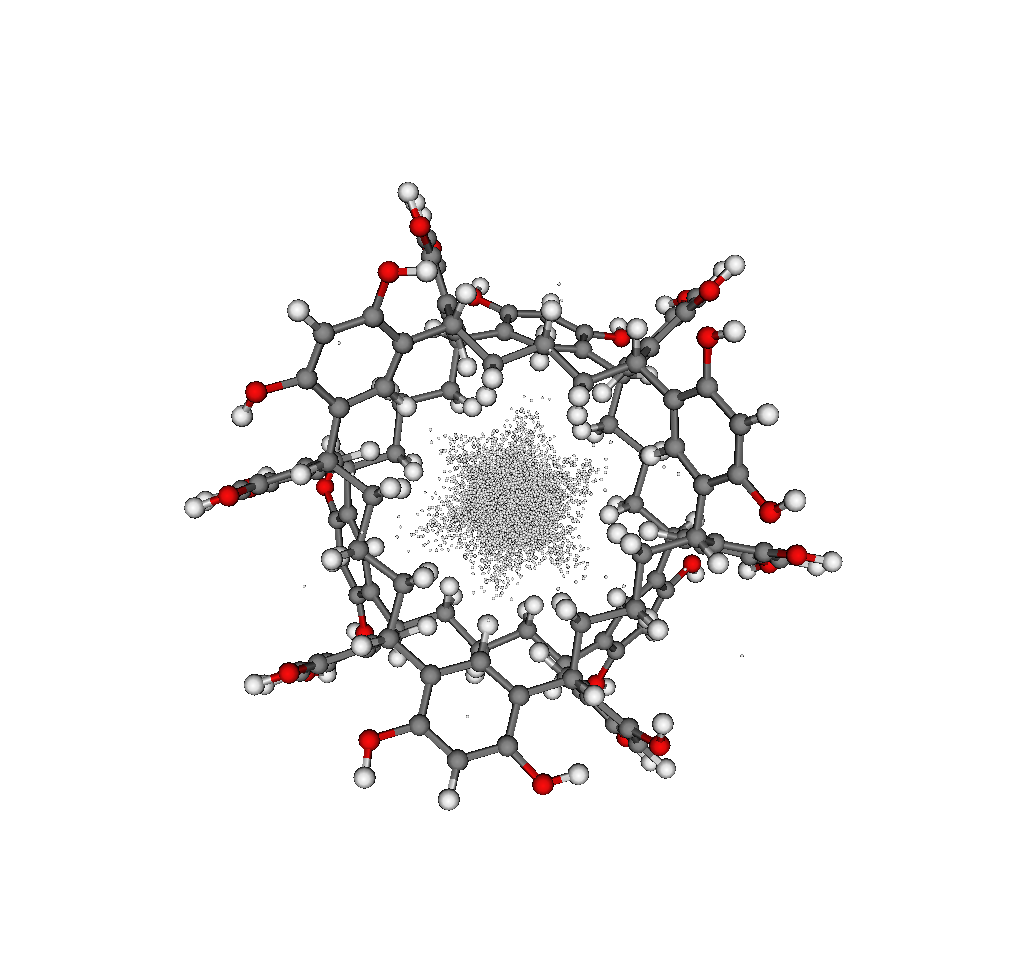
\includegraphics[width=0.45\columnwidth]{NC2_porosity_point_cloud.png}
	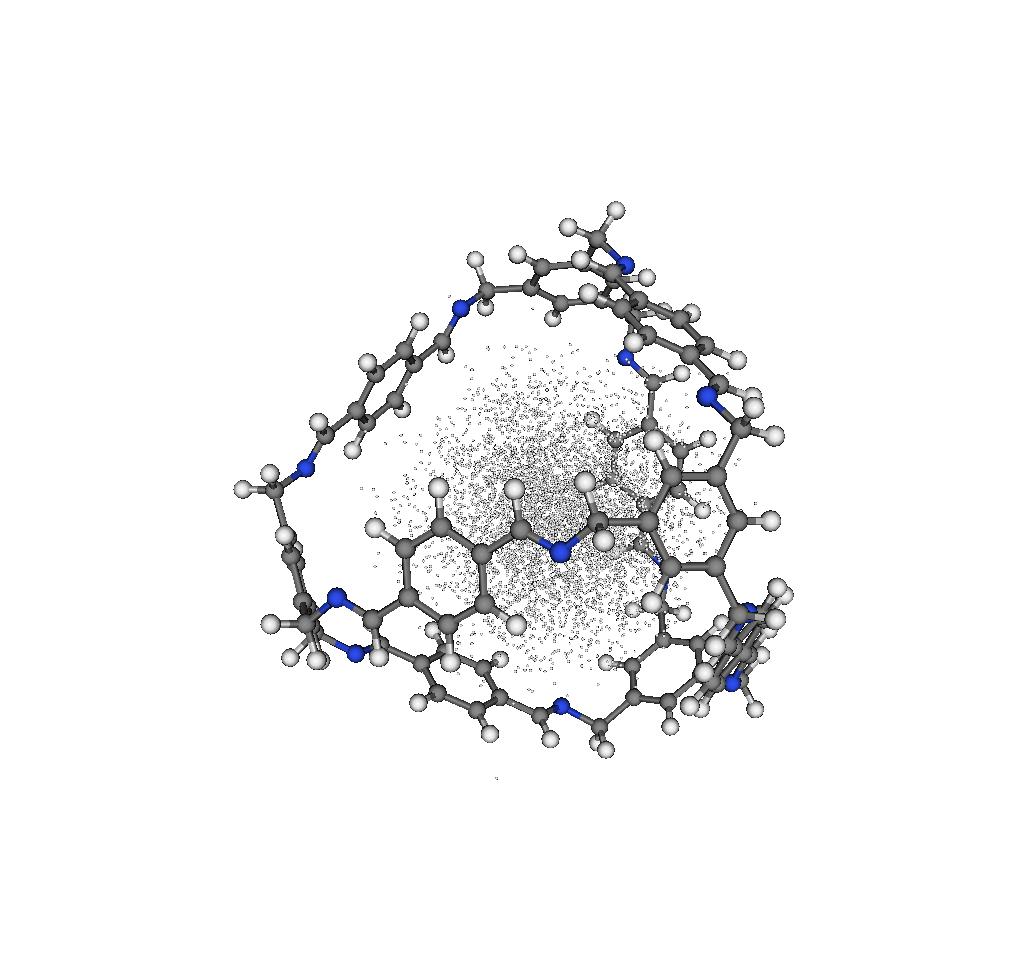
\includegraphics[width=0.45\columnwidth]{A11_porosity_point_cloud.png}
	\caption{The porosity point clouds (5000 points each) generated to describe the cavity of \textbf{NC2} (left) and \textbf{A11} (right) are shown along with the cage structures.
	} \label{fig:porosity_pt_cloud}
\end{figure}

\subsection{First attempt: alignment on the basis of rotational dynamics}
\label{sec:alignment_details}
We compute the $3\times 3$ symmetric moment of inertia matrix $\mathbf{M}$ of the porosity point cloud of each cage, defined relative to the center of mass of the cage, and find its eigendecomposition $\mathbf{M}=\mathbf{W}\mathbf{\Lambda}\mathbf{W^T}$, with the eigenvalues arranged in a non-increasing order down the diagonal matrix $\mathbf{\Lambda}$ and the orthonormal eigenvectors in the columns of $\mathbf{W}$. The eigenvectors of the matrix $\mathbf{M}$ are the principal axes of inertia, and the associated eigenvalues are the moments of inertia with respect to those axes, the principal moments of inertia. Then, we transform the coordinates of the centered cage by left-multiplying by the rotation matrix $\mathbf{W^T}$. The porosity point cloud of the rotated cage then possesses a diagonal moment of inertia matrix with the moments of inertia arranged in a non-increasing order down the diagonal. Next, we will show that for some cages, the rotational dynamics of the porosity point cloud do not provide a reasonable means to consistently align them. For only 18 of the cages did we use the principal axes of inertia to align them.


\subsection{Degenerate principal axes of inertia}
\label{sec:degenerate}
The porosity point clouds of cage molecules that exhibit a degree of symmetry can possess degenerate moments and principal axes of inertia. As a pedagogical example, consider sulfur trioxide (SO$_3$), a trigonal planar molecule, shown in Fig.~\ref{fig:SO3}. Its moment of inertia matrix $\mathbf{M}$ about the center of the molecule (the S atom), with Cartesian directions defined in Fig.~\ref{fig:SO3} and the sulfur atom at the origin, is:
\begin{equation}
\mathbf{M} = m_{\text{O}} \ell_{S-O}^2
  \begin{bmatrix}
    3/2 & 0 & 0 \\
    0 & 3/2 & 0 \\
    0 & 0 & 3
  \end{bmatrix}, \label{eq:I_SO3}
\end{equation} where $m_{\text{O}}$ is the mass of an oxygen atom and $\ell_{S-O}$ is the sulfur-oxygen bond length. The eigenvalues of the moment of inertia matrix $\mathbf{M}$ and thus principal moments of inertia are 3/2, 3/2, and 3 times $m_{\text{O}} \ell_{S-O}^2$. The eigenvector (unique if unit norm enforced) associated with the largest eigenvalue, $3 m_{\text{O}} \ell_{S-O}^2$, is $[0, 0, 1]$, indicating that the principal axis of inertia with the largest moment of inertia is pointing out of the page with respect to Fig.~\ref{fig:SO3}. The remaining two principal axes of rotation must be orthogonal to $[0, 0, 1]$ and thus lay in the $x$-$y$ plane. The moments of inertia about the remaining two principal axes of rotation, however, are equal, as the remaining eigenvalues 3/2, 3/2 times $m_{\text{O}} \ell_{S-O}^2$ are degenerate. In fact, \emph{any} vector laying in the $x$-$y$ plane is an eigenvector of the matrix $\mathbf{M}$ in eqn.~\ref{eq:I_SO3} associated with eigenvalue $3m_{\text{O}} \ell_{S-O}^2/2$. This mathematically indicates that the two remaining principal axes of rotation for SO$_3$ are not unique; any two sets of orthogonal vectors lying in the $x$-$y$ plane will serve as principal axes of rotation of the SO$_3$.

\begin{figure}
\centering
	\subfloat[][]{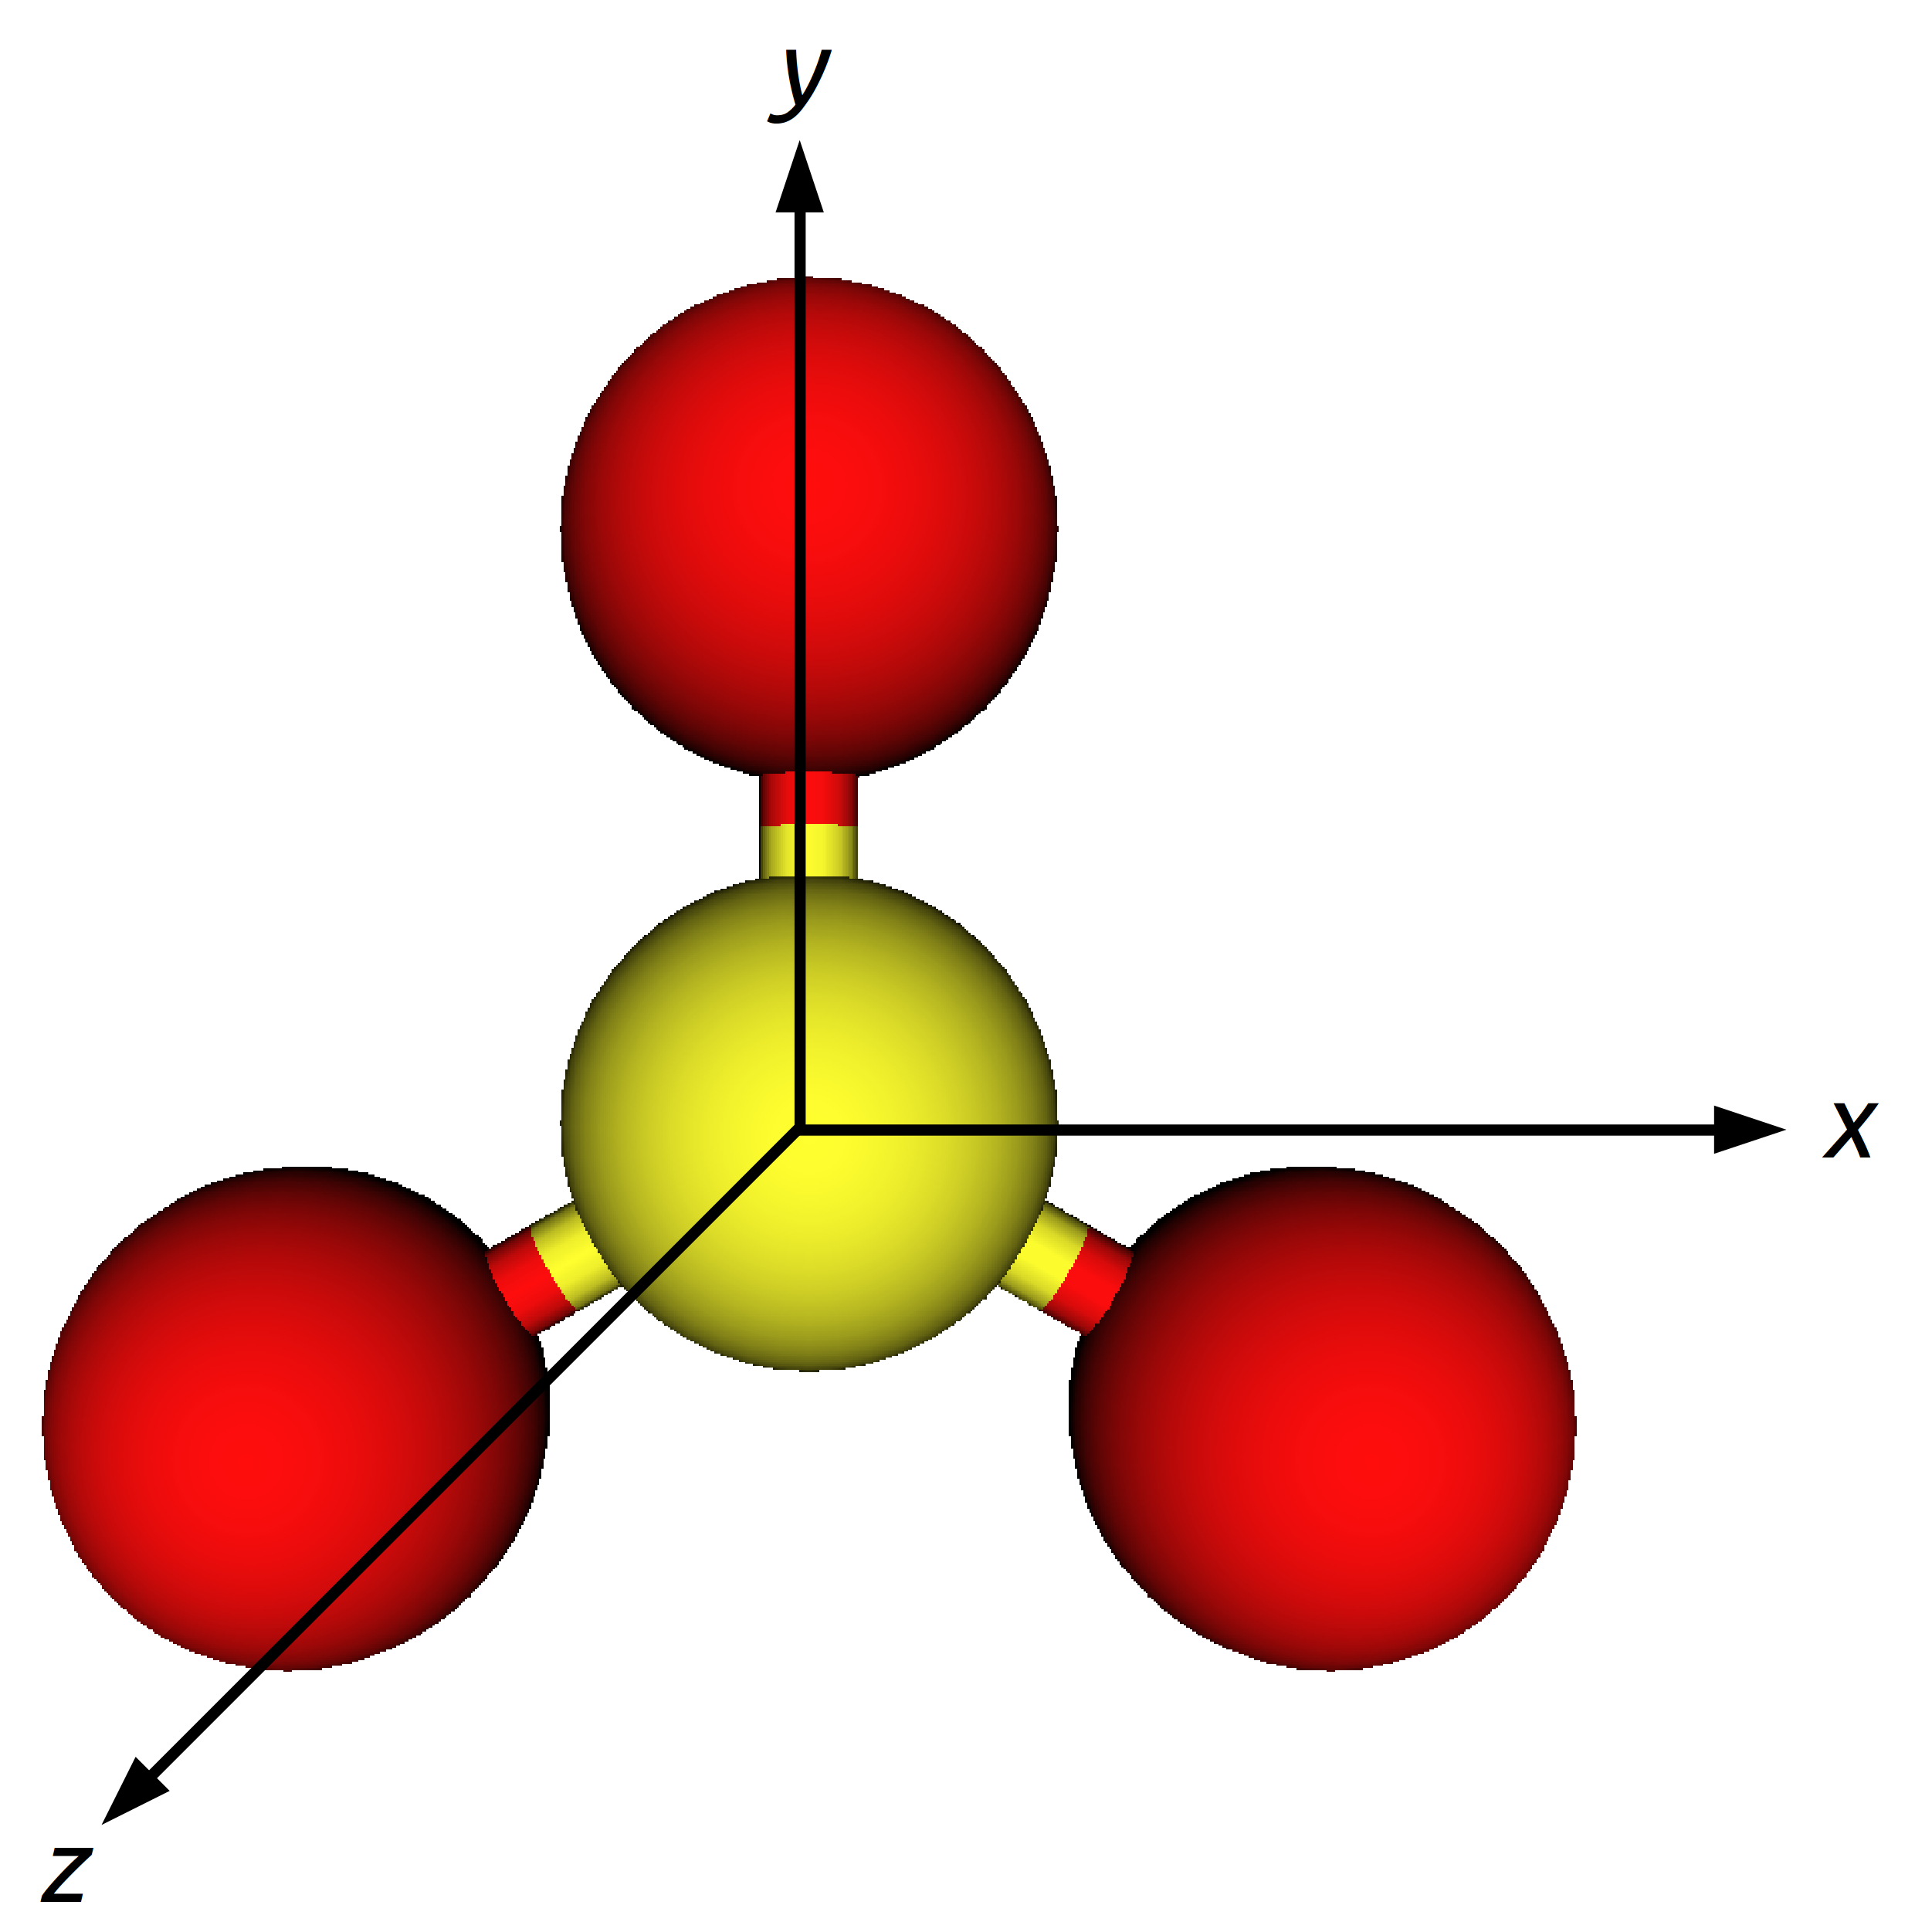
\includegraphics[width=0.3\columnwidth]{../principal_axes_rotation_failure/SO3_axes_marked.png} \label{fig:SO3}}
	\subfloat[][]{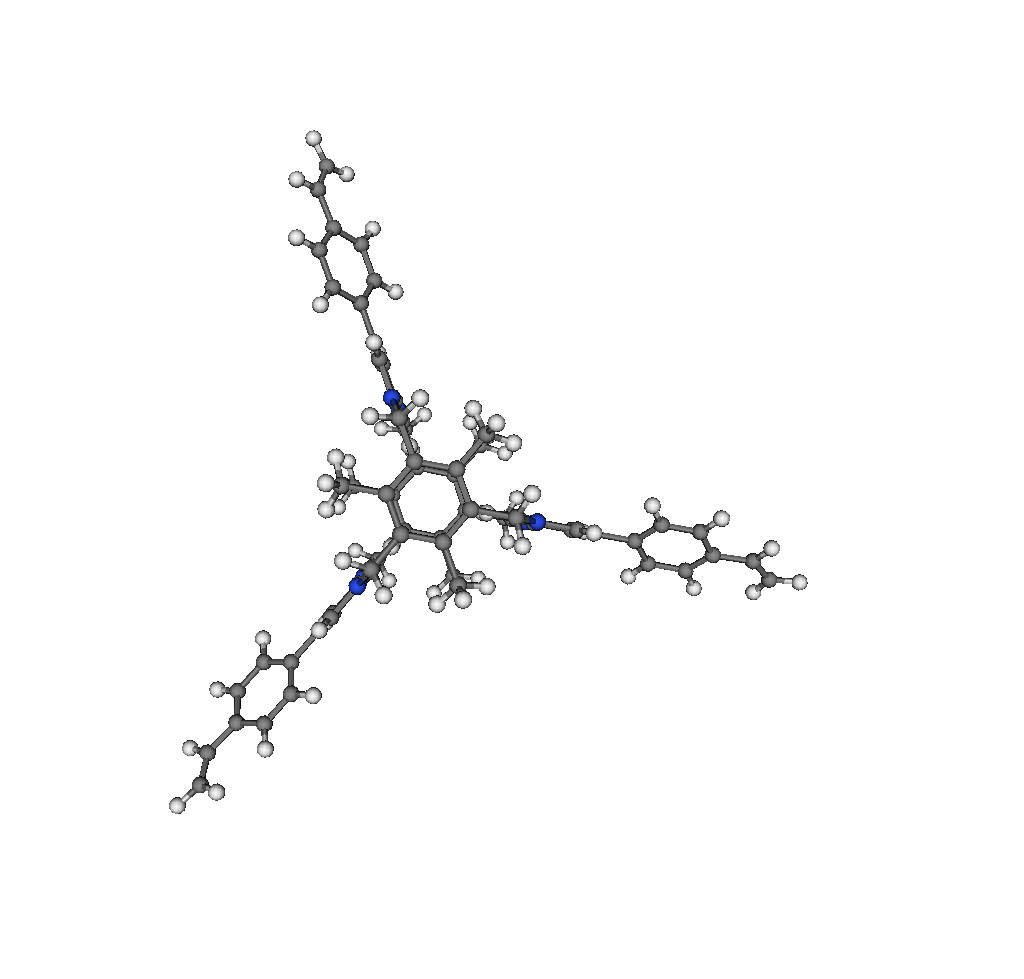
\includegraphics[width=0.5\columnwidth]{B6_propeller.png} \label{fig:B6_propeller}}
	\caption{When the principal axes of rotation are not uniquely defined. (a) Sulfur trioxide (SO$_3$) is a trigonal planar molecule with degenerate principal axes of rotation in the $x$-$y$ plane. (b) \textbf{B6} is a cage molecule whose rotational dynamics resemble SO$_3$ and thus exhibits nearly degenerate principal axes of rotation in one plane (the plane of the page).
	} \label{fig:irrationallyaligned}
\end{figure}

As a consequence, the principal axes of rotation for a symmetric molecule such as SO$_3$ do not provide a means to uniquely align the molecule. Thus, e.g. to compare SO$_3$ to a molecule exhibiting the same trigonal planar symmetry, such as boron trifluoride BF$_3$, the principal axes of rotation cannot be used to align the two molecules along their bonds (aside from the principal axes of rotation associated with the largest moment of inertia, $[0, 0, 1]$ in Fig.~\ref{fig:SO3}). With regards to its rotational dynamics, SO$_3$ behaves as a uniform disk \cite{peraire2008lecture}.

The cavities of several cage molecules exhibit a high degree of symmetry, so as to behave akin to SO$_3$, where the principal axes of rotation are not unique and thus cannot be used to consistently align them. Interestingly, juxtapose cage \textbf{B6} in Fig.~\ref{fig:B6_propeller} with SO$_3$, which resembles a three-blade propeller \cite{peraire2008lecture} with nearly degenerate principal axes of rotation in one plane. While we focused on the porosity point clouds to align the cages more on the basis of their cavity shapes, as opposed to focusing directly on the atoms of the cage, the idea is the same: the porosity point clouds of many cages harbor rotational dynamics akin to a sphere or disk, where the principal axes of rotation are degenerate and thus sensitive to small differences in the structure/cavity shape. 

For example, the three moments of inertia of the porosity point clouds of \textbf{CC1} and of \textbf{CC3} differ by less than 1\%, indicating that the rotational dynamics of \textbf{CC1} and \textbf{CC3} are akin to a sphere; therefore, using the principal axes of rotation to align \textbf{CC1} and \textbf{CC3} (i) theoretically will not provide a unique manner in which to align them and (ii) will be extremely sensitive to small perturbations in the structure and small differences in the randomly chosen points comprising the porosity point cloud. Note that \textbf{CC3} and \textbf{CC1} differ only in the vertices external to the cavity, but, as Fig.~\ref{fig:misaligned} shows, \textbf{CC1} and \textbf{CC3} are aligned irrationally on the basis of their computed principal axes of rotation due to the [near-]degeneracy of their axes of rotation. Another example that is highly related to the SO$_3$ example in Fig.~\ref{fig:SO3} are \textbf{B6} and \textbf{B8}, also shown in Fig.~\ref{fig:misaligned}. Here, small differences in the three propeller-blade-like moieties that protrude from \textbf{B6} and \textbf{B8} as well as small differences in the random positions in the porosity point cloud result in significantly inconsistent alignments for comparing \textbf{B6} and \textbf{B8}. \textbf{B6} and \textbf{B8} much resemble the SO$_3$ example in Fig.~\ref{fig:SO3}, as two principal axes of rotation are nearly degenerate and thus the principal axes in that plane (the plane of the page in Fig.~\ref{fig:allcagesdetailed}) are very sensitive to small perturbations in the structure.

\begin{figure}
\centering
	\subfloat[][CC3]{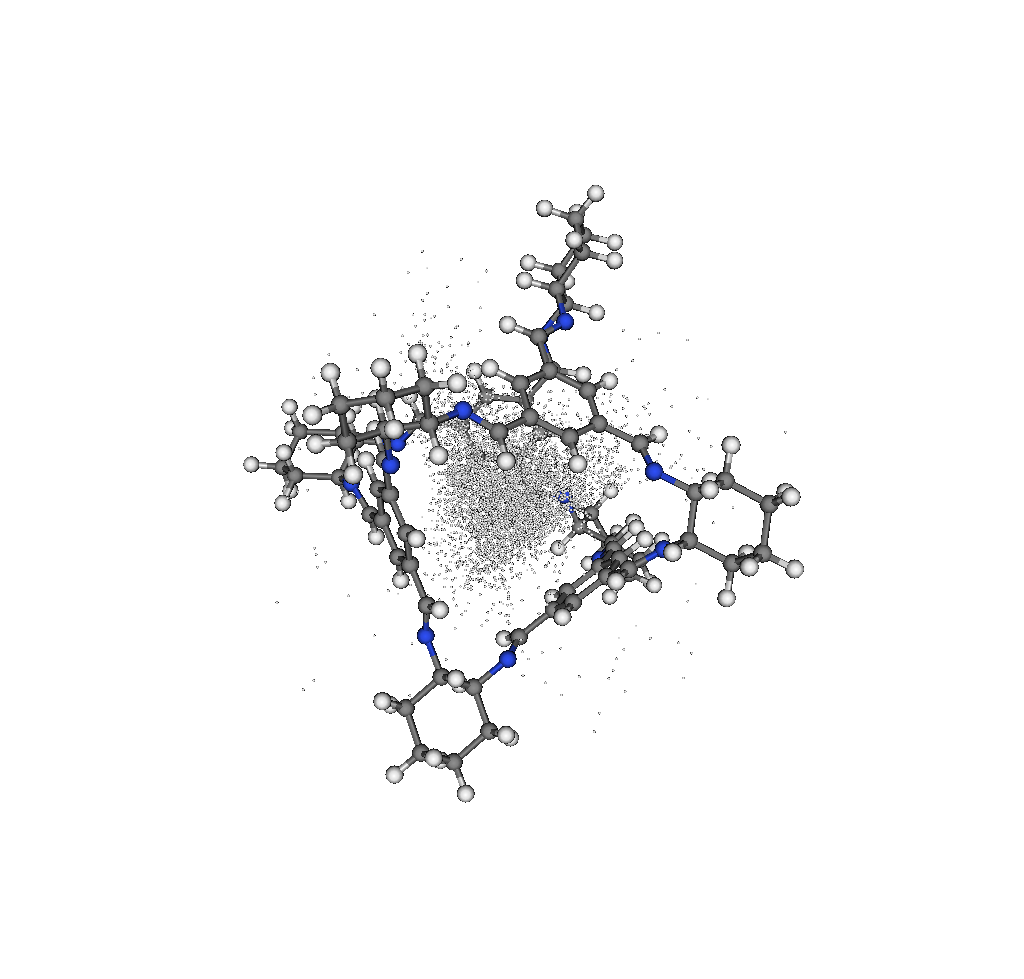
\includegraphics[width=0.45\columnwidth]{CC3_porosity_point_cloud.png}}
	\subfloat[][CC1]{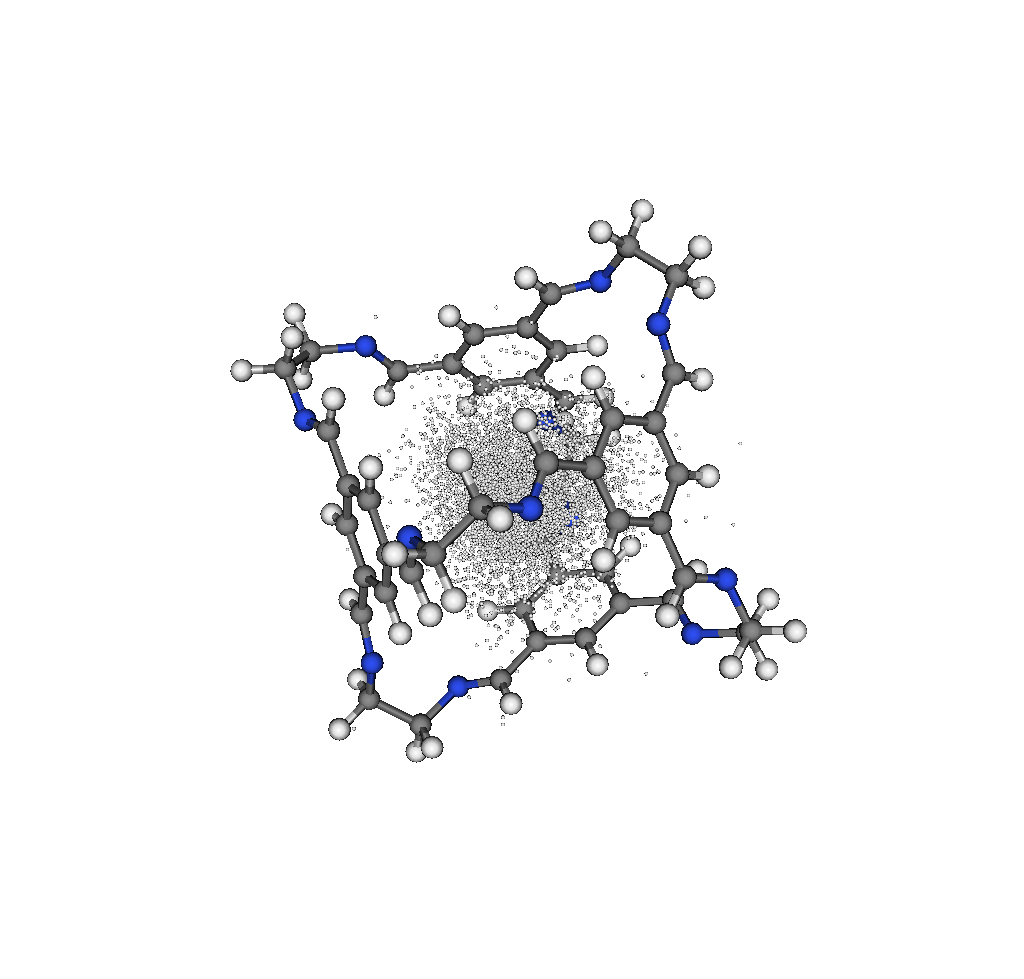
\includegraphics[width=0.45\columnwidth]{CC1_porosity_point_cloud.png}} \qquad
		\subfloat[][B6]{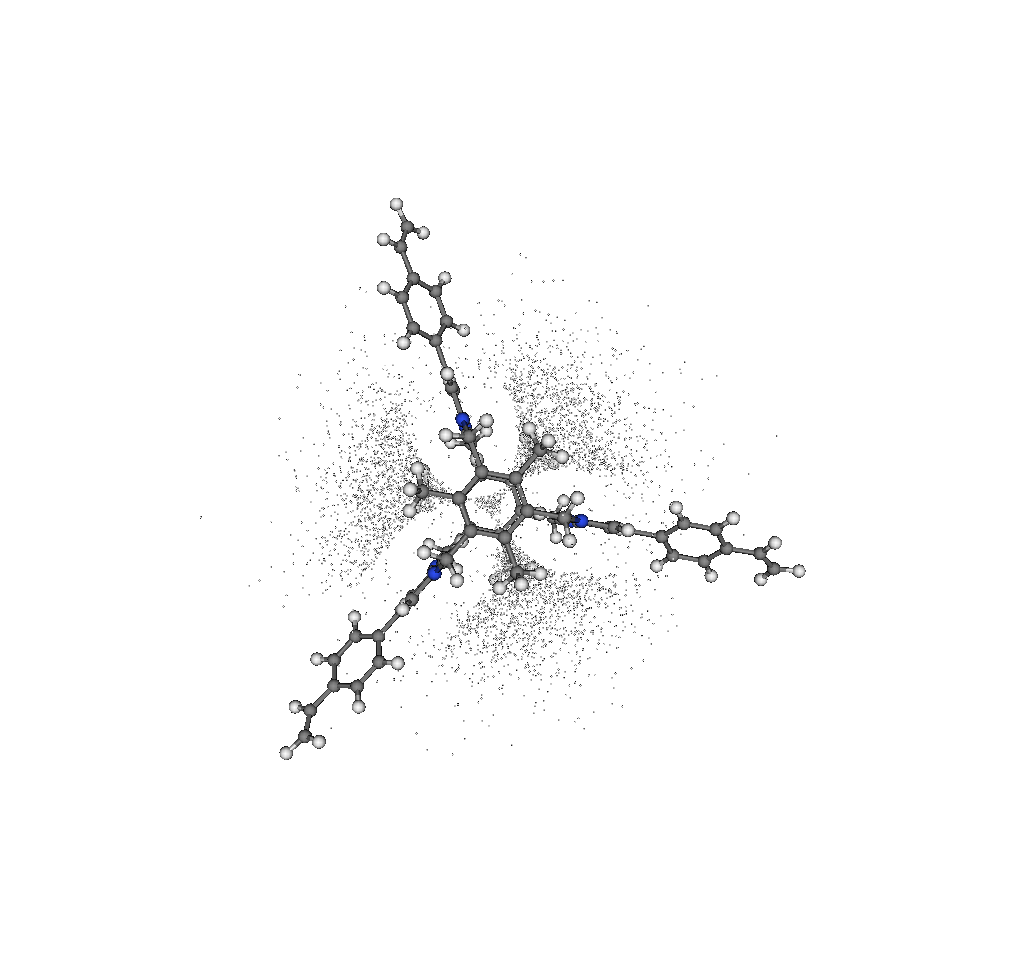
\includegraphics[width=0.45\columnwidth]{B6_porosity_point_cloud.png}}
	\subfloat[][B8]{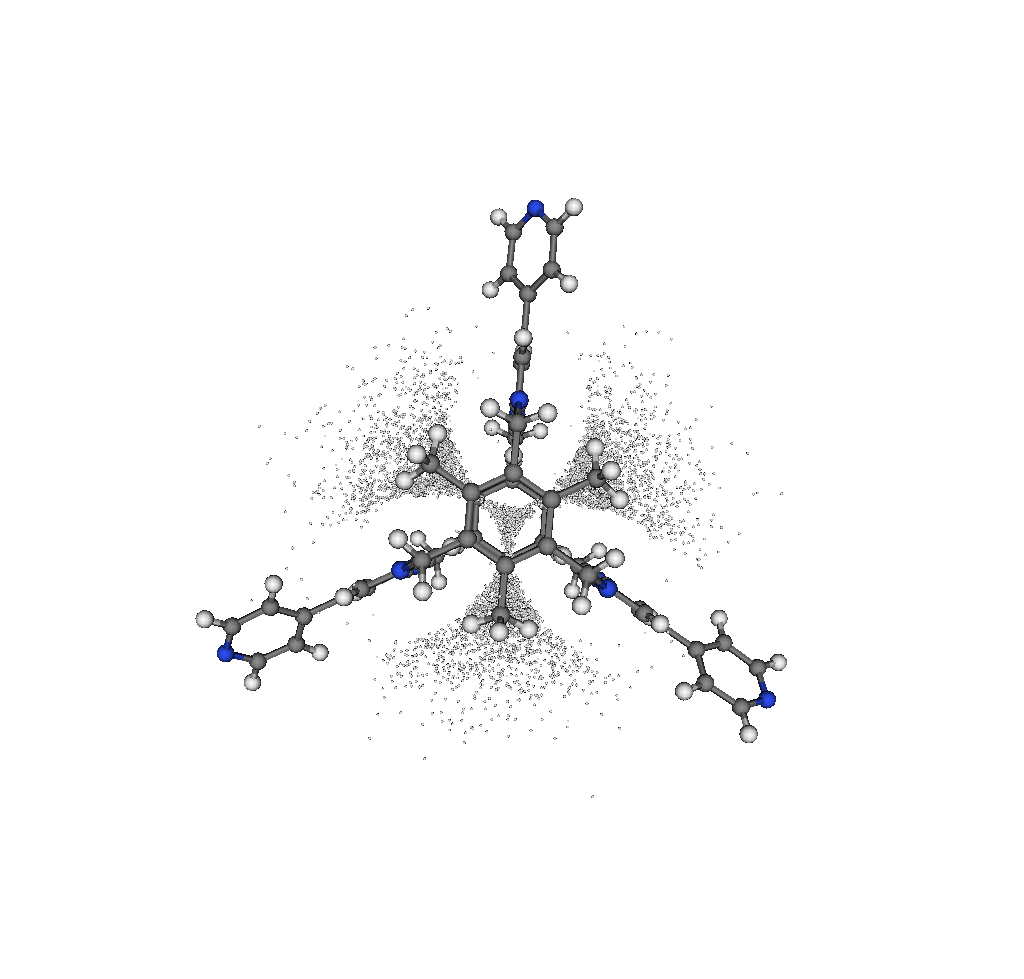
\includegraphics[width=0.45\columnwidth]{B8_porosity_point_cloud.png}}
	\caption{Cases where the computed principal axes of rotation of the porosity point clouds do not provide reasonable alignments of cages. Shown are the porosity point clouds and structures of four cages. (a, b) The rotational dynamics of \textbf{CC1} and \textbf{CC3} are akin to a sphere; the three moments of inertia of the porosity point clouds for each \textbf{CC1} and \textbf{CC3} are computed to differ less than 1\% from one another. Shown are the two cages aligned with the computed principal axes of rotation of their porosity point clouds. Despite the structures differing only in the their vertices at the periphery of the cage, the two cages are aligned inconsistently/irrationally. (c, d) Shown are cages \textbf{B6} and \textbf{B8} aligned with the principal axes of rotation of their porosity point clouds. \textbf{B6} and \textbf{B8} have two nearly degenerate axes of rotation in the plane of the page. As a result, despite only subtle differences in the three propeller-blade-like moieties that protrude from their cores and small differences in the random positions in the porosity point clouds, these two cages are aligned irrationally.
	} \label{fig:misaligned}
\end{figure}

Therefore, the principle axes of rotation are in many cases insufficient to determine an alignment of a porous cage molecule that is unique and robust to small differences. The set of cages whose porosity point clouds display successive principal moments of inertia that differ by greater than one percent are in Table~\ref{tbl:aligned_via_rotational_dynamics}. Only for these cages did we give the principal axes of rotation the authority to align them. For the remaining cages, whose rotational dynamics resemble those of a sphere or disk with practically arbitrary principal axes of rotation, we resorted to employing the Coherent Point Drift algorithm to pairwise align cages as described in the ``Alignment'' section in the main text. For the remaining cages not present in Table~\ref{tbl:aligned_via_rotational_dynamics}, Table~\ref{tbl:aligned_via_coherent_point_drift} shows the result of which cages where aligned to which cages (in order of top to bottom) on the basis of their porosity point clouds, using the Coherent Point Drift algorithm. The Julia code for our Coherent Point Drift algorithm can be found at \url{https://github.com/SimonEnsemble/CoherentPointDrift.jl}.


\begin{table}[h!]
  \caption{List of cages aligned on the basis of the authoritative rotational dynamics of their porosity point clouds.}
  \label{tbl:aligned_via_rotational_dynamics}
  \centering
  \begin{tabular}{c}
    \toprule
B13 \\
C13 \\
C20 \\
CB5 \\
CB6 \\
CB7 \\
CD1 \\
CP1 \\
CP3 \\
CP4 \\
CP5 \\
IC2 \\
MC3 \\
NC1 \\
NC2 \\
RCC3a \\
WC2 \\
WC3 \\
    \bottomrule
  \end{tabular}
\end{table}

\begin{longtable}{cc}
\hline
 \textbf{Cage}  & \textbf{aligned to...}  \\
 \hline
 CC2 & CP1\\
 WC4 & CP3\\
 HC1 & CP4\\
 CD2 & CP3\\
 CC9 & CP1\\
 CC4 & CP3\\
 CC3 & CP3\\
 RCC3b & CP3\\
 RCC1d & CB5\\
 CC10 & CP1\\
 CD3 & CB7\\
 A11 & CD1\\
 B11 & CD1\\
 CC1 & CP4\\
 RCC1c & CB5\\
 B23 & CD1\\
 CC5 & CC1\\
 C11 & CB7\\
 C23 & CD1\\
 MC4 & CC1\\
 MC7 & CD1\\
 WC1 & CP4\\
 B15 & CC2\\
 MC5 & CD2\\
 C15 & CC2\\
 B24 & CD3\\
 MC2 & HC1\\
 C24 & IC2\\
 DC1 & CP1\\
 MC1 & HC1\\
 B18 & RCC1d\\
 B25 & NC2\\
 C18 & CC4\\
 C25 & CD3\\
 GC1 & RCC1d\\
 B26 & RCC1d\\
 IC1 & CC3\\
 C26 & RCC1d\\
 RCC1b & CB5\\
 MC6 & B24\\
 RCC1a & CP4\\
 B1 & CP4\\
 B2 & B1\\
 B9 & B2\\
 C8 & B2\\
 C2 & B1\\
 C9 & C2\\
 B8 & C2\\
 C1 & B1\\
 C6 & B2\\
 B6 & C8\\
 C5 & C2\\
 C4 & B8\\
 B4 & B8\\
 B5 & B8\\
 C21 & B6\\
    \hline
          \caption{List of cages whose porosity point clouds harbored rotational dynamics that approximate those of a sphere or disk and thus are not authoratative for aligning them. This table shows which cage these cages were aligned to, in order from top to bottom, on the basis of their porosity point clouds and using the Coherent Point Drift algorithm.}
  \label{tbl:aligned_via_coherent_point_drift}
\end{longtable}

\clearpage
\newpage

\section{The data matrix $\mathbf{A}$}

\begin{figure}
\centering
	\includegraphics[width=\columnwidth]{../data_matrix_viz.png}
	\caption{An attempt at visualizing the structure of the $c \times g^3$ data matrix $\mathbf{A}$. The color depicts the magnitude of the entry of the matrix. This is an ``attempt'' because $g^3>>c$, so the data matrix $\mathbf{A}$ is wide and difficult to visualize without a much longer page. We remark that 48334/125000 of the columns (representing pixels in the 3D porosity images of the cages) are non-zeros.
	} \label{fig:data_matrix}
\end{figure}

\newpage
\clearpage

\section{The singular values of $\mathbf{A}$}

\begin{figure}
\centering
	\includegraphics[width=0.65\columnwidth]{../distn_of_svs.png}
	\caption{The distribution of the set of singular values $\sigma_1,\sigma_2, ..., \sigma_{74}$ of $\mathbf{A}$.
	} \label{fig:distn_of_svs}
\end{figure}

\newpage
\clearpage

\section{Relative error from approximating $\mathbf{A}$ as $\mathbf{A}_\nu$}

\begin{figure}
\centering
	\includegraphics[width=0.65\columnwidth]{../relative_err_with_svs.png}
	\caption{The relative error in approximating the data matrix $\mathbf{A}$ with a lower-rank-$\nu$ approximant $\mathbf{A}_\nu$ given in eqn.~\ref{eq:Anu}. The formula for the relative error as a function of $\nu$, related to the singular values of $\mathbf{A}$, is given in eqn.~\ref{eq:relative_error}.
	} \label{fig:relative_err_with_svs}
\end{figure}

\newpage
\clearpage

\section{Highlighting remaining clusters in latent cage space}

\begin{figure}[h!]
\centering
	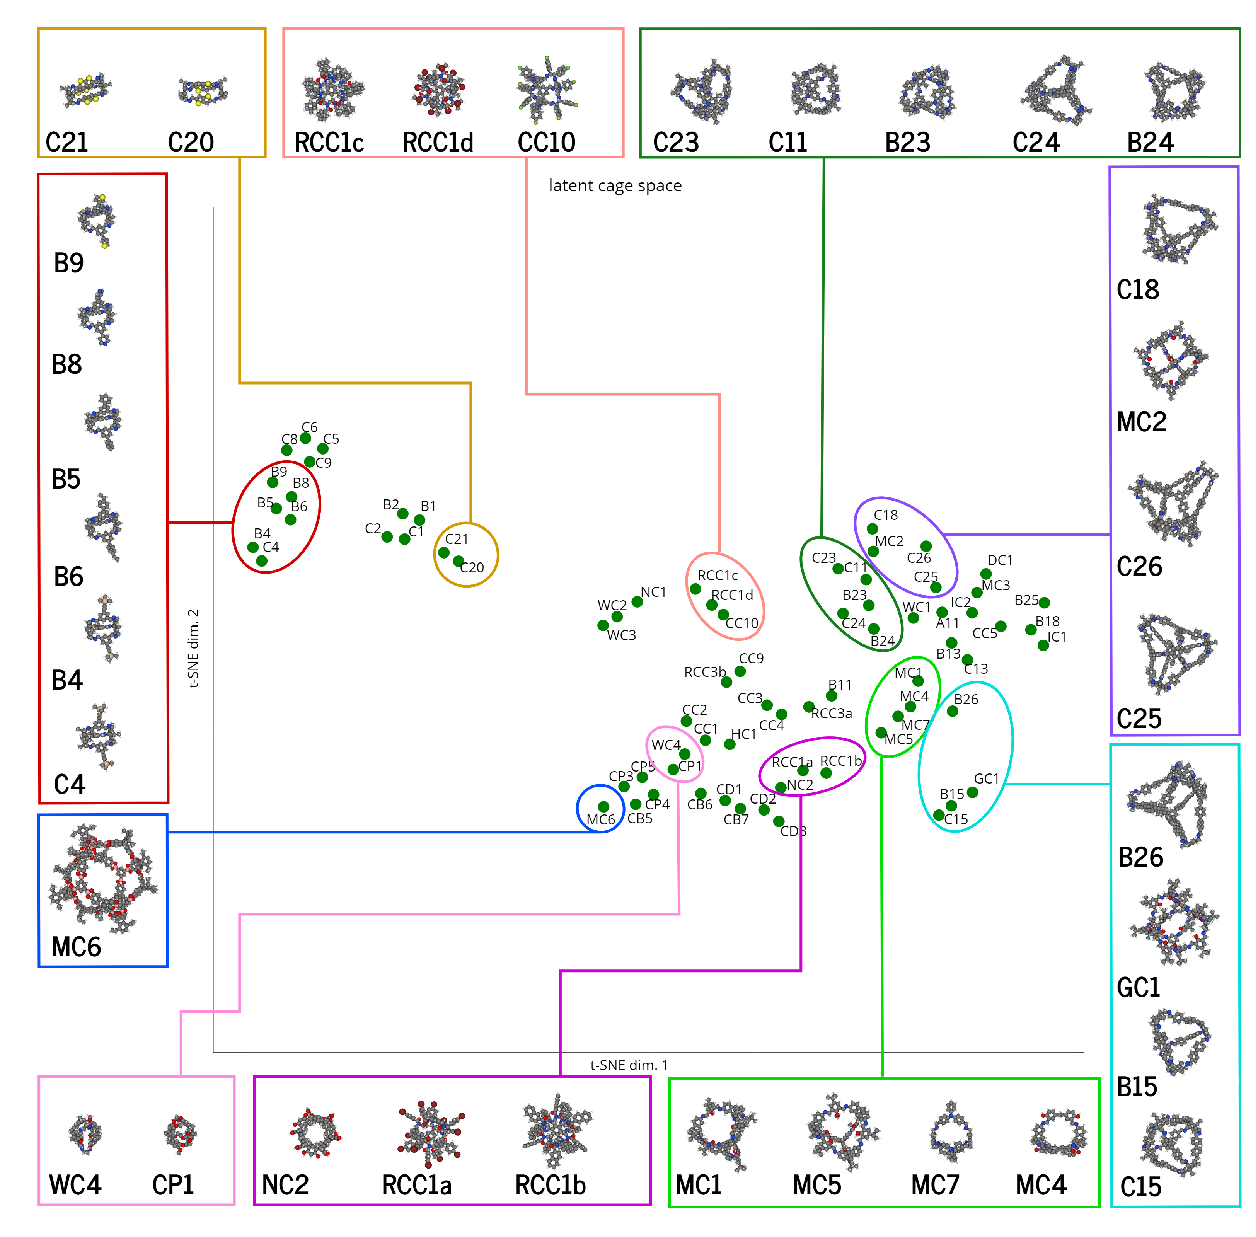
\includegraphics[width=0.9\columnwidth]{../latent_cage_space_2D_marked_SI.pdf}
	\caption{The latent space of cages $\mathbf{U}_\nu \mathbf{\Sigma}_\nu$ embedded into 2D by t-SNE \cite{maaten2008visualizing,wattenberg2016how}. Salient clusters are highlighted. See Fig.~\ref{fig:latent_space} for the remaining clusters.
	} \label{fig:latent_space2}
\end{figure}


\newpage
\clearpage


\section{Henry coefficient calculations} \label{sec:henrydetails} We describe more details here of the Henry coefficient calculations used to obtain the data in Fig.~\ref{fig:latent_space_S_Xe_Kr}. We model the energetics of the interaction of a gas atom (Xe, Kr, He) with the atoms of the cage as pairwise additive and with 12-6 Lennard-Jones potentials. The $\epsilon_i$ and $\sigma_i$ parameters of the Lennard-Jones potentials for atom $i$- atom $i$ interactions are taken from the Universal Force Field \cite{rappe1992uff} (cutoff radius 14~$\angstrom$). Geometric mixing rules are applied for cross-interactions. 

We placed an isolated cage molecule in an empty simulation box and took it as rigid. If $\mathbf{x} \in \mathbb{R}^3$ is the position of a gas atom in the simulation box, the molecular model described above gives us the potential energy of the gas molecule, $U(\mathbf{x})$.

Consider the isolated porous cage molecule immersed in a bath of gas; the simulation box is drawn around the porous cage molecule. Henry's law models the density of gas in the simulation box at thermodynamic equilibrium, $\rho $, as $\rho=K P$, with $K$ the Henry coefficient and $P$ the pressure of the gas. Henry's law is valid only at low surface coverage.

The Henry coefficient of a gas in the simulation box including the isolated cage molecule is given as:
\begin{equation}
K = \beta \frac{1}{|\Omega|} \int_\Omega e^{-\beta U(\mathbf{x})} d\mathbf{x},
\label{eq:K}
\end{equation} where $\beta= (k_B T)^{-1}$ is the thermodynamic beta ($T$ temperature, $k_B$ Boltzmann constant) and the integral is over the simulation box $\Omega$ (which has volume $|\Omega|$). Note that if $U(\mathbf{x})=0$, Henry's law recovers the ideal gas law $\rho = \beta P$, where $|\Omega|$ is the volume of the simulation box.

We computed the average in eqn.~\ref{eq:K} via Monte Carlo integration, i.e. Widom particle insertions \cite{frenkel2001understanding}, using 1000 Monte Carlo insertions per volume ($\angstrom^3$) of the simulation box. We used \texttt{PorousMaterials.jl} v0.1.1 \cite{PorousMaterialsJL} to compute the Henry coefficient.

\subsection{Comparing to experimental data}
\label{sec:kh_isolated}
By considering only an isolated cage molecule in a simulation box, as opposed to many cage molecules packed together to form a solid, we account for only the influence of the intrinsic porosity to the cage molecule on the adsorption. This is an approximation, as we are neglecting the influence of the extrinsic porosity that arises from how the cage molecules pack together to form a bulk solid. When the cage molecules pack together, the adsorption sites on the exterior of the molecule or at the cage windows can be modified depending on how the cage molecules pack together. However, when the interior of the cage molecule is the dominant adsorption site in the bulk solid, this approach may be a viable method to predict the Henry coefficient of a bulk porous cage solid.

To evaluate our crude method of considering an isolated cage molecule, Fig.~\ref{fig:expt_sim_compare} compares experimentally measured xenon and krypton adsorption isotherms in noria \cite{patil2016noria} (\textbf{NC2}) and \textbf{CC3} \cite{chen2014separation} to the resulting Henry's law with the Henry coefficient obtained from our simulations. Fig.~\ref{fig:expt_sim_compare} shows this method yields a very good prediction of experimental Xe and Kr Henry coefficients in noria \cite{patil2016noria} (\textbf{NC2}), but underestimates the Henry coefficients in \textbf{CC3} \cite{chen2014separation}. See Patil et. al \cite{patil2016noria} for more discussion.

\begin{figure}
\centering
	\includegraphics[width=0.4\columnwidth]{../noria_expt_sim_comparison.png}
	\includegraphics[width=0.4\columnwidth]{../CC3_expt_sim_comparison.png}
	\caption{Comparison of experimental xenon and krypton adsorption isotherms at 298 K in noria \cite{patil2016noria} and \textbf{CC3} \cite{chen2014separation} to the simulated adsorption. Points show experimental data and the lines show Henry's law with the Henry coefficient taken from our simulations. The simulated Henry coefficient of He was subtracted to account for the empty space in the simulation box.
	} \label{fig:expt_sim_compare}
\end{figure}

\newpage
\clearpage

\section{Relationship of latent representation and cage molecule and cavity diameters}
Fig.~\ref{fig:first_component_captures_pore_diameter} shows that the first component of the learned latent representation of a cage is strongly correlated with its cavity diameter. 
Fig.~\ref{fig:cage_space_colored_by_diams_2D} depicts how the 2D embedding (by t-SNE) of the $\nu=22$ dimensional latent representations is correlated with the molecule diameter and cavity diameter of a porous organic cage molecule.

\begin{figure}
\centering
	\includegraphics[width=0.9\columnwidth]{../first_component_captures_pore_diameter.pdf}
	\caption{The first component of the latent representation of a cage is strongly correlated to its cavity diameter. The cavity diameter was computed by \texttt{pywindow} \cite{miklitz2018pywindow}. In the reconstruction of the 3D porosity image of a given cage, the first component of the latent representation (in the first column of $\mathbf{U}_\nu \mathbf{\Sigma}_\nu$) is the weight on the first eigencage $\mathbf{v}_1$ in the reconstruction of the 3D porosity image via eqn.~\ref{eq:latent_space_view}. That the first eigencage is a good descriptor of pore size is suggested by the radial symmetry of the core of the first eigencage in Fig.~\ref{fig:eigencages} that is added to the approximately radially symmetric average cage $\bar{\mathbf{c}}$ to reconstruct the 3D porosity image via eqn.~\ref{eq:latent_space_view}.
	} \label{fig:first_component_captures_pore_diameter}
\end{figure}


\begin{figure}
\centering
	\includegraphics[width=\columnwidth]{../cage_space_colored_by_diams_2D.pdf}
	\caption{The 2D embedding (by t-SNE) of the learned latent representation of the 3D porosity images contained in the rows of $\mathbf{U}_\nu \mathbf{\Sigma}_\nu$. Here, the diameter of points represents molecule diameter; color represents cavity diameter, both computed by \texttt{pywindow} \cite{miklitz2018pywindow}. Note that neighbors in latent space tend to have similar cavity and molecule diameters.
	} \label{fig:cage_space_colored_by_diams_2D}
\end{figure}

\newpage
\clearpage

\section{Relationship of latent representation and number of windows to enter cavity}

\begin{figure}
\centering
	\includegraphics[width=\columnwidth]{../cage_space_colored_by_nb_windows.pdf}
	\caption{The 2D embedding (by t-SNE) of the learned latent representation of the 3D porosity images contained in the rows of $\mathbf{U}_\nu \mathbf{\Sigma}_\nu$. Here, the color represents the number of windows possessed by the cage molecule. The gas molecules enter the cavity of the cage through the windows. The number of windows is computed by \texttt{pywindow} \cite{miklitz2018pywindow}. Note that cages within clusters in latent space have the same number of windows.
	} \label{fig:cage_space_colored_by_nb_windows}
\end{figure}

\newpage
\clearpage

\section{Assessing effects of flexibility in cages} 
\label{sec:flexibility}

To evaluate how sensitive our methods are to flexibility, four cages (\textbf{CC2}, \textbf{CC3}, \textbf{CC4} and \textbf{CC5}) were allowed to fluctuate at $298$ K in a molecular dynamics (MD) simulation. We considered an isolated, empty cage only. The simulations were performed using GULP v5.0 \cite{gale1997gulp} in the NVT ensemble using the leapfrog Verlet algorithm with the Nose-Hoover thermostat following an initial geometrical optimization of the cage structure. The cage-specific force field (CSFF) was used to model the bond, angle and torsion potentials \cite{holden2012bespoke}; missing parameters were either obtained from the polymer consistent force field (PCFF) \cite{sun1994ab,sun1994force,sun1995ab} as implemented by \texttt{DL$\_$FIELD v4.3} \cite{yong2016dlfield} or a slightly modified version of a PCFF parameter was used. The MD files with every force field parameter can be found on \url{github.com/SimonEnsemble/latent_cage_space/MD_files/*.gin}, where the origin of each potential parameter can be seen in the comments. The CSFF was specifically developed to properly describe porous organic cages. Both Coulombic and Lennard Jones (12-6) potentials were used for interactions between atoms separated by two or more atoms in the bonding graph. Partial charges were assigned to the cage atoms using the parameters provided by the PCFF as given by Holden et al. \cite{holden2012bespoke}. No periodic boundaries were used in these simulations since we considered isolated cage molecules. The equilibration time was $50$ ps while the production time was $1$ ns with a timestep of $0.5$ fs.

We initiated the MD simulation on the aligned cages (as opposed to cage structures taken directly from Miklitz et al. \cite{miklitz2017computational}) rather than going through the process of re-aligning the MD snapshots, due to the excessive computational time required for the Coherent Point Drift algorithm. During the MD simulation, $400$ snapshots of each fluctuating cage were gathered at equally spaced times. To help confirm the validity of the simulations, we calculated the window diameter for each snapshot in \textbf{CC3} using \texttt{pywindow} (Fig.~\ref{fig:window_diameter_hist}). Holden et al.\cite{holden2012bespoke} did a similar analysis of the \textbf{CC3} window diameter during a MD simulation with the before-mentioned CSFF force field, and our distribution of window diameters among the MD snapshots appears to be in good agreement with theirs.

\begin{figure}
\centering
	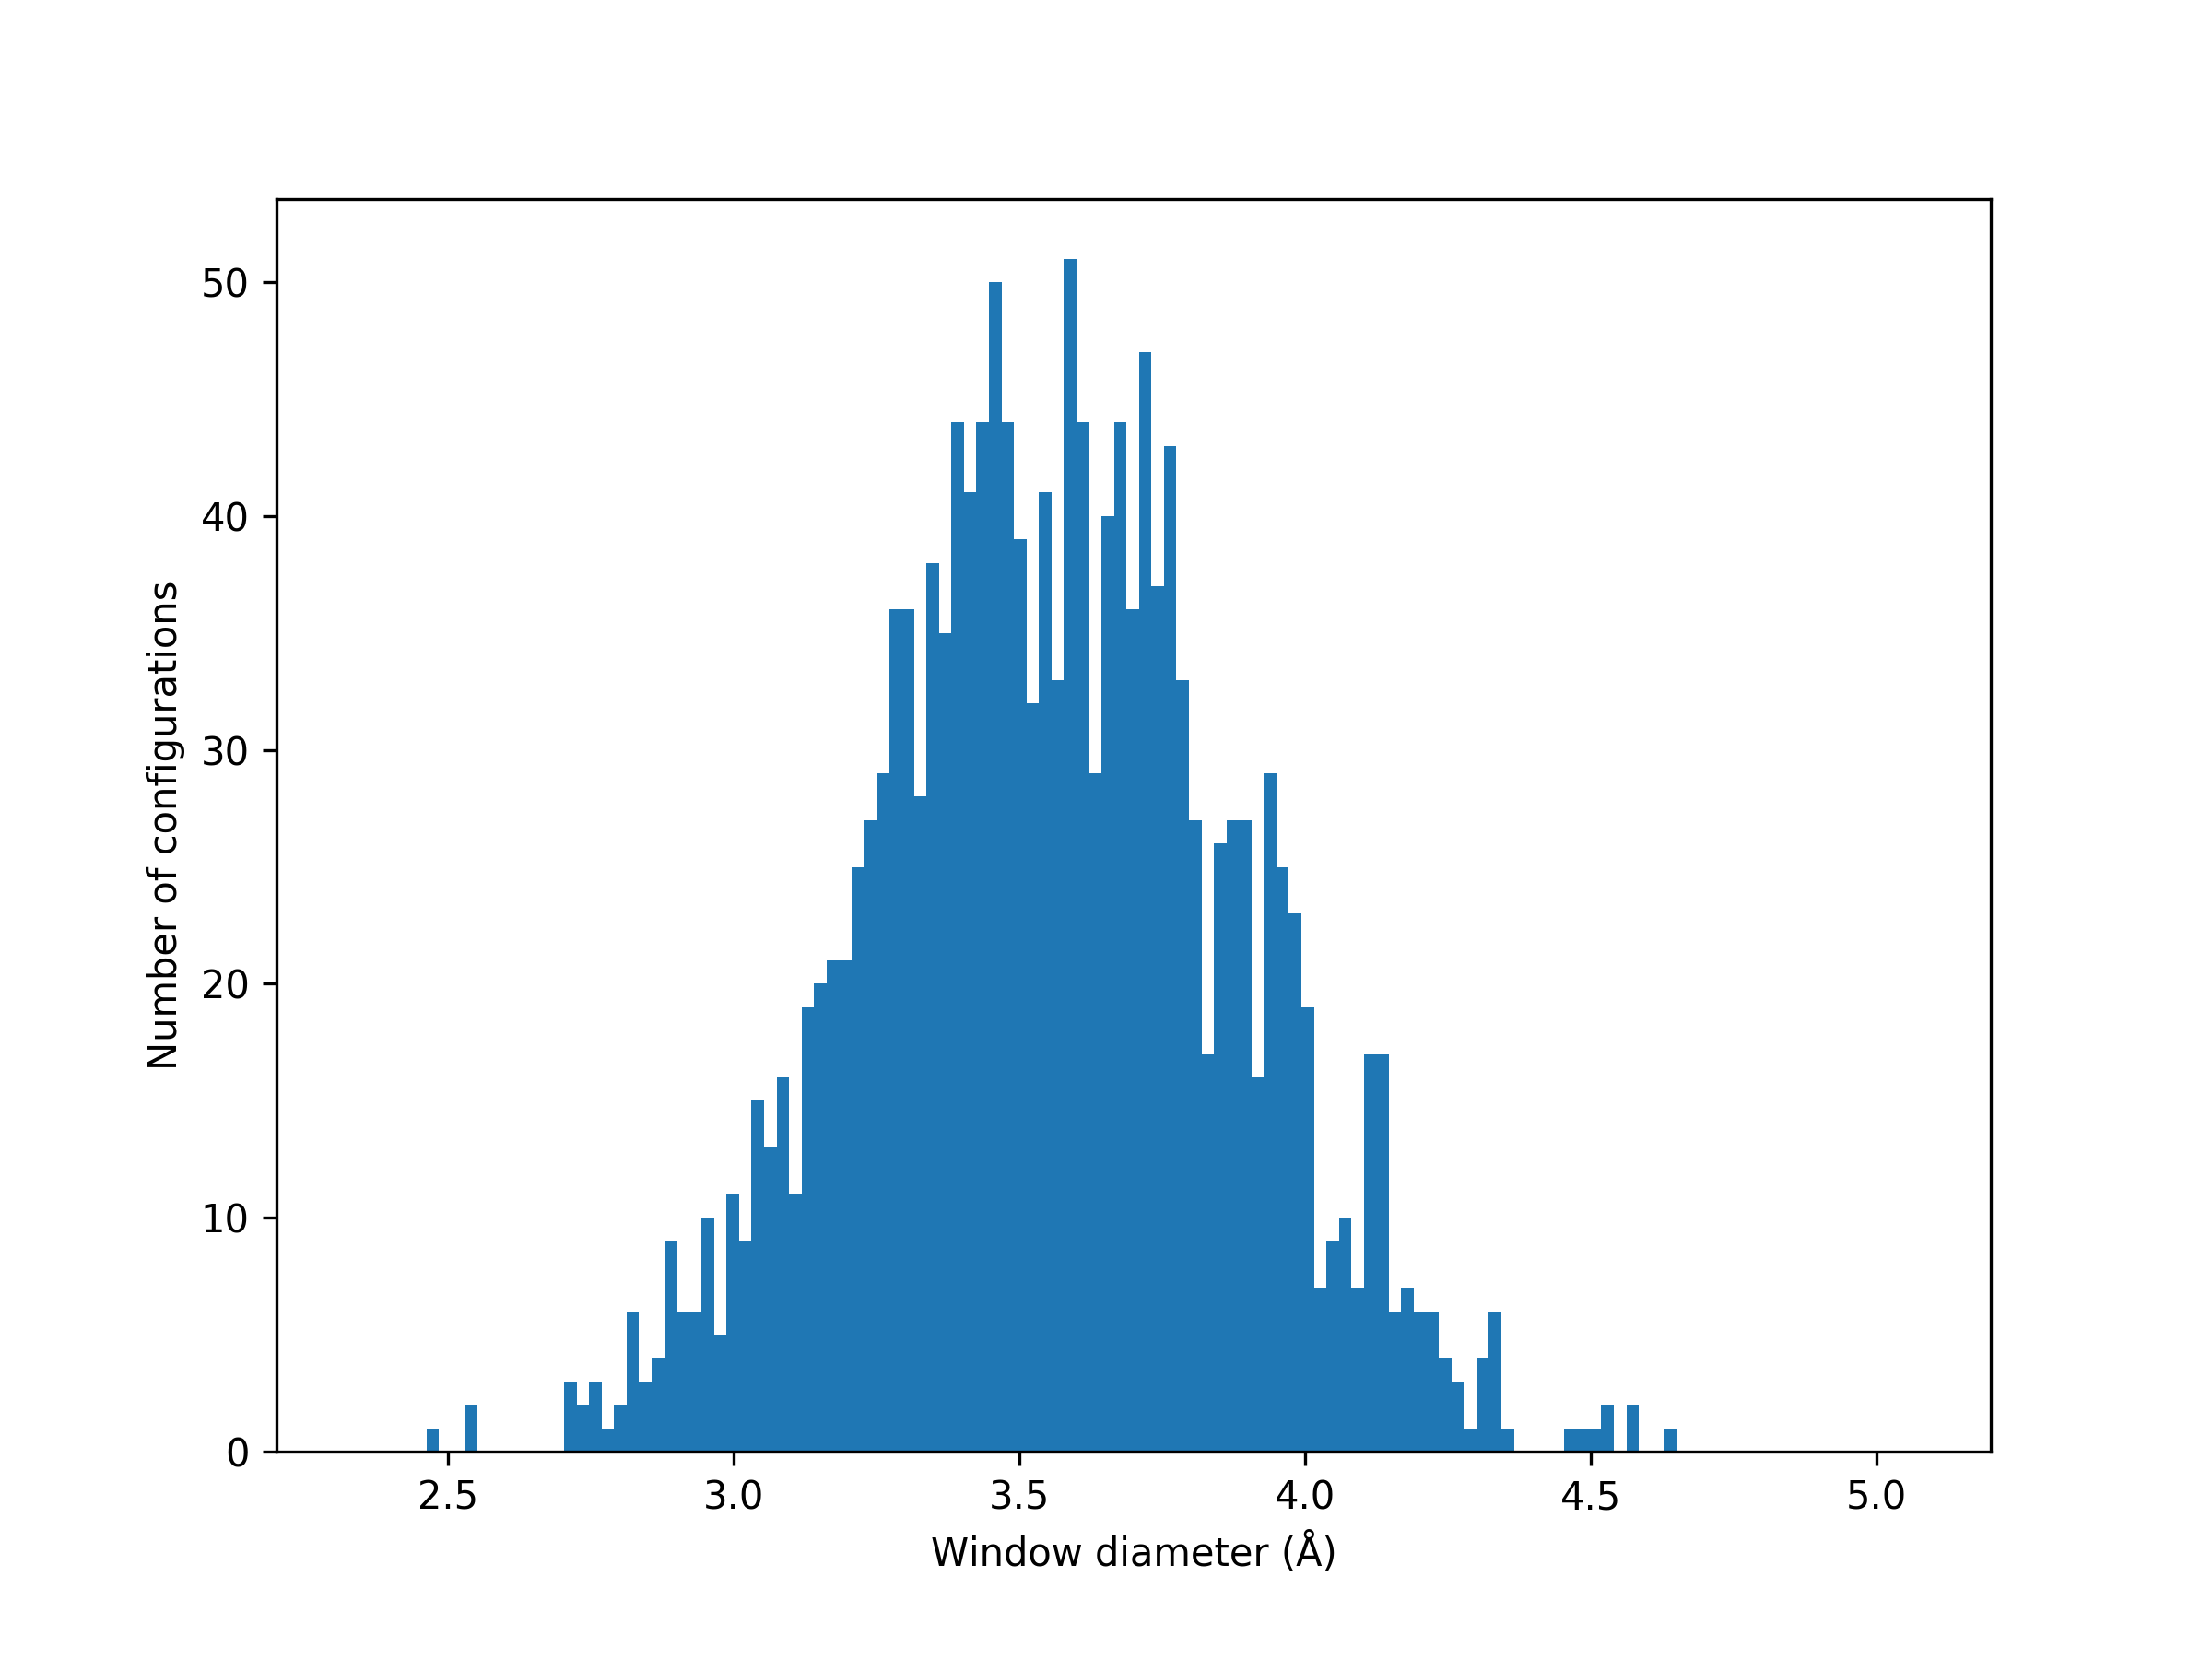
\includegraphics[width=0.65\columnwidth]{../cc3_histogram.png}
	\caption{A histogram of the window diameters, calculated using \texttt{pywindow}, exhibited by each snapshot of \textbf{CC3} from molecular dynamics simulations described above. All four windows of \textbf{CC3} are included.
	} \label{fig:window_diameter_hist}
\end{figure}

We computationally scanned each MD snapshot of the fluctuating cages to generate a 3D porosity image $\mathbf{c}_i$ for each snapshot $i$. We then subtracted off the mean 3D porosity image among the 74 rigid-cage dataset, $\bar{\mathbf{c}}$ to yield $\mathbf{a}_i$.
To visualize where the 3D porosity images of the fluctuating cages are located in latent space, we do not use t-SNE. If t-SNE were used, we would have to retrain it with the inclusion of the fluctuating cages, which would result in overfitting to the large number of fluctuating cages. That is, t-SNE does not learn an explicit mapping function to project new, unseen data points-- the 3D porosity images of the MD snapshots-- onto the embedding in Fig.~\ref{fig:latent_space}. To illustrate how flexible cages move around latent space as their cavity shapes fluctuate, we adopt the simpler choice to project the cages onto our learned latent space $\mathbf{U}_\nu \mathbf{\Sigma}_\nu$ on the basis of the 74 rigid-cage molecules in Fig.~\ref{fig:cages}, but then visualize only the first two latent dimensions. This is equivalent to using a $\nu=2$ dimensional approximant in eqn.~\ref{eq:Anu}, then projecting the MD snapshots of flexible cages onto the $\nu=2$ dimensional latent space. 
The idea here is to best-approximate each 3D porosity image of a snapshot, $\mathbf{a}_i$, as a linear combination of the first two eigencages:
\begin{equation}
\mathbf{a}_i \approx \ell_1 \mathbf{v}_1 + \ell_2 \mathbf{v}_2.
\end{equation} i.e., we aim to project the vector $\mathbf{a}_i$ onto the linear subspace spanned by $\{\mathbf{v}_1, \mathbf{v}_2\}$. Because the eigencages (right singular vectors) $\mathbf{v}_1$ and $\mathbf{v_2}$ are orthonormal, the weights to form the projection are $\boldsymbol \ell := [\ell_1 , \ell_2] = \mathbf{V}_2^T \mathbf{a}_i$ \cite{strang1993introduction}, where $\mathbf{V}_2 = [\mathbf{v}_1 \text{ } \mathbf{v}_2]$ contains the first two eigencages in its columns.

\begin{figure}
\centering
	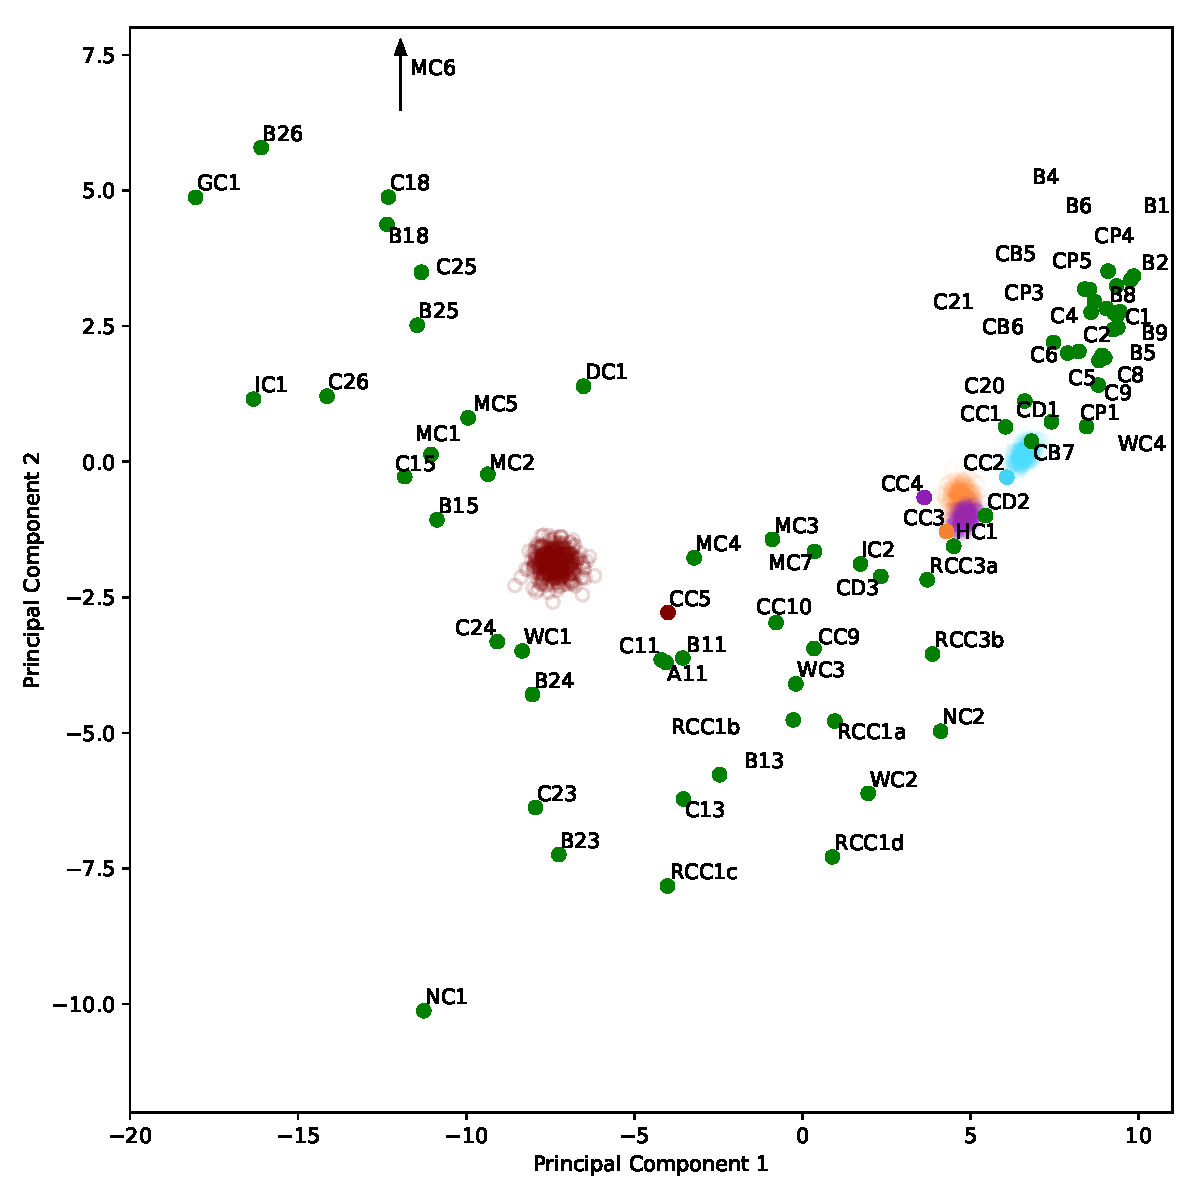
\includegraphics[width=\columnwidth]{../PCA_latent_cage_space_with_flexible_cages_2D.pdf}
	\caption{The black points are the first two dimensions of the latent representations of the (rigid) cages learned by SVD, rows of $\mathbf{U}_2\mathbf{\Sigma}_2$.
The 3D porosity images of snapshots of cages \textbf{CC2}, \textbf{CC3}, \textbf{CC4} and \textbf{CC5} (colored) during molecular dynamics simulations are projected onto this two-dimensional latent space. Each fluctuating cage explores a latent \emph{region} determined by the set of cavity shapes explored while undergoing thermal fluctuations. \textbf{MC6}, an outlier, is omitted to avoid stretched axes. (The region explored by the MD snapshots does not overlap the latent representation of the rigid structure pulled from Miklitz et al. \cite{miklitz2017computational} (solid point) because the molecular model (CSFF/PCFF) predicts a slightly different minimum-energy structure than the cage pulled from the Cambridge Structural Database by Miklitz et al. \cite{miklitz2017computational}.)
	} \label{fig:pca_space_with_flex}
\end{figure}

Fig.~\ref{fig:pca_space_with_flex} shows the projections of the MD snapshots in addition to the first two dimensions of the latent representations $\mathbf{U}_2\mathbf{\Sigma}_2$ of the original 74-rigid-cage dataset. All four cages undergo thermal fluctuations and explore a small region of the latent space. 
In the rigid view of cages, we think about each cage as a point in latent space. In the flexible view of cages, each cage explores a region in latent space. The size and shape of the region is dictated by the distribution of cavity shapes adopted while undergoing thermal fluctuations. Out of the four selected cages, \textbf{CC5} is the largest and most flexible, leading to a larger region of latent space explored. Comparatively, MD snapshots of \textbf{CC2}, \textbf{CC3} and \textbf{CC4} occupy a much smaller region than \textbf{CC5} due to their smaller size and more rigid structure. Indeed, the histogram of pore diameters exhibited by the snapshots in Fig.~\ref{fig:pore_diameter_histogram} confirms that \textbf{CC5} explores a broader range of pore sizes than each \textbf{CC2}, \textbf{CC3}, and \textbf{CC4} during the MD simulations.


\begin{figure}
\centering
	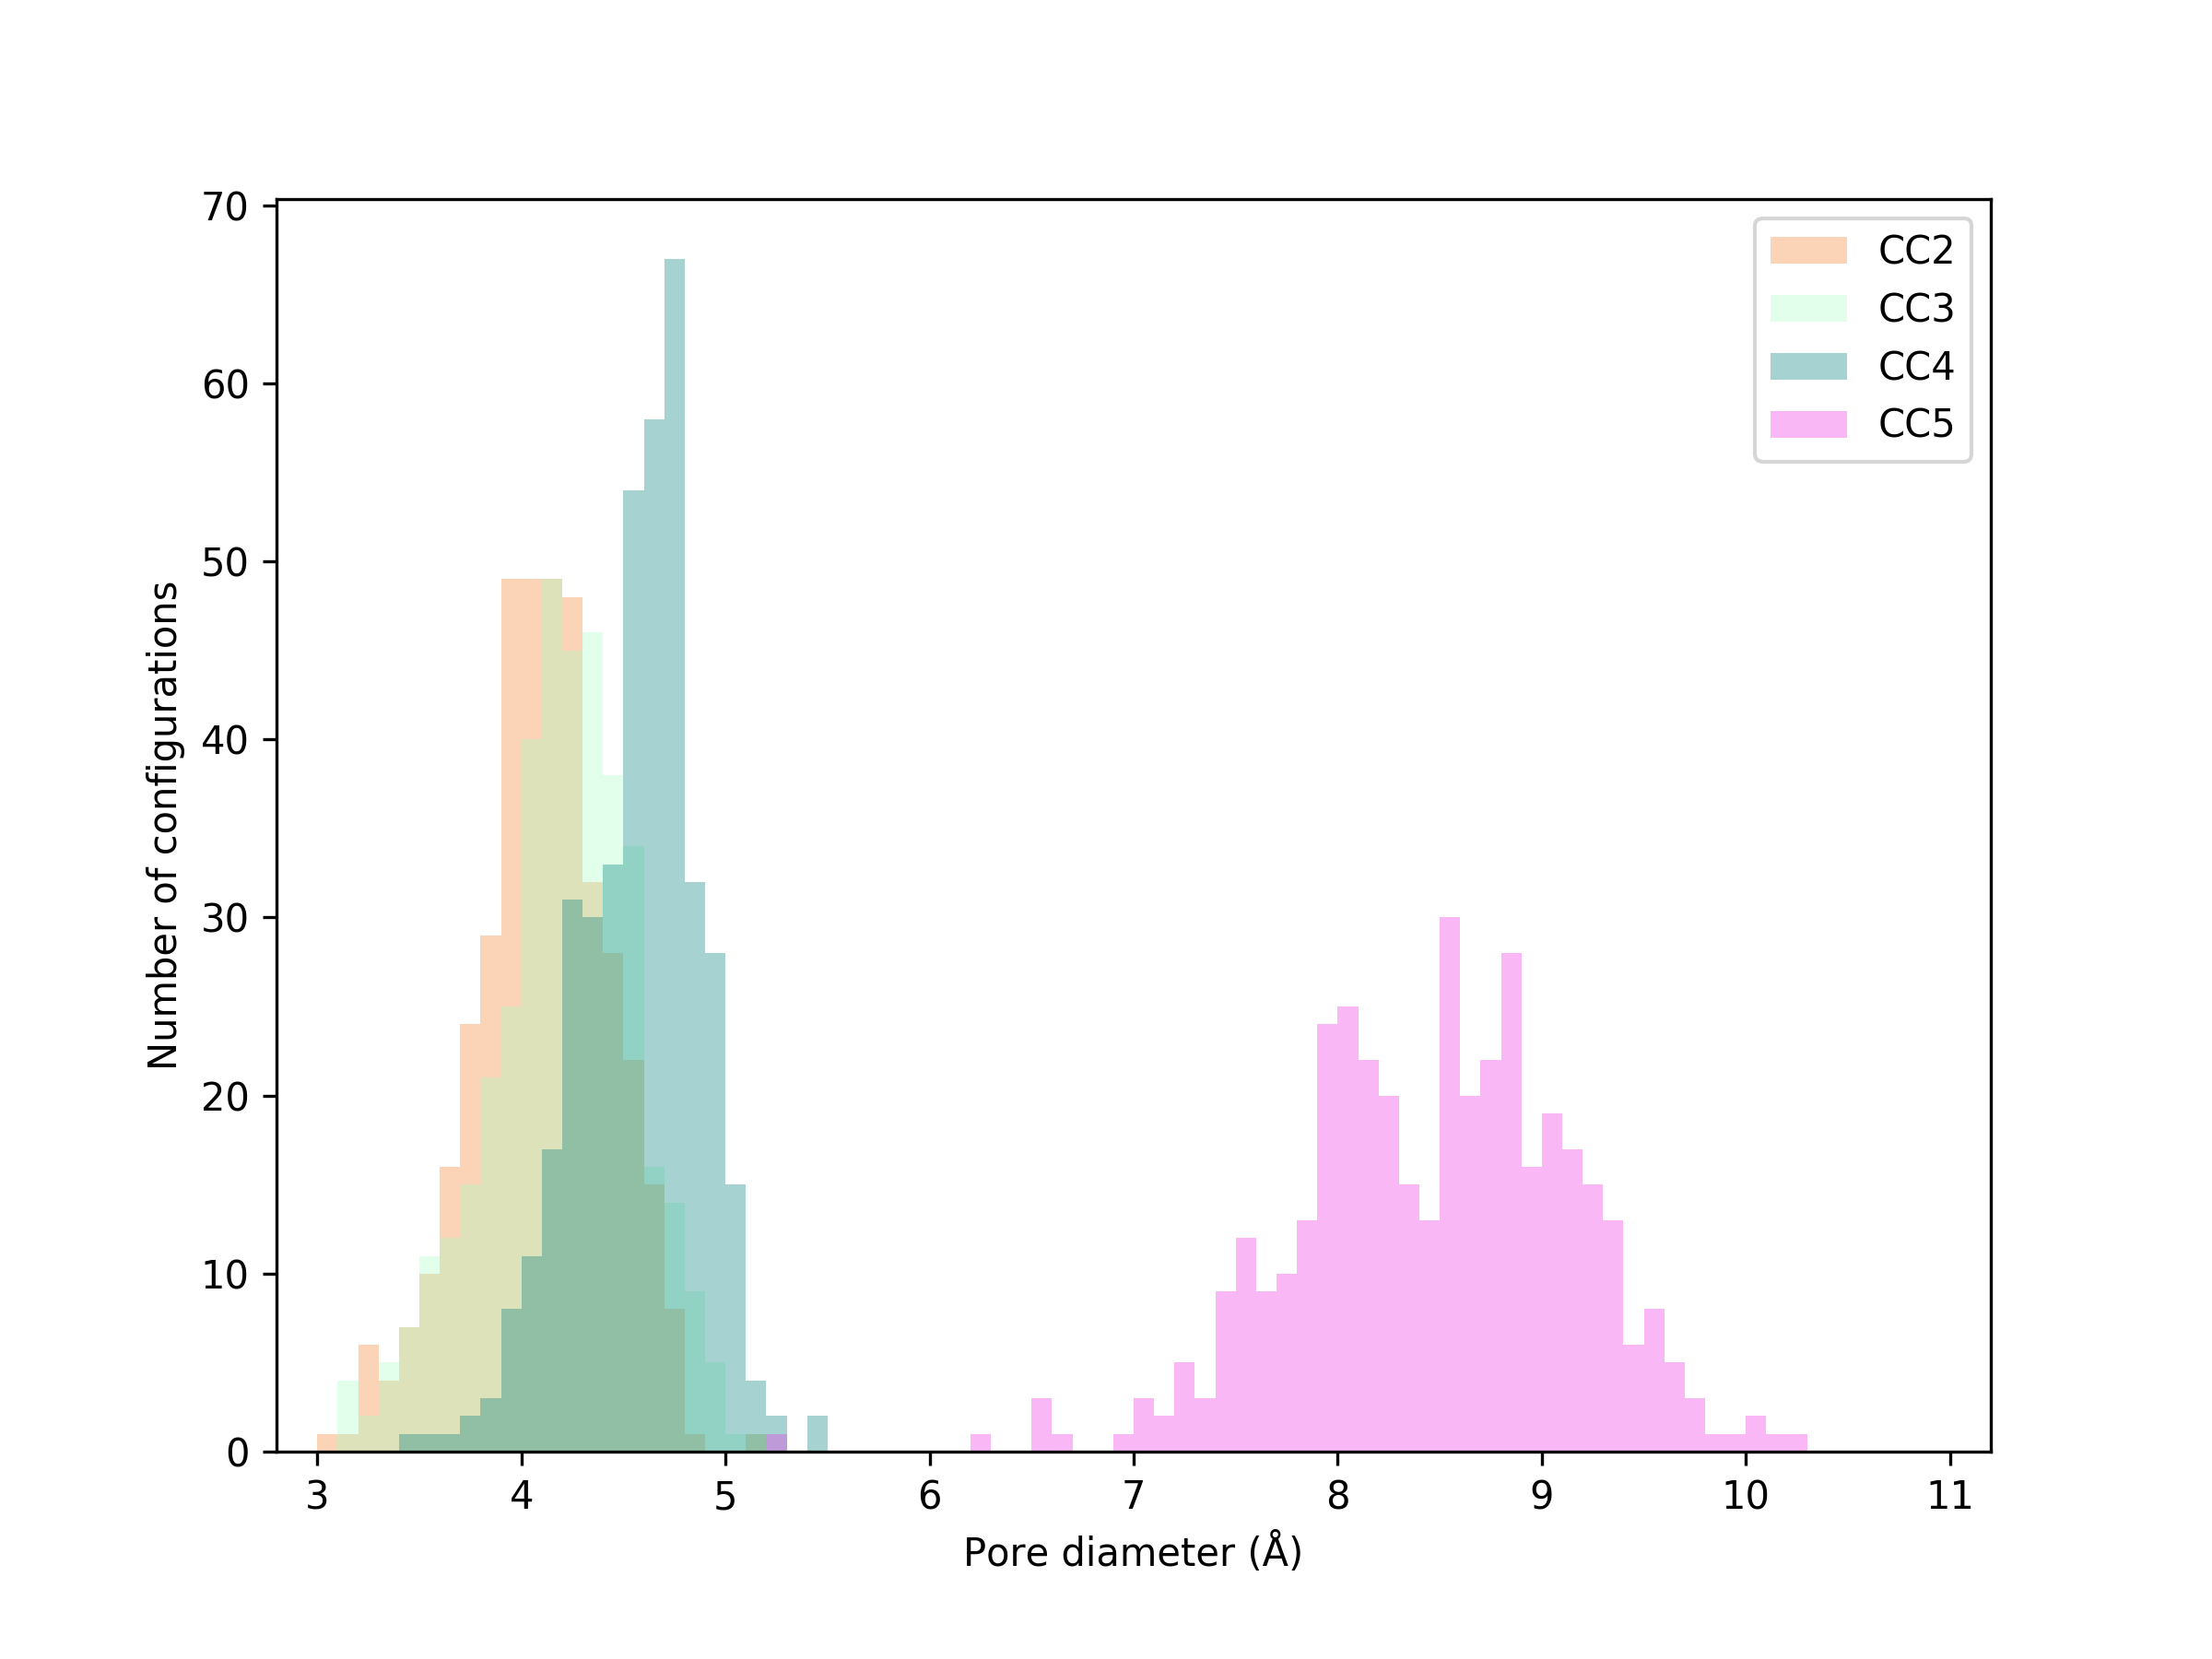
\includegraphics[width=0.65\columnwidth]{../pore_diameter_histogram.png}
	\caption{A histogram of the pore diameter, calculated using \texttt{pywindow}, exhibited by snapshots during the MD simulations. The colors denote the histograms for \textbf{CC2}, \textbf{CC3}, \textbf{CC4}, and \textbf{CC5}.
	} \label{fig:pore_diameter_histogram}
\end{figure}

Note that the region explored by the MD snapshots in Fig.~\ref{fig:pca_space_with_flex} does not overlap the latent representation of the rigid structure pulled from Miklitz et al. \cite{miklitz2017computational} (correspondingly colored solid point). The reason is that force field predicts a slightly different minimum-energy structure than the cage pulled from the Cambridge Structural Database by Miklitz et al. \cite{miklitz2017computational}. Regardless, Fig.~\ref{fig:pca_space_with_flex} provides valuable insight, showing how flexible cages explore regions of latent space as their cavity fluctuates.
%Talk about how the fluctuation might be different if solvent is within the pore? Static/Dynamic 

\clearpage

\section{Exploring accessibility of cages to xenon}
\label{sec:inaccessibility}

During the Henry coefficient calculations, we insert xenon atoms at random positions within a simulation box encompassing the cage molecule (see Sec.~\ref{sec:henrydetails}). These simulations may insert a xenon atom internal to a cage cavity whose window is too small for xenon to enter. This is an undesirable scenario, since xenon could practically never diffuse into the cavity in practice, yet that inner cavity is contributing to the simulated Henry coefficient. Here, we determine which cages have cavities that are inaccessible to a xenon or krypton atom.

To assess if an adsorbate can enter through a window into the cavity of the porous organic cages, we superimposed a grid of points over each cage molecule such that the distance between each adjacent datapoint was $0.1$ \AA. The potential energy of the adsorbate (xenon, krypton) was calculated at each point using a 12-6 Lennard Jones potential. Force field parameters were taken from the Universal Force Field (UFF) and geometric mixing rules were applied (14 $\angstrom$ cutoff). After the potential energy grid was computed, we assigned an integer value to each point, $-1$ if the energy was above a certain energy value (here $15 \ k_BT$ where $k_\text{B}$ is the Boltzmann constant and the temperature was taken to be $T = 298 \ \text{K}$), which corresponds to a non-occupiable point, and $1$ if the energy was below that value, corresponding to an occupiable point. The potential energy value $15k_B T$ is defined to be a potential energy barrier that is prohibitively high for xenon to occupy\cite{kim2012high}.
Next we see what occupiable points are connected. For every set of contiguously neighboring occupiable points, we relabel them unique values corresponding to a \emph{segment} of occupiable points by applying a flood fill algorithm \cite{martin2012accelerating,kim2012high}. If the center of the cage is occupiable \emph{and} belongs to a different segment than the region outside of the cage, we deem that cage's cavity as \emph{inaccessible}. If this were the case, the xenon adsorbate would have to overcome a prohibitively large energy barrier to percolate through the window and enter the cavity. This catches the undesirable case where Henry coefficients from the simulations have unrealistic contributions from the internal cage cavity despite the adsorbate being unable to percolate into the cavity because the window diameters are too small. In Fig.~\ref{fig:latent_space_S_Xe_Kr}, we mark this subset of cages with xenon-inaccessible cavities with an `x'.

This method was applied to all of the 74 rigid porous organic cages, not taking into consideration that the window can ``breathe''', i.e. fluctuate to allow the adsorbate to enter \cite{miklitz2017computational}. The set of cages deemed to harbor inaccessible cavities to xenon is in Table \ref{tbl:inaccessible}, where the inaccessible cages can be seen along with their maximum window diameter (calculated with \texttt{pywindow}). Note that these xenon-inaccessible cages have maximum window diameters less than the diameter of a xenon atom, which is c.a.\ 4 \AA, consistent with our method. 

Miklitz et al.\cite{miklitz2017computational} conducted a similar analysis where they used molecular dynamics (MD) to observe the pore breathing and calculated the distribution of pore-limiting envelopes (PLE) of the MD snapshots. Their dynamic PLE analysis of what percentage of the time cages have windows large enough for \ce{Xe} to percolate into the cavities contrasts with our method of focusing on a static cage structure and making a binary classification as accessible or inaccessible based on the potential energy barrier at the window. Of the subset of 12 cages they studied, \textbf{CP1} and \textbf{WC4} were the only two they identified as having cavities inaccessible to xenon practically for all of the time (0.2\% of the time); our analysis identifies \textbf{CP1} and \textbf{WC4} as inaccessible as well. A notable exception was \textbf{RCC3a}, which was open only 1.1\% of the time in their MD simulations, but, according to our analysis, is accessible. A possible source of discrepancy is that the force field used in the MD simulations of Miklitz et al.\cite{miklitz2017computational} may provide a different ``average'' structure than deposited in the Cambridge Structural Database (the source of our \textbf{RCC3a} structure from Ref.\cite{miklitz2017computational}). Other cages such as \textbf{CC3}, \textbf{CC2} and \textbf{NC2} were open to \ce{Xe} roughly $10 \%$ of the time, considered accessible as in our analysis. 

\begin{table}
  \caption{A list of the cages found to be inaccessible to xenon alongside their maximum window diameter (calculated with \texttt{pywindow}).}
  \label{tbl:inaccessible}
  \begin{tabular}{cc}
    \hline
    \textbf{Cage}  & \textbf{Maximum window diameter [\AA]}  \\
    \hline
    CB5 & $2.334$ \\
    CP1 & $2.392$ \\
    CP3 & $2.679$ \\
    CP4 & $1.495$ \\
	CP5 & $1.474$ \\
    HC1 & $3.594$ \\
    RCC1a & $2.016$ \\
    RCC1b & $2.180$ \\
    RCC1c & $2.786$ \\
	RCC1d & $2.578$ \\
	WC2 & $2.682$ \\
	WC3 & $1.578$ \\
	WC4 & $3.281$ \\
    \hline
  \end{tabular}
\end{table}

\clearpage
\newpage


\section{Adsorption site analysis}
Here, we analyze the distribution of adsorption sites of xenon internal and external to the cavity of the cage molecules. We consider any local minimum in the potential energy as a potential adsorption site. We identified potential energy minimia on the basis of a computed potential energy grid as in Sec.~\ref{sec:inaccessibility}. We looked at the 3D array storing the potential energy grid, looped over each element, and, if no lower values were adjacent to it, stored it as a local minimum. All local minima exhibiting positive energy values (repulsive) were discarded. 
Fig.~\ref{fig:energy_vs_dist} shows each local energy minimum as a point; the $y$-axis is the value of the potential energy at the local minimum and the $x$-axis is its distance from the center of mass of the cage. For reference, we plotted as a vertical line the radius of the cavity, computed by taking the 2-norm of the vector between the center of mass of the cage and the closest atom and correcting it with the van der Waals radius of the closest atom. This allows us to assess the relative potential energies of the adsorption sites internal to the cavity versus on the periphery or window site of the molecule.

\begin{figure}
\centering
	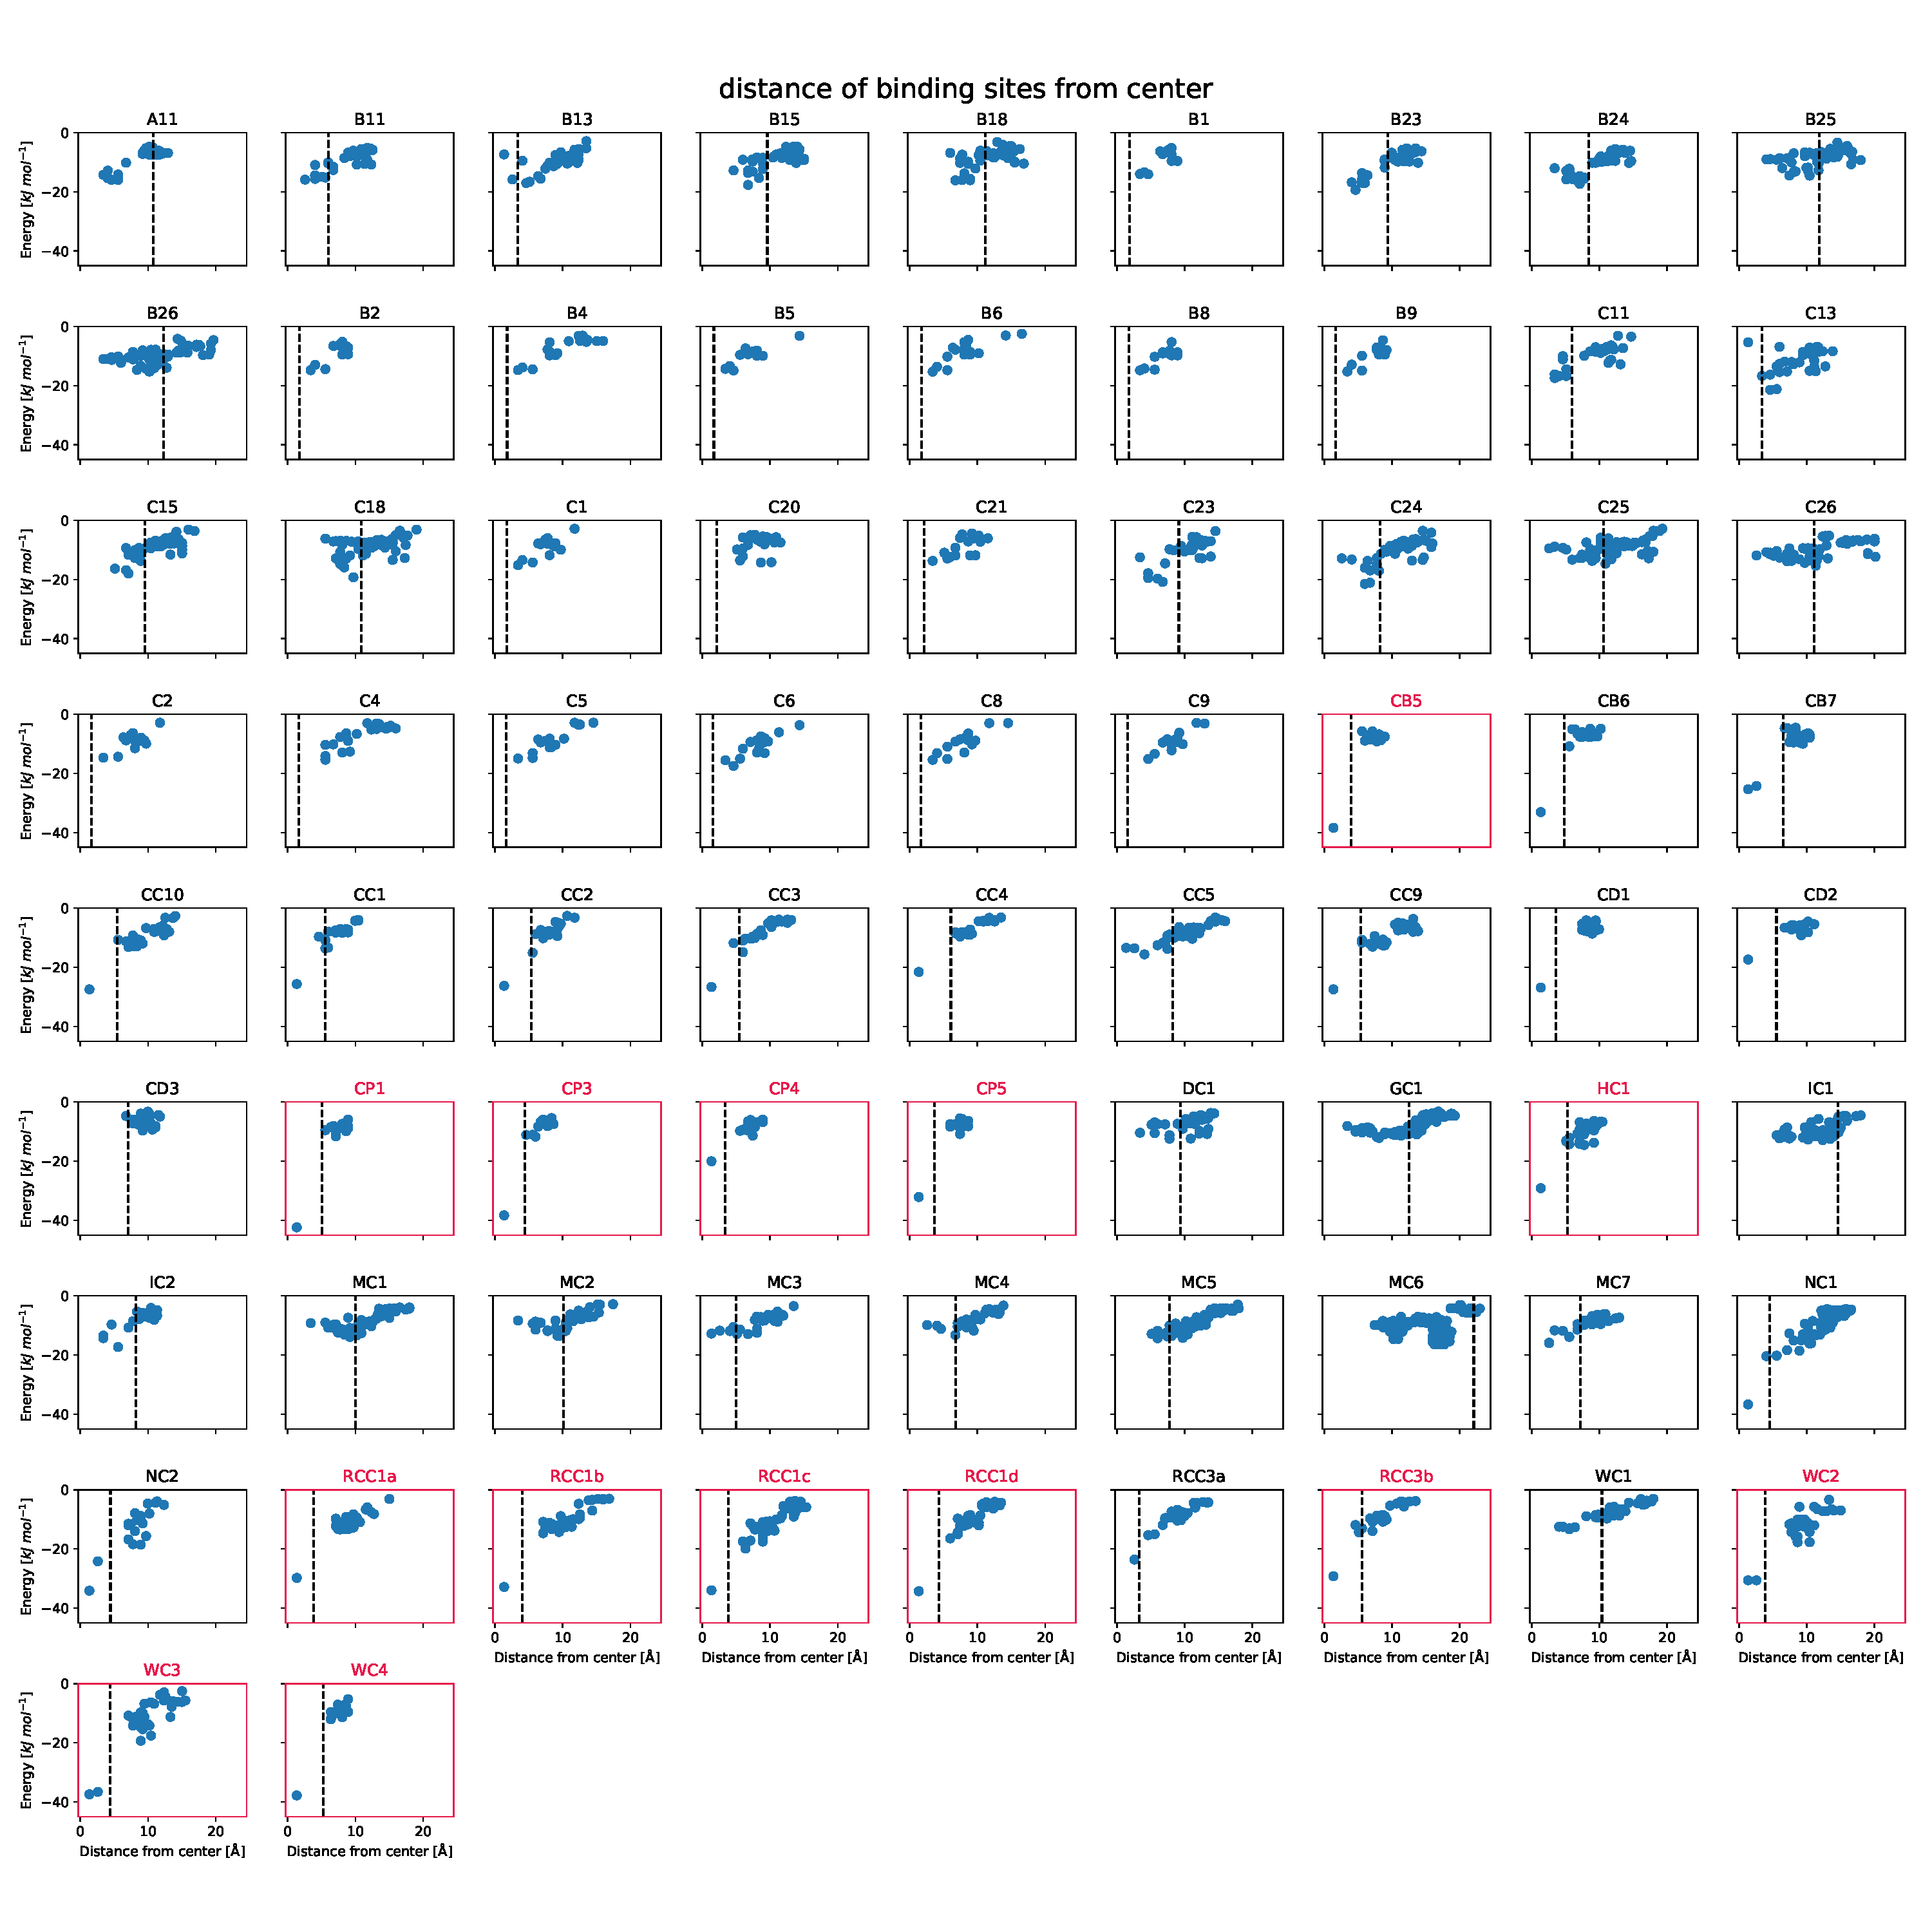
\includegraphics[width=\columnwidth]{../distance_of_binding_sites.pdf}
	\caption{Energy of each local potential energy of xenon minima [kJ mol$^{-1}$] plotted against the distance from the center of mass of each cage [\AA]. The red frames correspond to the cages deemed inaccessible by our flood fill algorithm. The cavity diameter is plotted as a vertical, dotted line to give an idea of the relative potential energies of adsorption sites within the cavity versus on the periphery or window site of the cage.
	} \label{fig:energy_vs_dist}
\end{figure}

\clearpage

% see viz.ipynb
\section{Visualization of the cage structures}
Larger images of the cages in Fig.~\ref{fig:cages} are shown in Fig.~\ref{fig:allcagesdetailed}.
\captionsetup[subfigure]{labelformat=empty} % get rid of a b c d
\begin{figure}[!h]
\centering
\subfloat[A11]{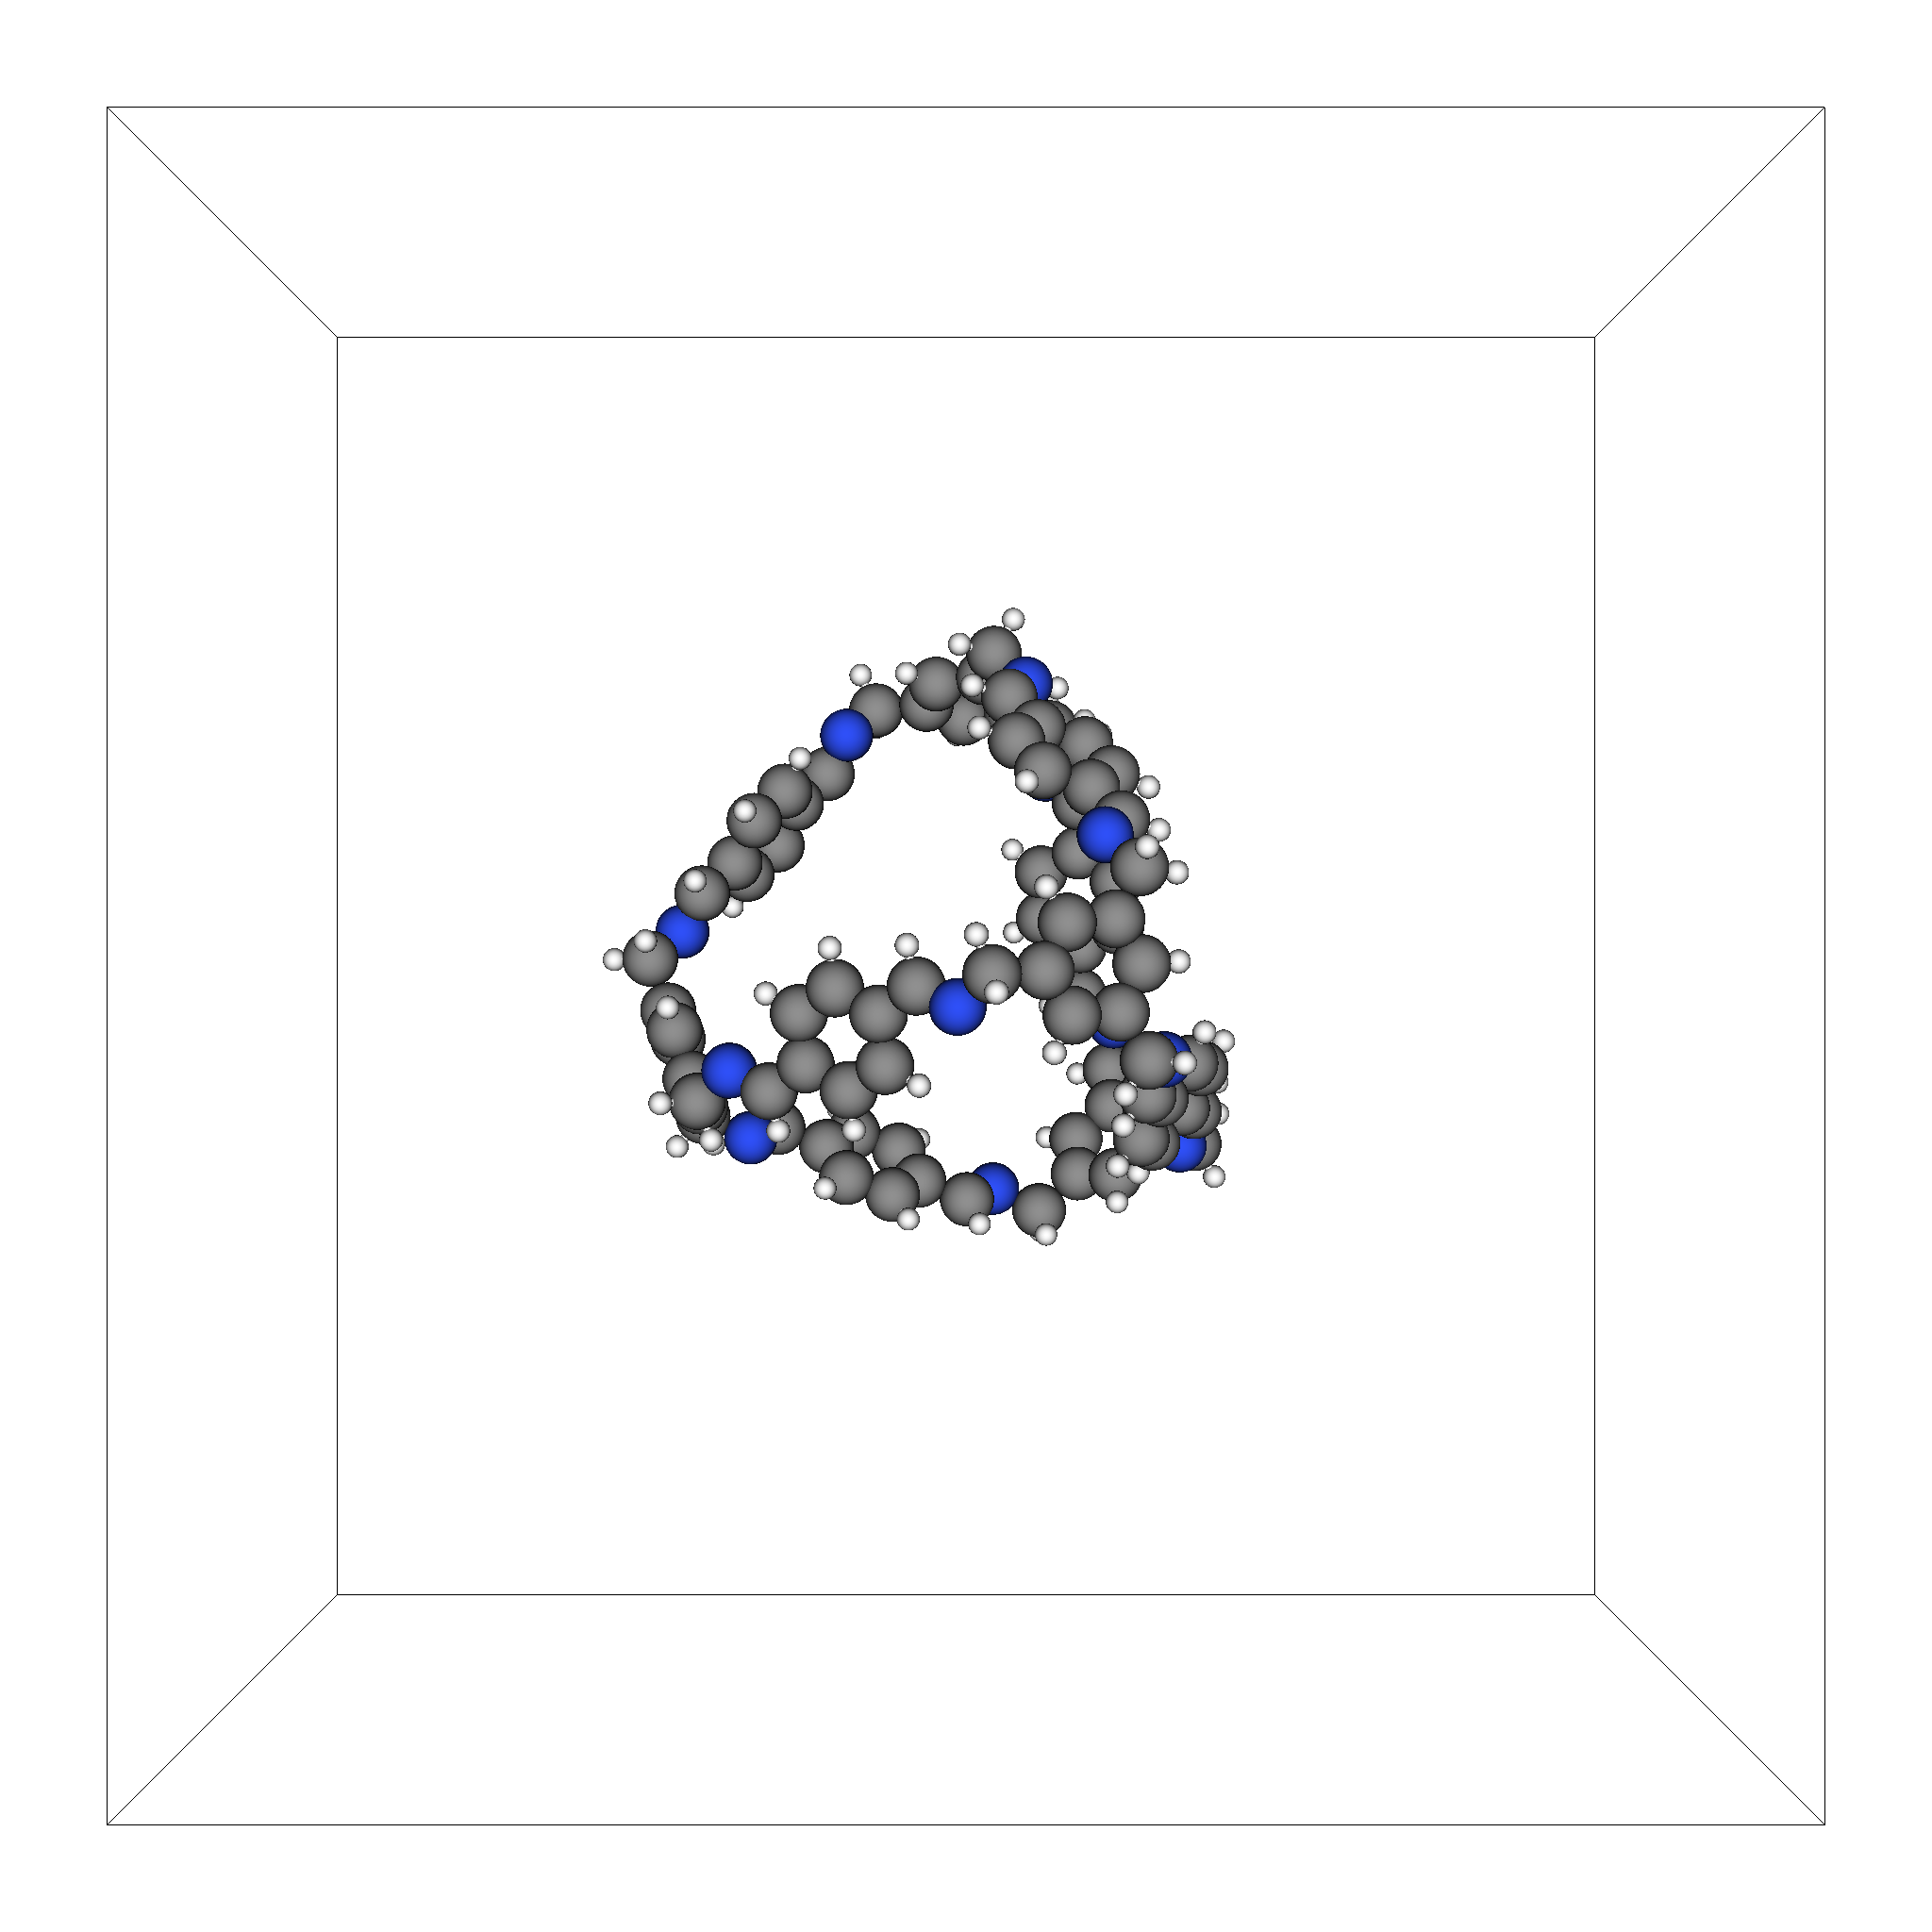
\includegraphics[width=0.25\columnwidth]{../final_aligned_cages/A11.png}}
\subfloat[B11]{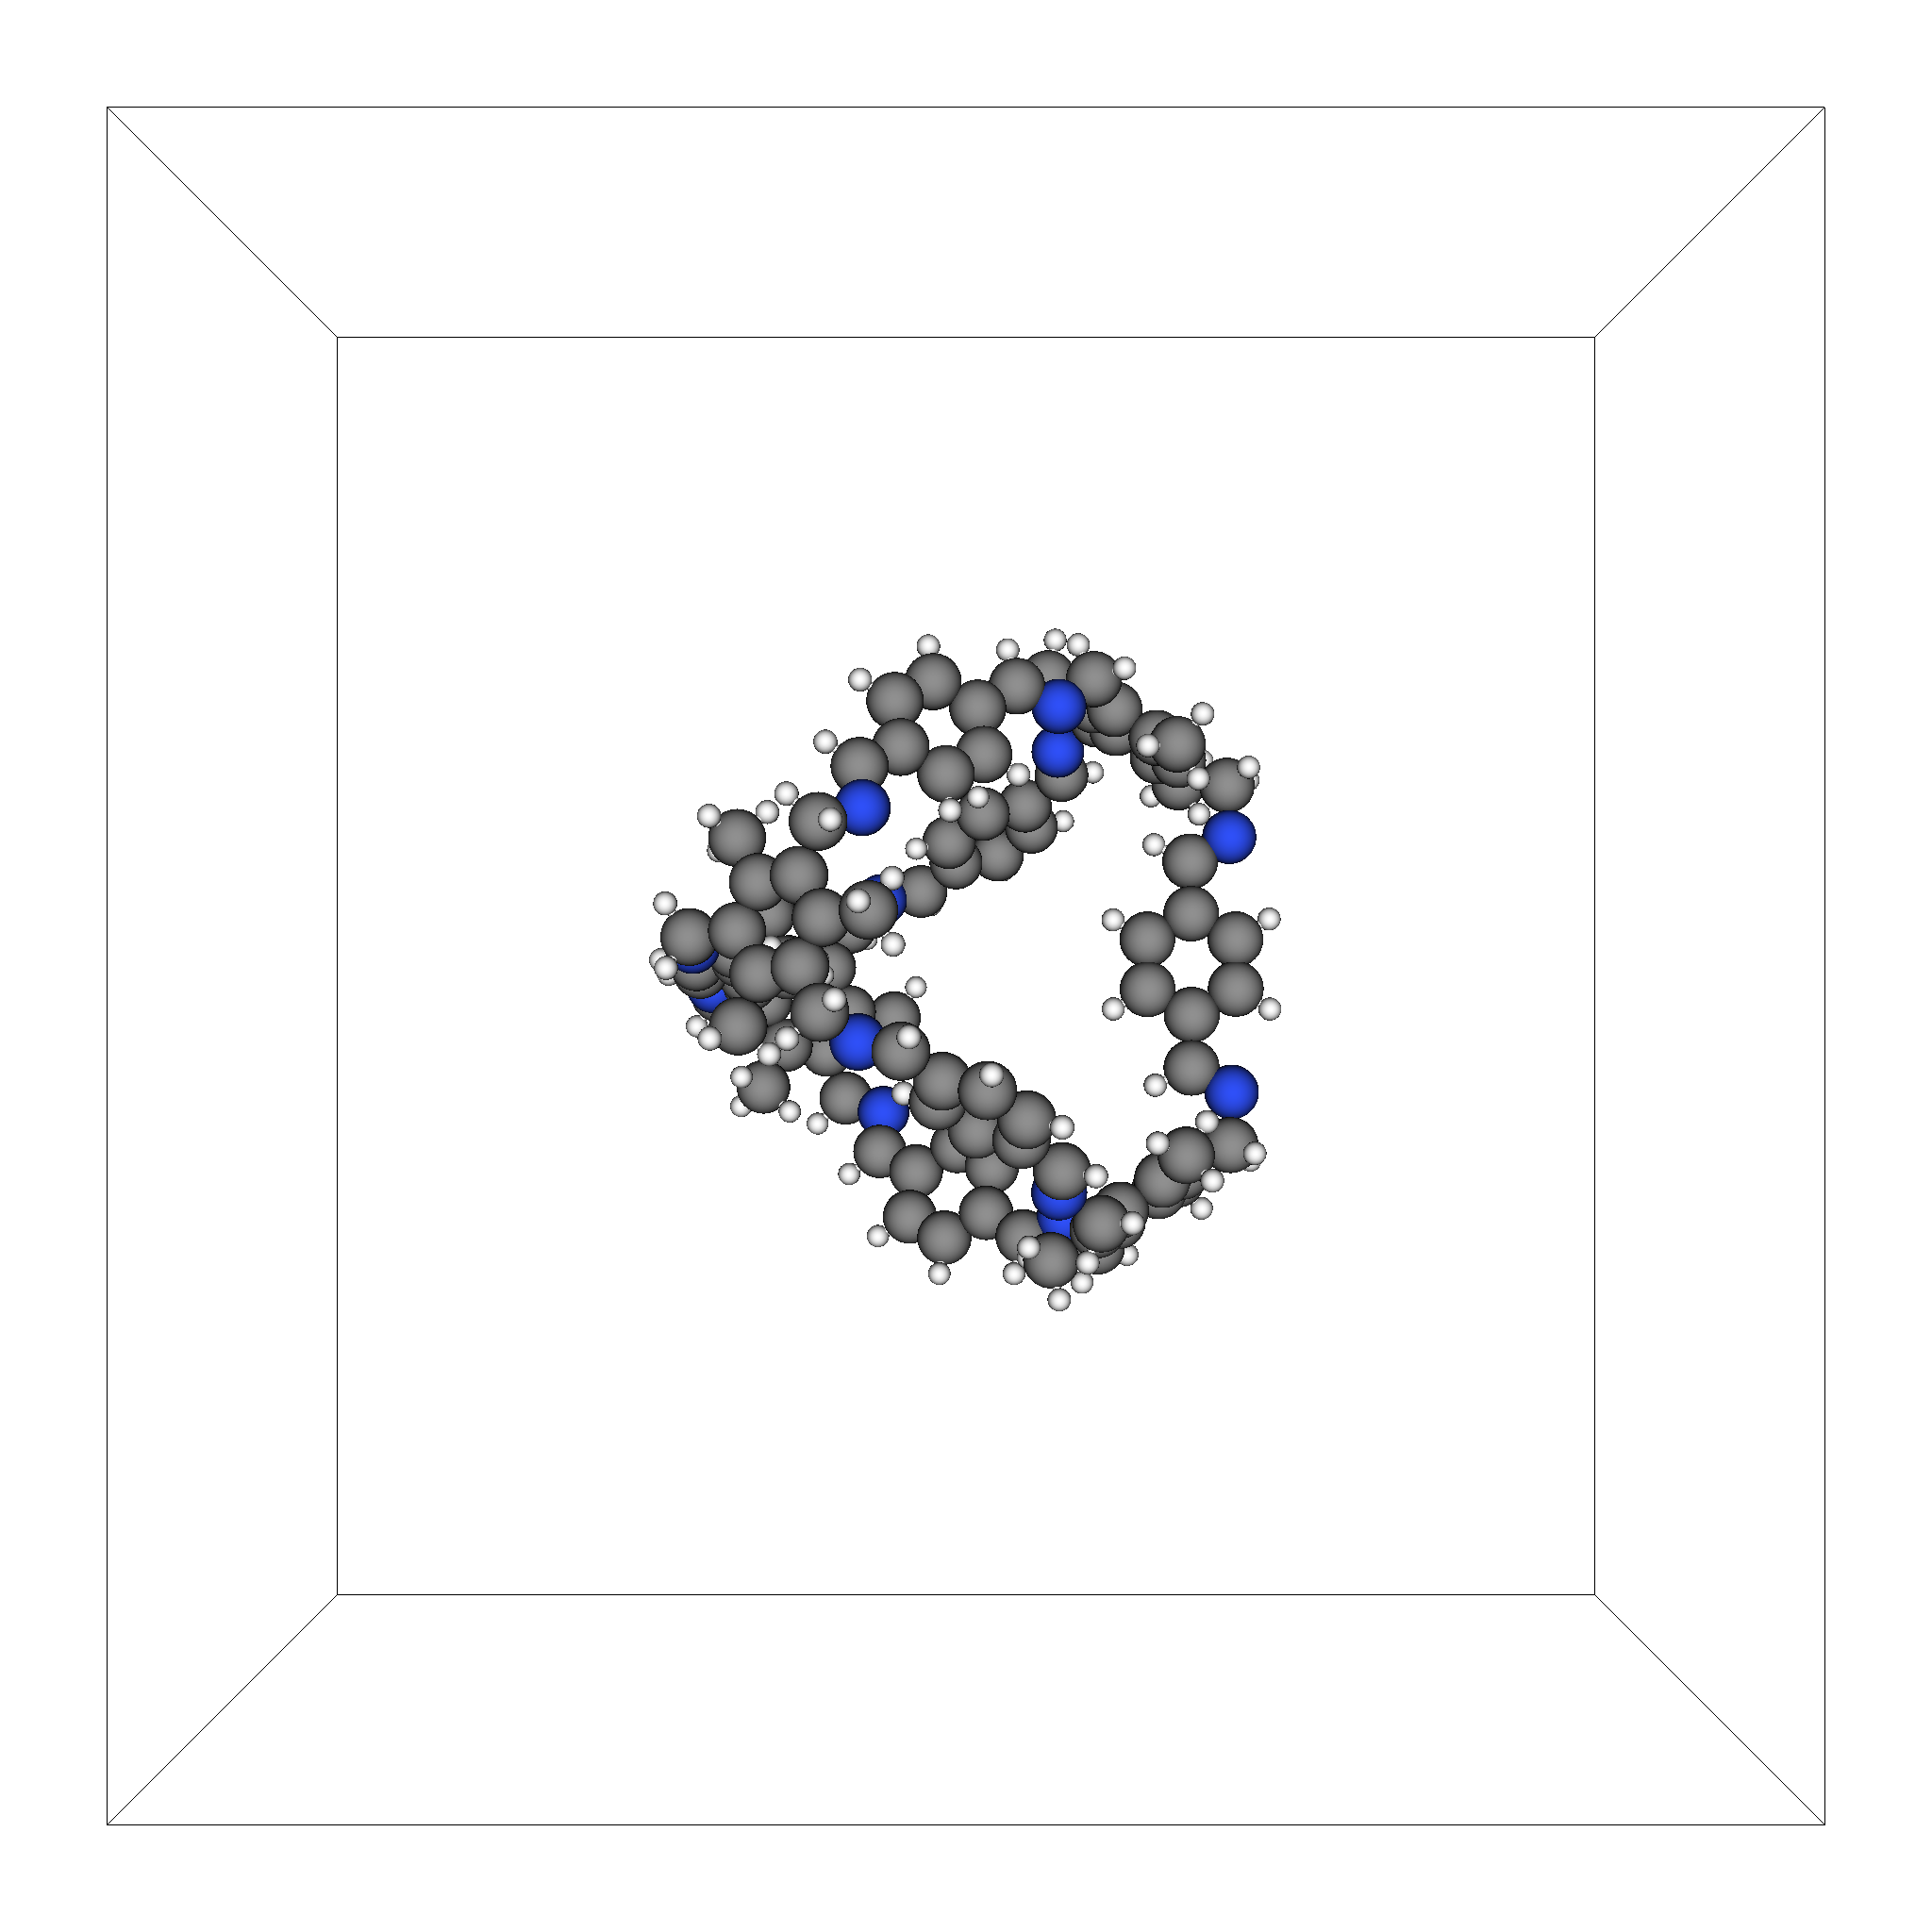
\includegraphics[width=0.25\columnwidth]{../final_aligned_cages/B11.png}}
\subfloat[B13]{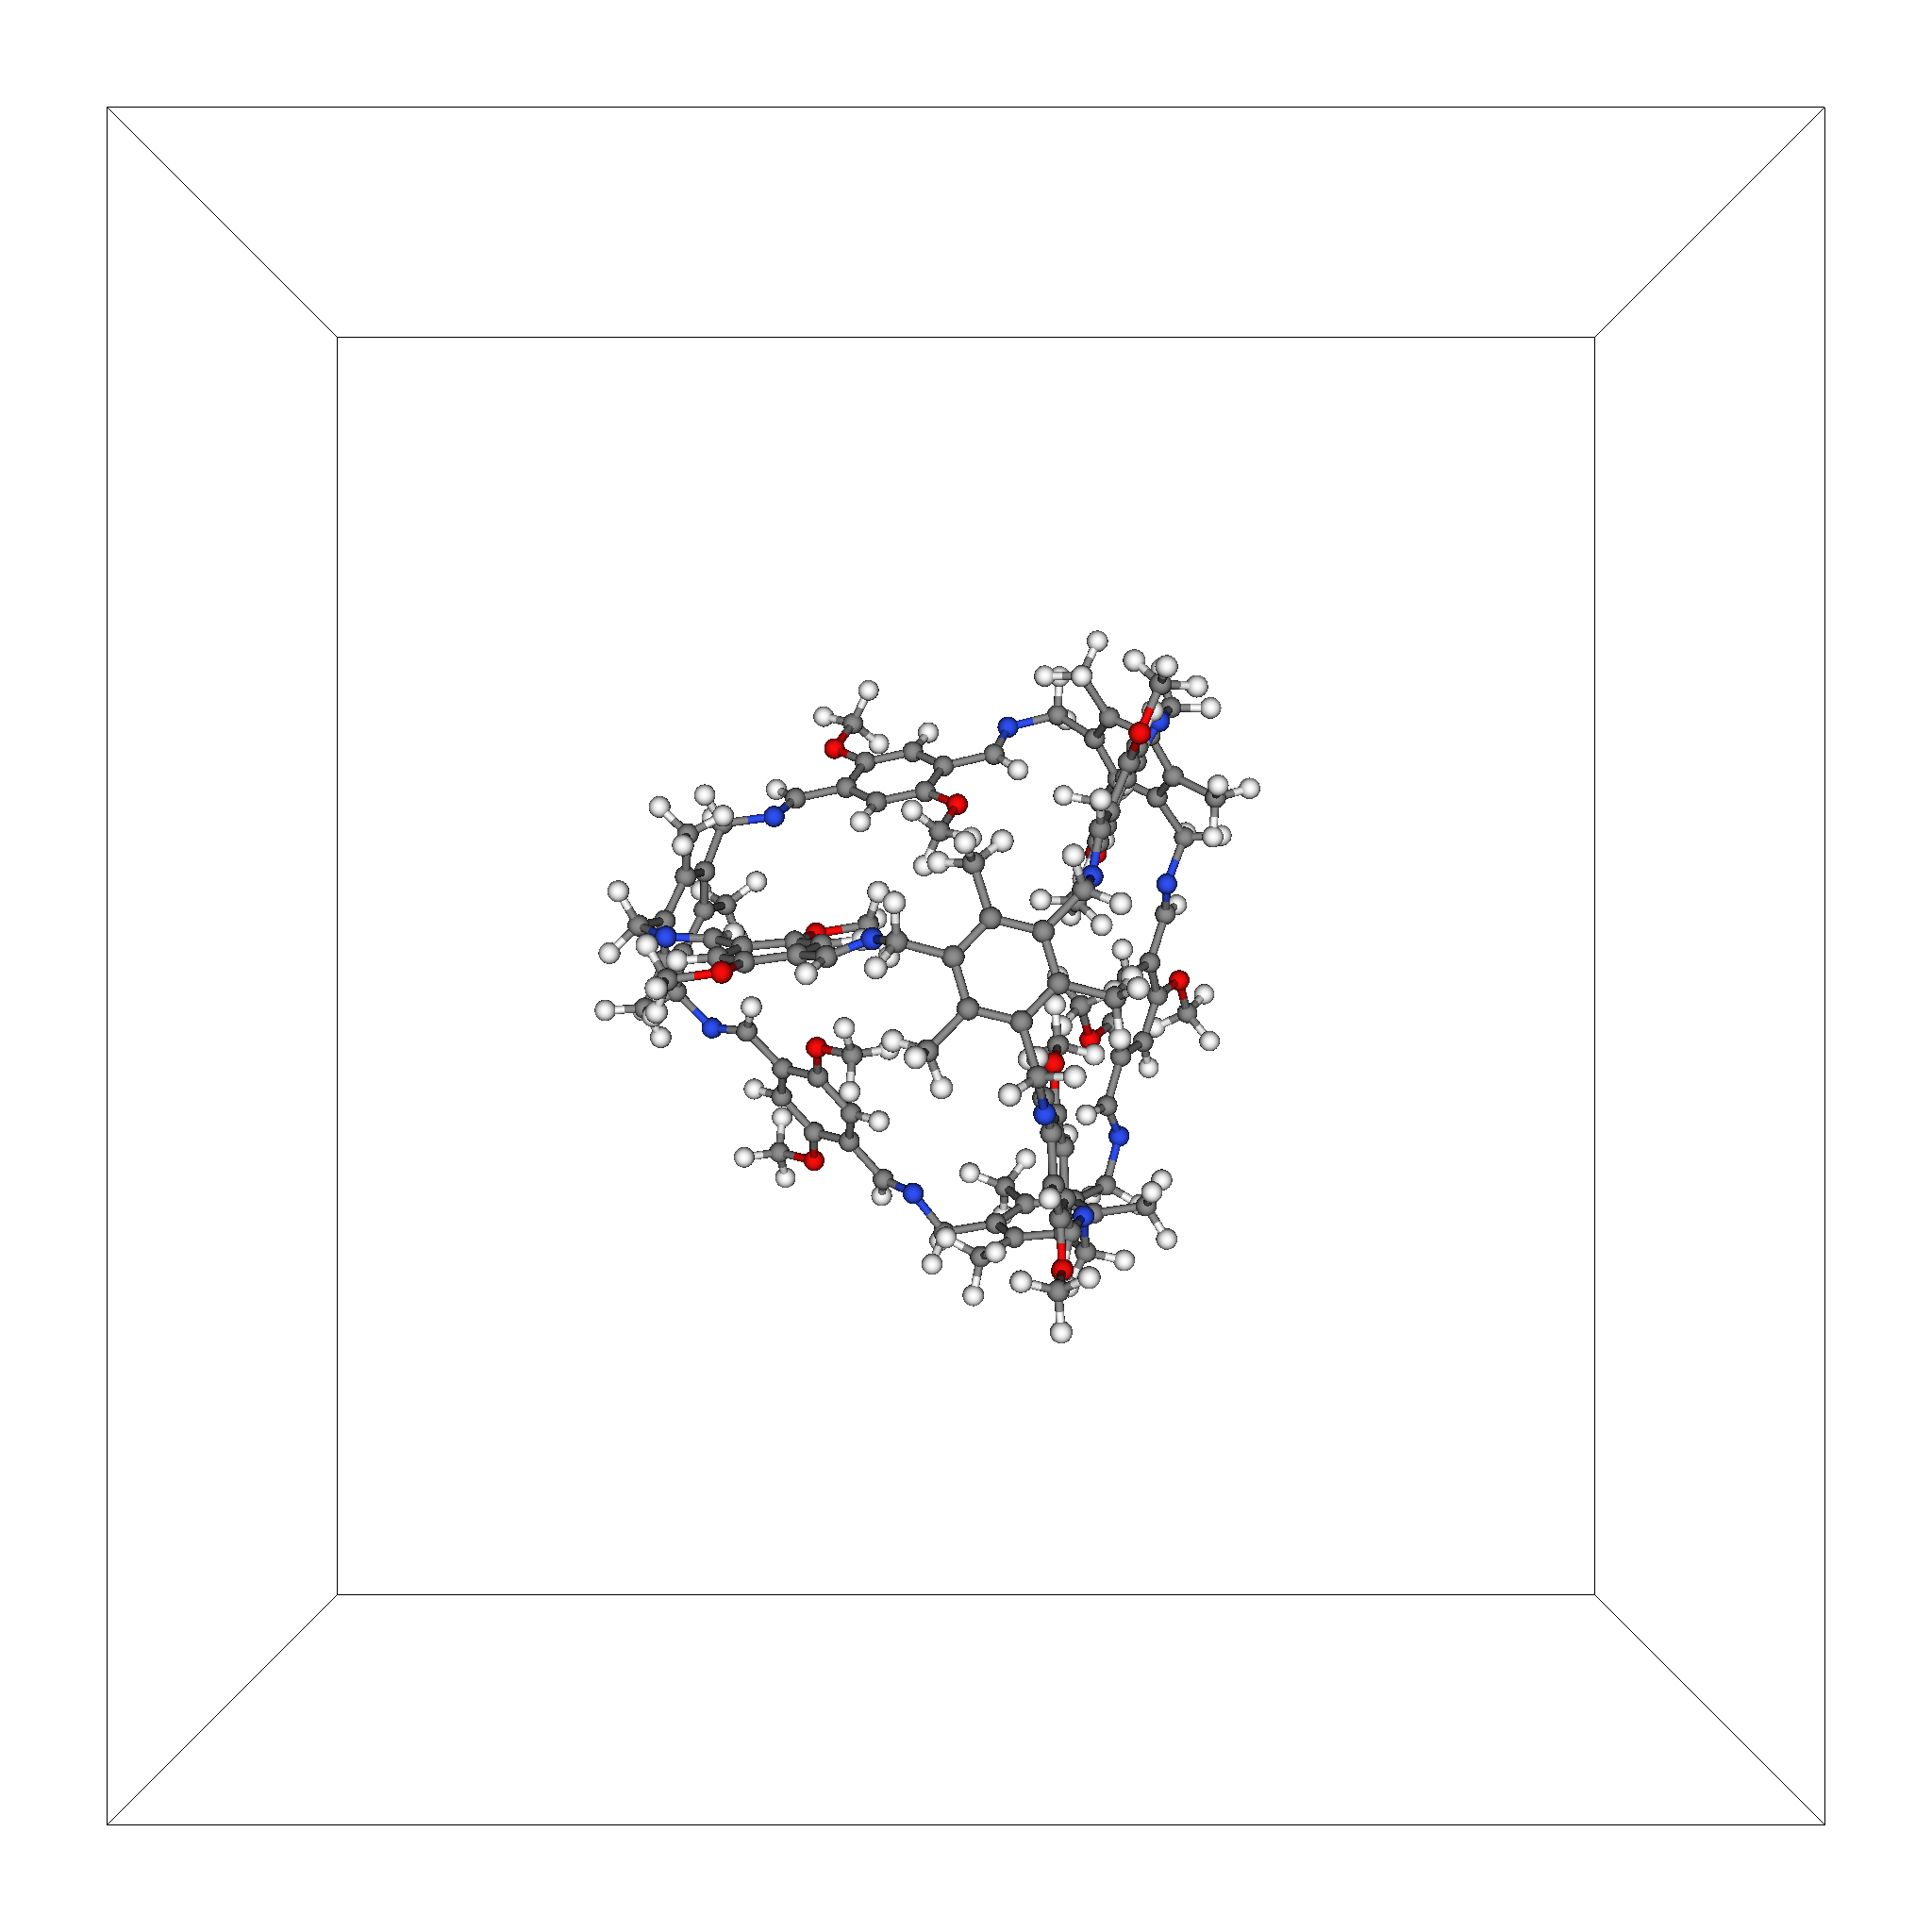
\includegraphics[width=0.25\columnwidth]{../final_aligned_cages/B13.png}}
\qquad
\subfloat[B15]{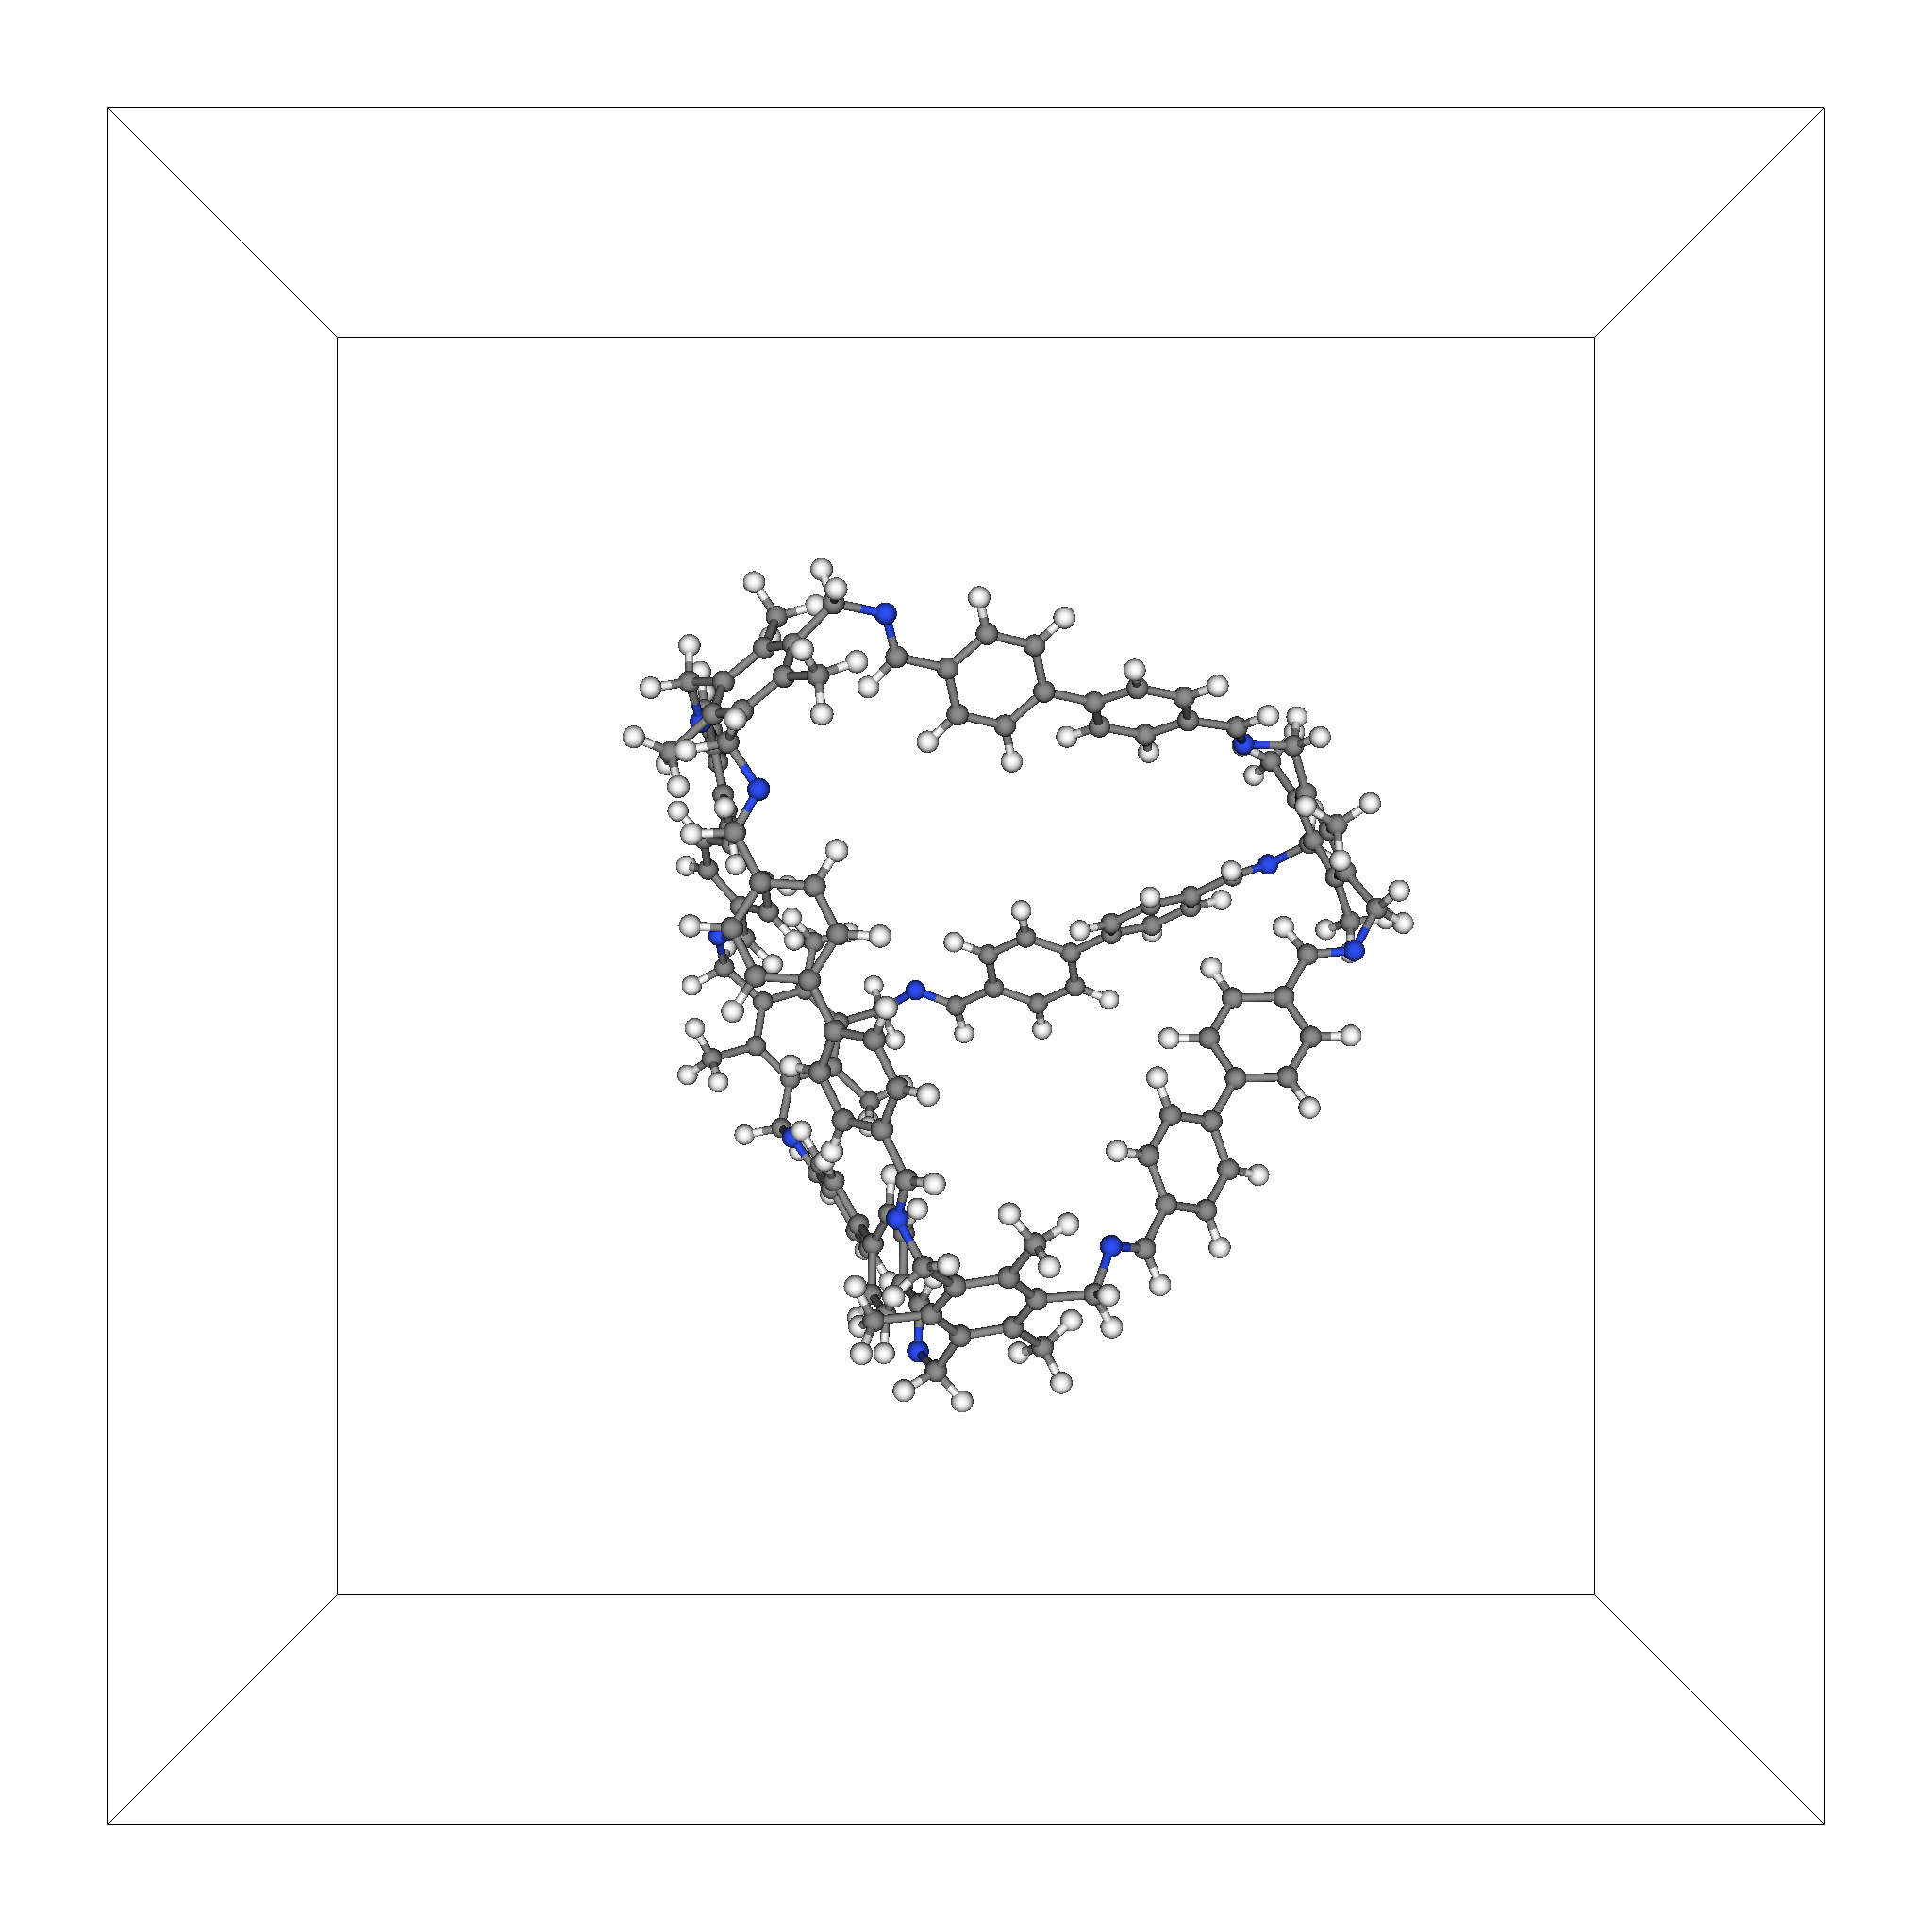
\includegraphics[width=0.25\columnwidth]{../final_aligned_cages/B15.png}}
\subfloat[B18]{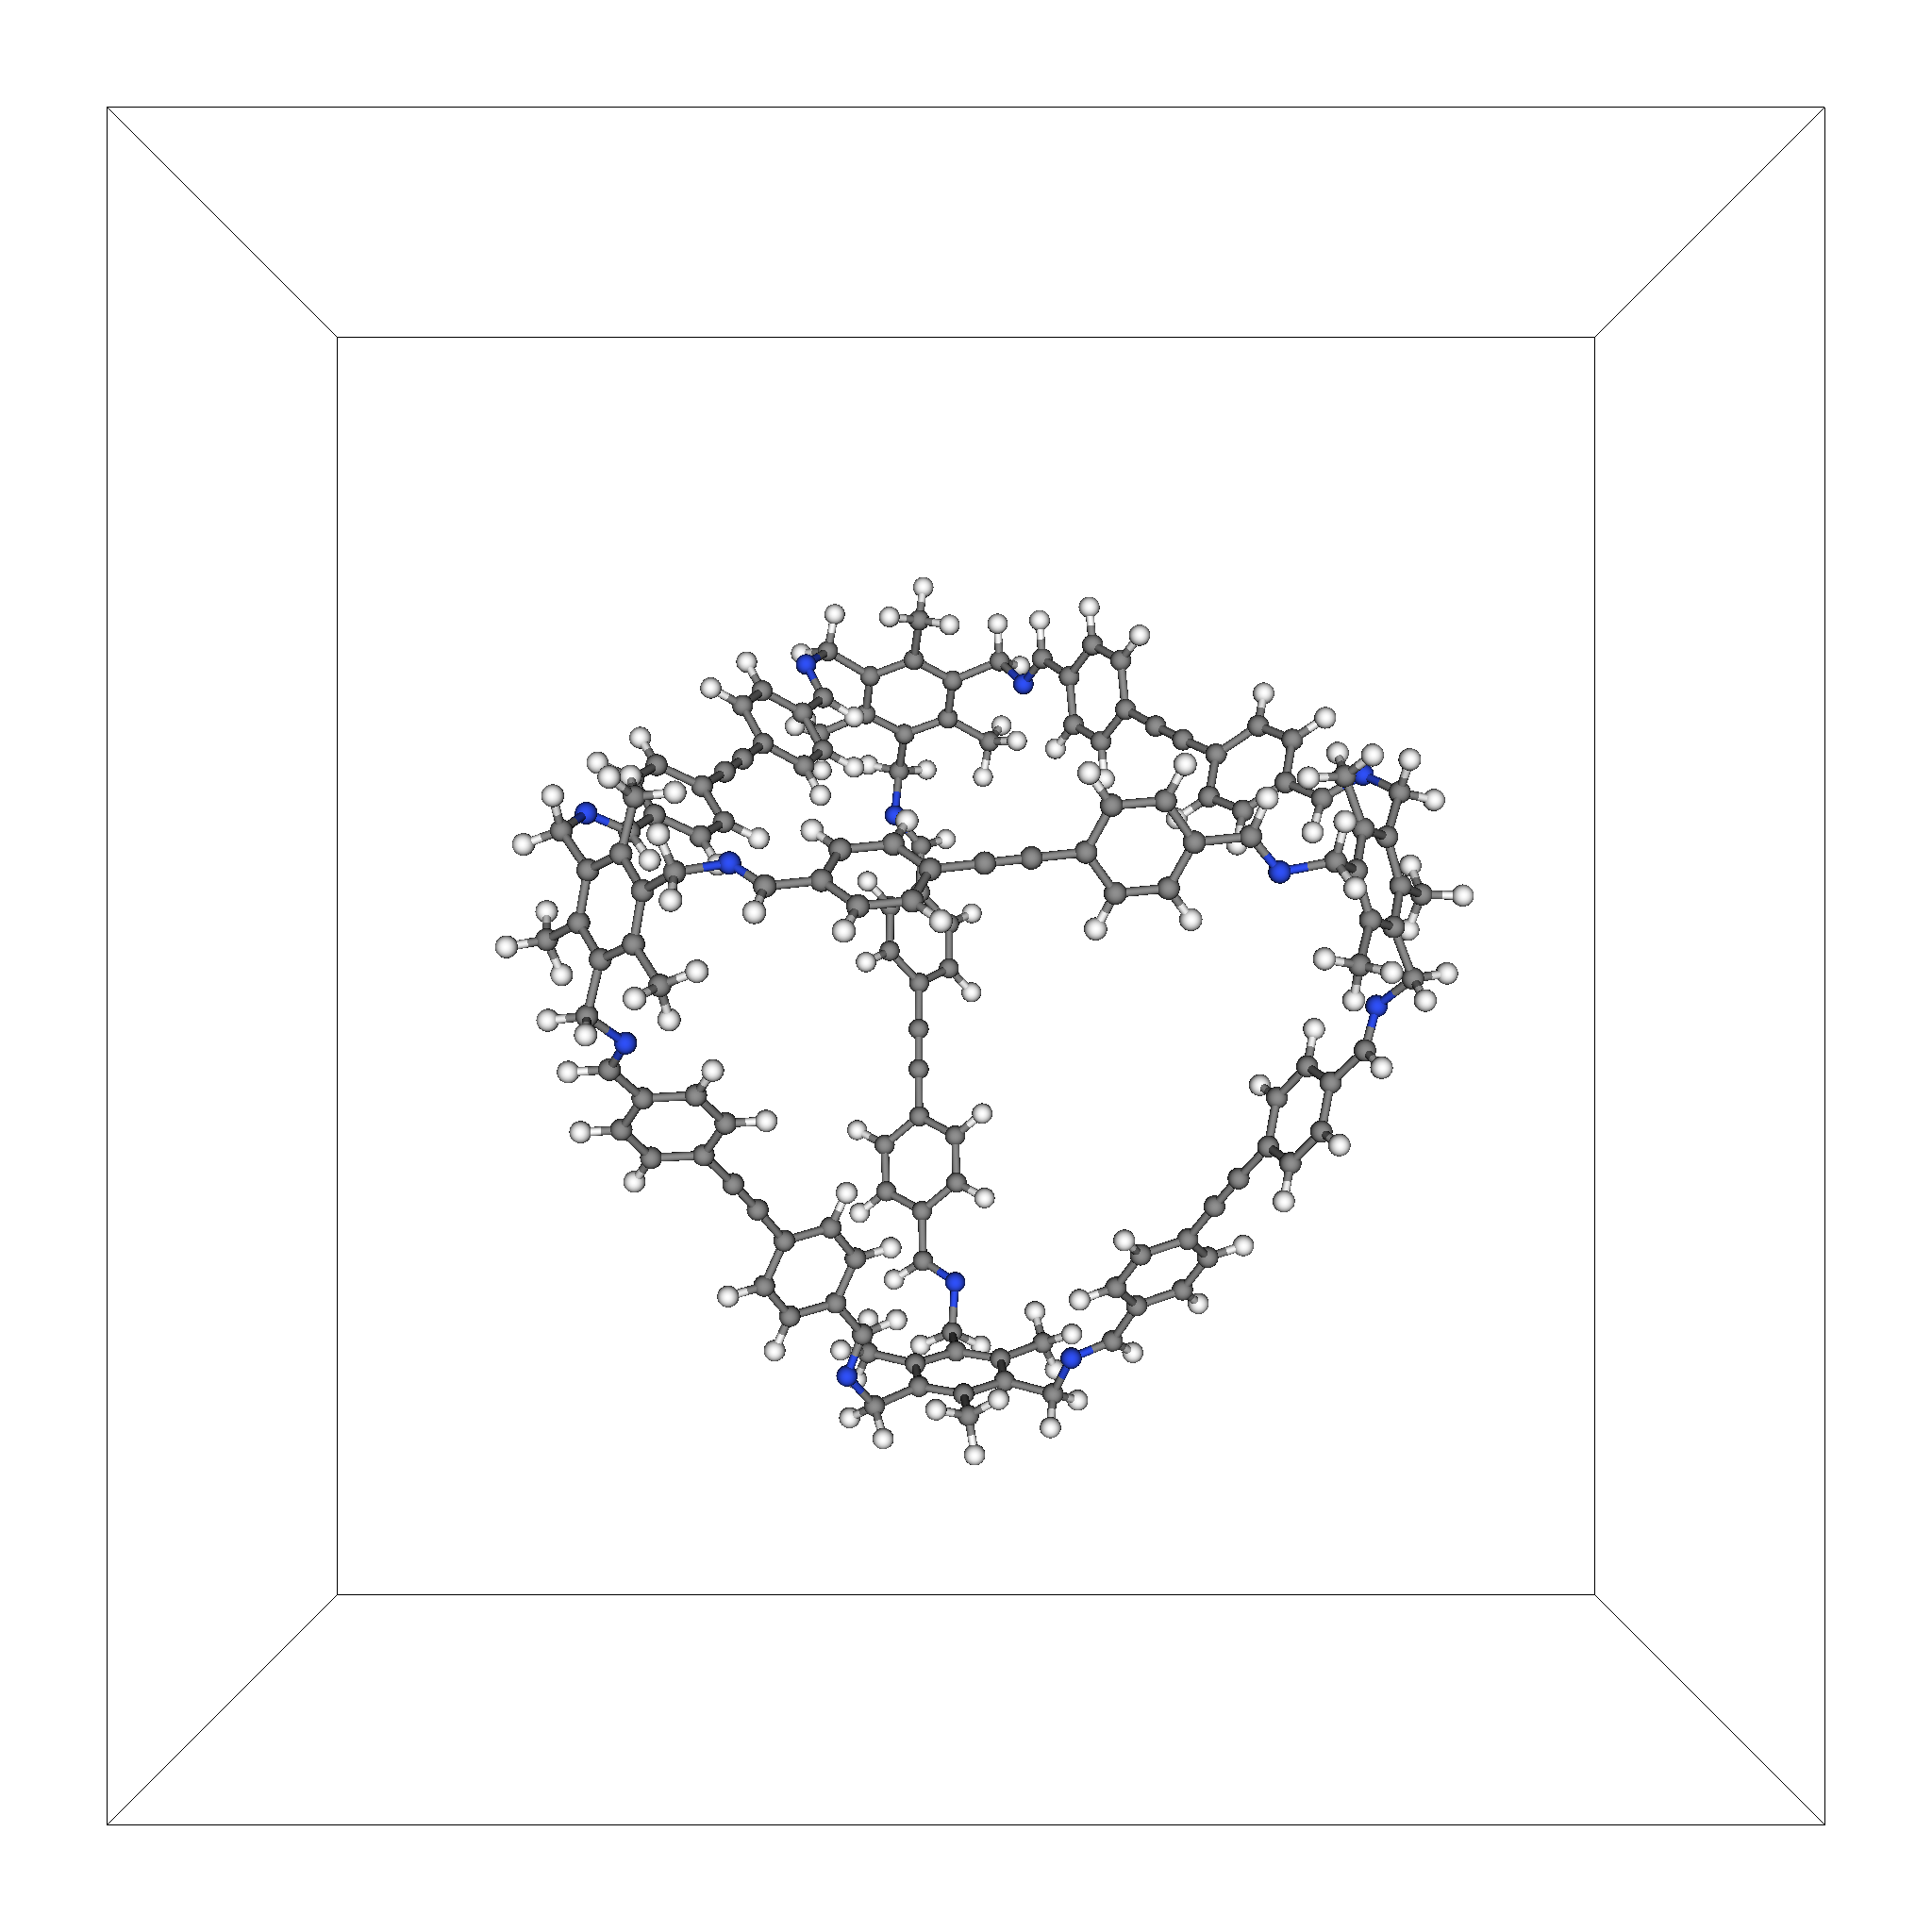
\includegraphics[width=0.25\columnwidth]{../final_aligned_cages/B18.png}}
\subfloat[B1]{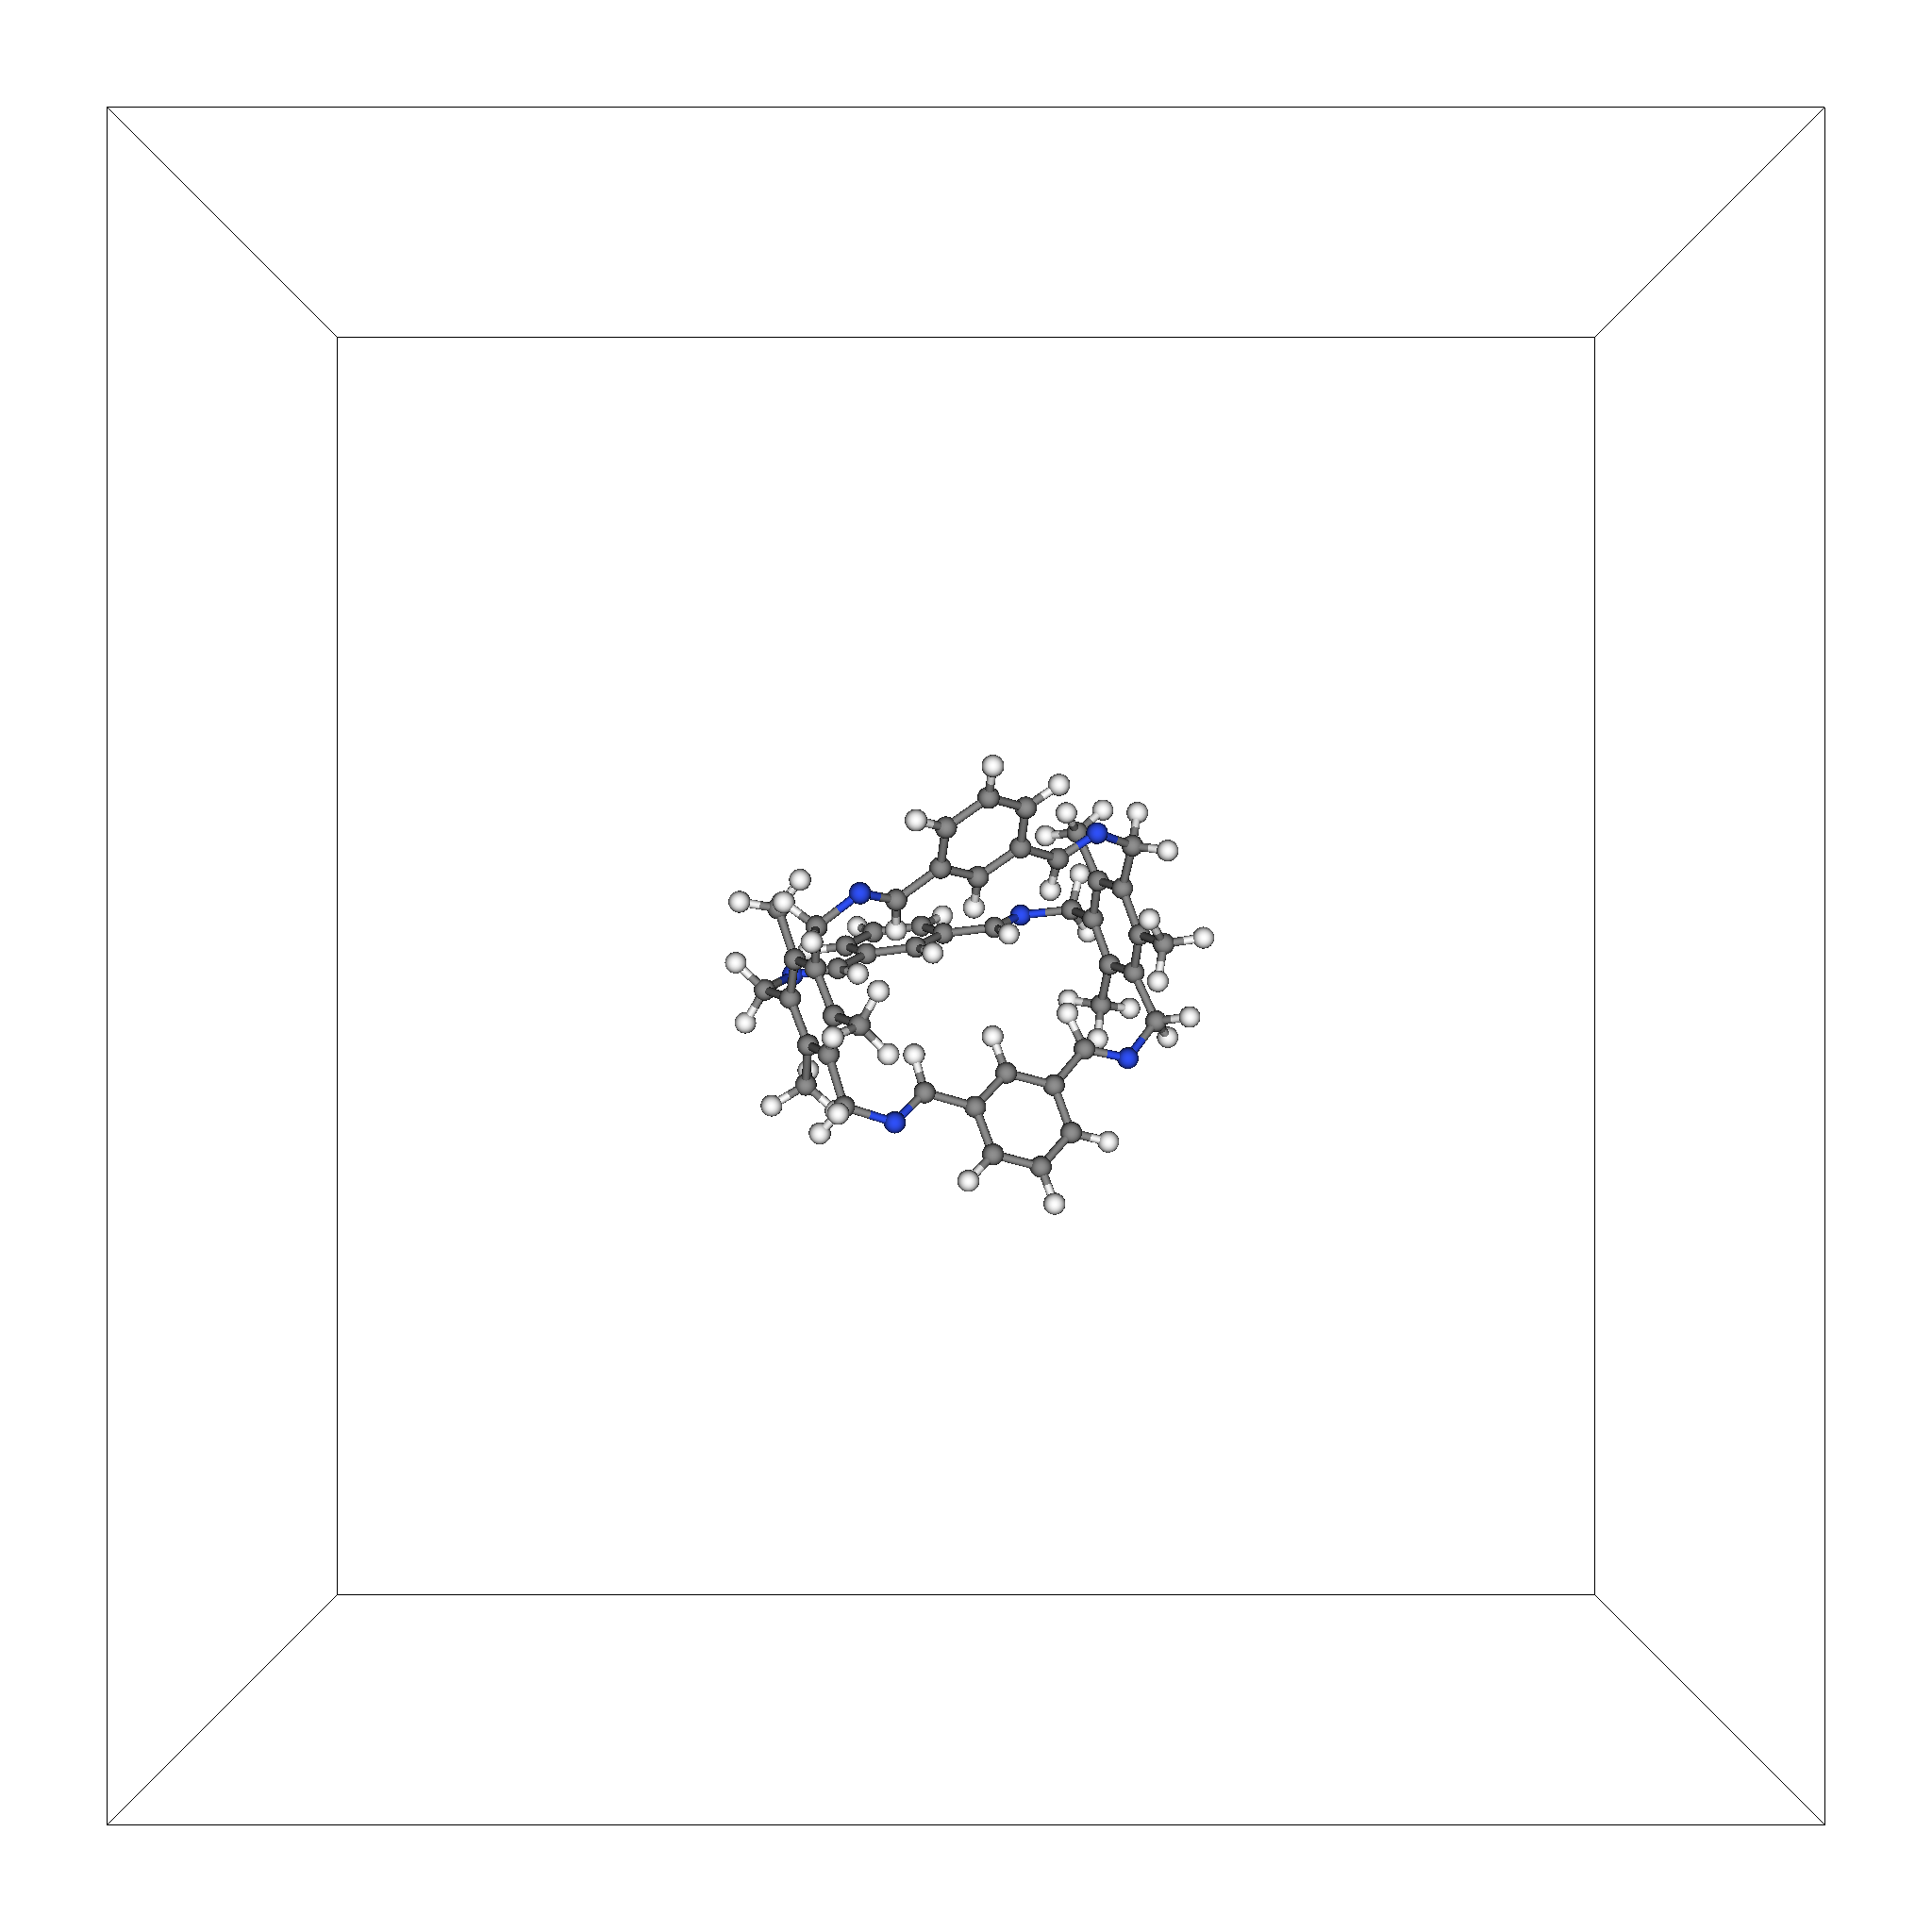
\includegraphics[width=0.25\columnwidth]{../final_aligned_cages/B1.png}}
\qquad
\subfloat[B23]{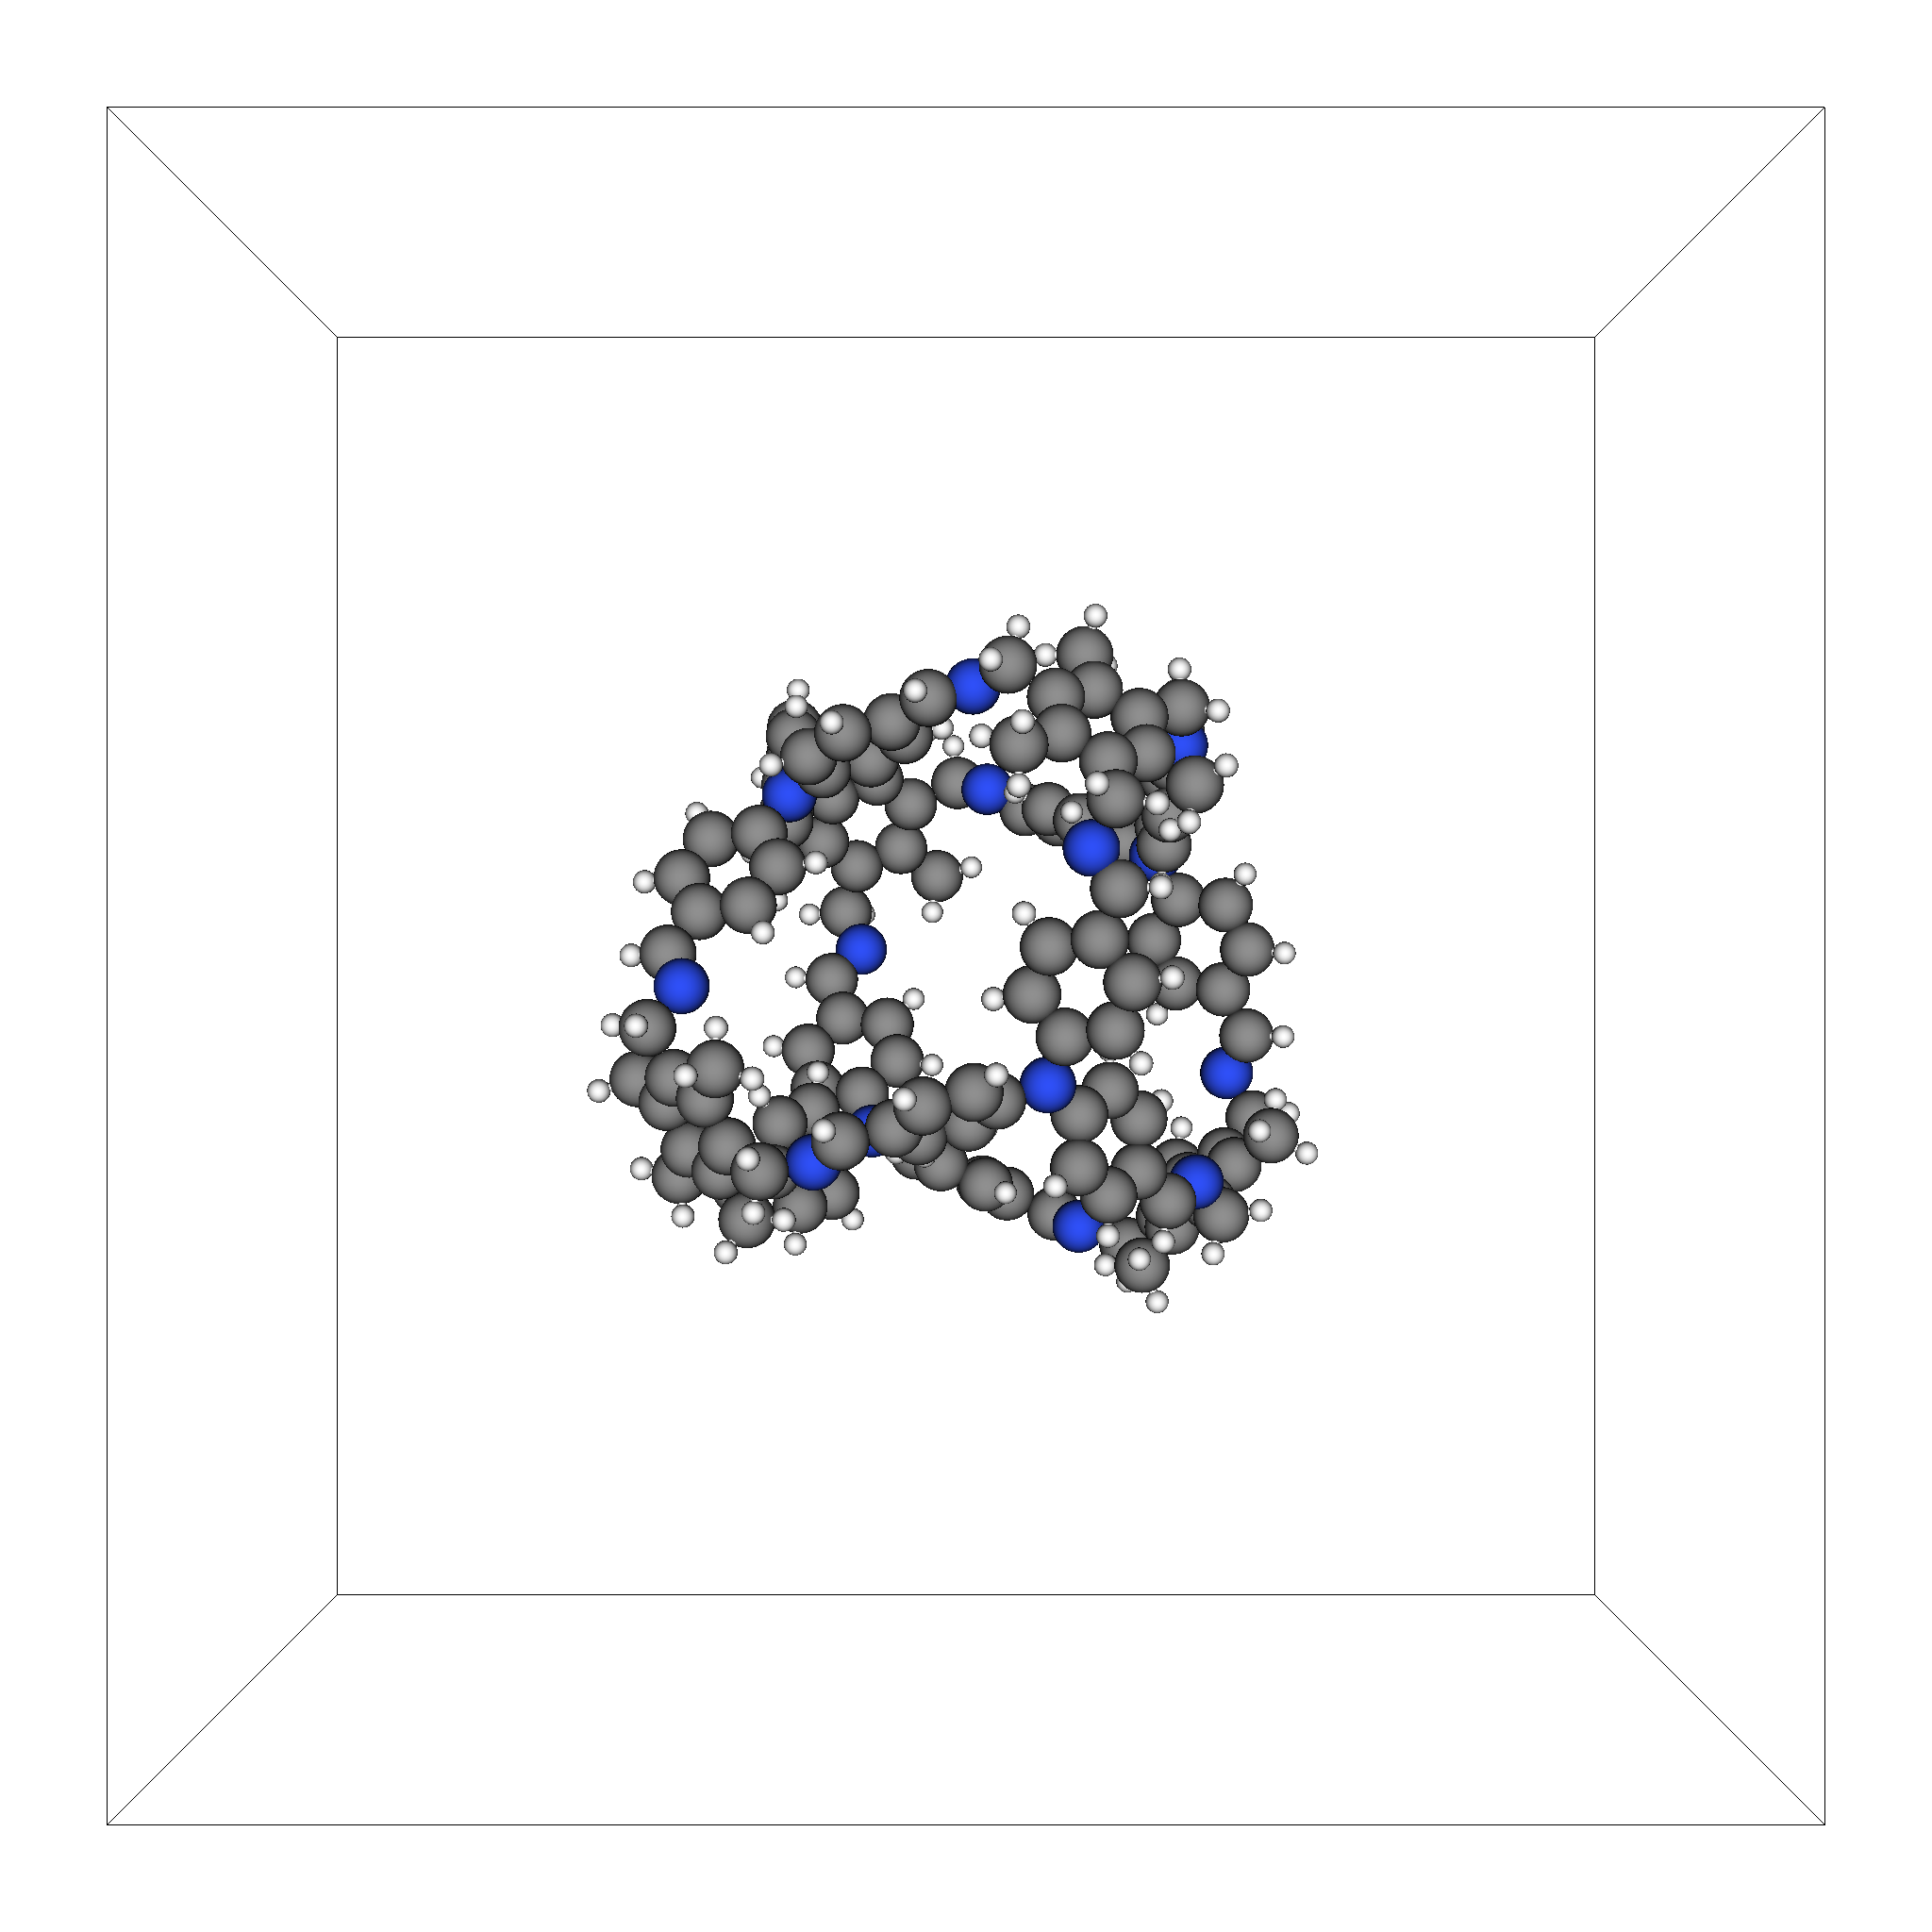
\includegraphics[width=0.25\columnwidth]{../final_aligned_cages/B23.png}}
\subfloat[B24]{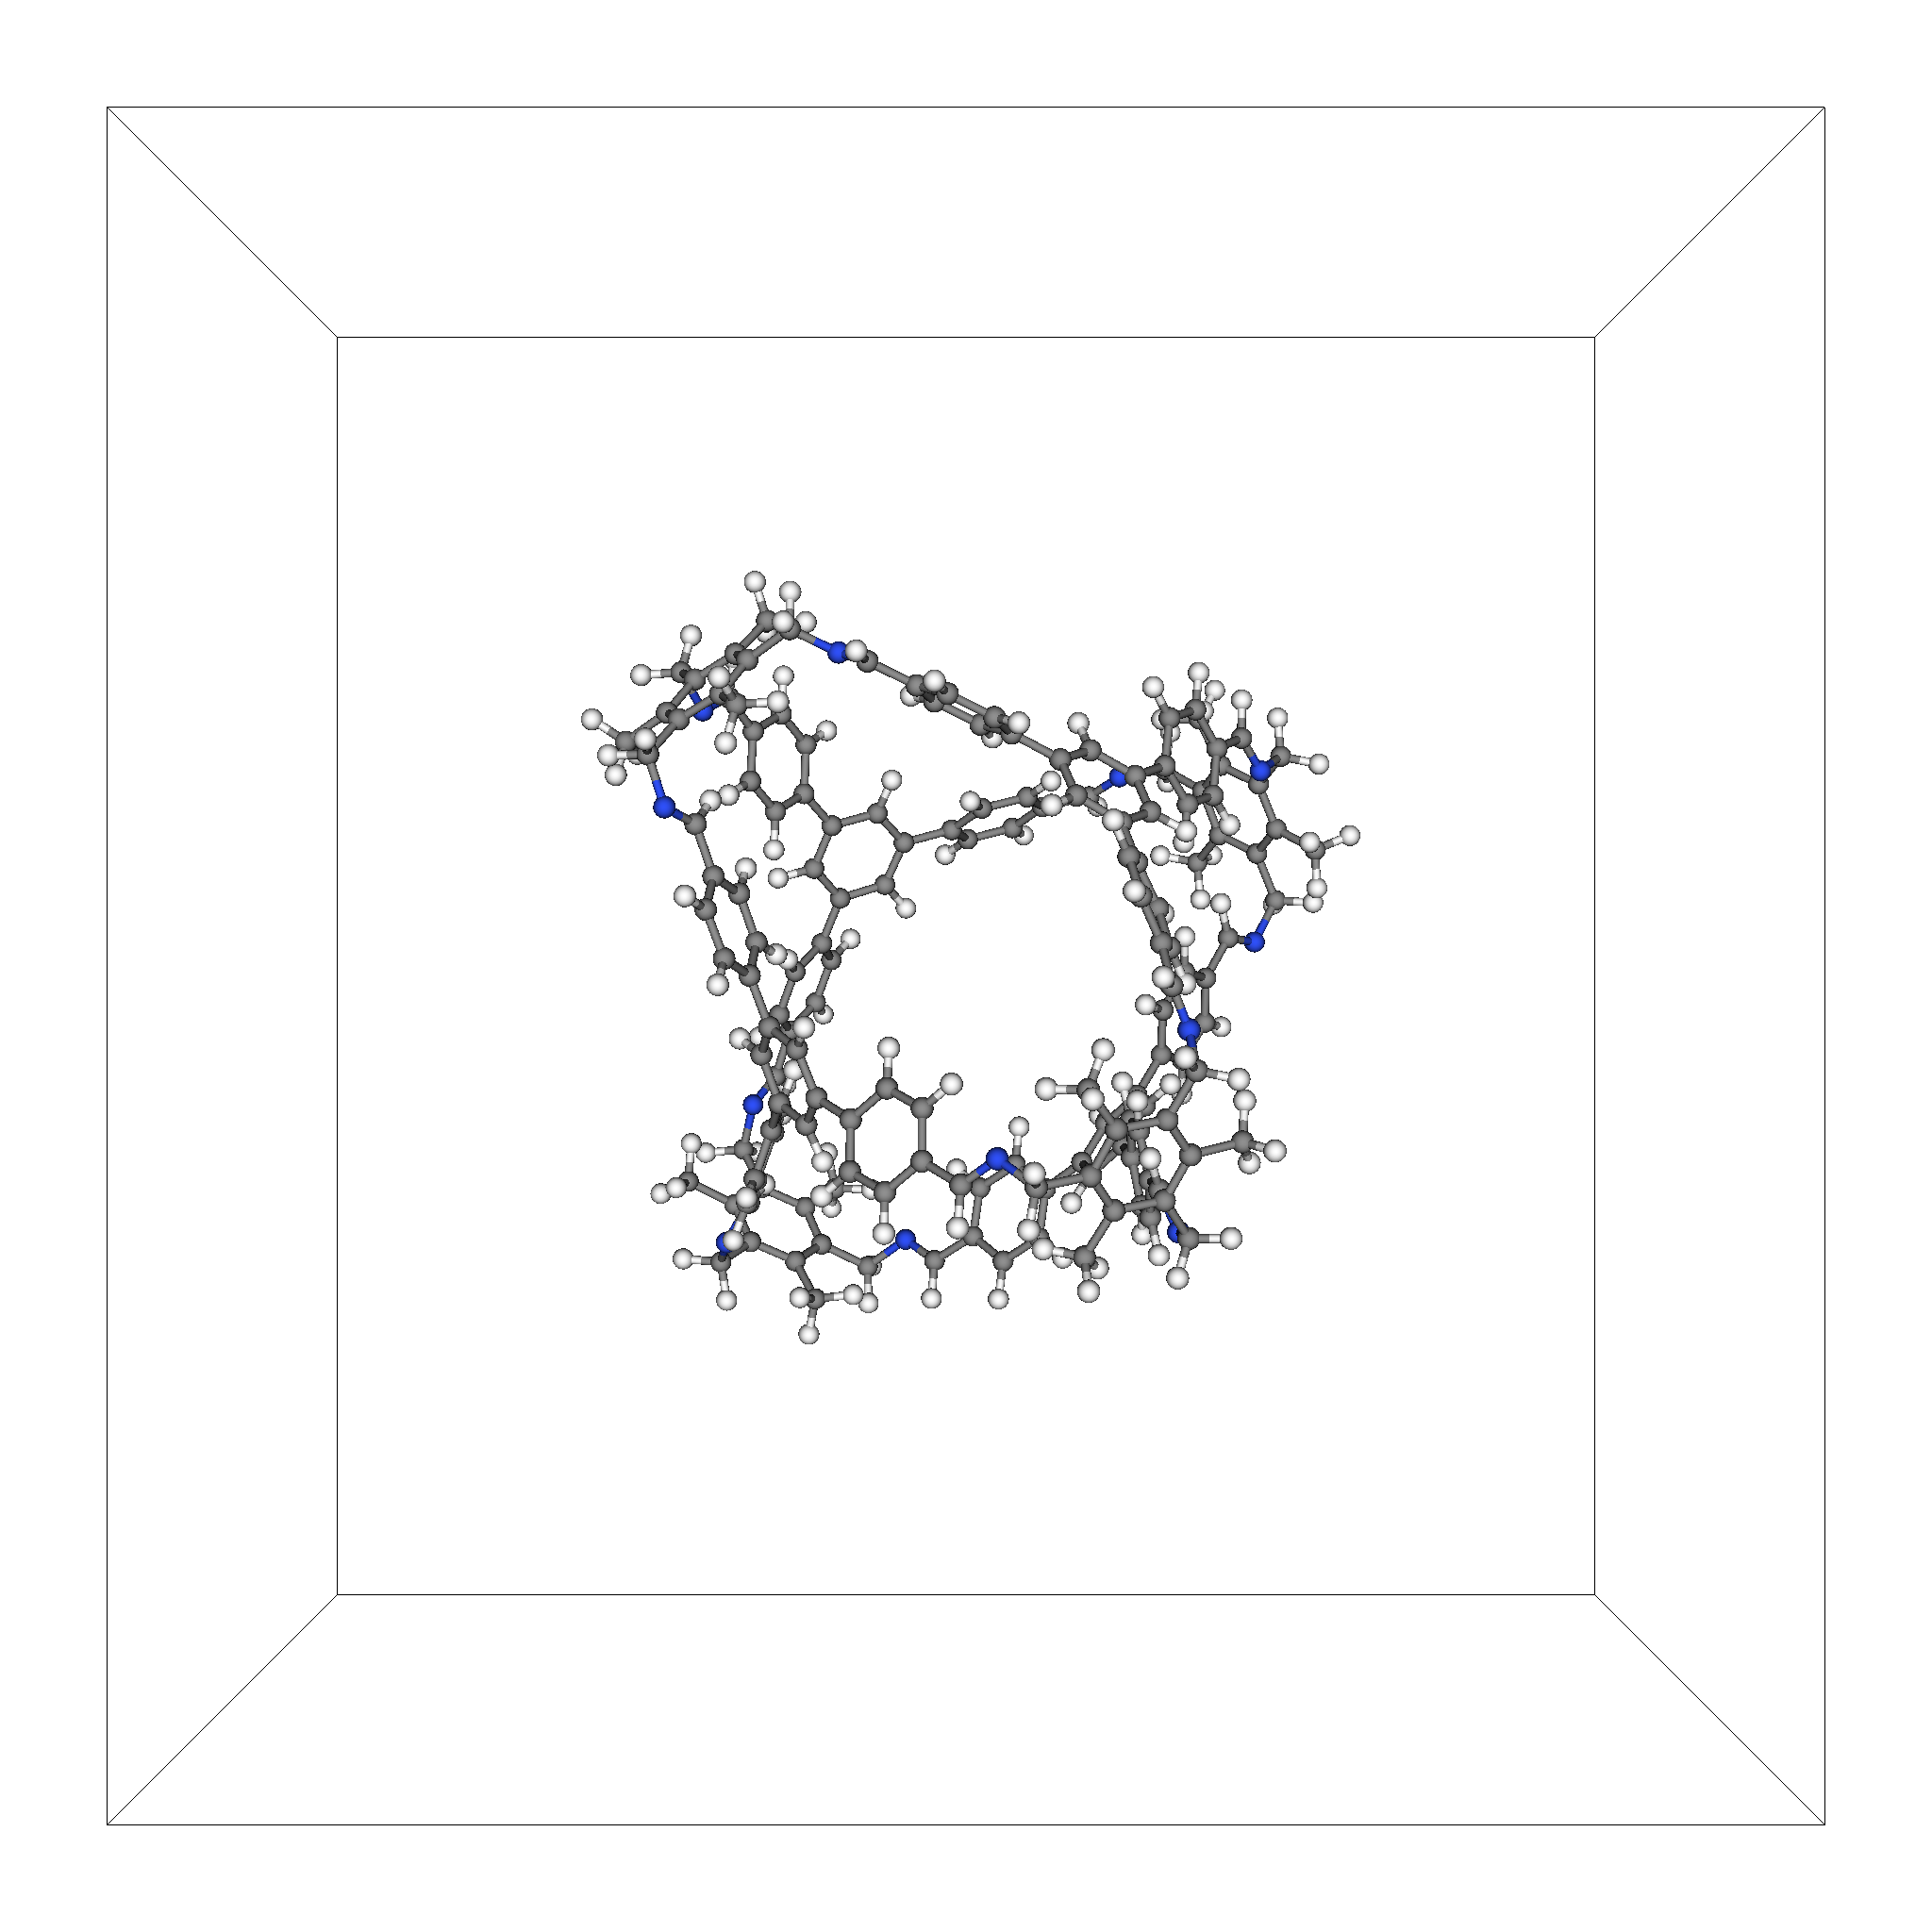
\includegraphics[width=0.25\columnwidth]{../final_aligned_cages/B24.png}}
\subfloat[B25]{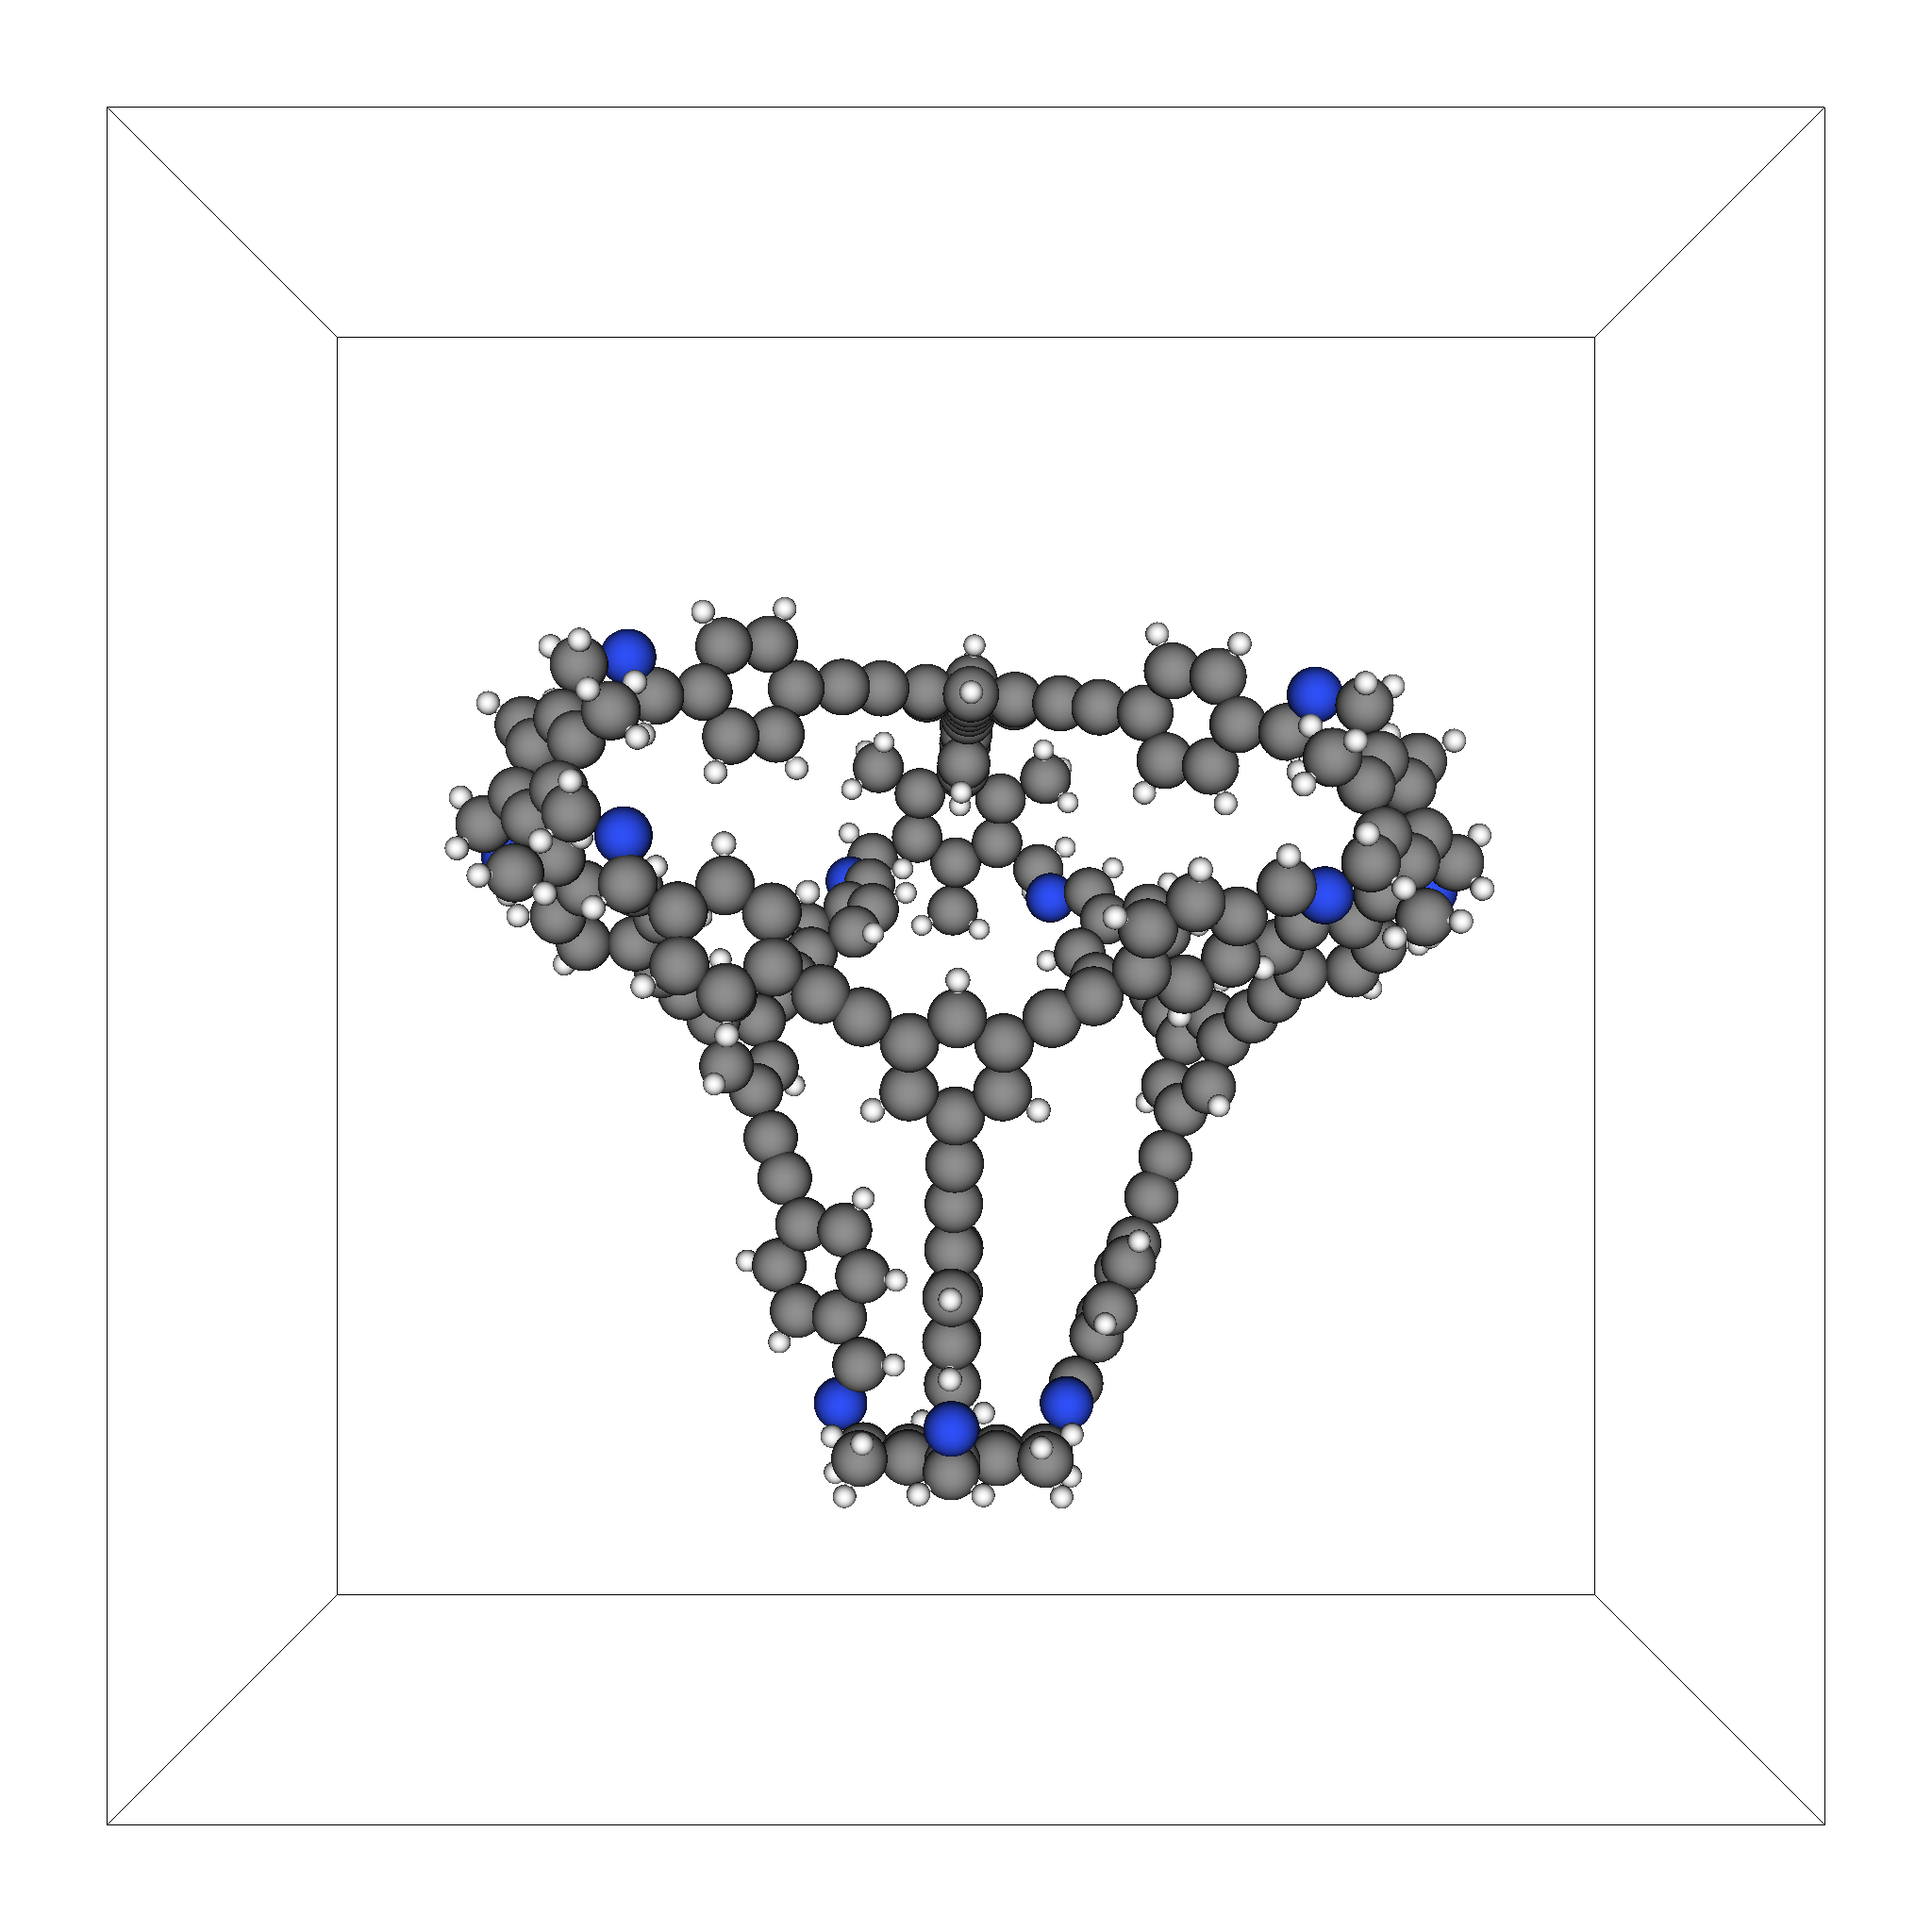
\includegraphics[width=0.25\columnwidth]{../final_aligned_cages/B25.png}}
\qquad
\subfloat[B26]{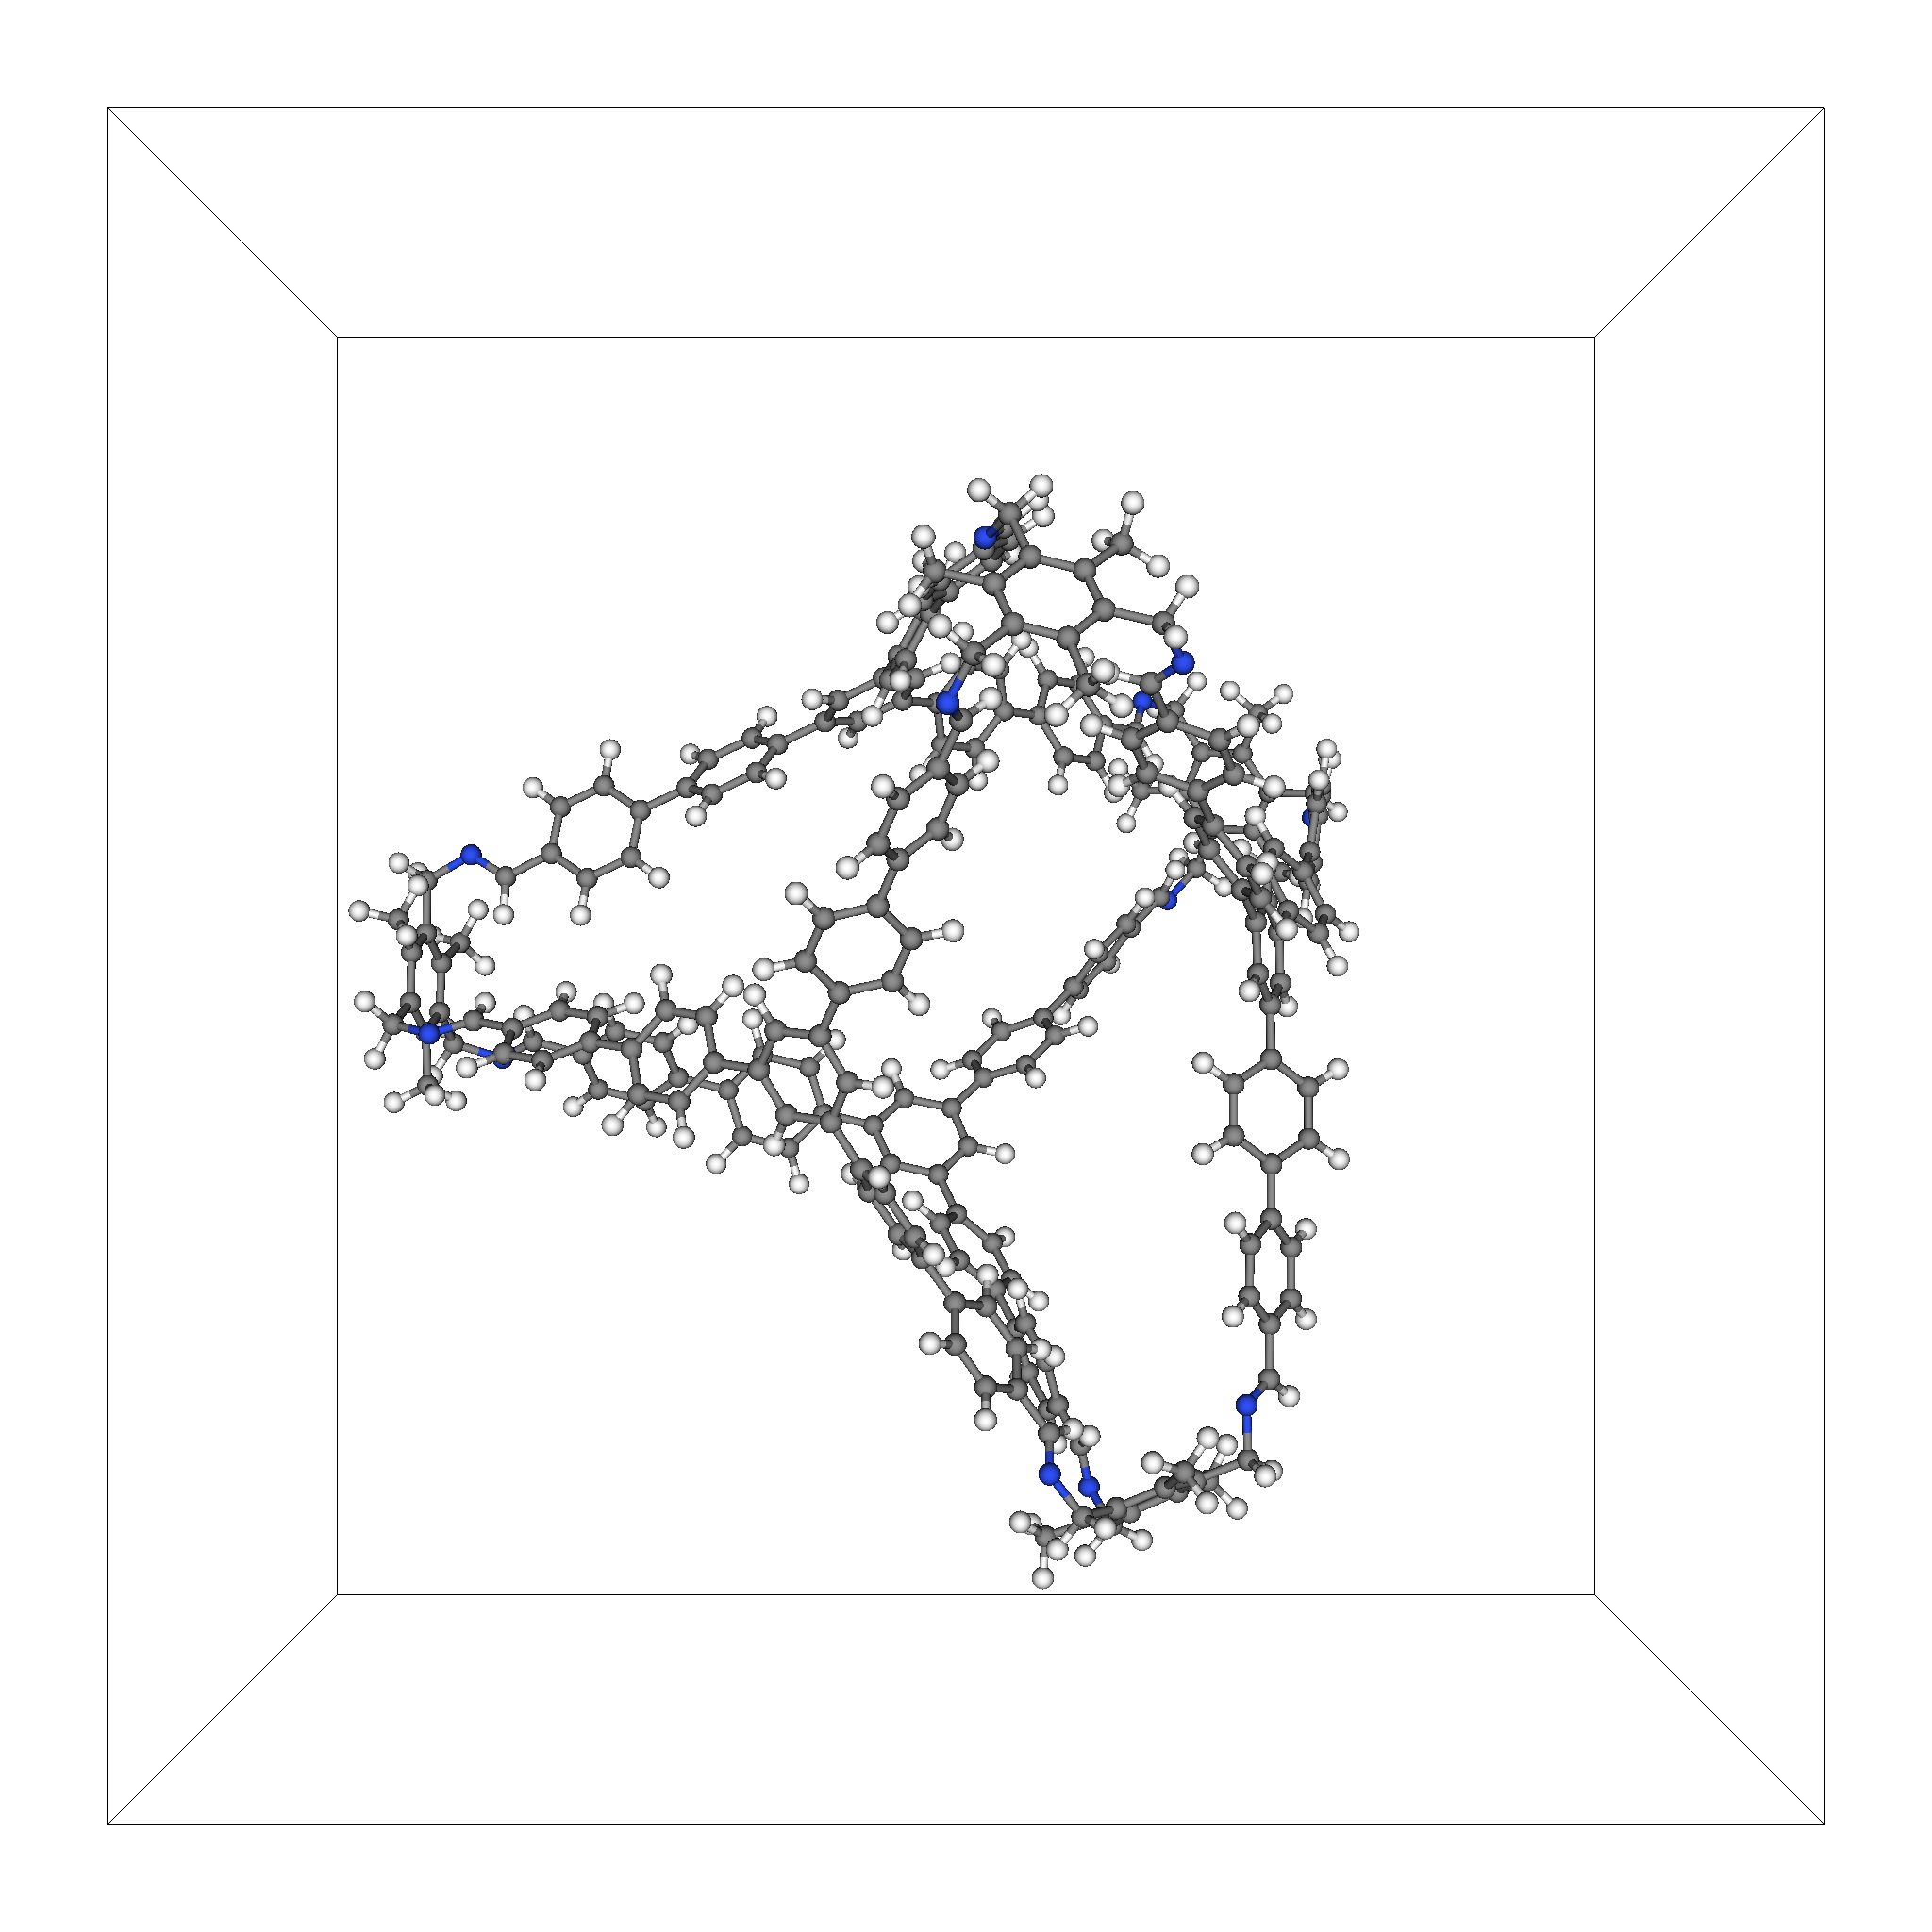
\includegraphics[width=0.25\columnwidth]{../final_aligned_cages/B26.png}}
\subfloat[B2]{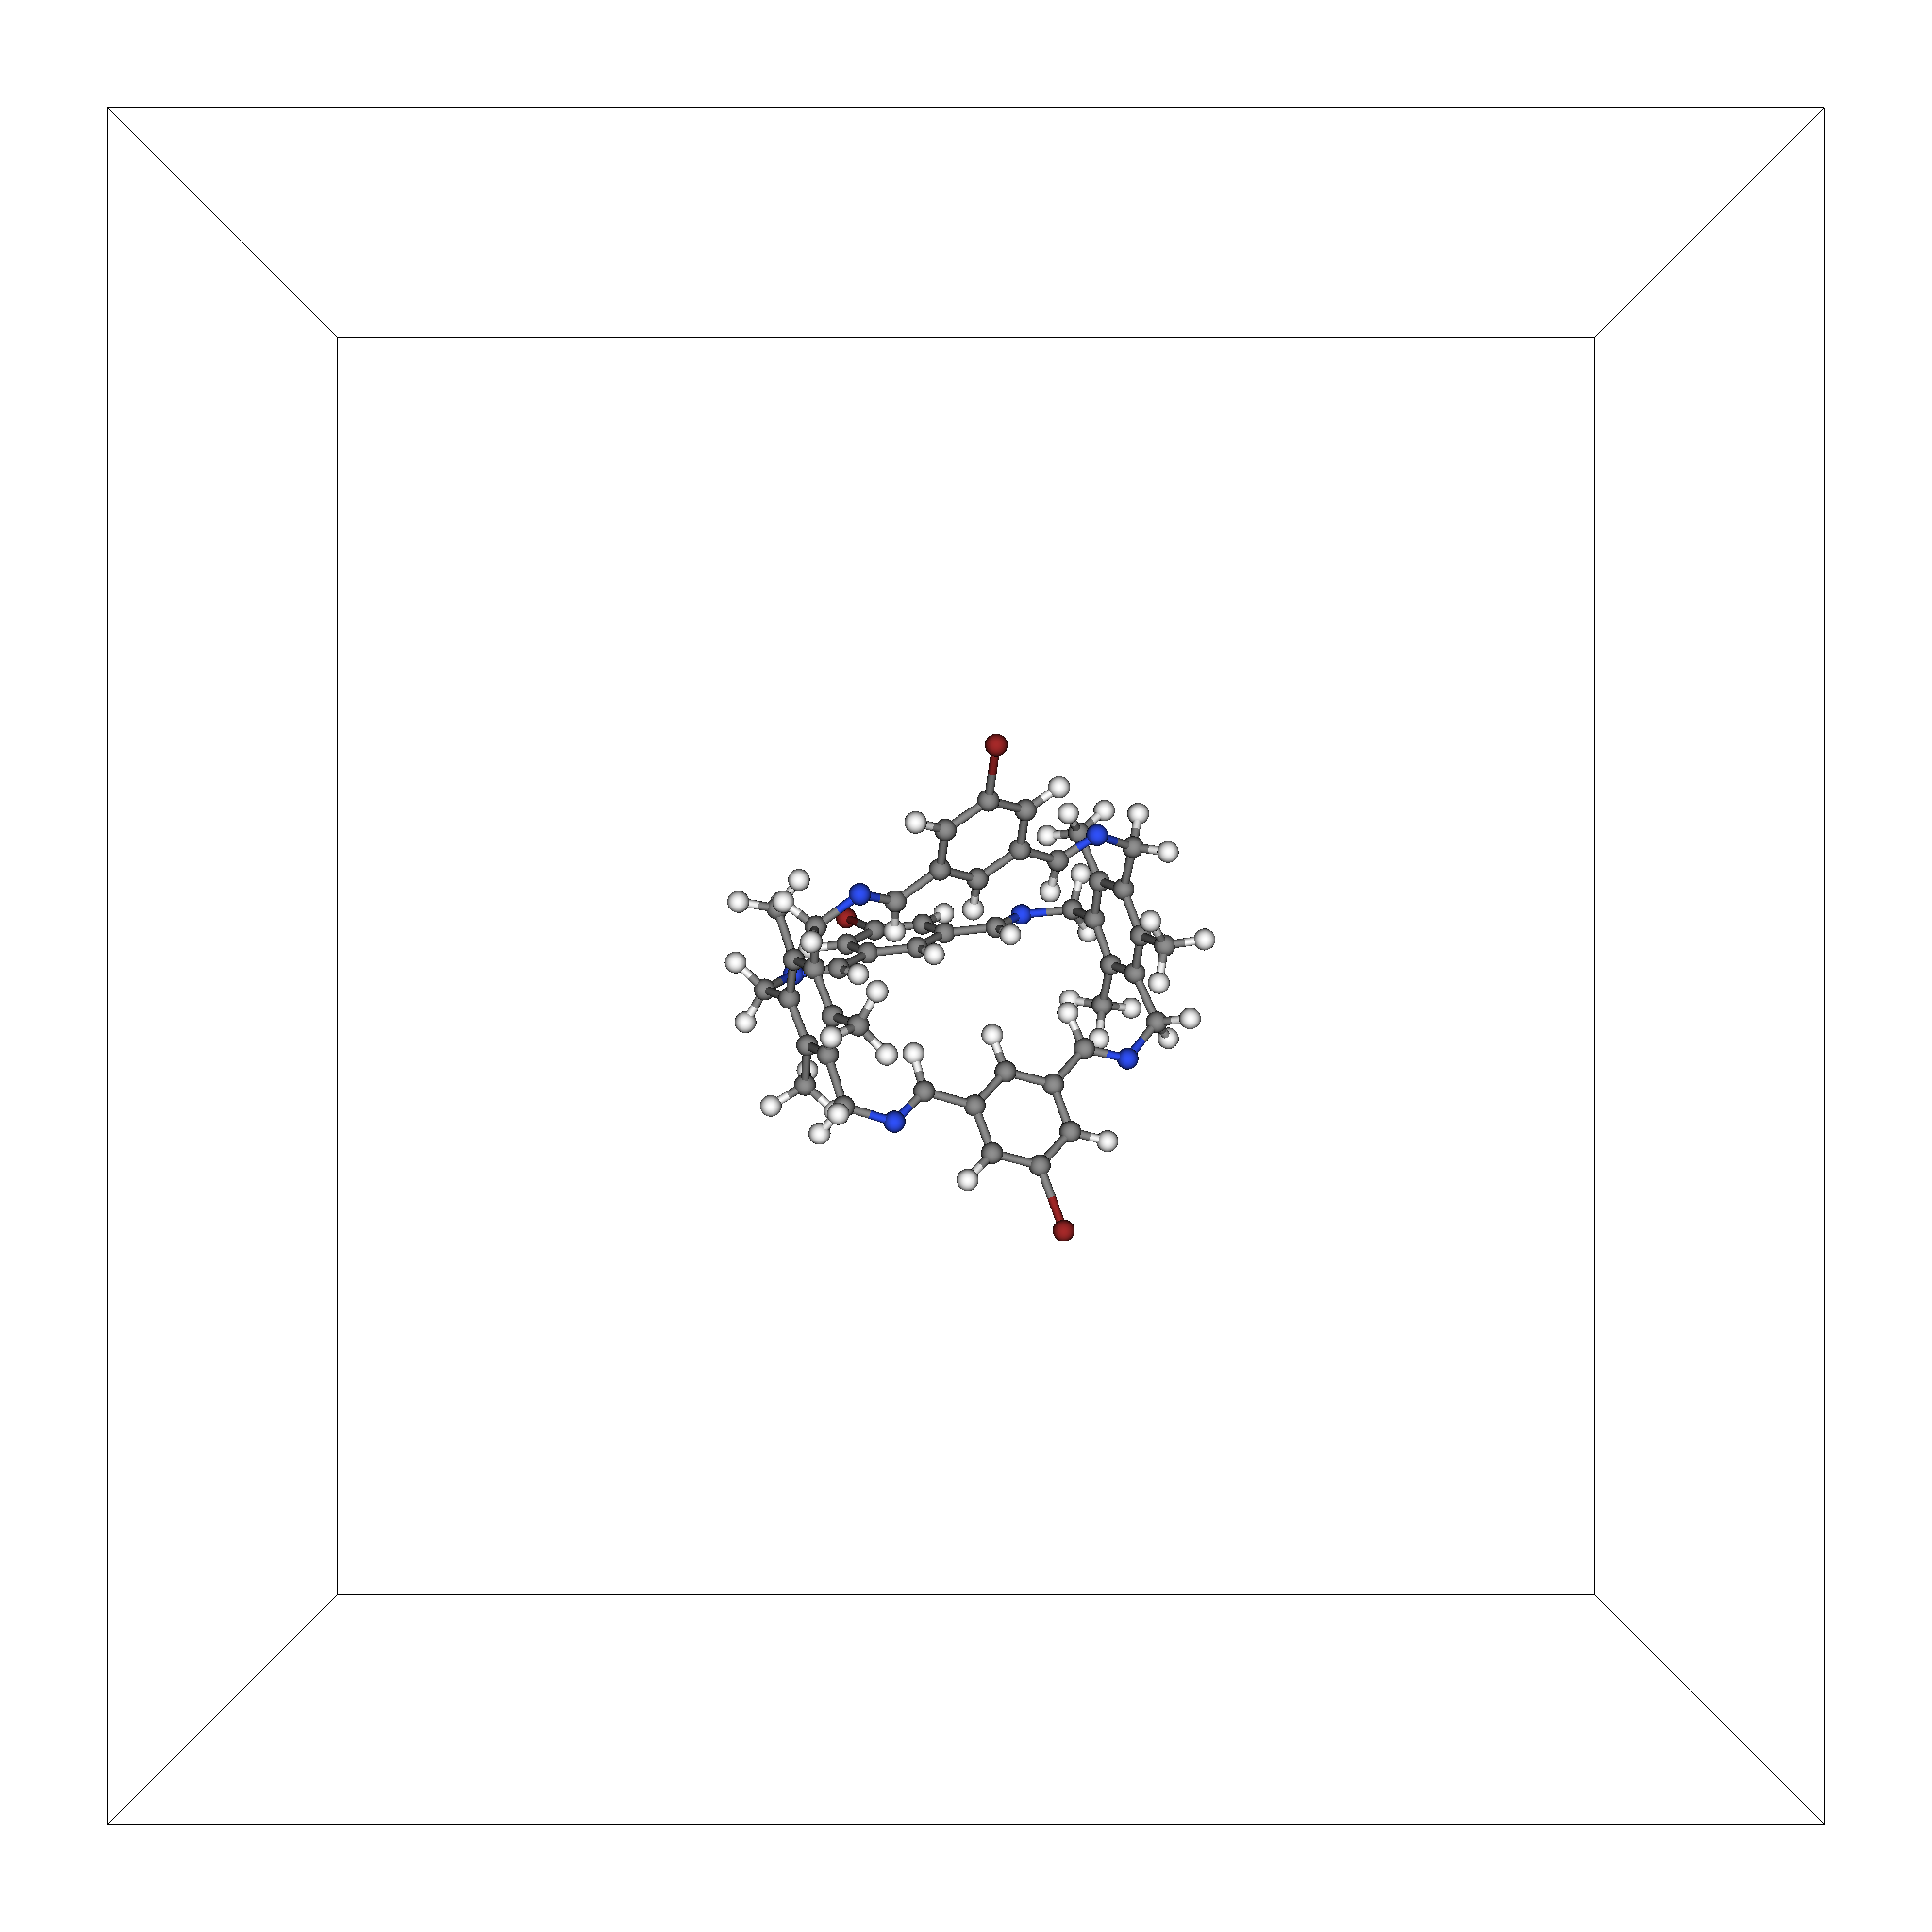
\includegraphics[width=0.25\columnwidth]{../final_aligned_cages/B2.png}}
\subfloat[B4]{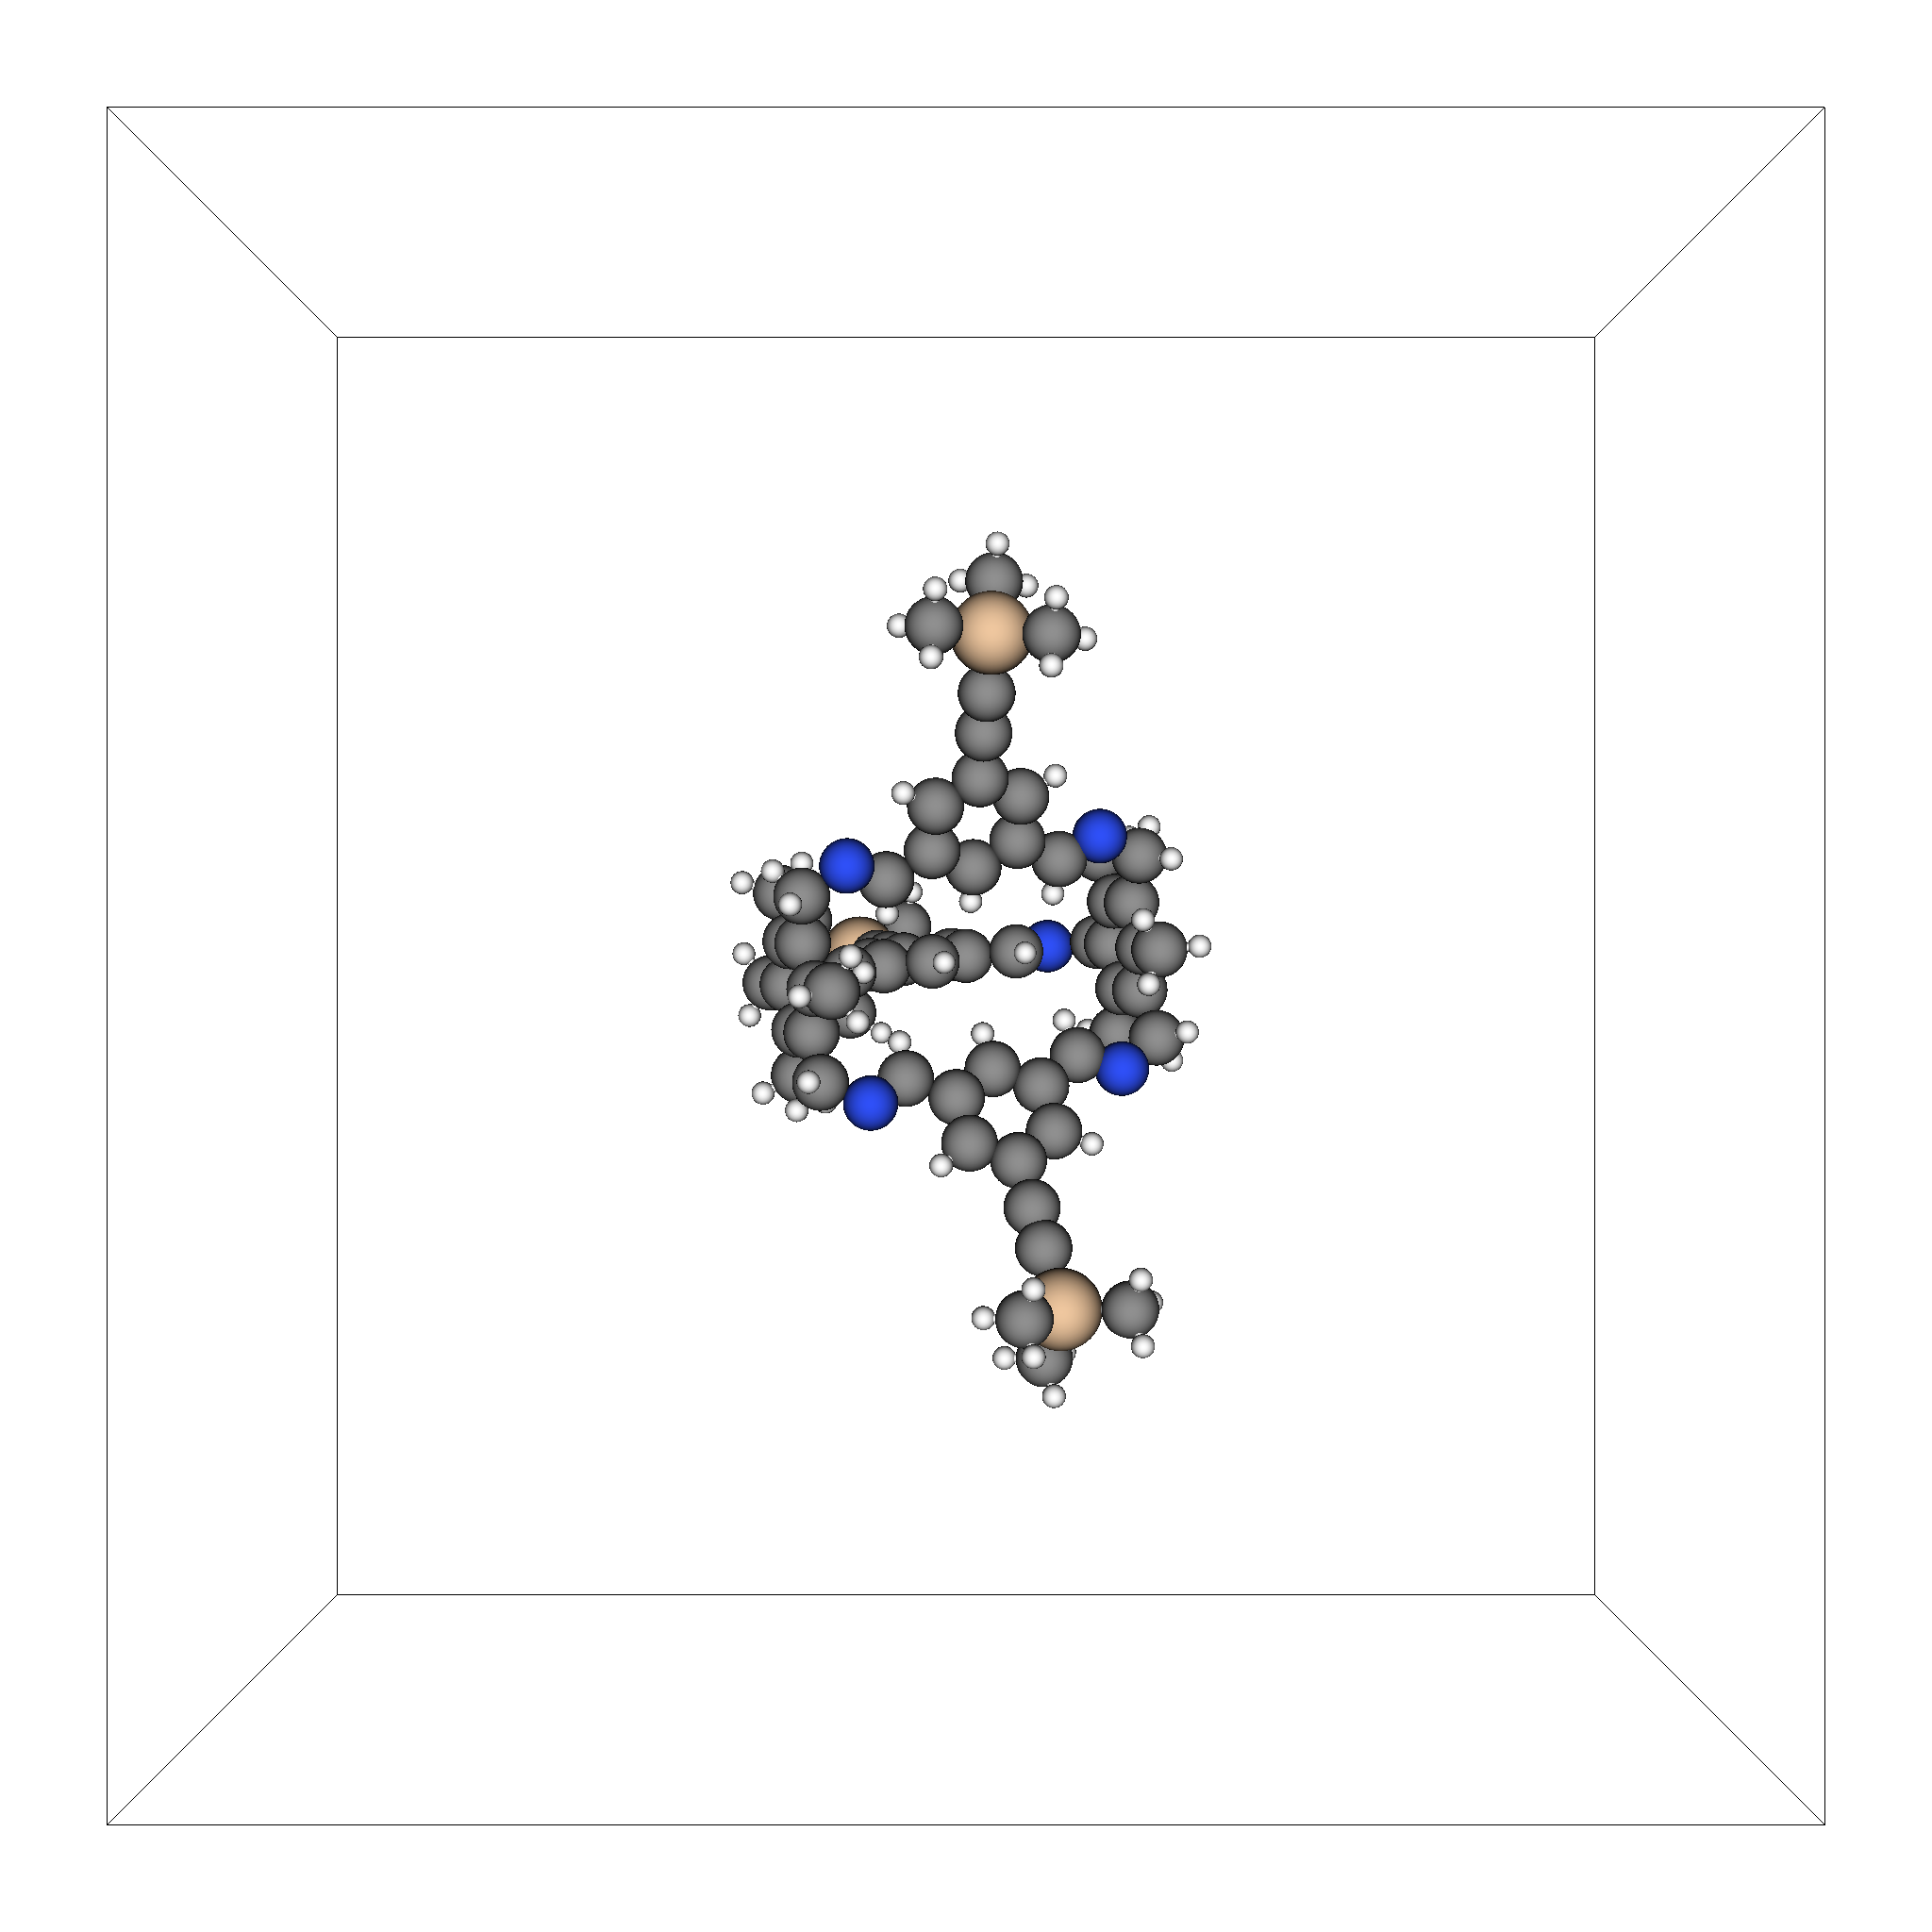
\includegraphics[width=0.25\columnwidth]{../final_aligned_cages/B4.png}}
\phantomcaption \end{figure}
\begin{figure}
\ContinuedFloat \centering
\subfloat[B5]{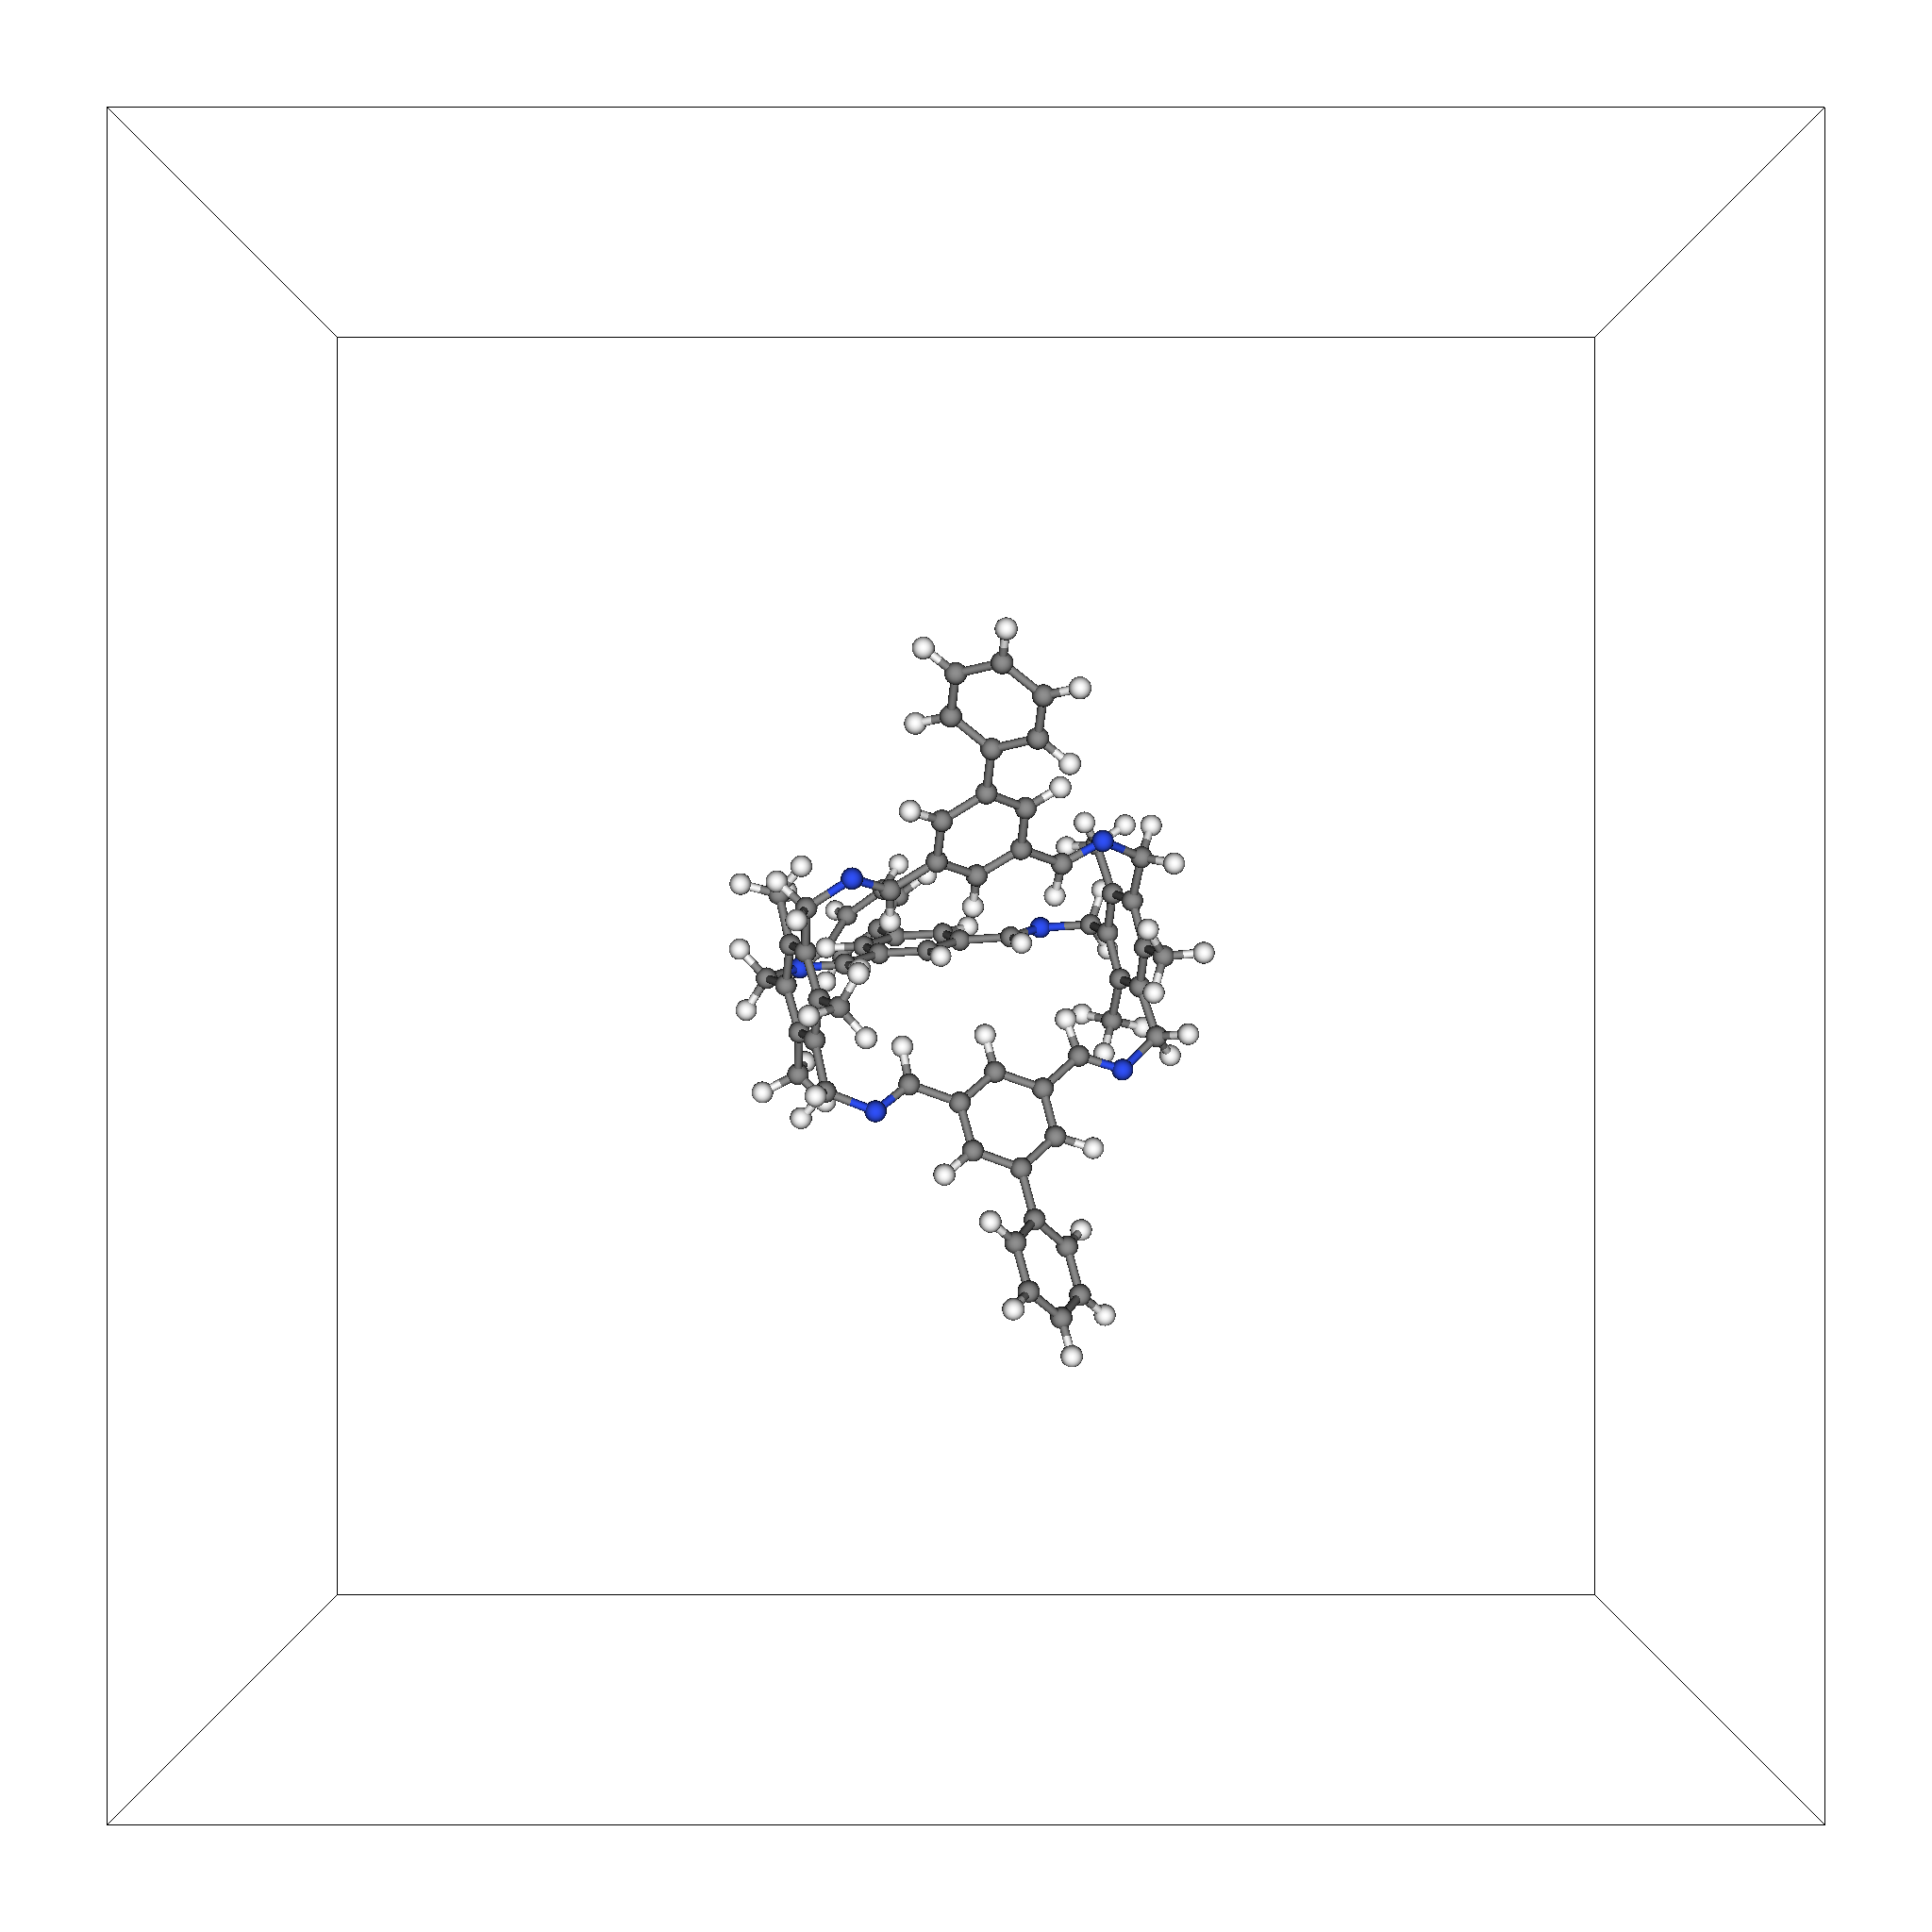
\includegraphics[width=0.25\columnwidth]{../final_aligned_cages/B5.png}}
\subfloat[B6]{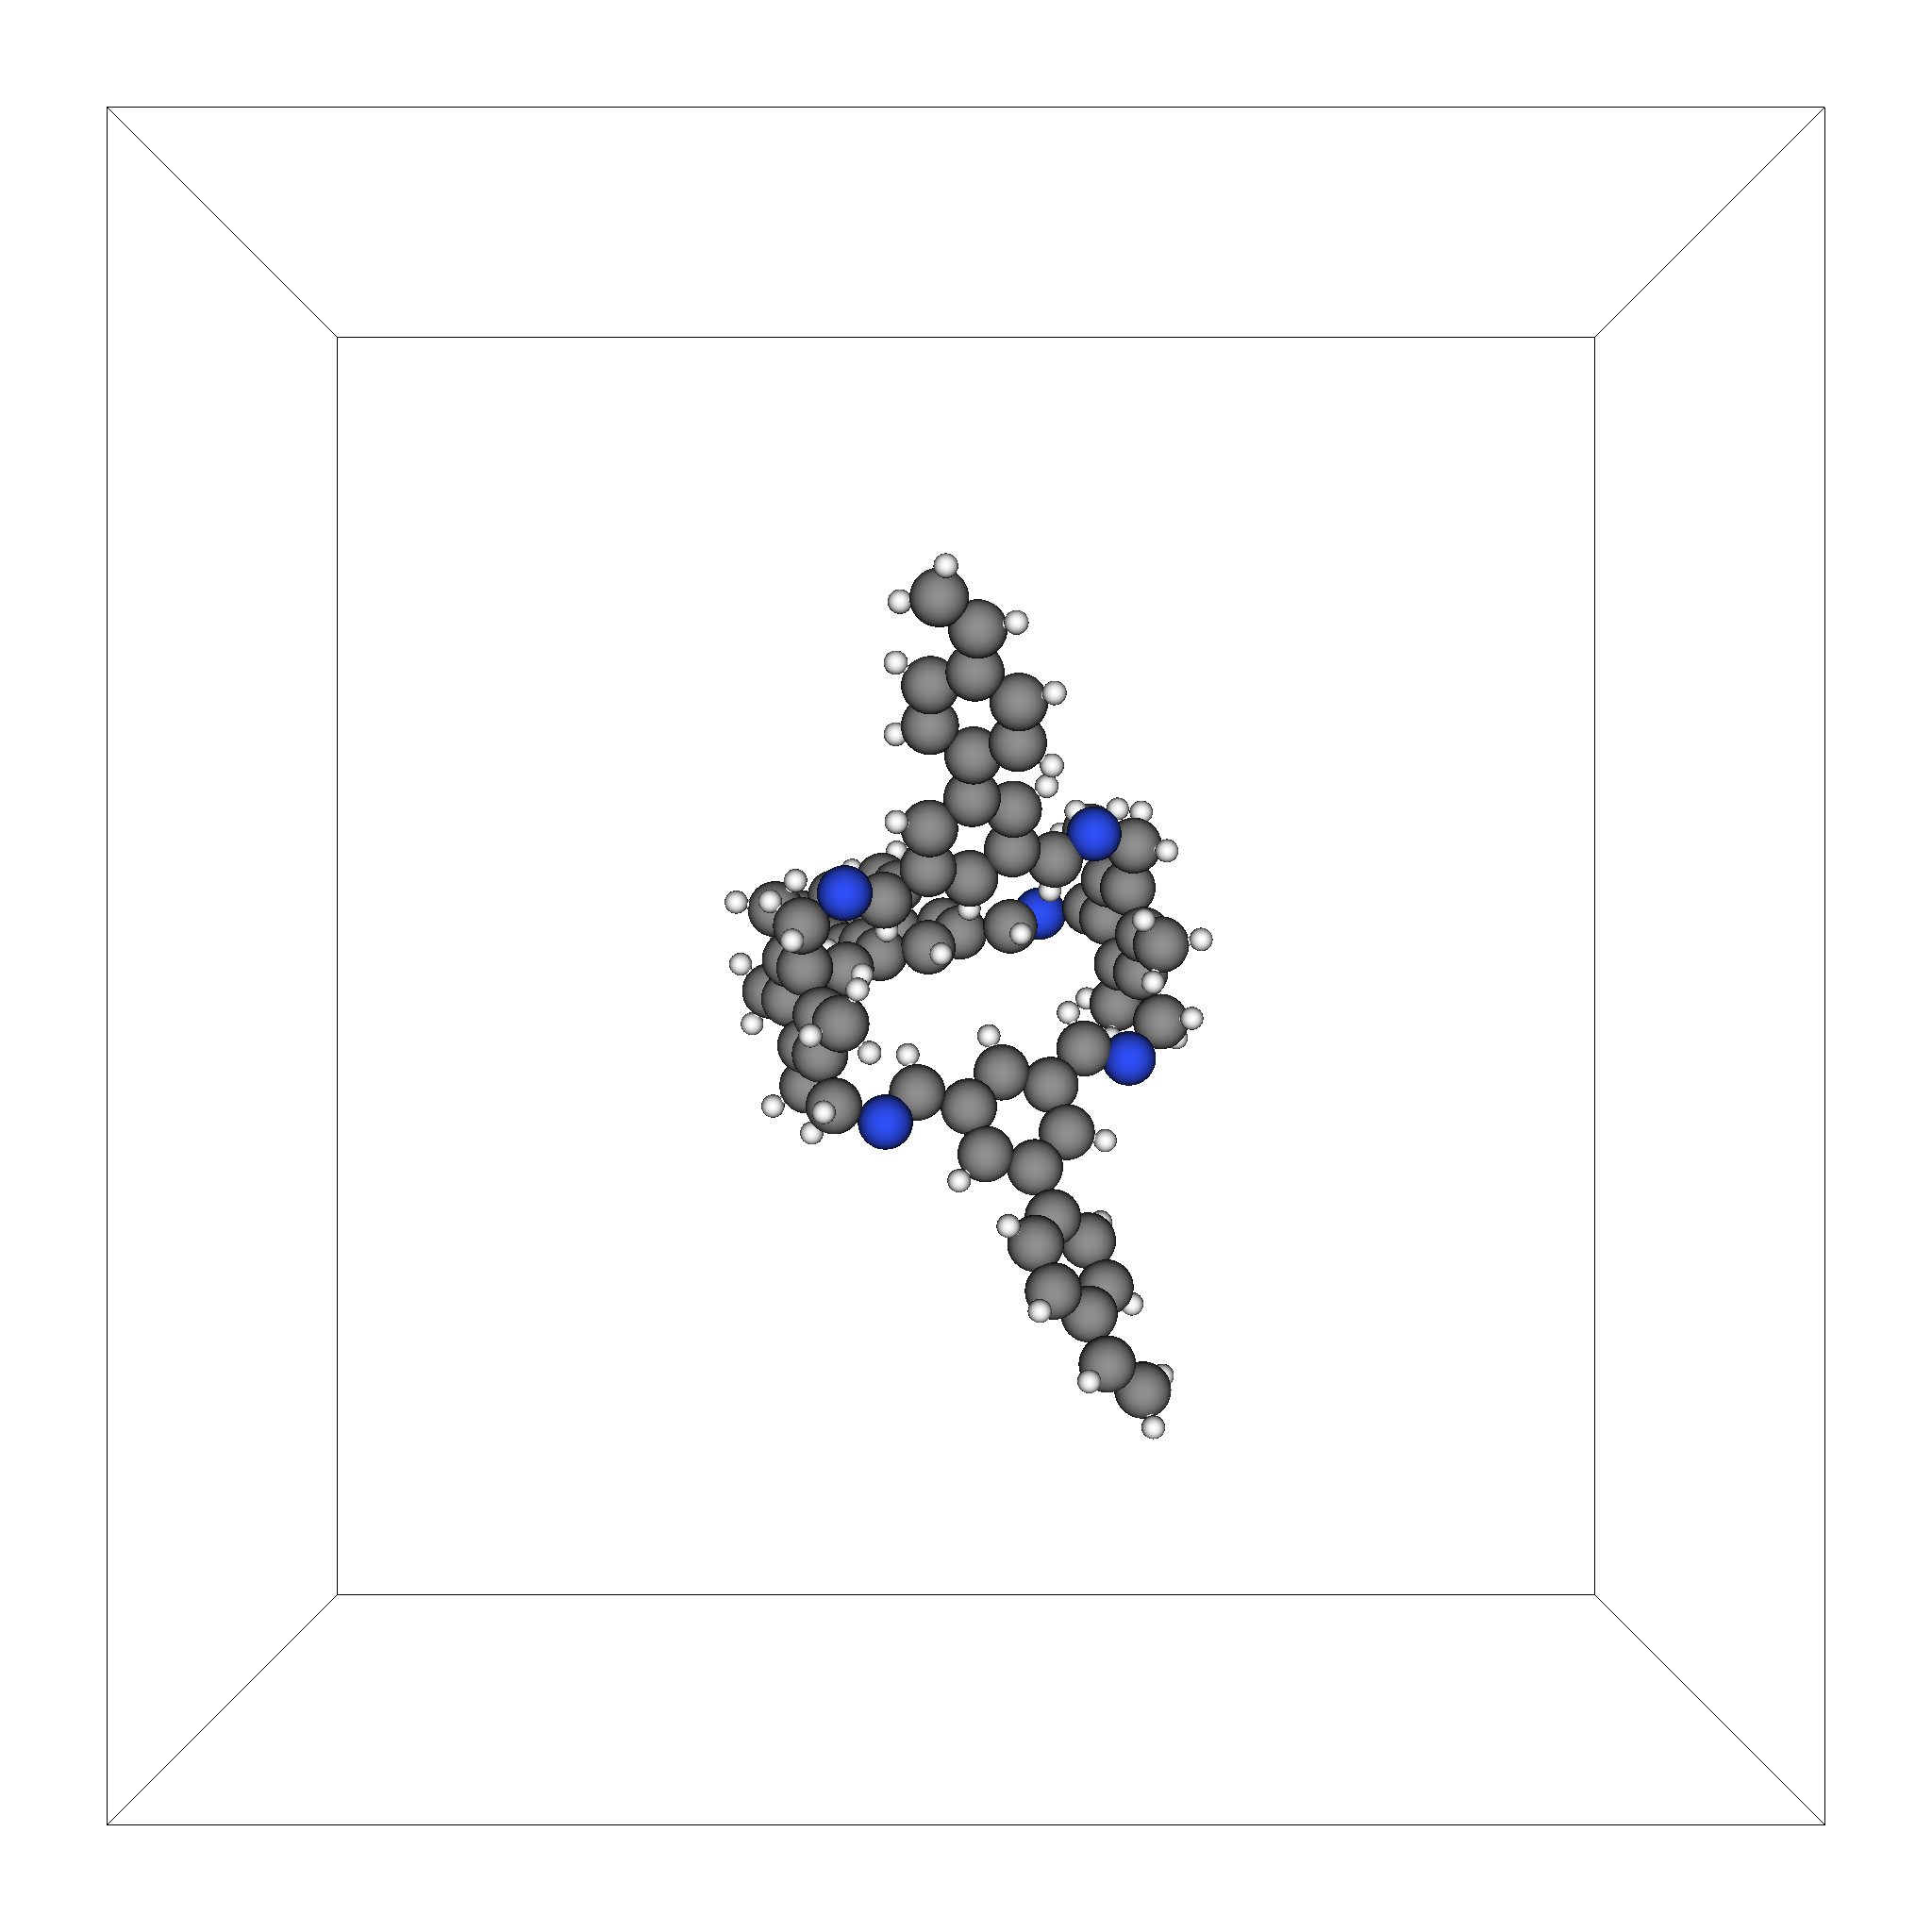
\includegraphics[width=0.25\columnwidth]{../final_aligned_cages/B6.png}}
\subfloat[B8]{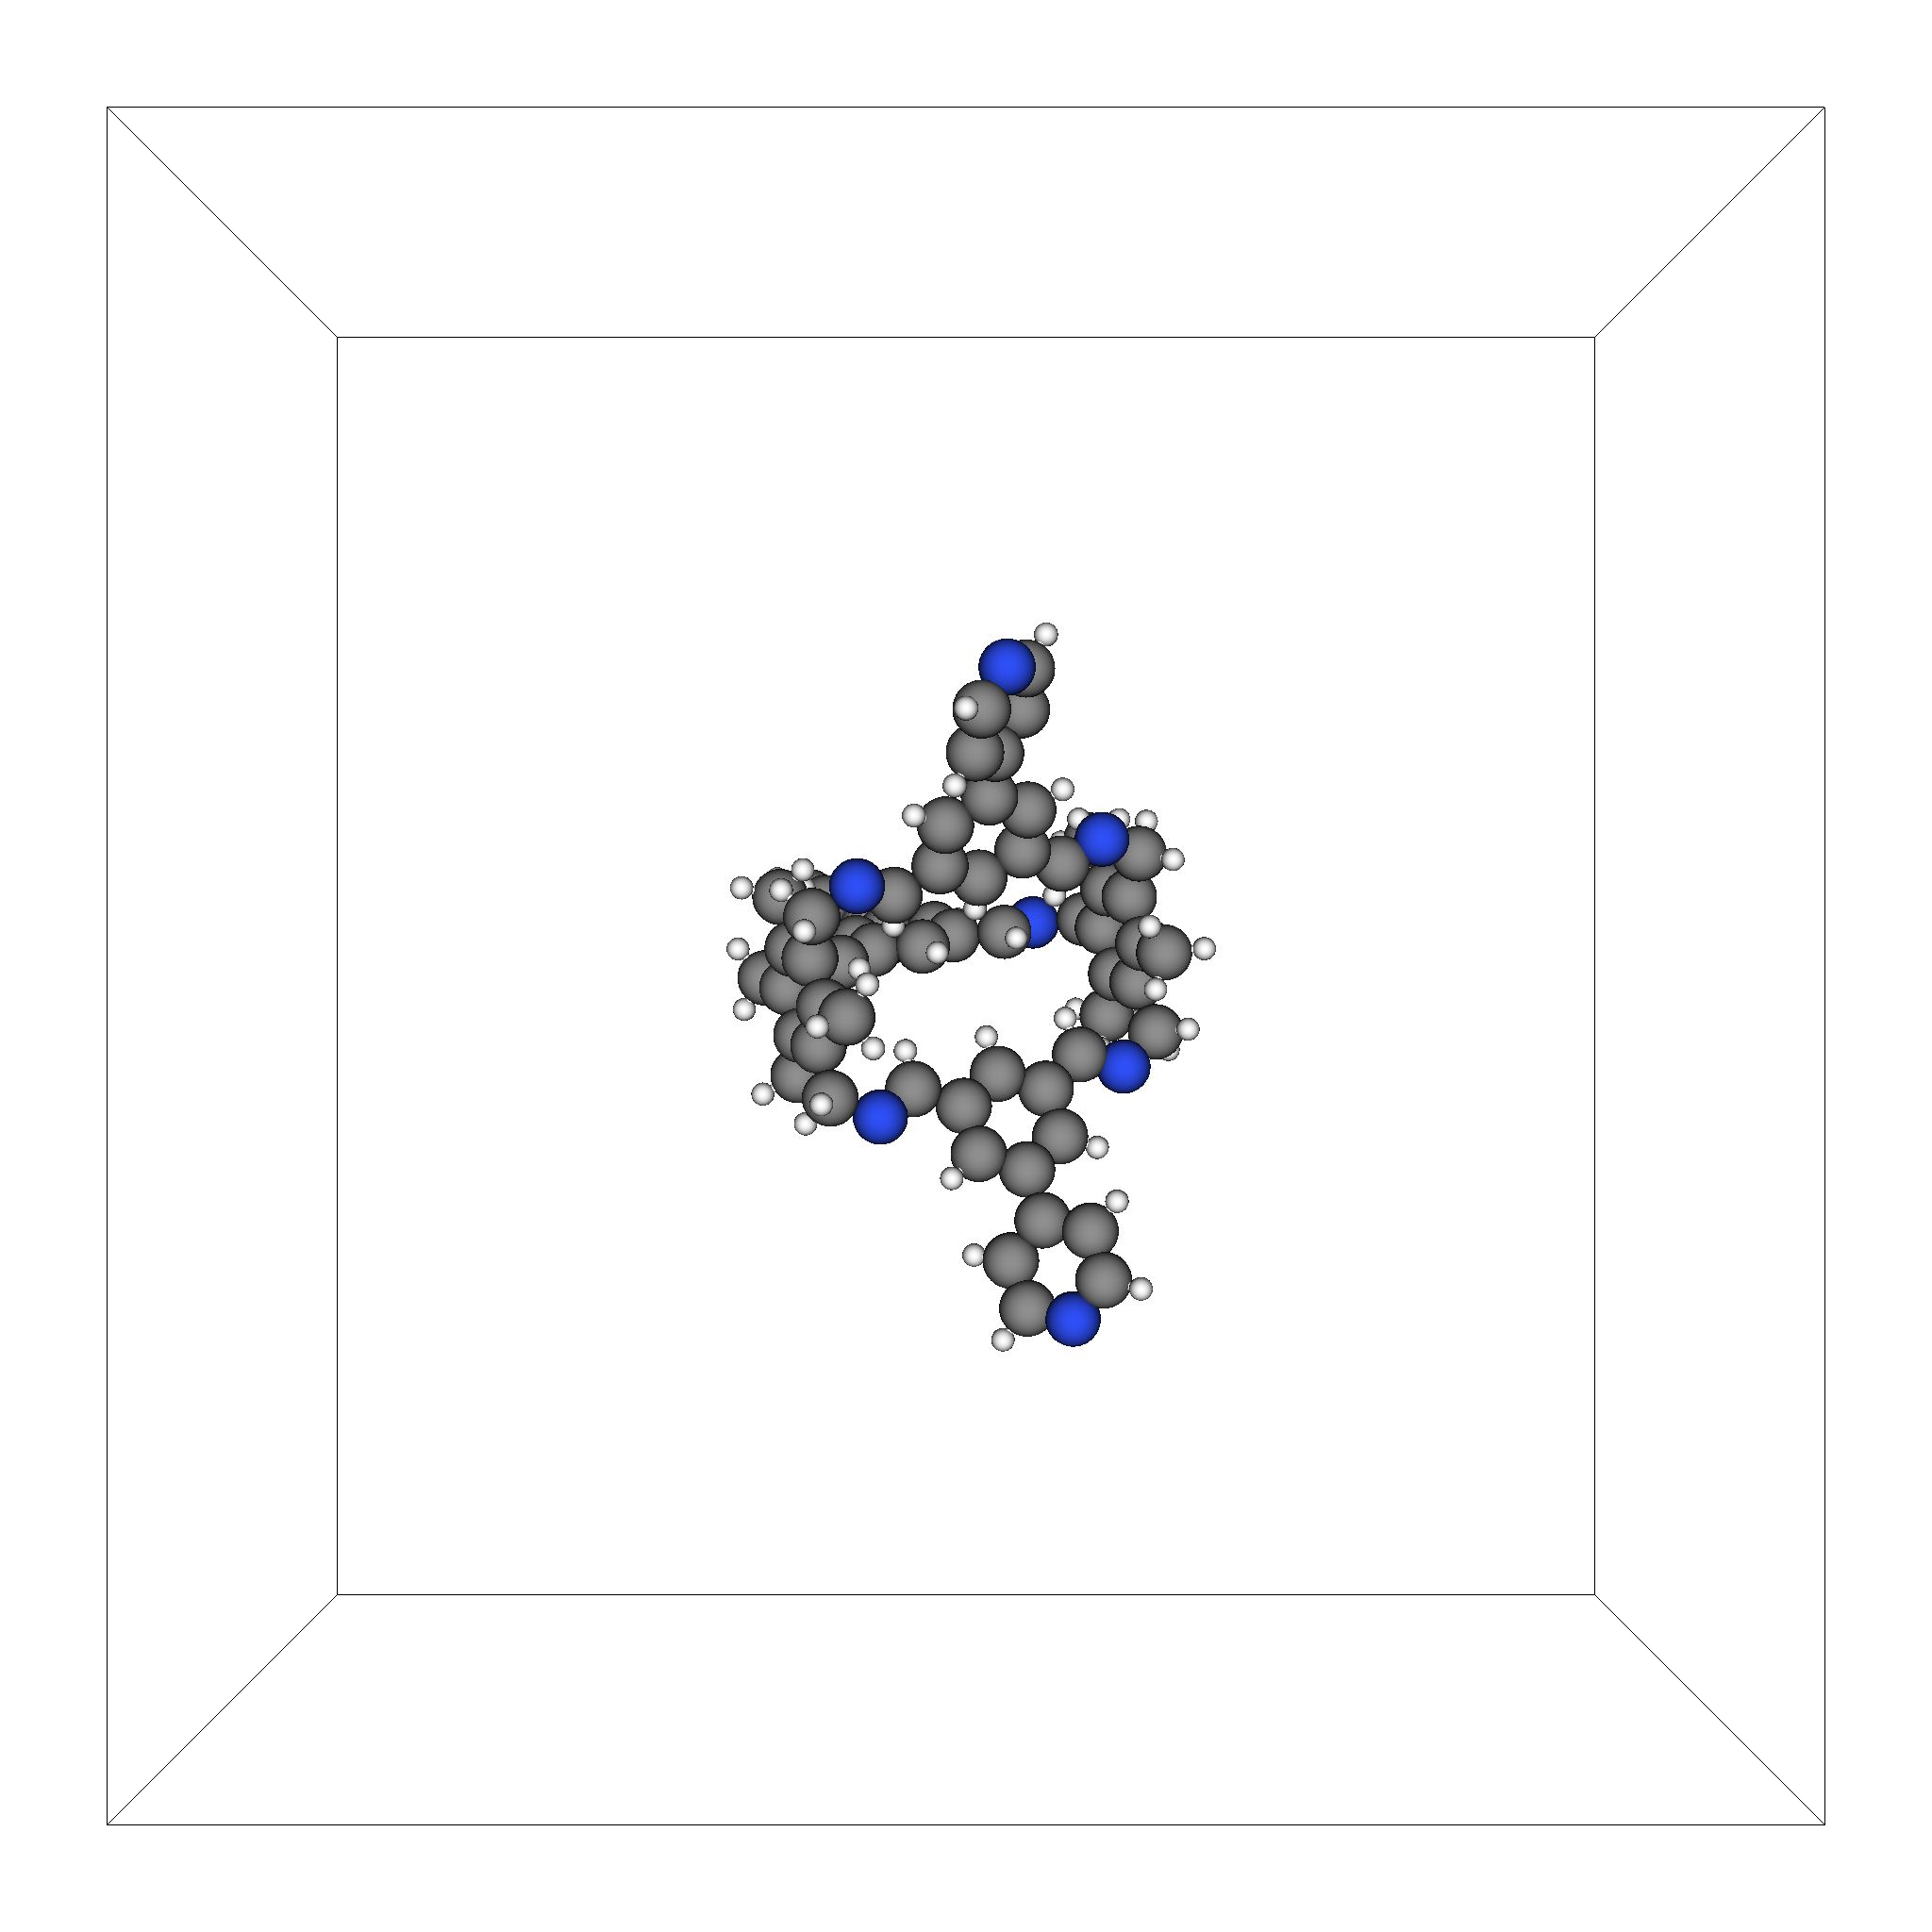
\includegraphics[width=0.25\columnwidth]{../final_aligned_cages/B8.png}}
\qquad
\subfloat[B9]{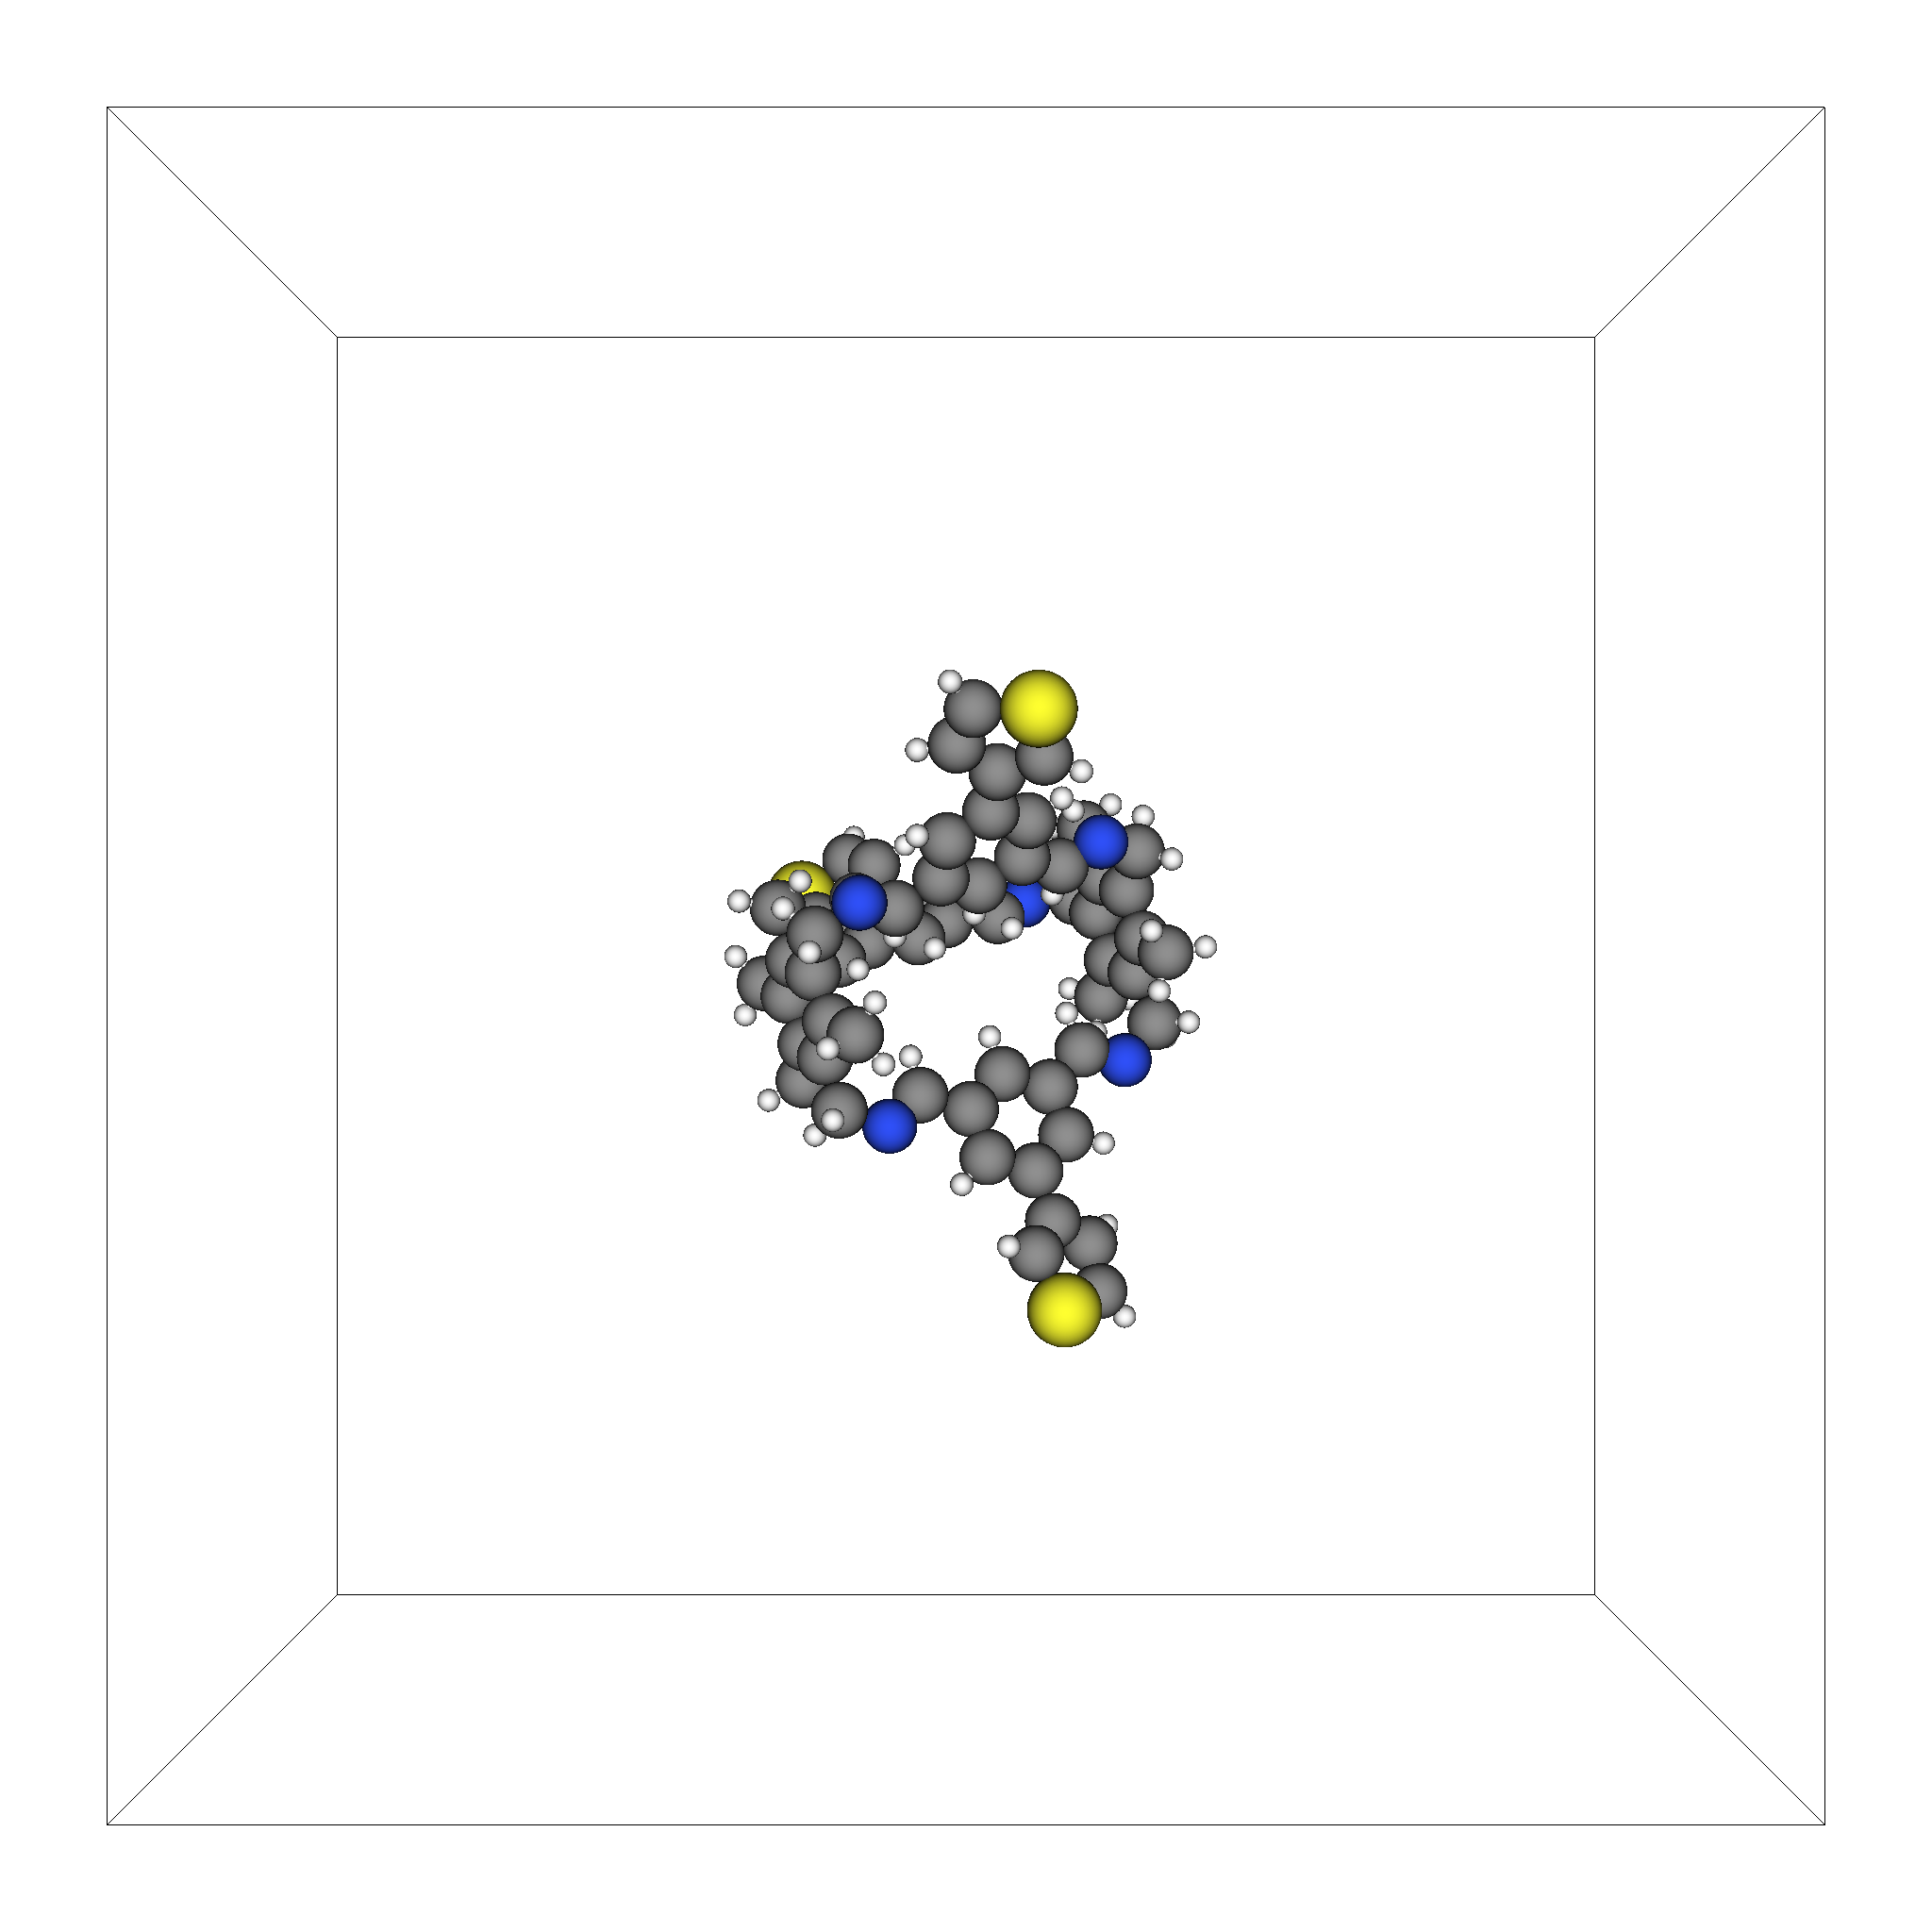
\includegraphics[width=0.25\columnwidth]{../final_aligned_cages/B9.png}}
\subfloat[C11]{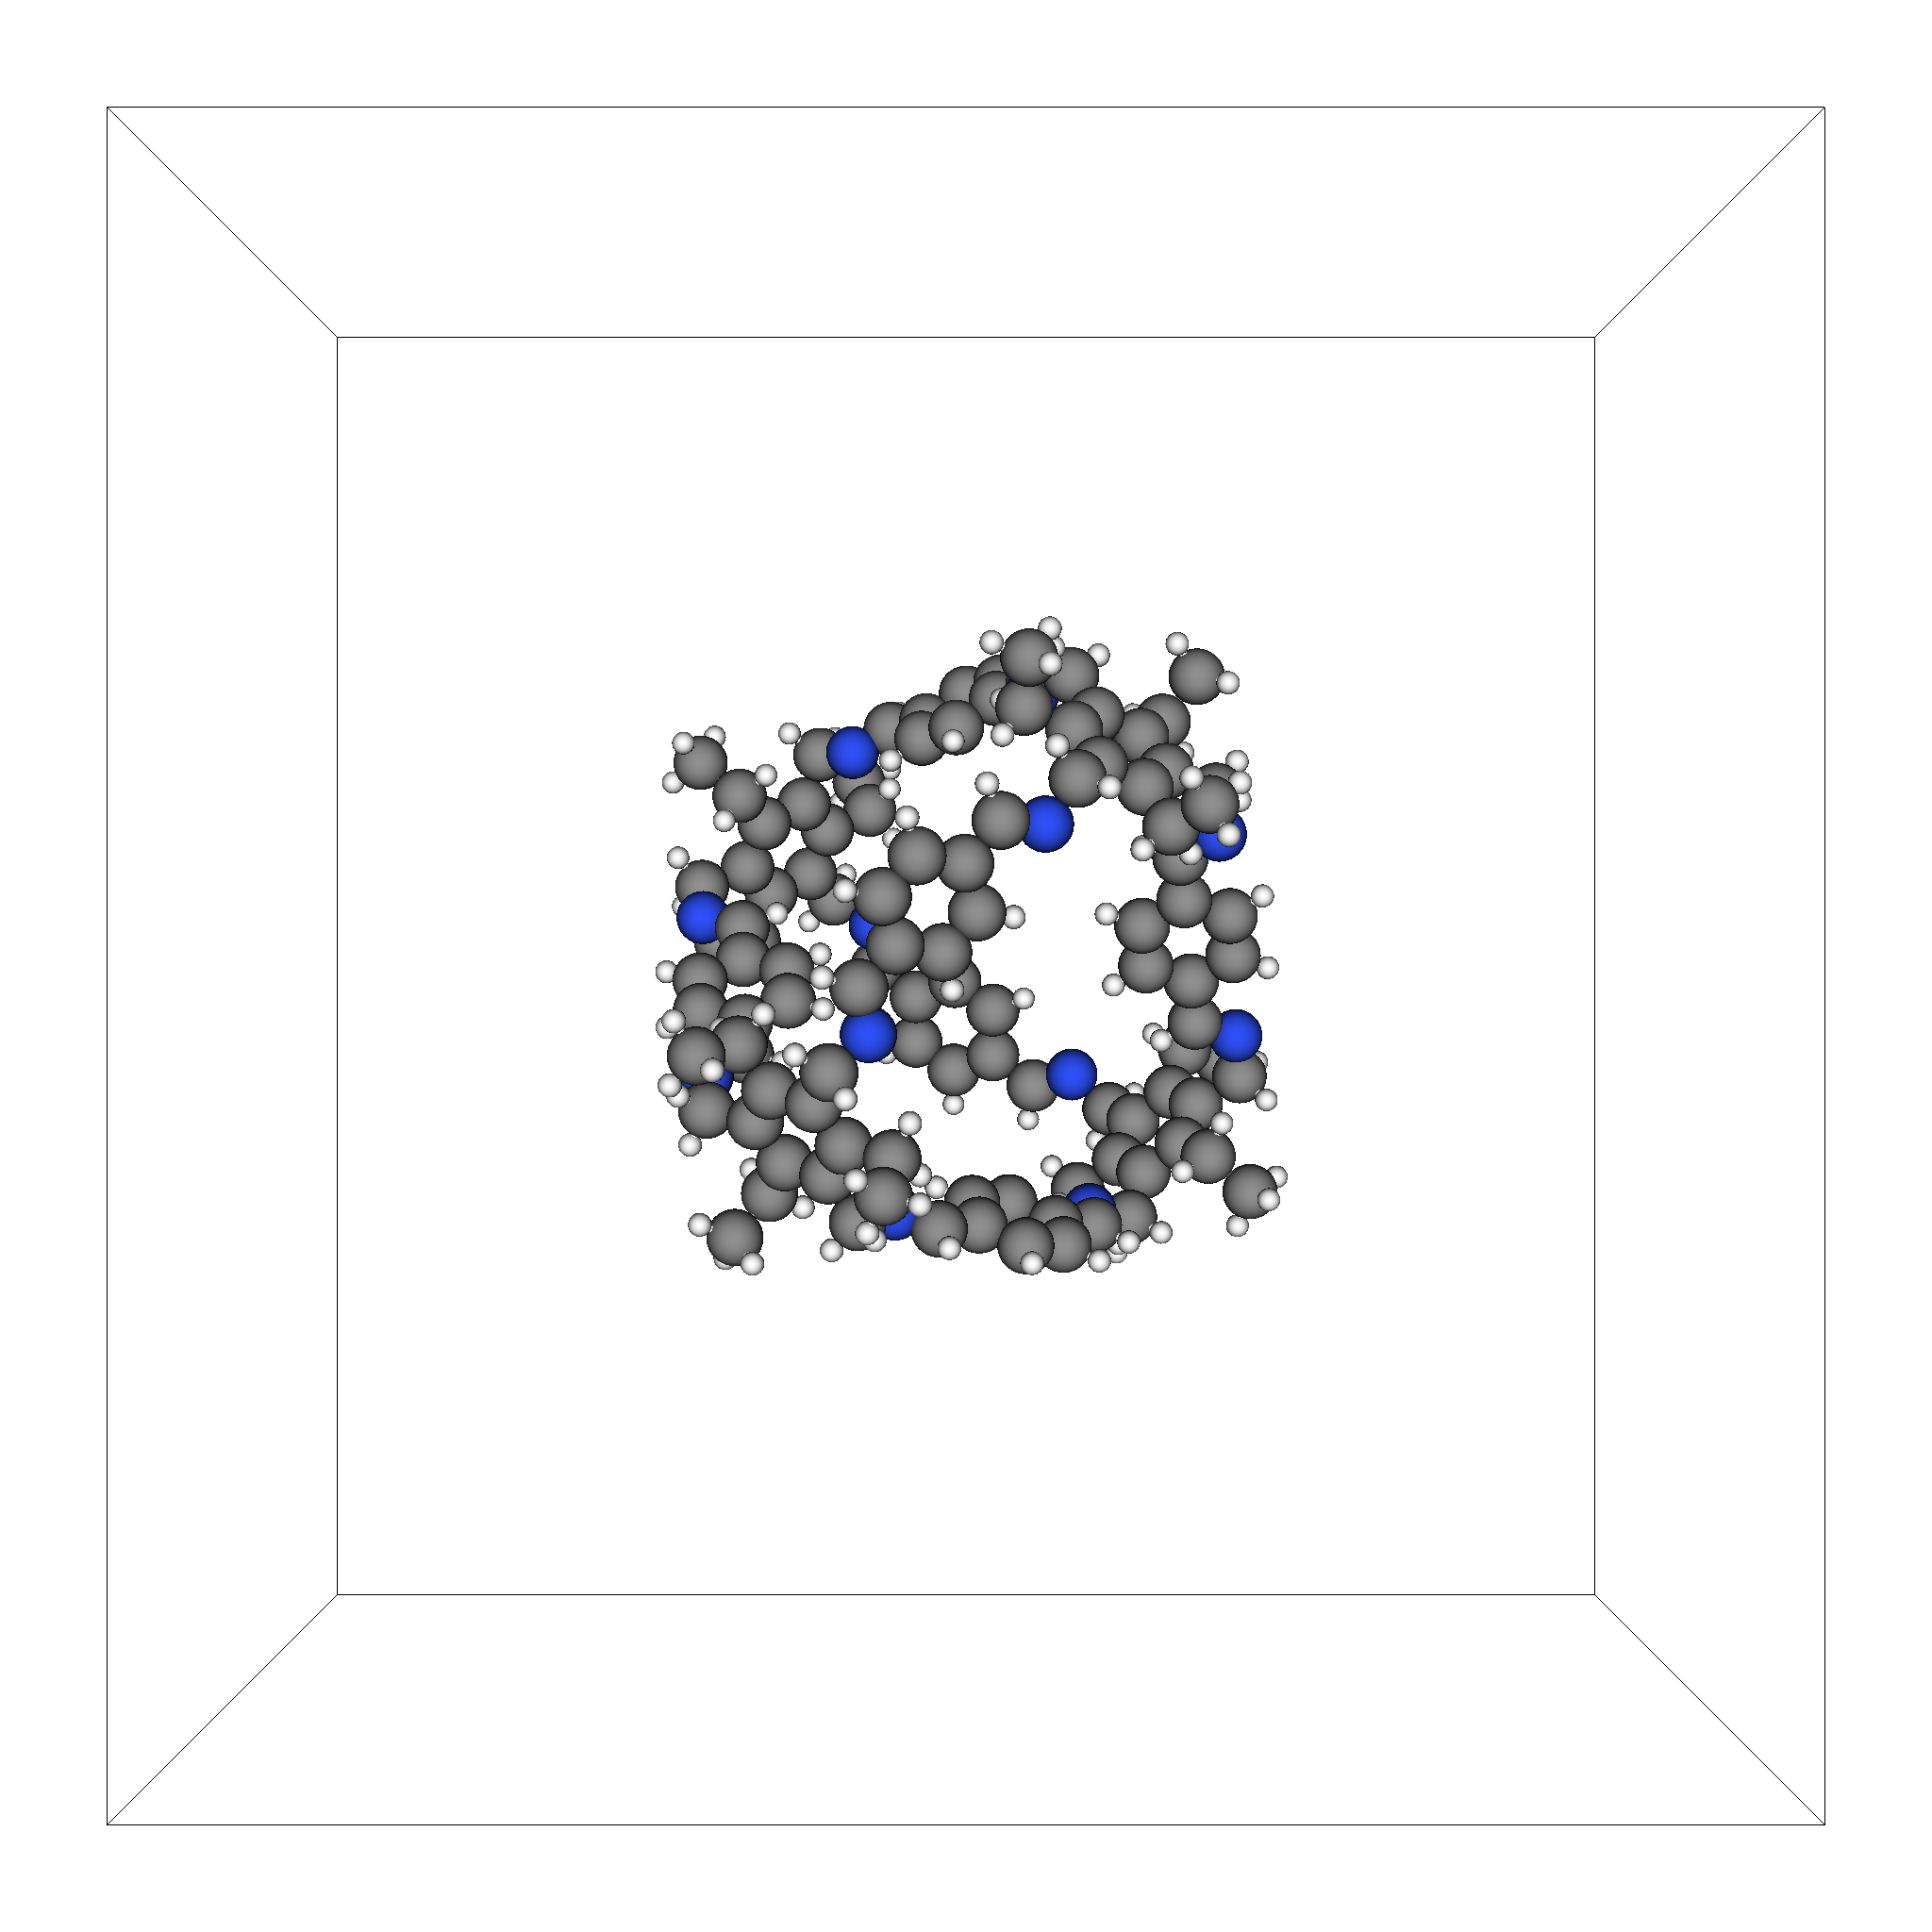
\includegraphics[width=0.25\columnwidth]{../final_aligned_cages/C11.png}}
\subfloat[C13]{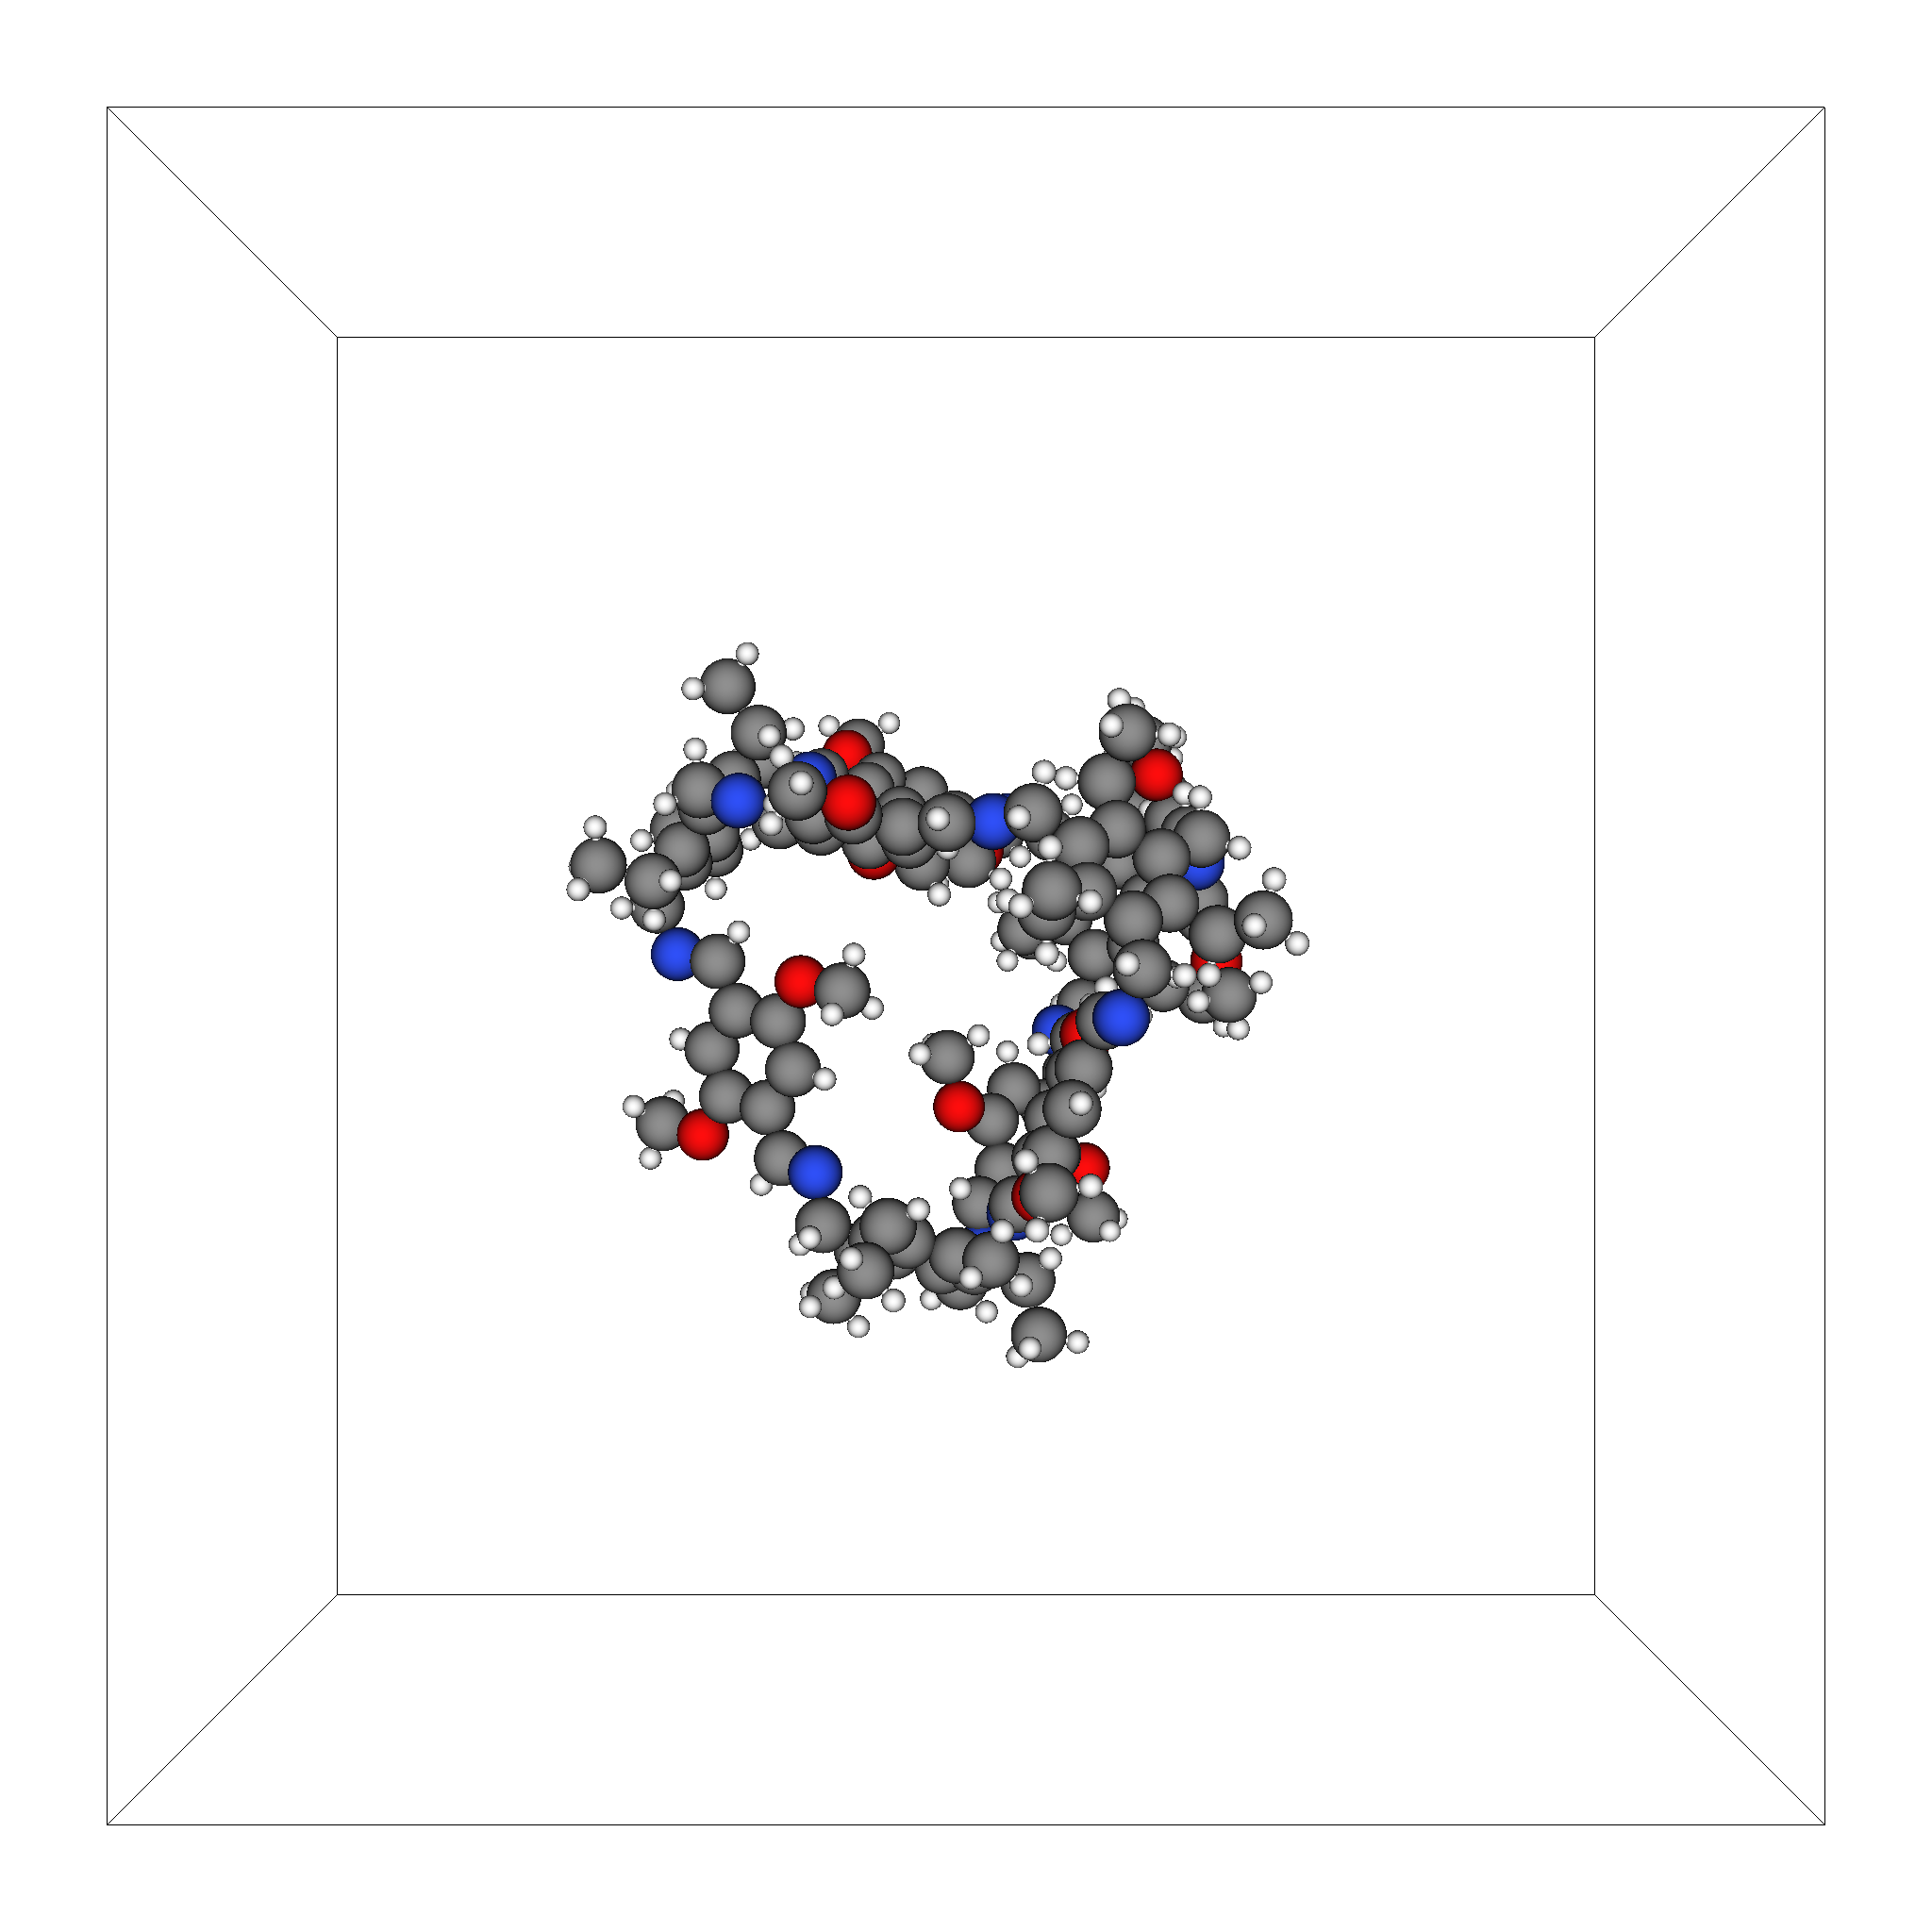
\includegraphics[width=0.25\columnwidth]{../final_aligned_cages/C13.png}}
\qquad
\subfloat[C15]{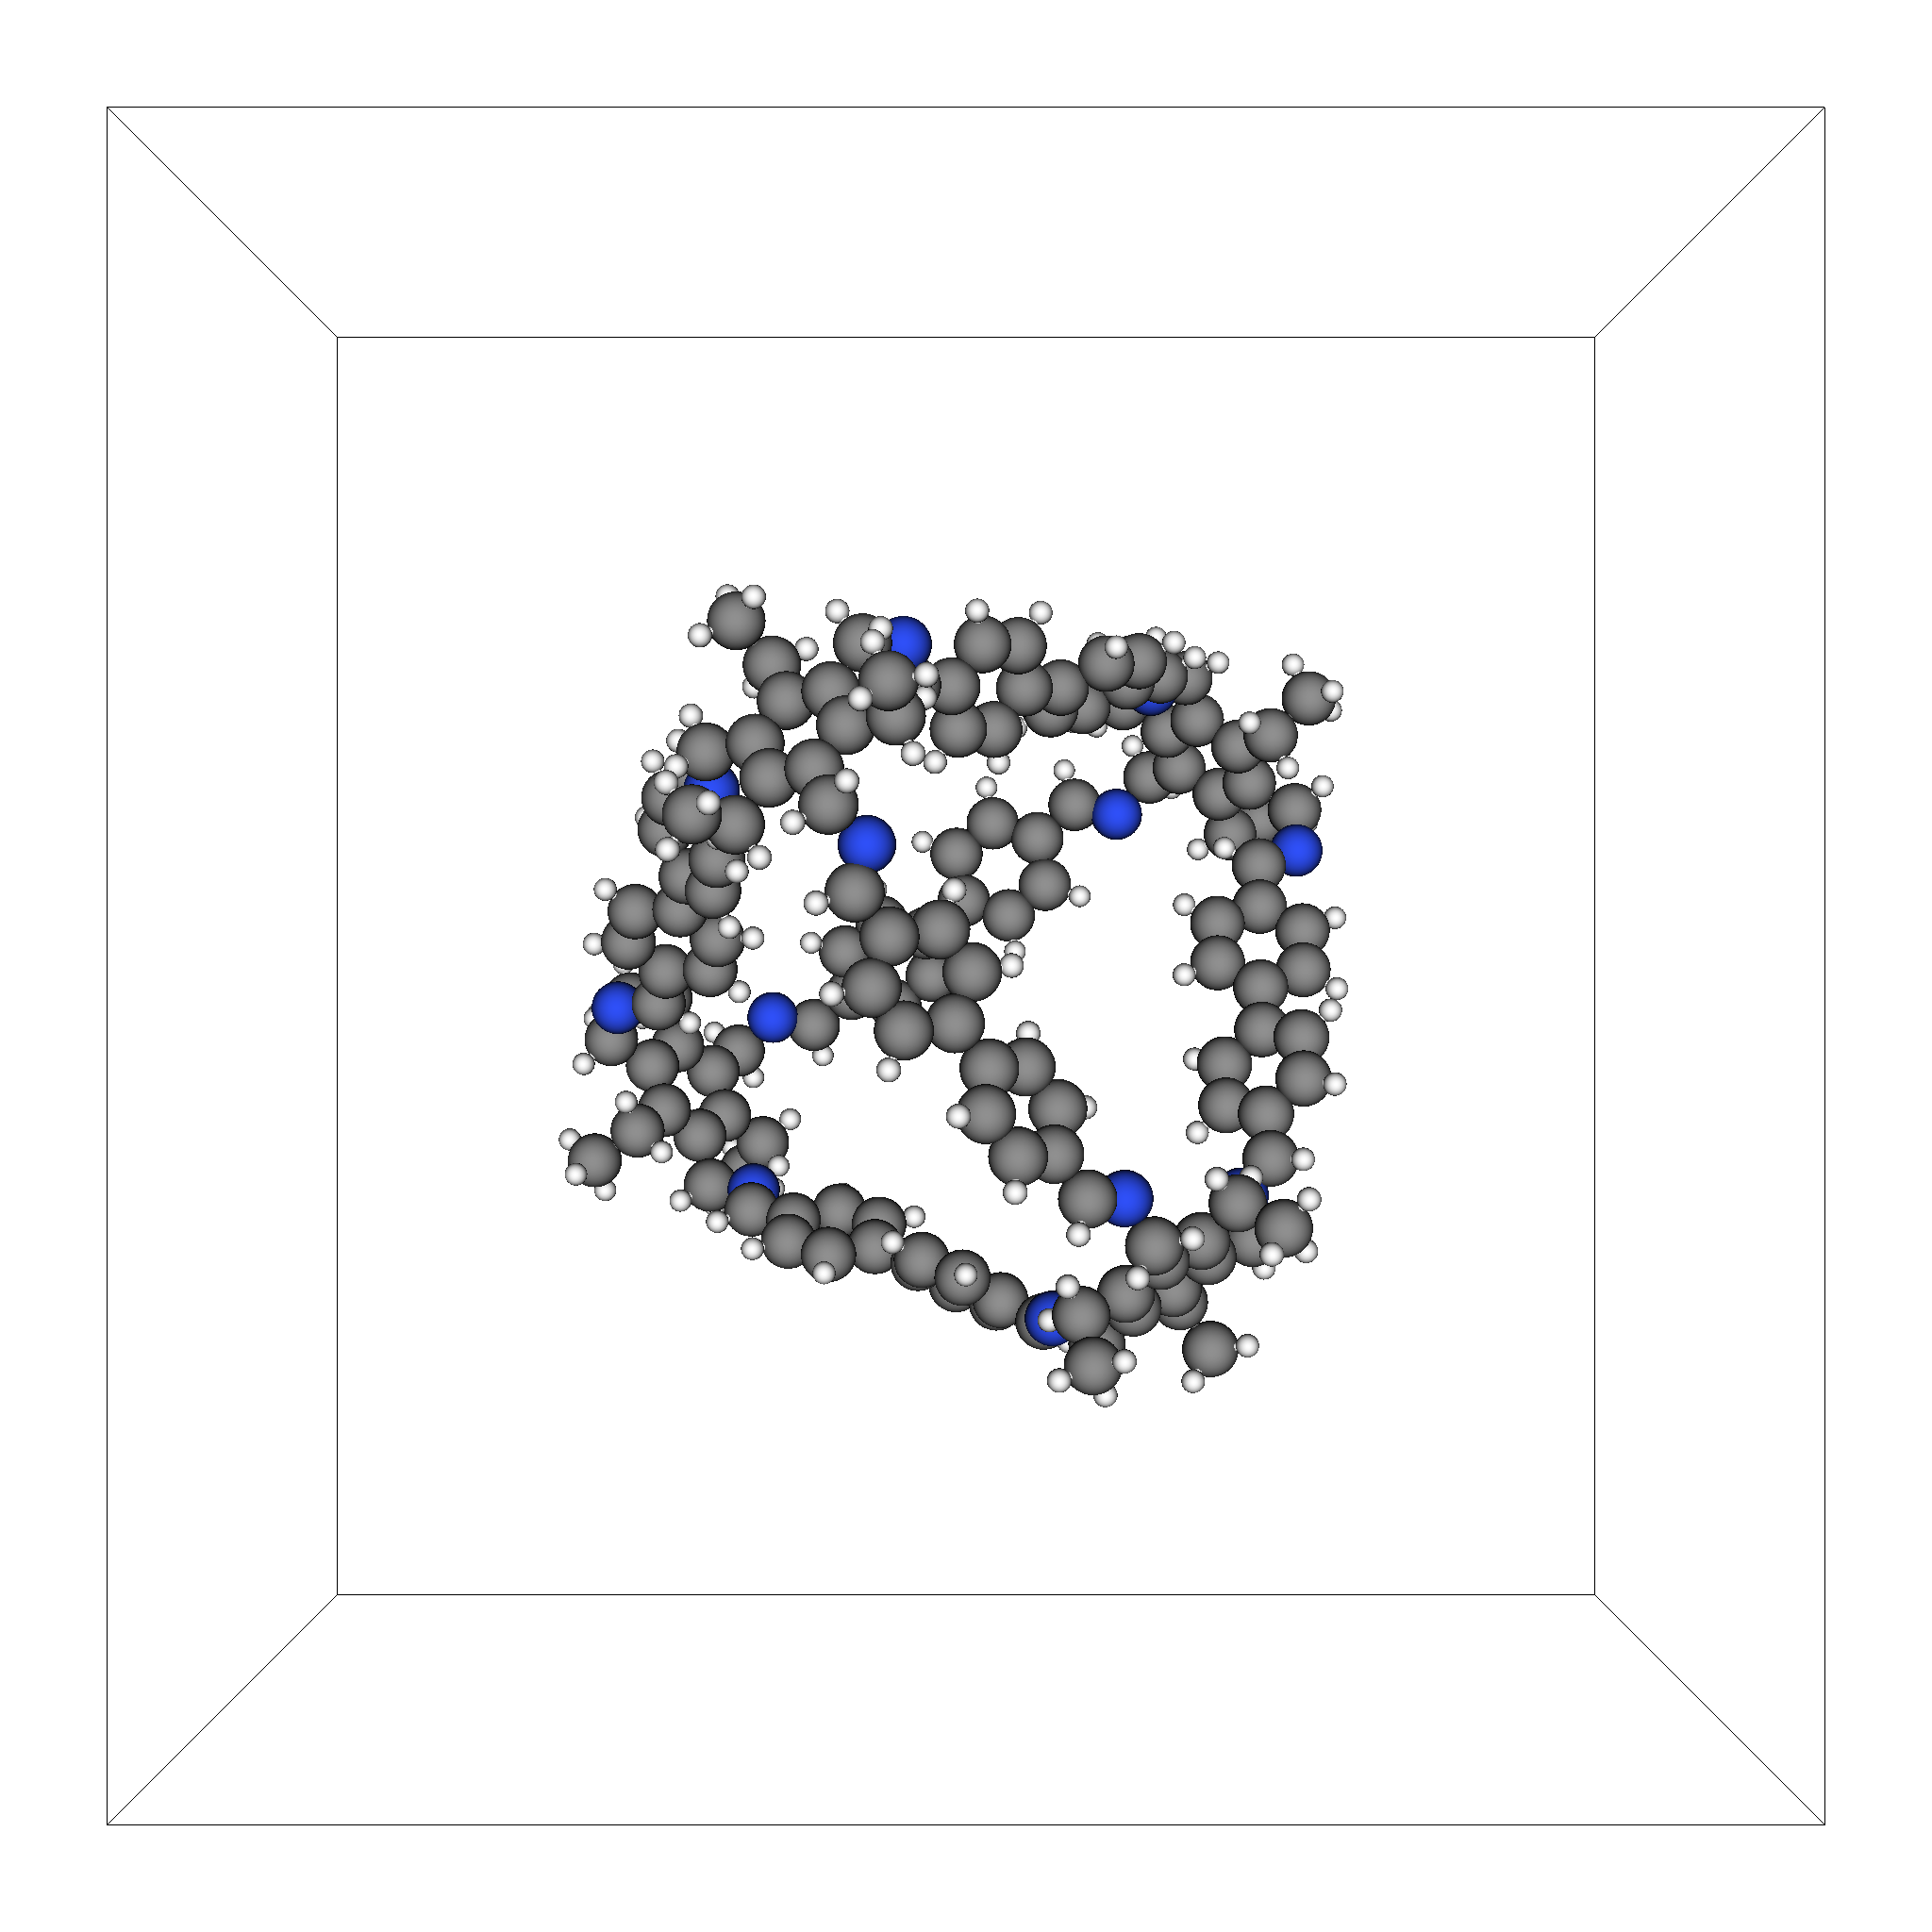
\includegraphics[width=0.25\columnwidth]{../final_aligned_cages/C15.png}}
\subfloat[C18]{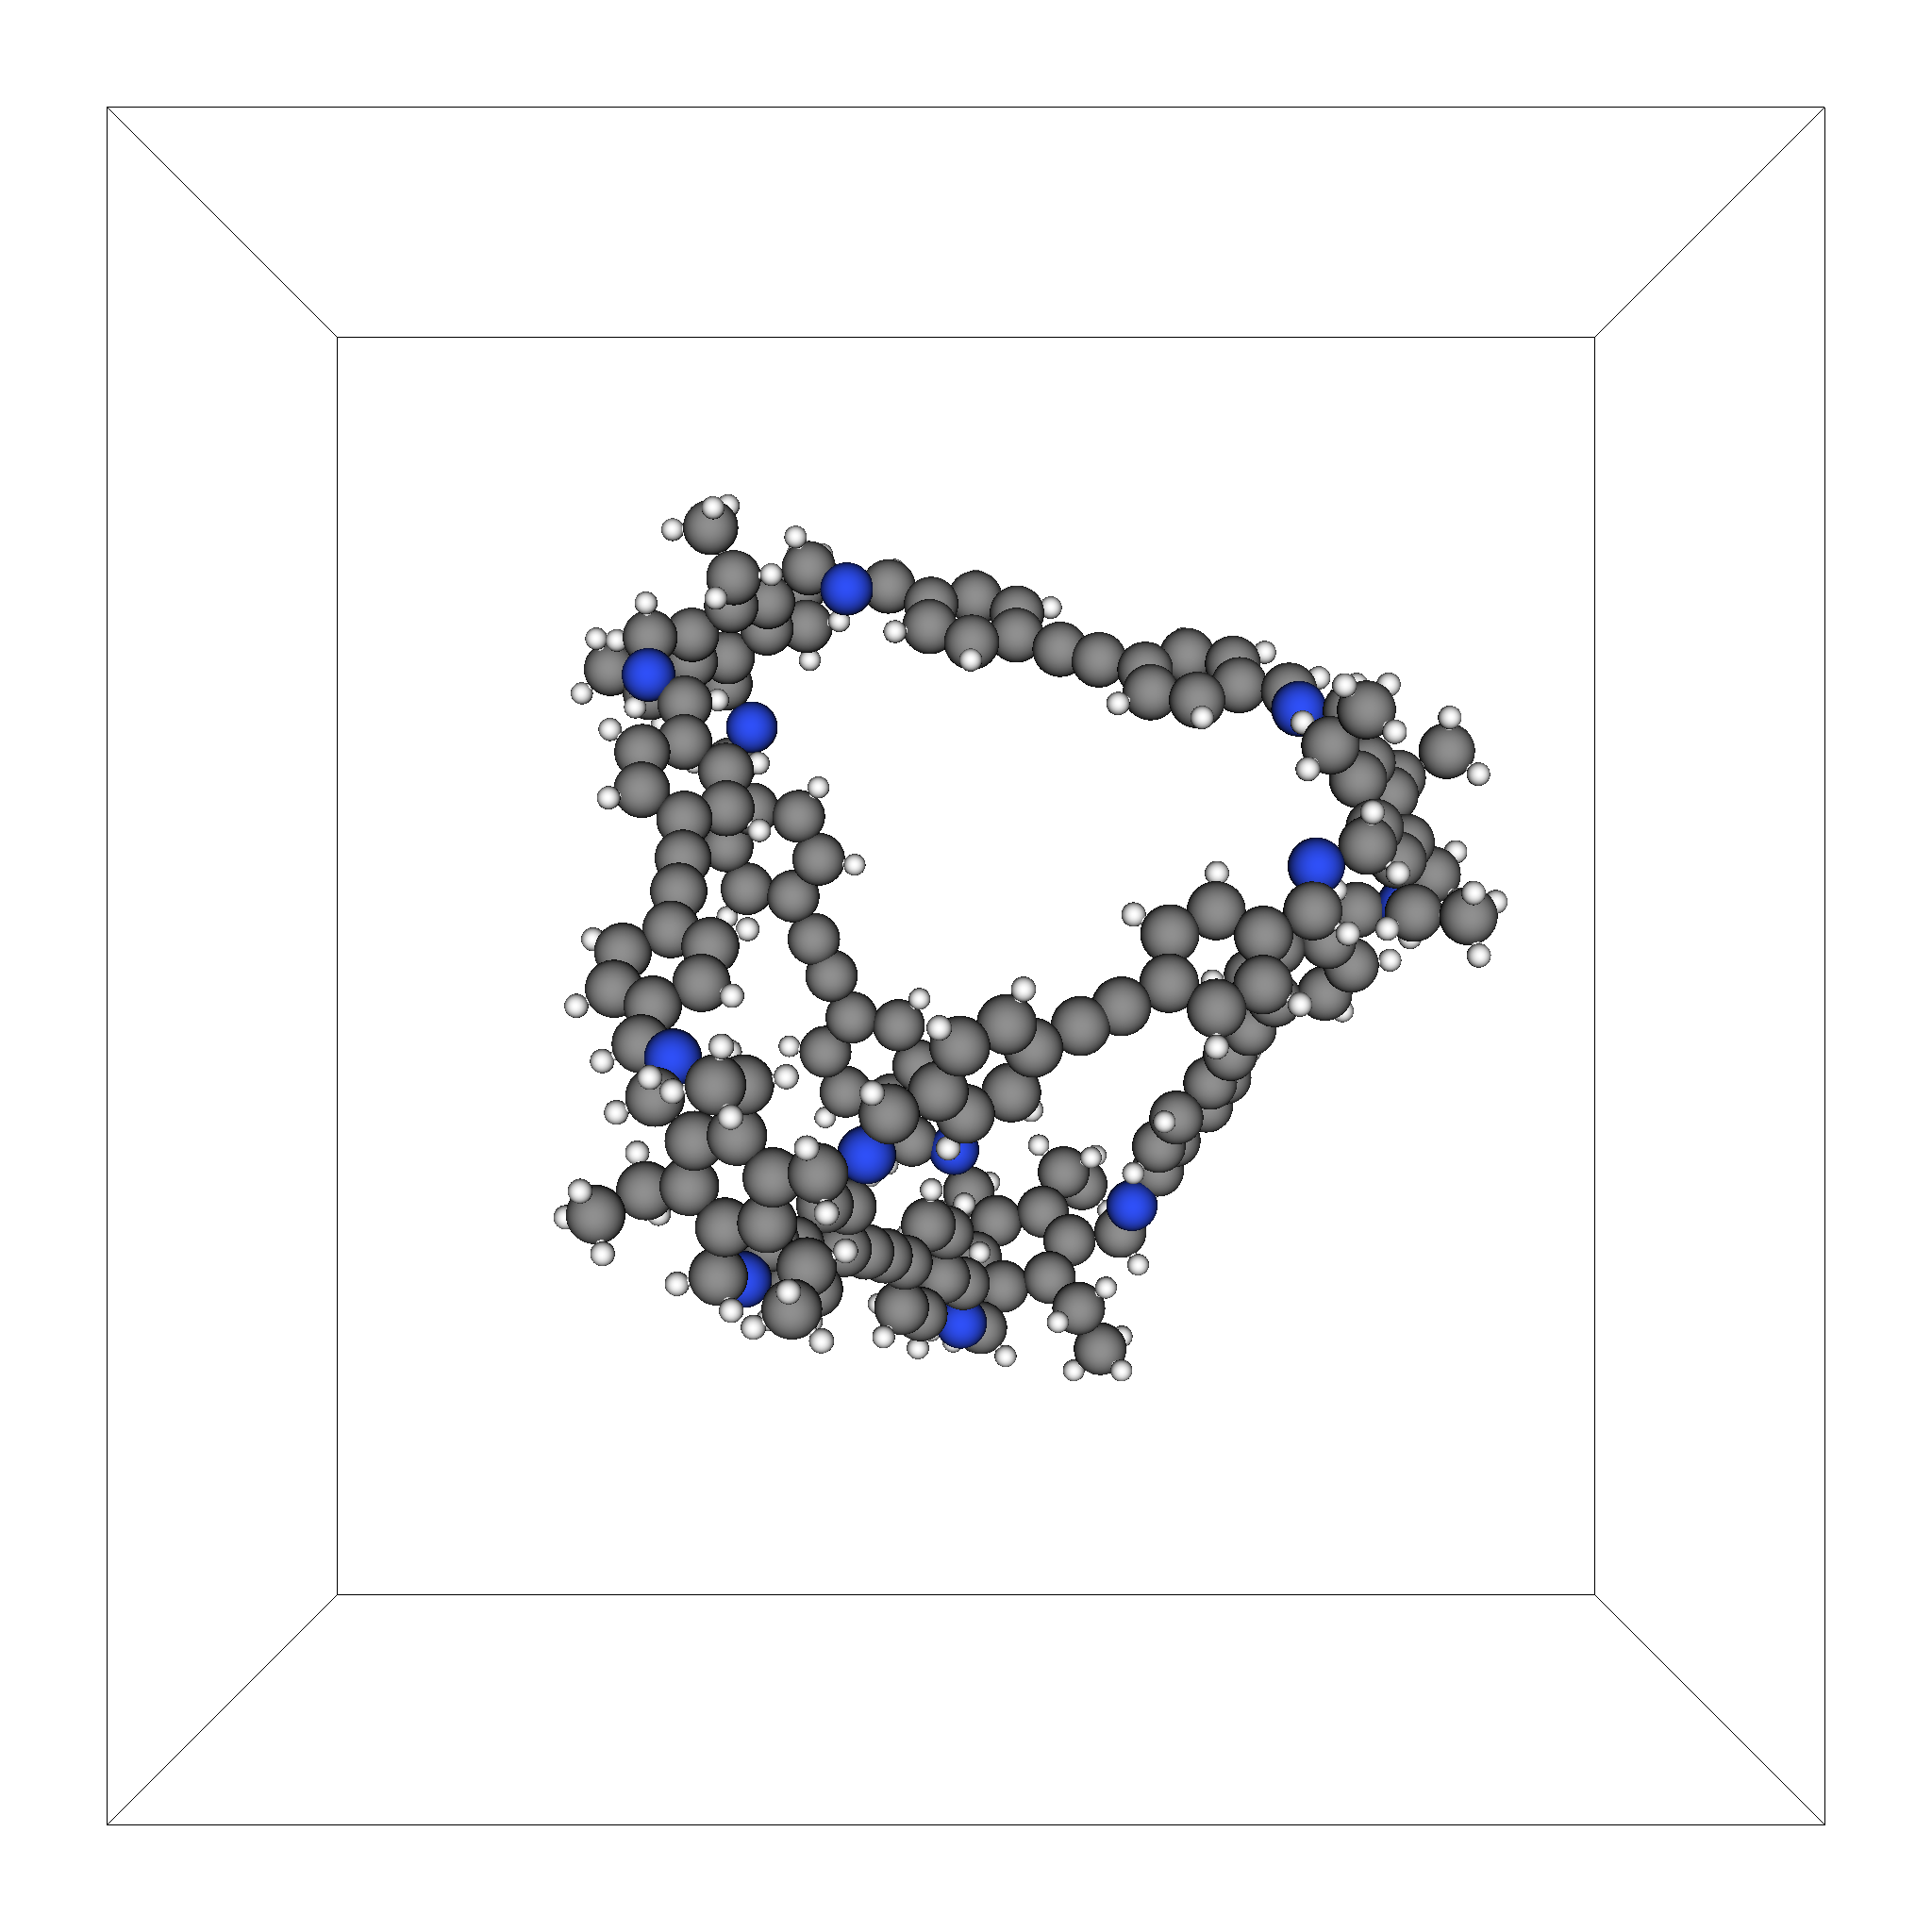
\includegraphics[width=0.25\columnwidth]{../final_aligned_cages/C18.png}}
\subfloat[C1]{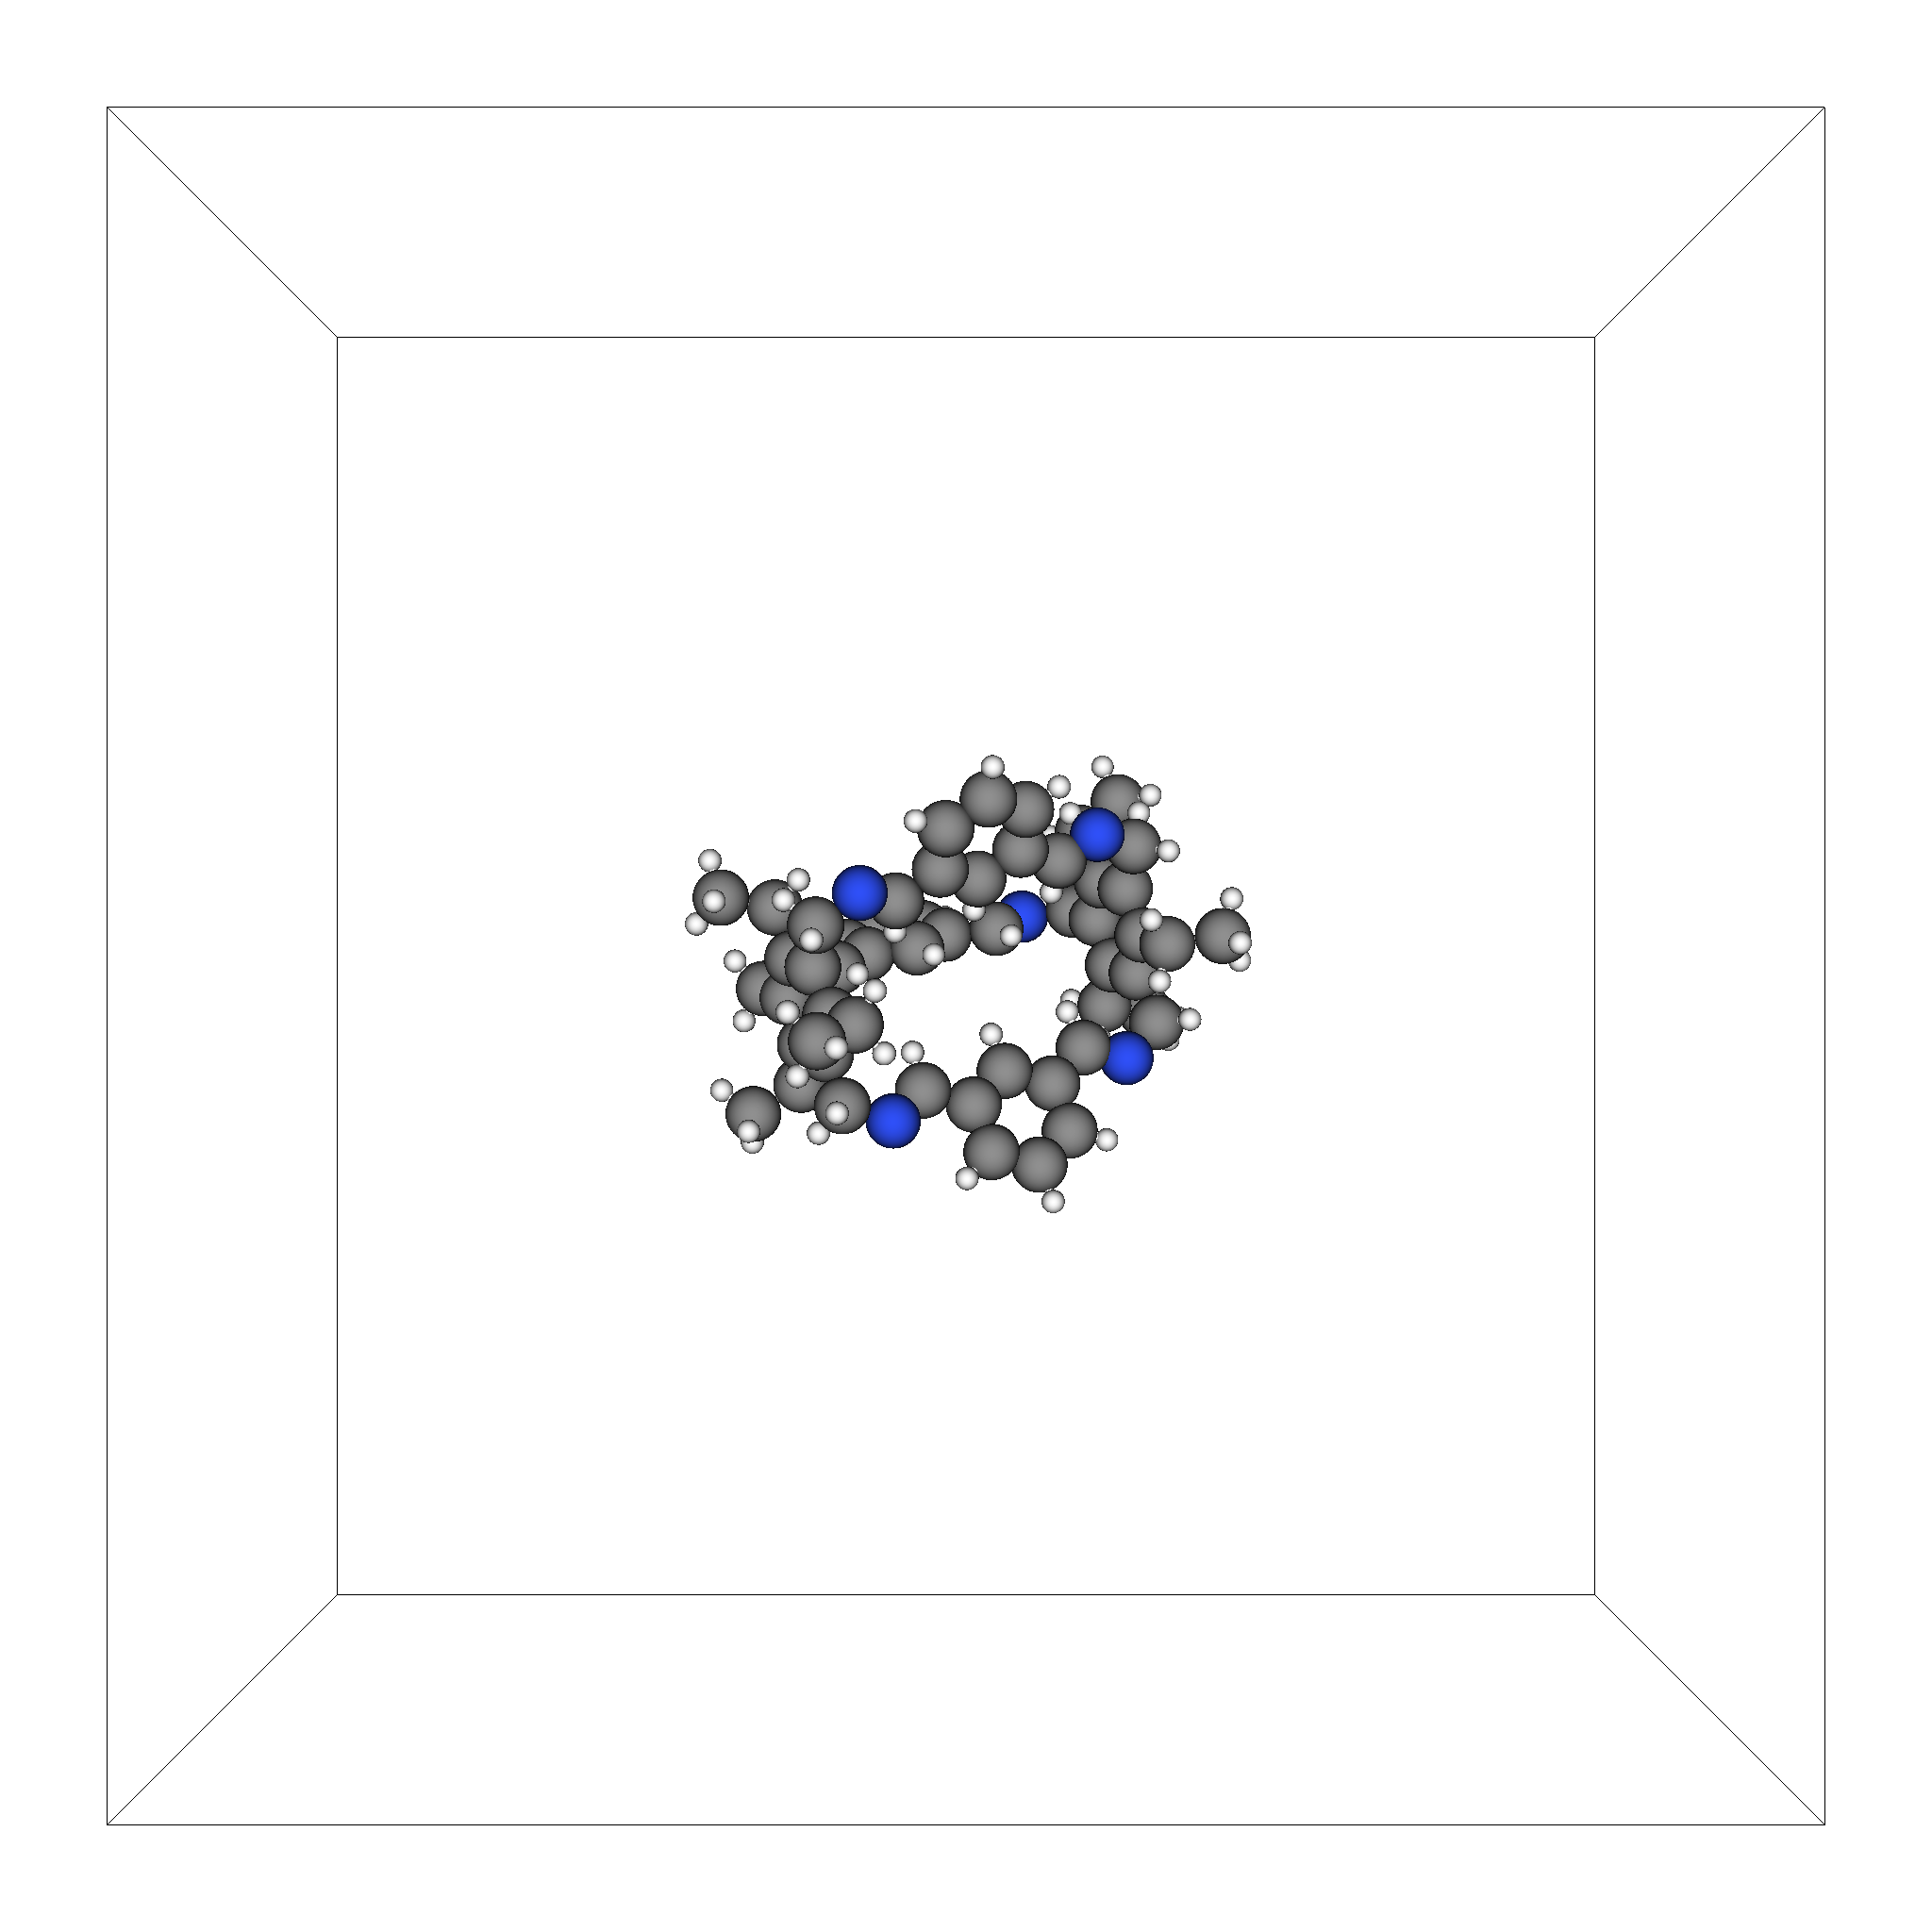
\includegraphics[width=0.25\columnwidth]{../final_aligned_cages/C1.png}}
\qquad
\subfloat[C20]{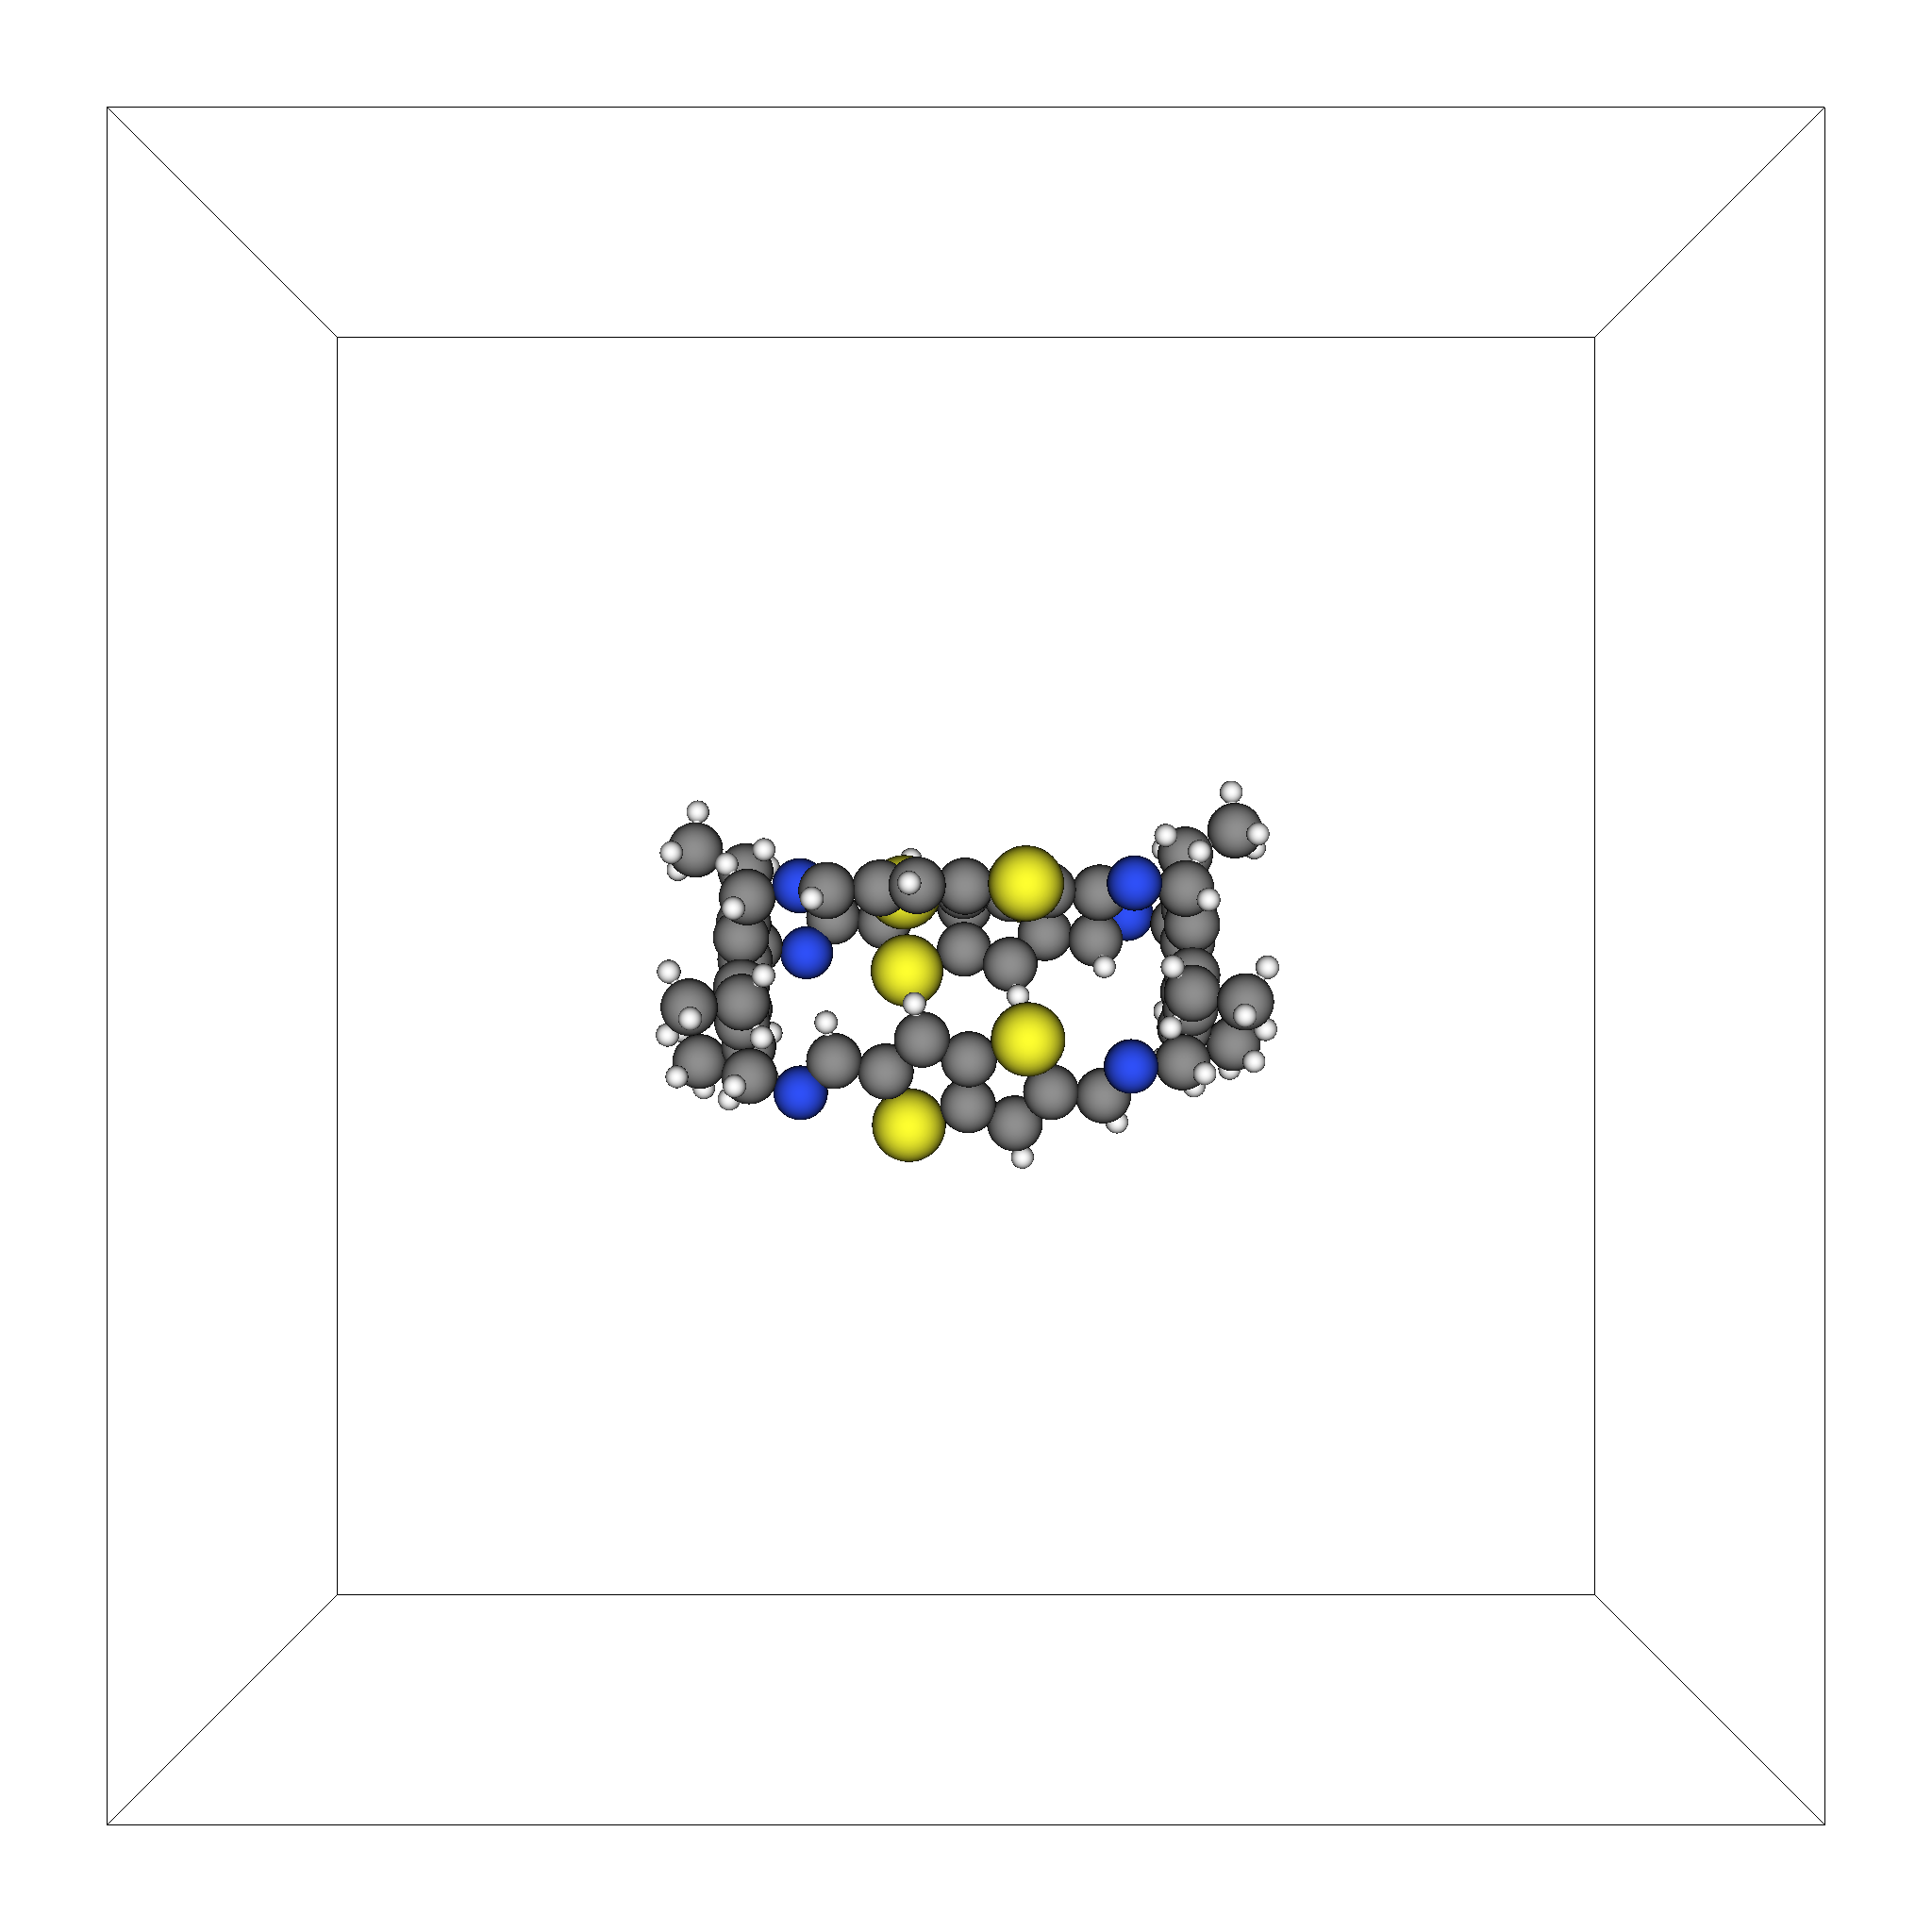
\includegraphics[width=0.25\columnwidth]{../final_aligned_cages/C20.png}}
\subfloat[C21]{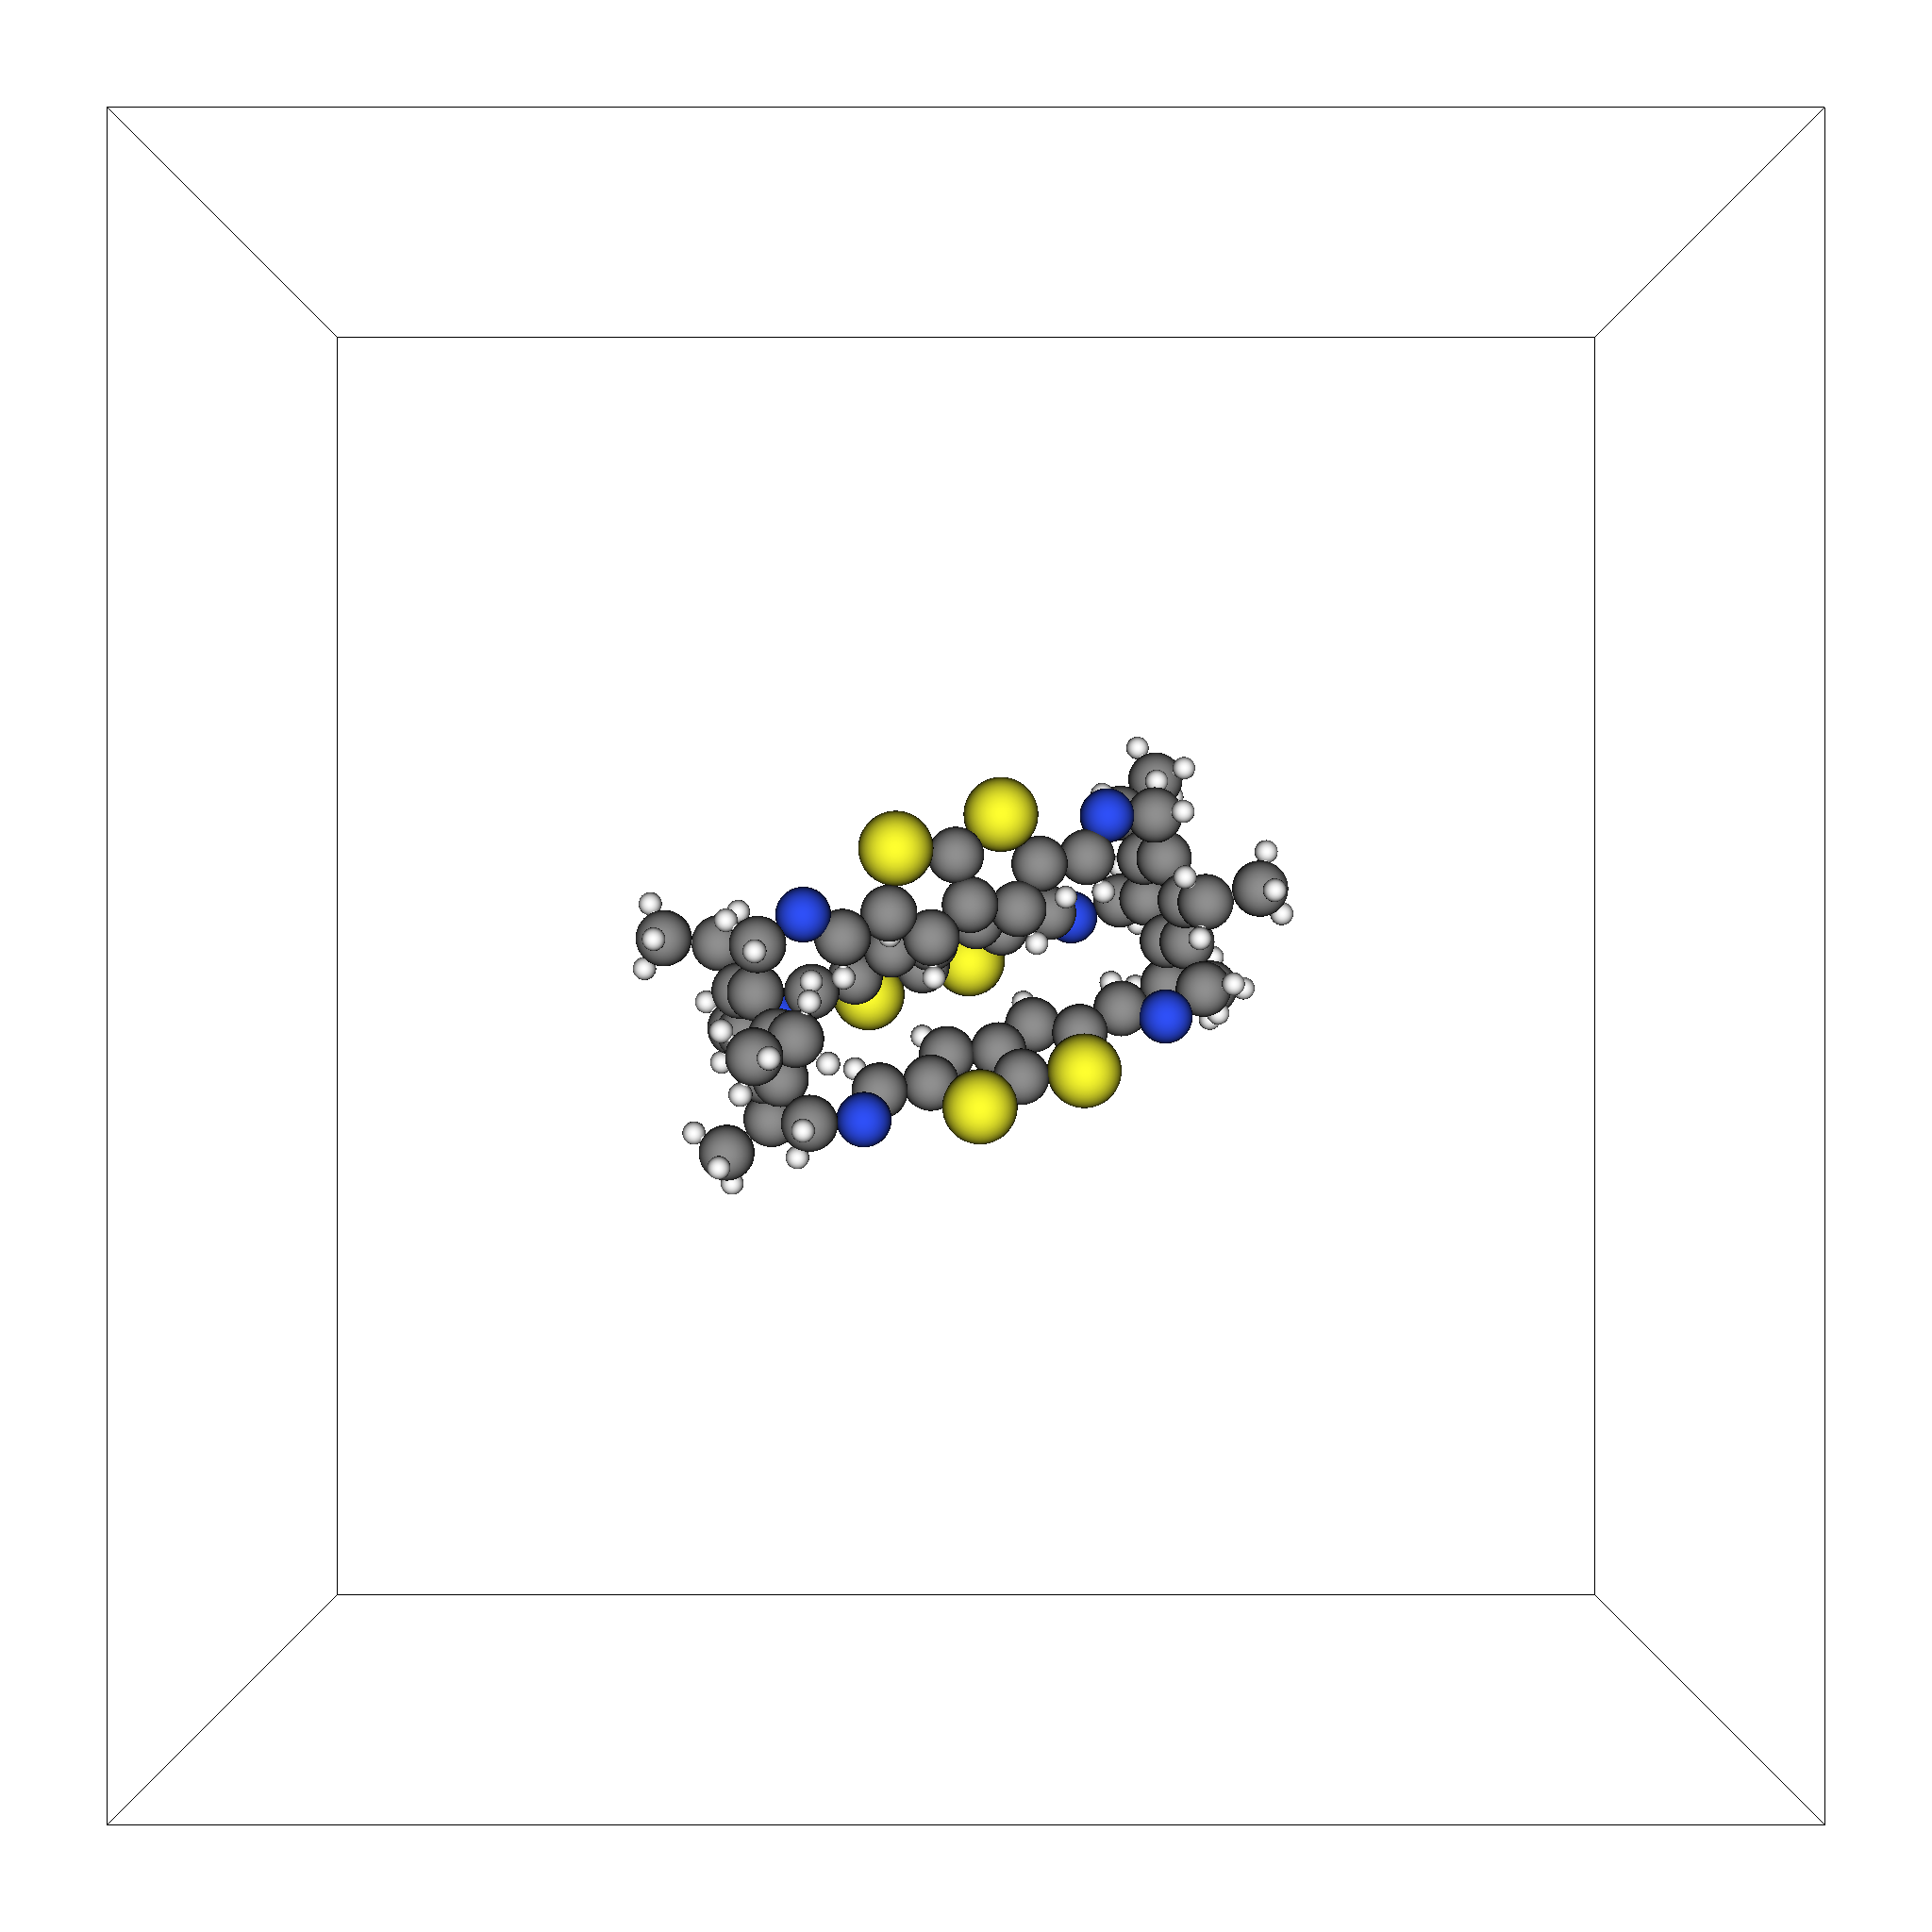
\includegraphics[width=0.25\columnwidth]{../final_aligned_cages/C21.png}}
\subfloat[C23]{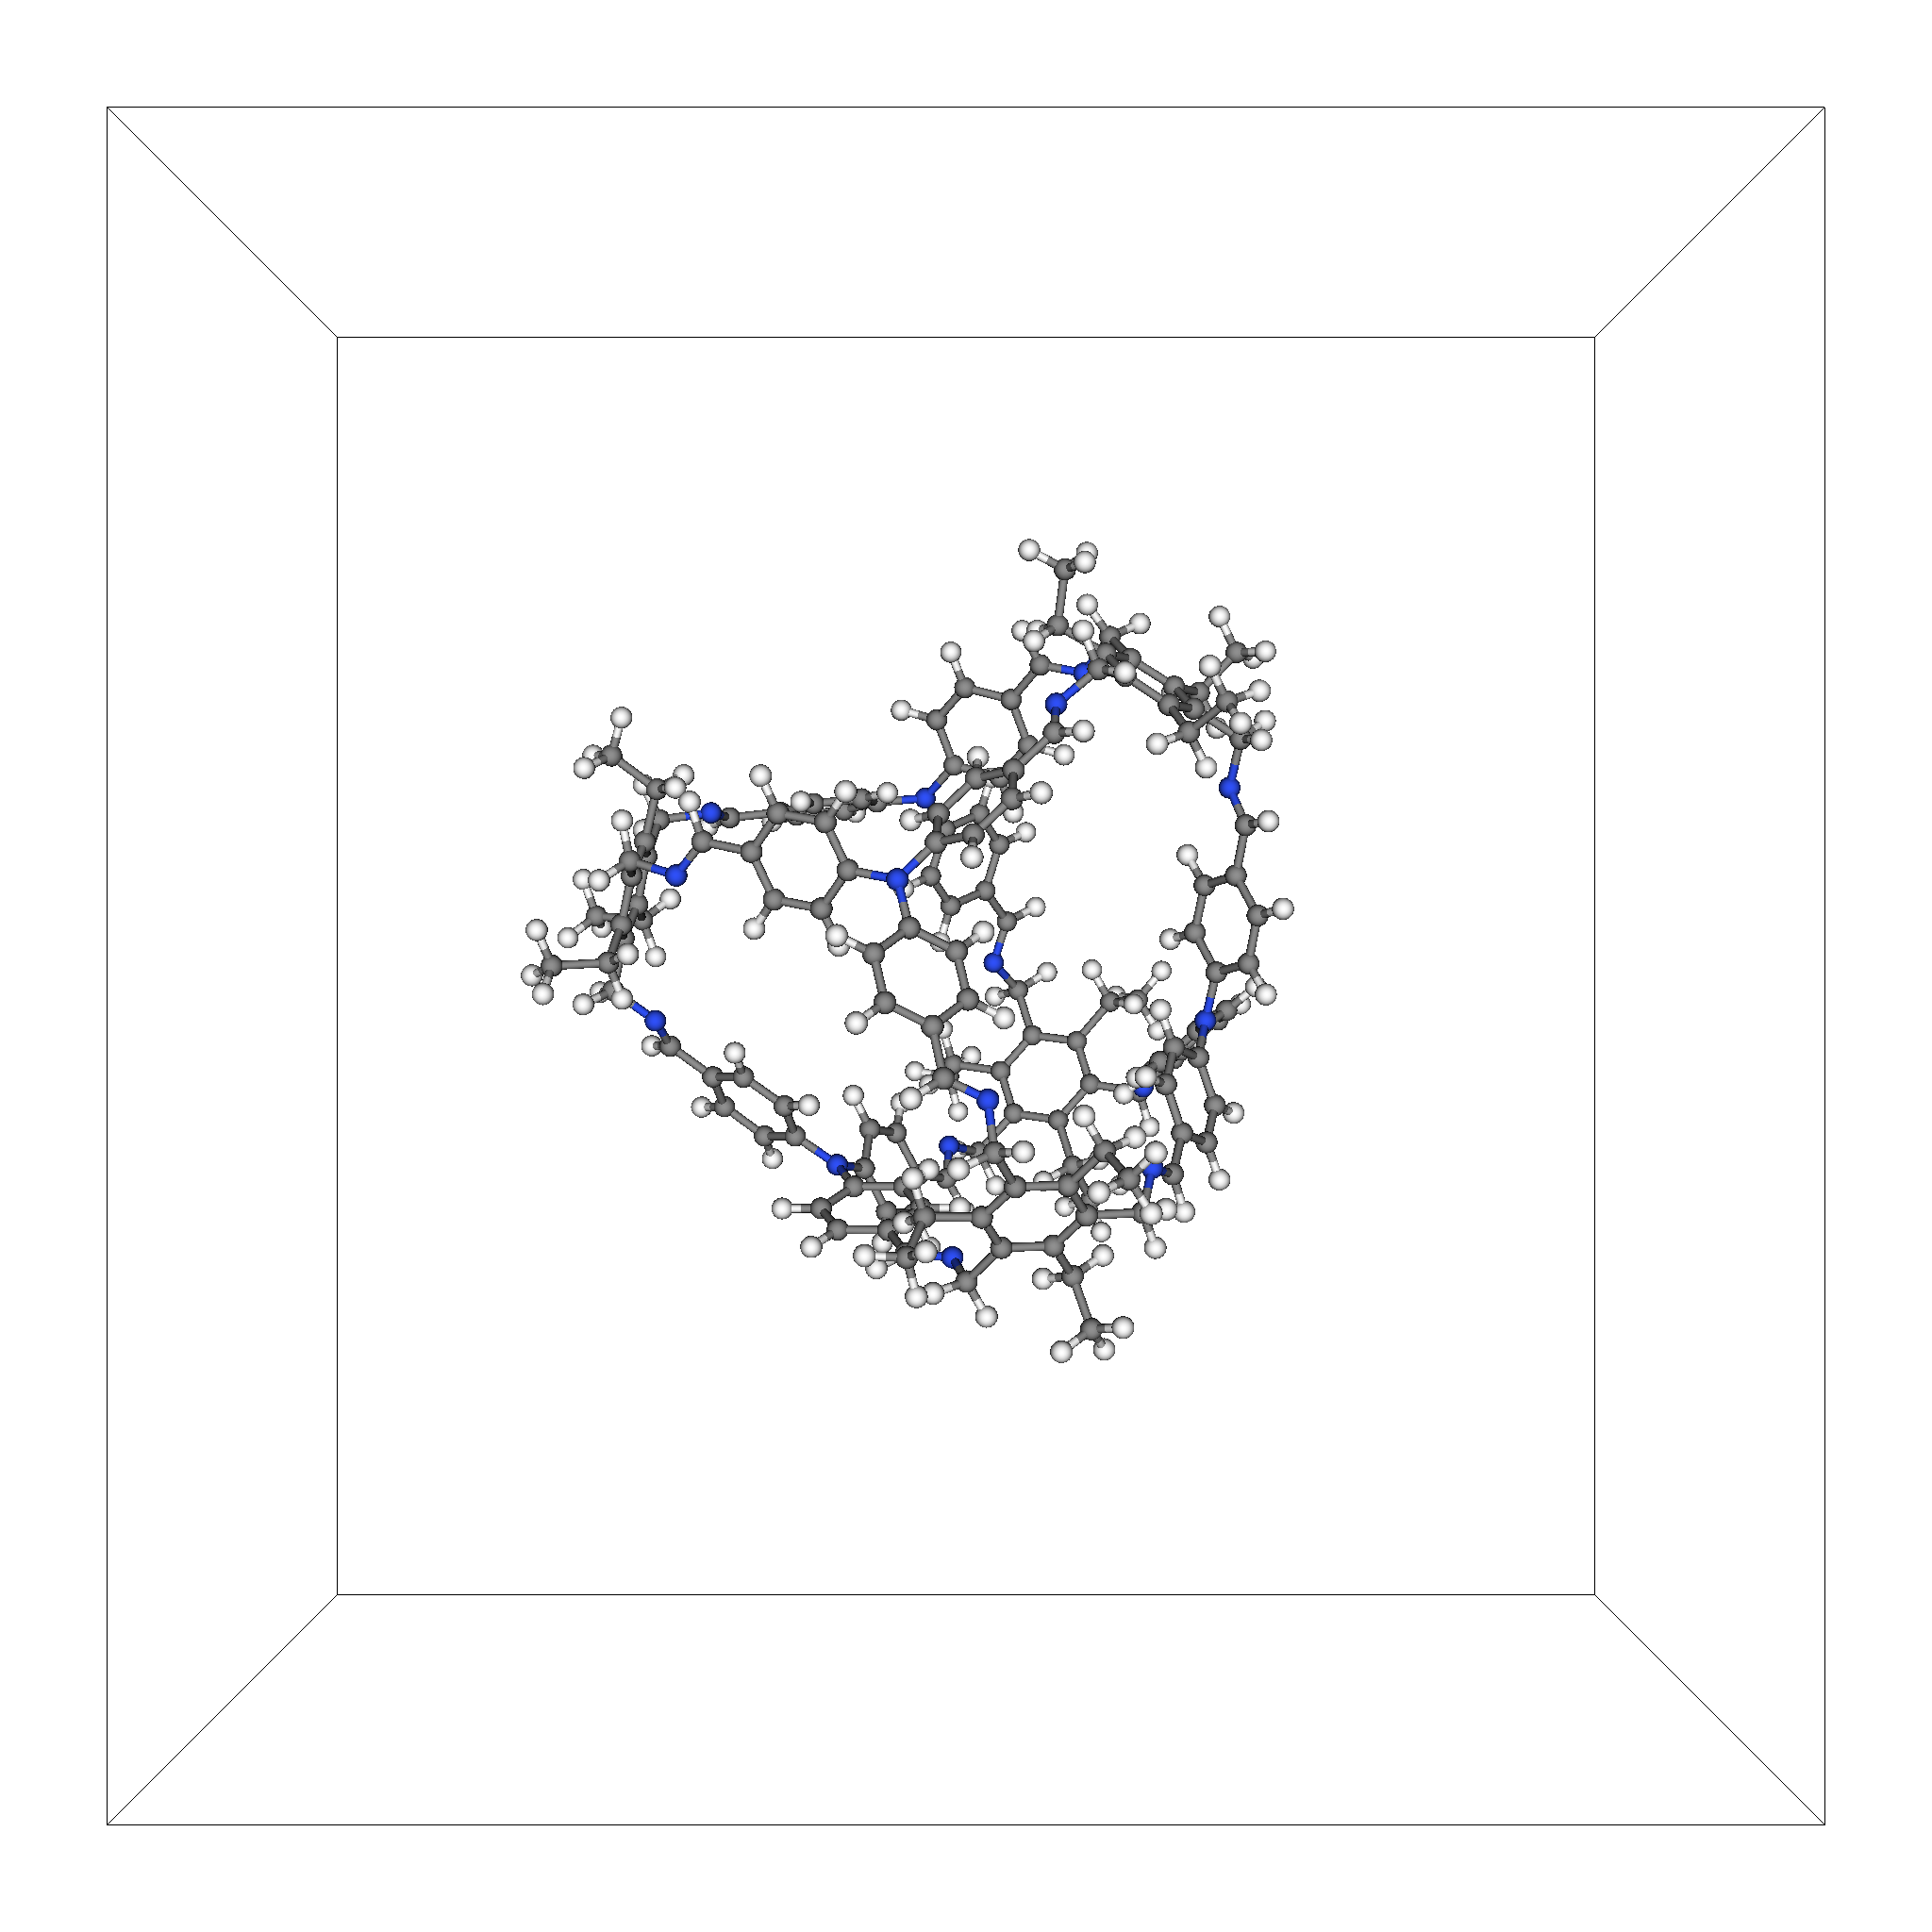
\includegraphics[width=0.25\columnwidth]{../final_aligned_cages/C23.png}}
\phantomcaption \end{figure}
\begin{figure}
\ContinuedFloat \centering
\subfloat[C24]{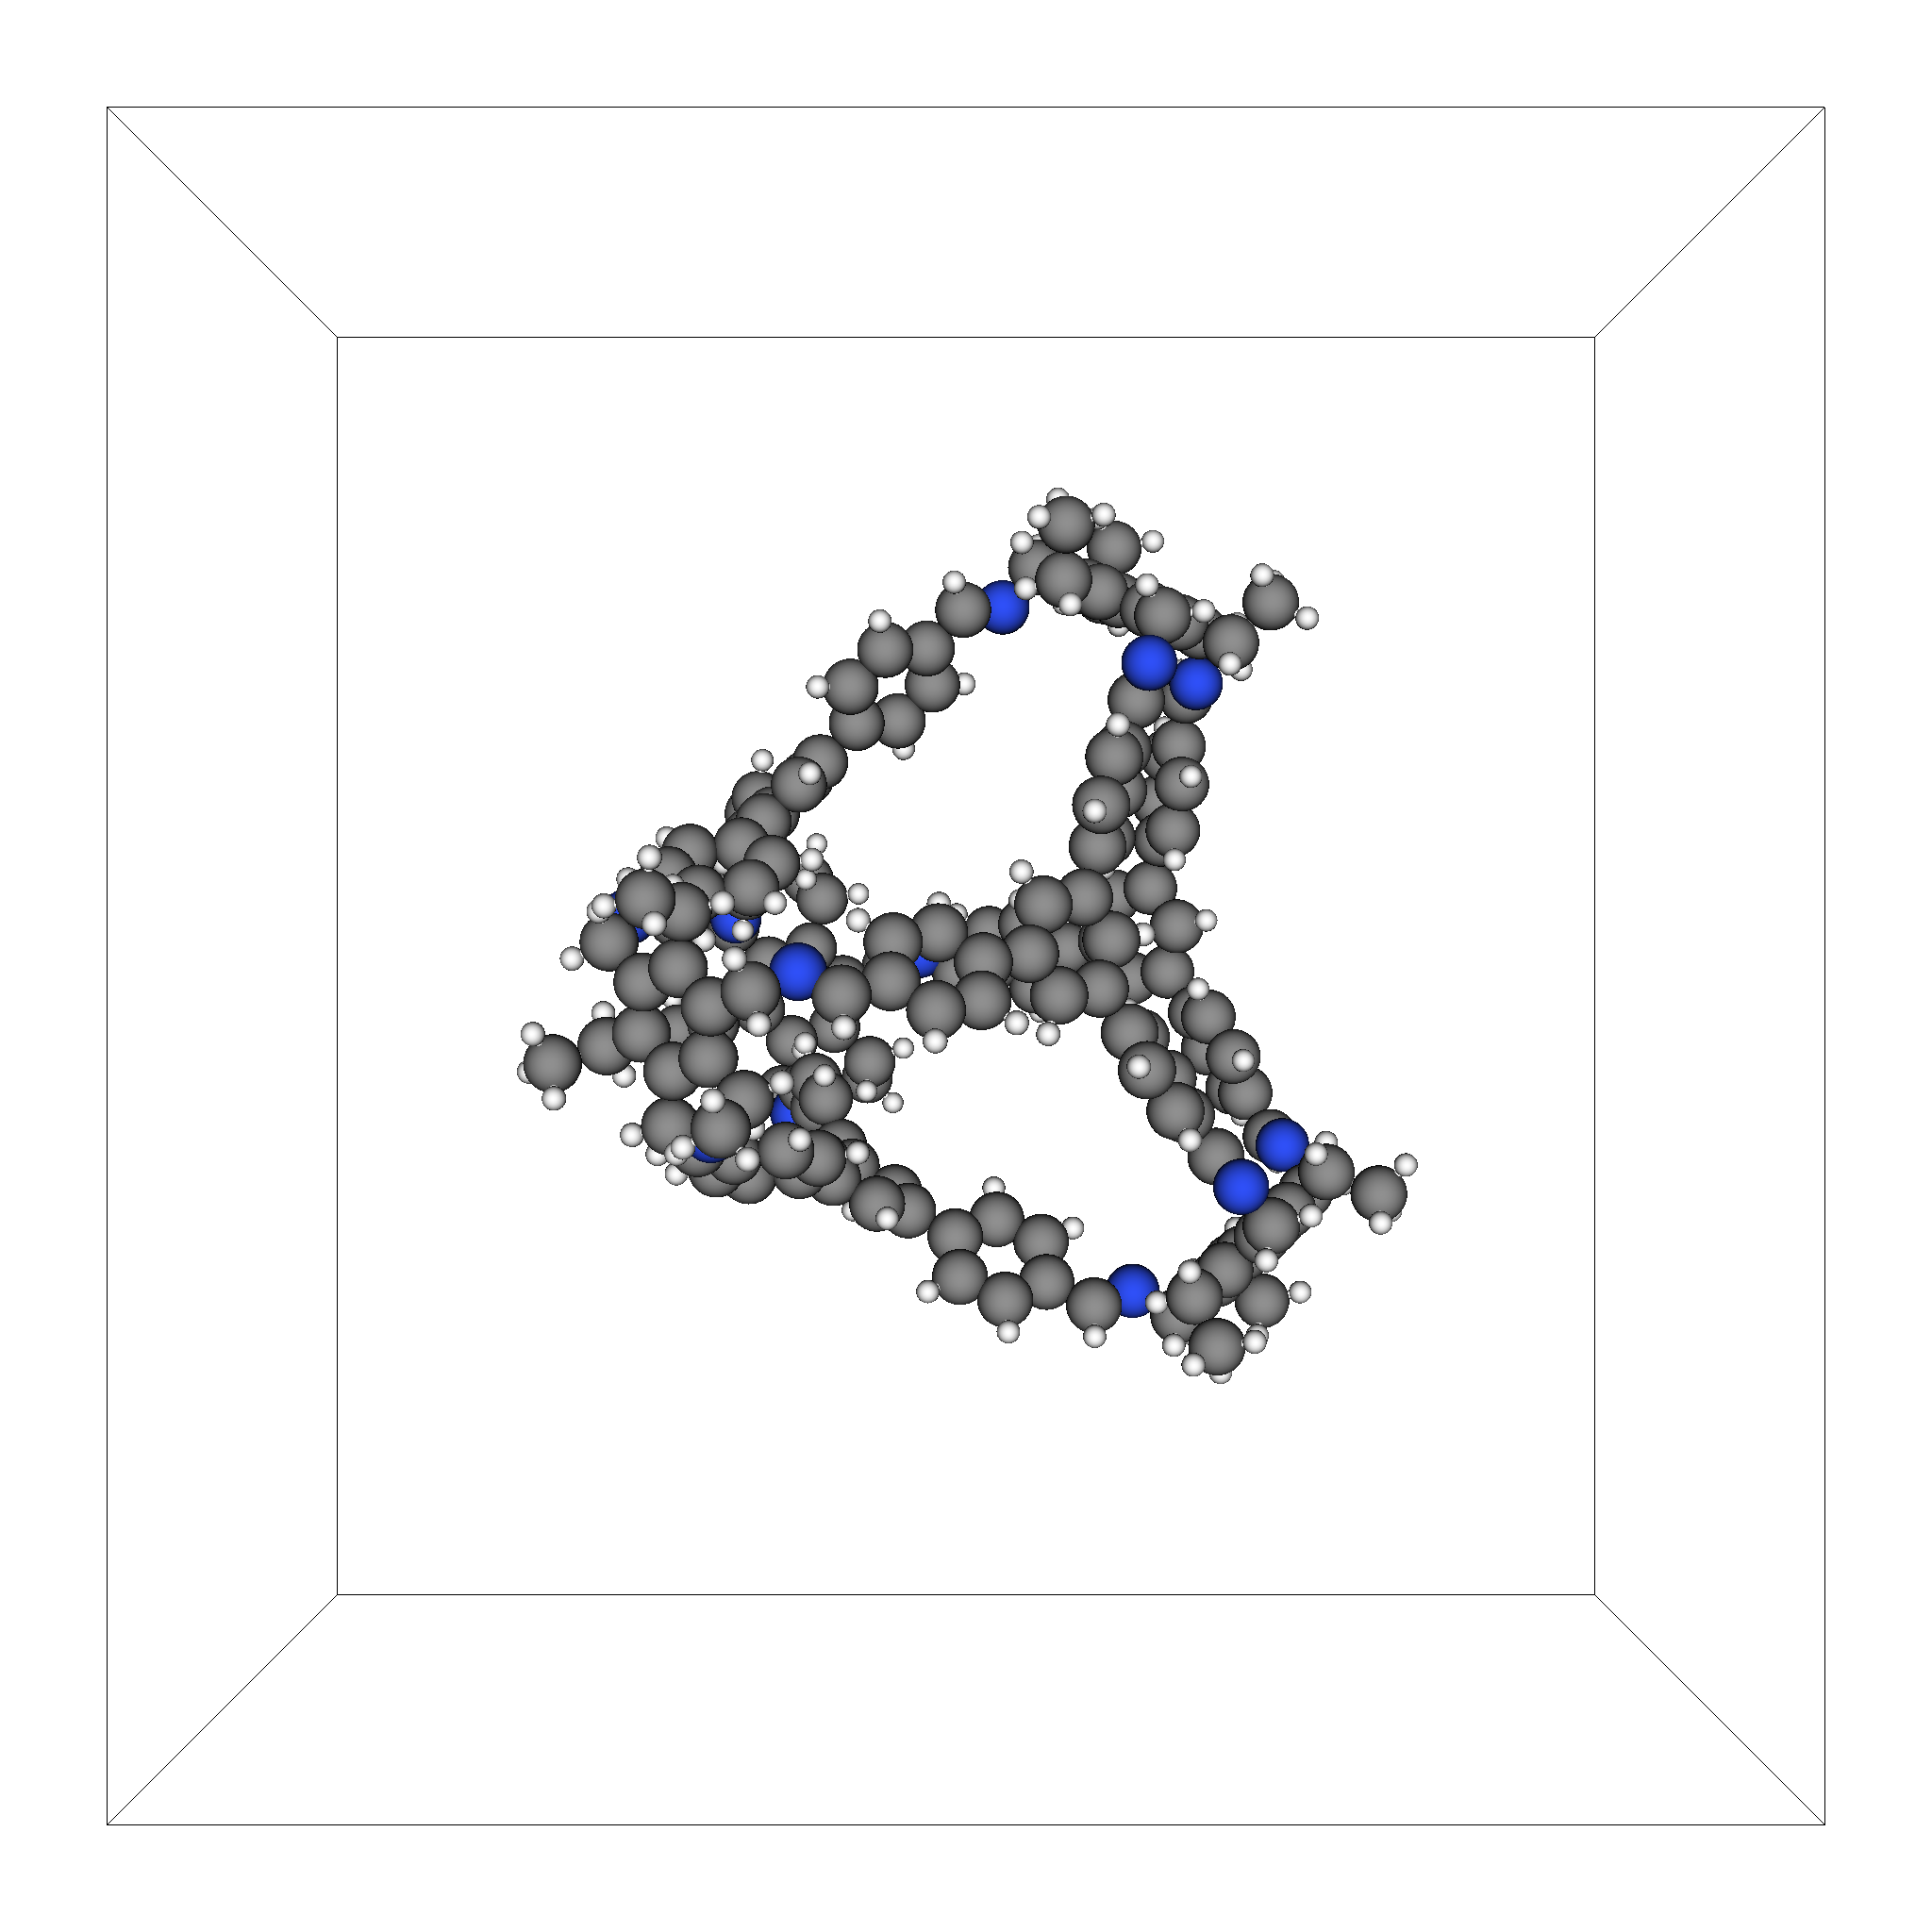
\includegraphics[width=0.25\columnwidth]{../final_aligned_cages/C24.png}}
\subfloat[C25]{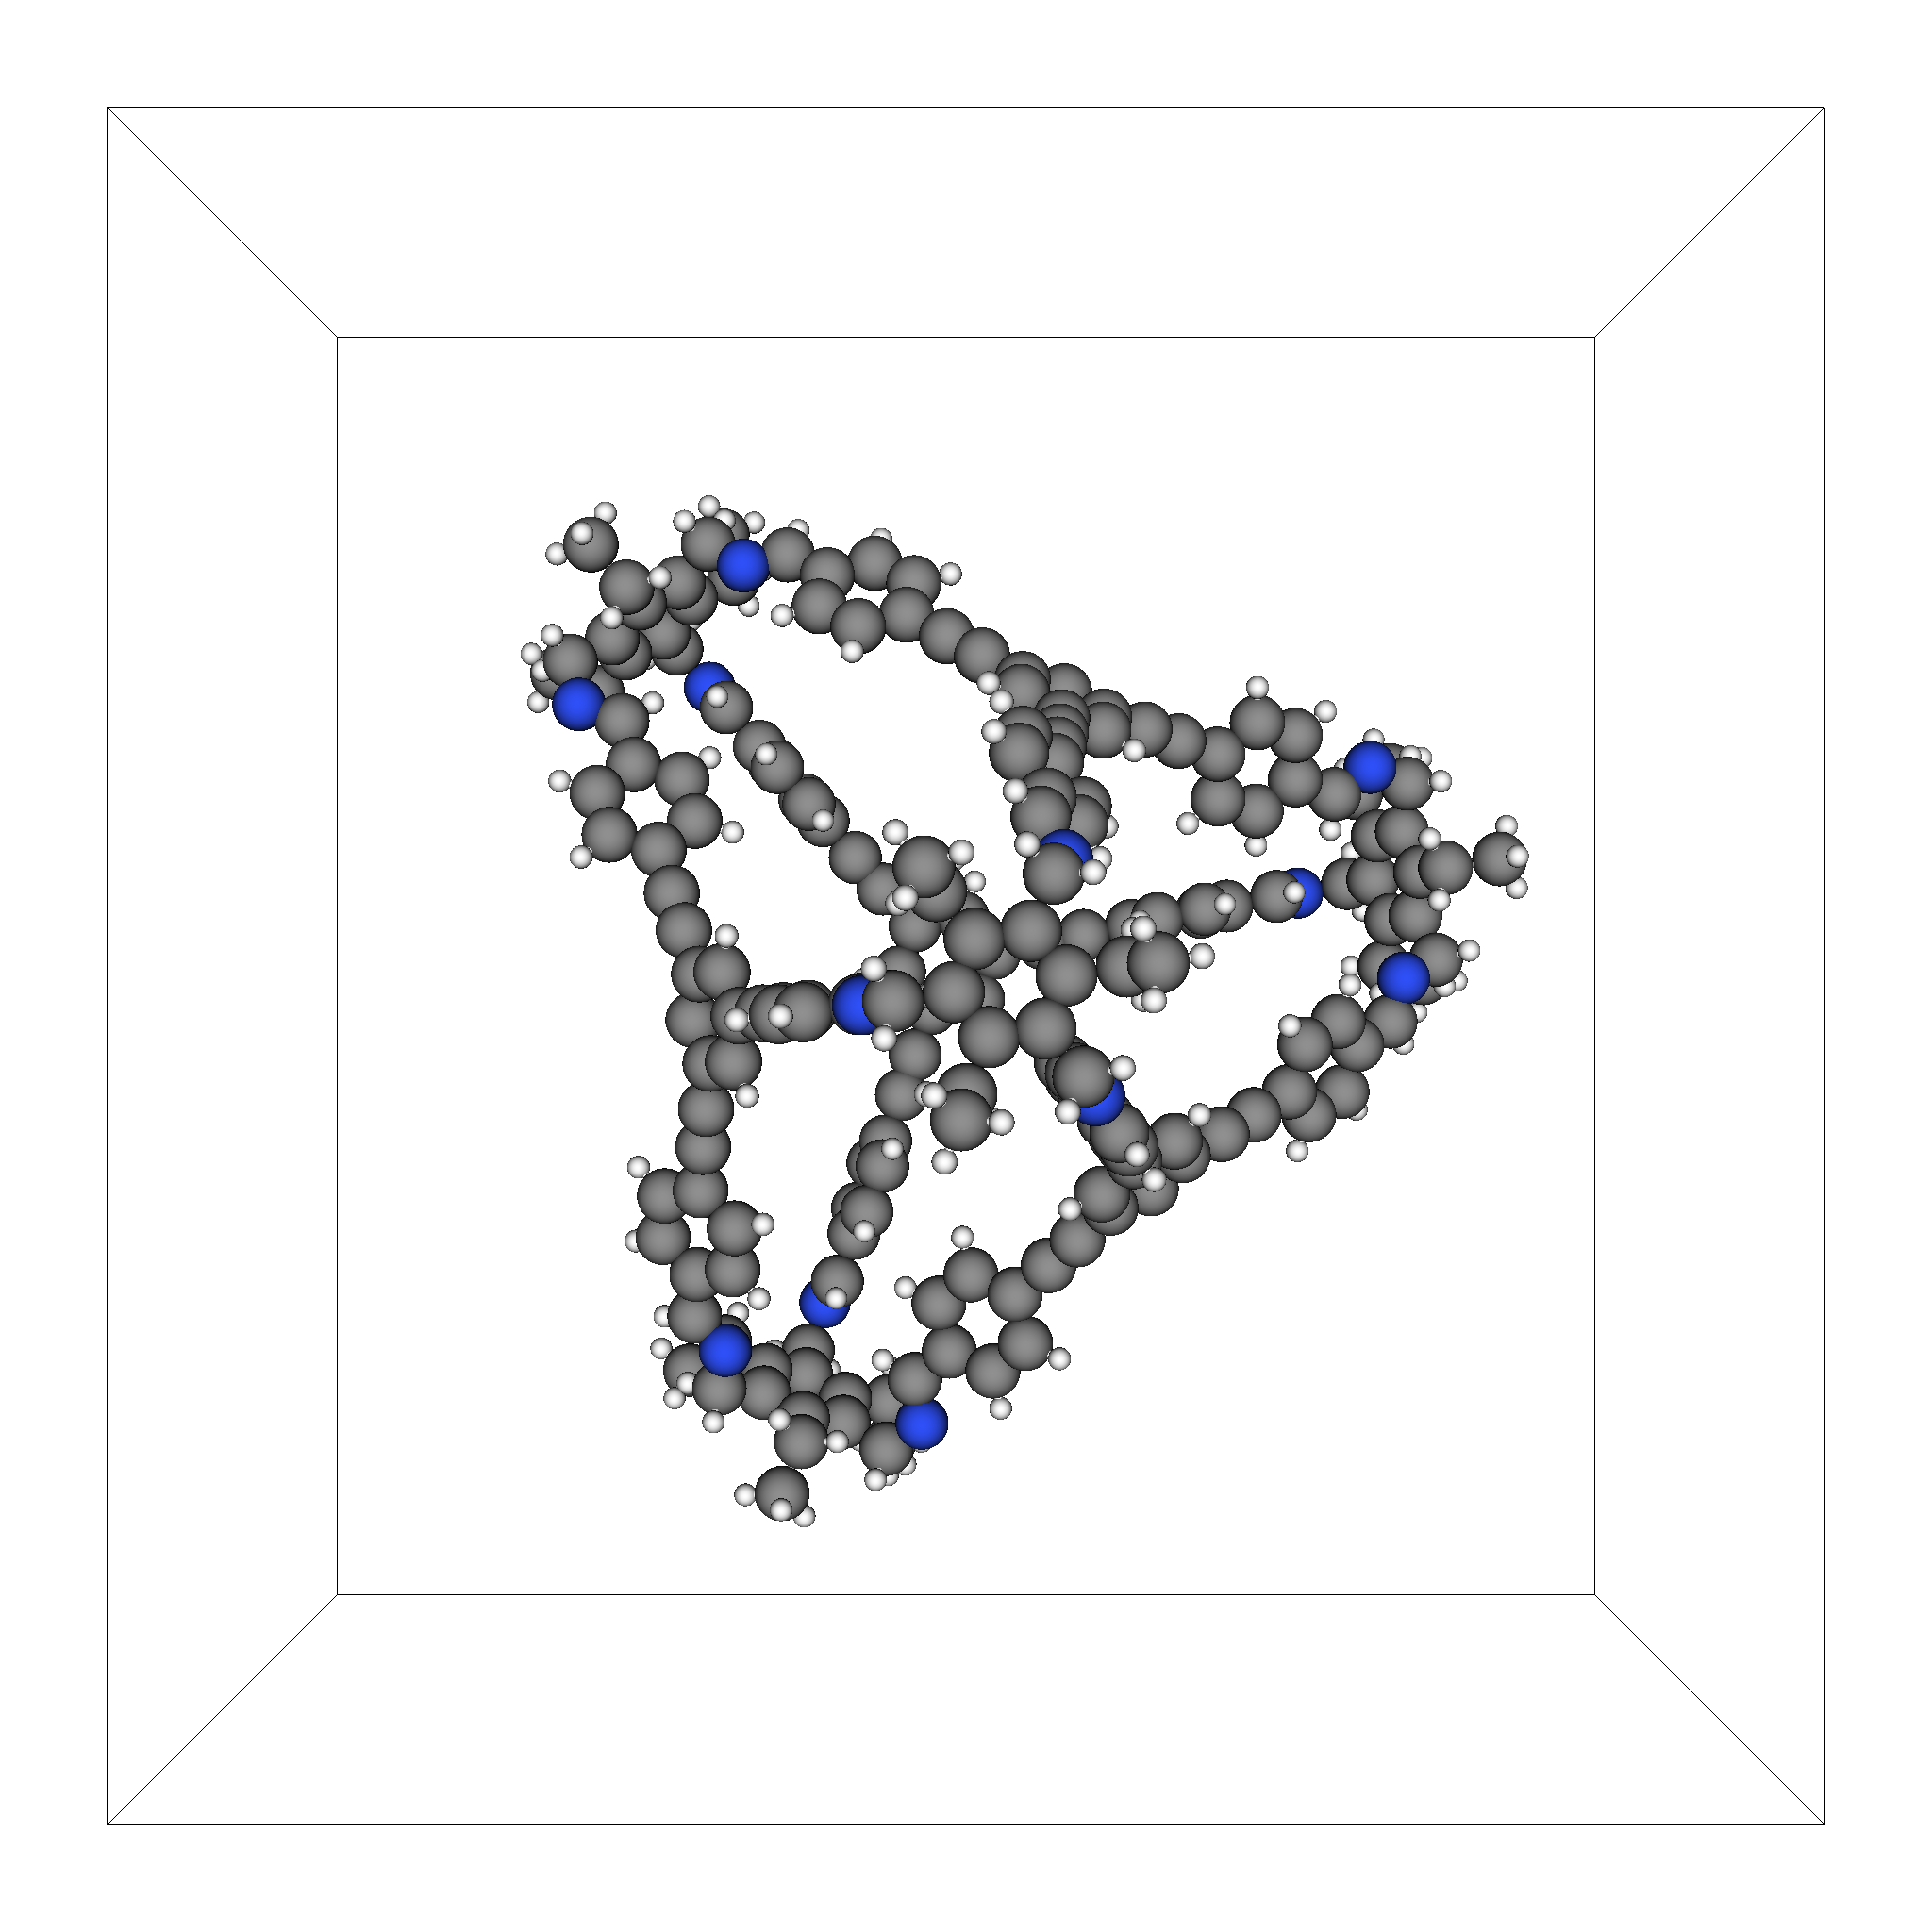
\includegraphics[width=0.25\columnwidth]{../final_aligned_cages/C25.png}}
\subfloat[C26]{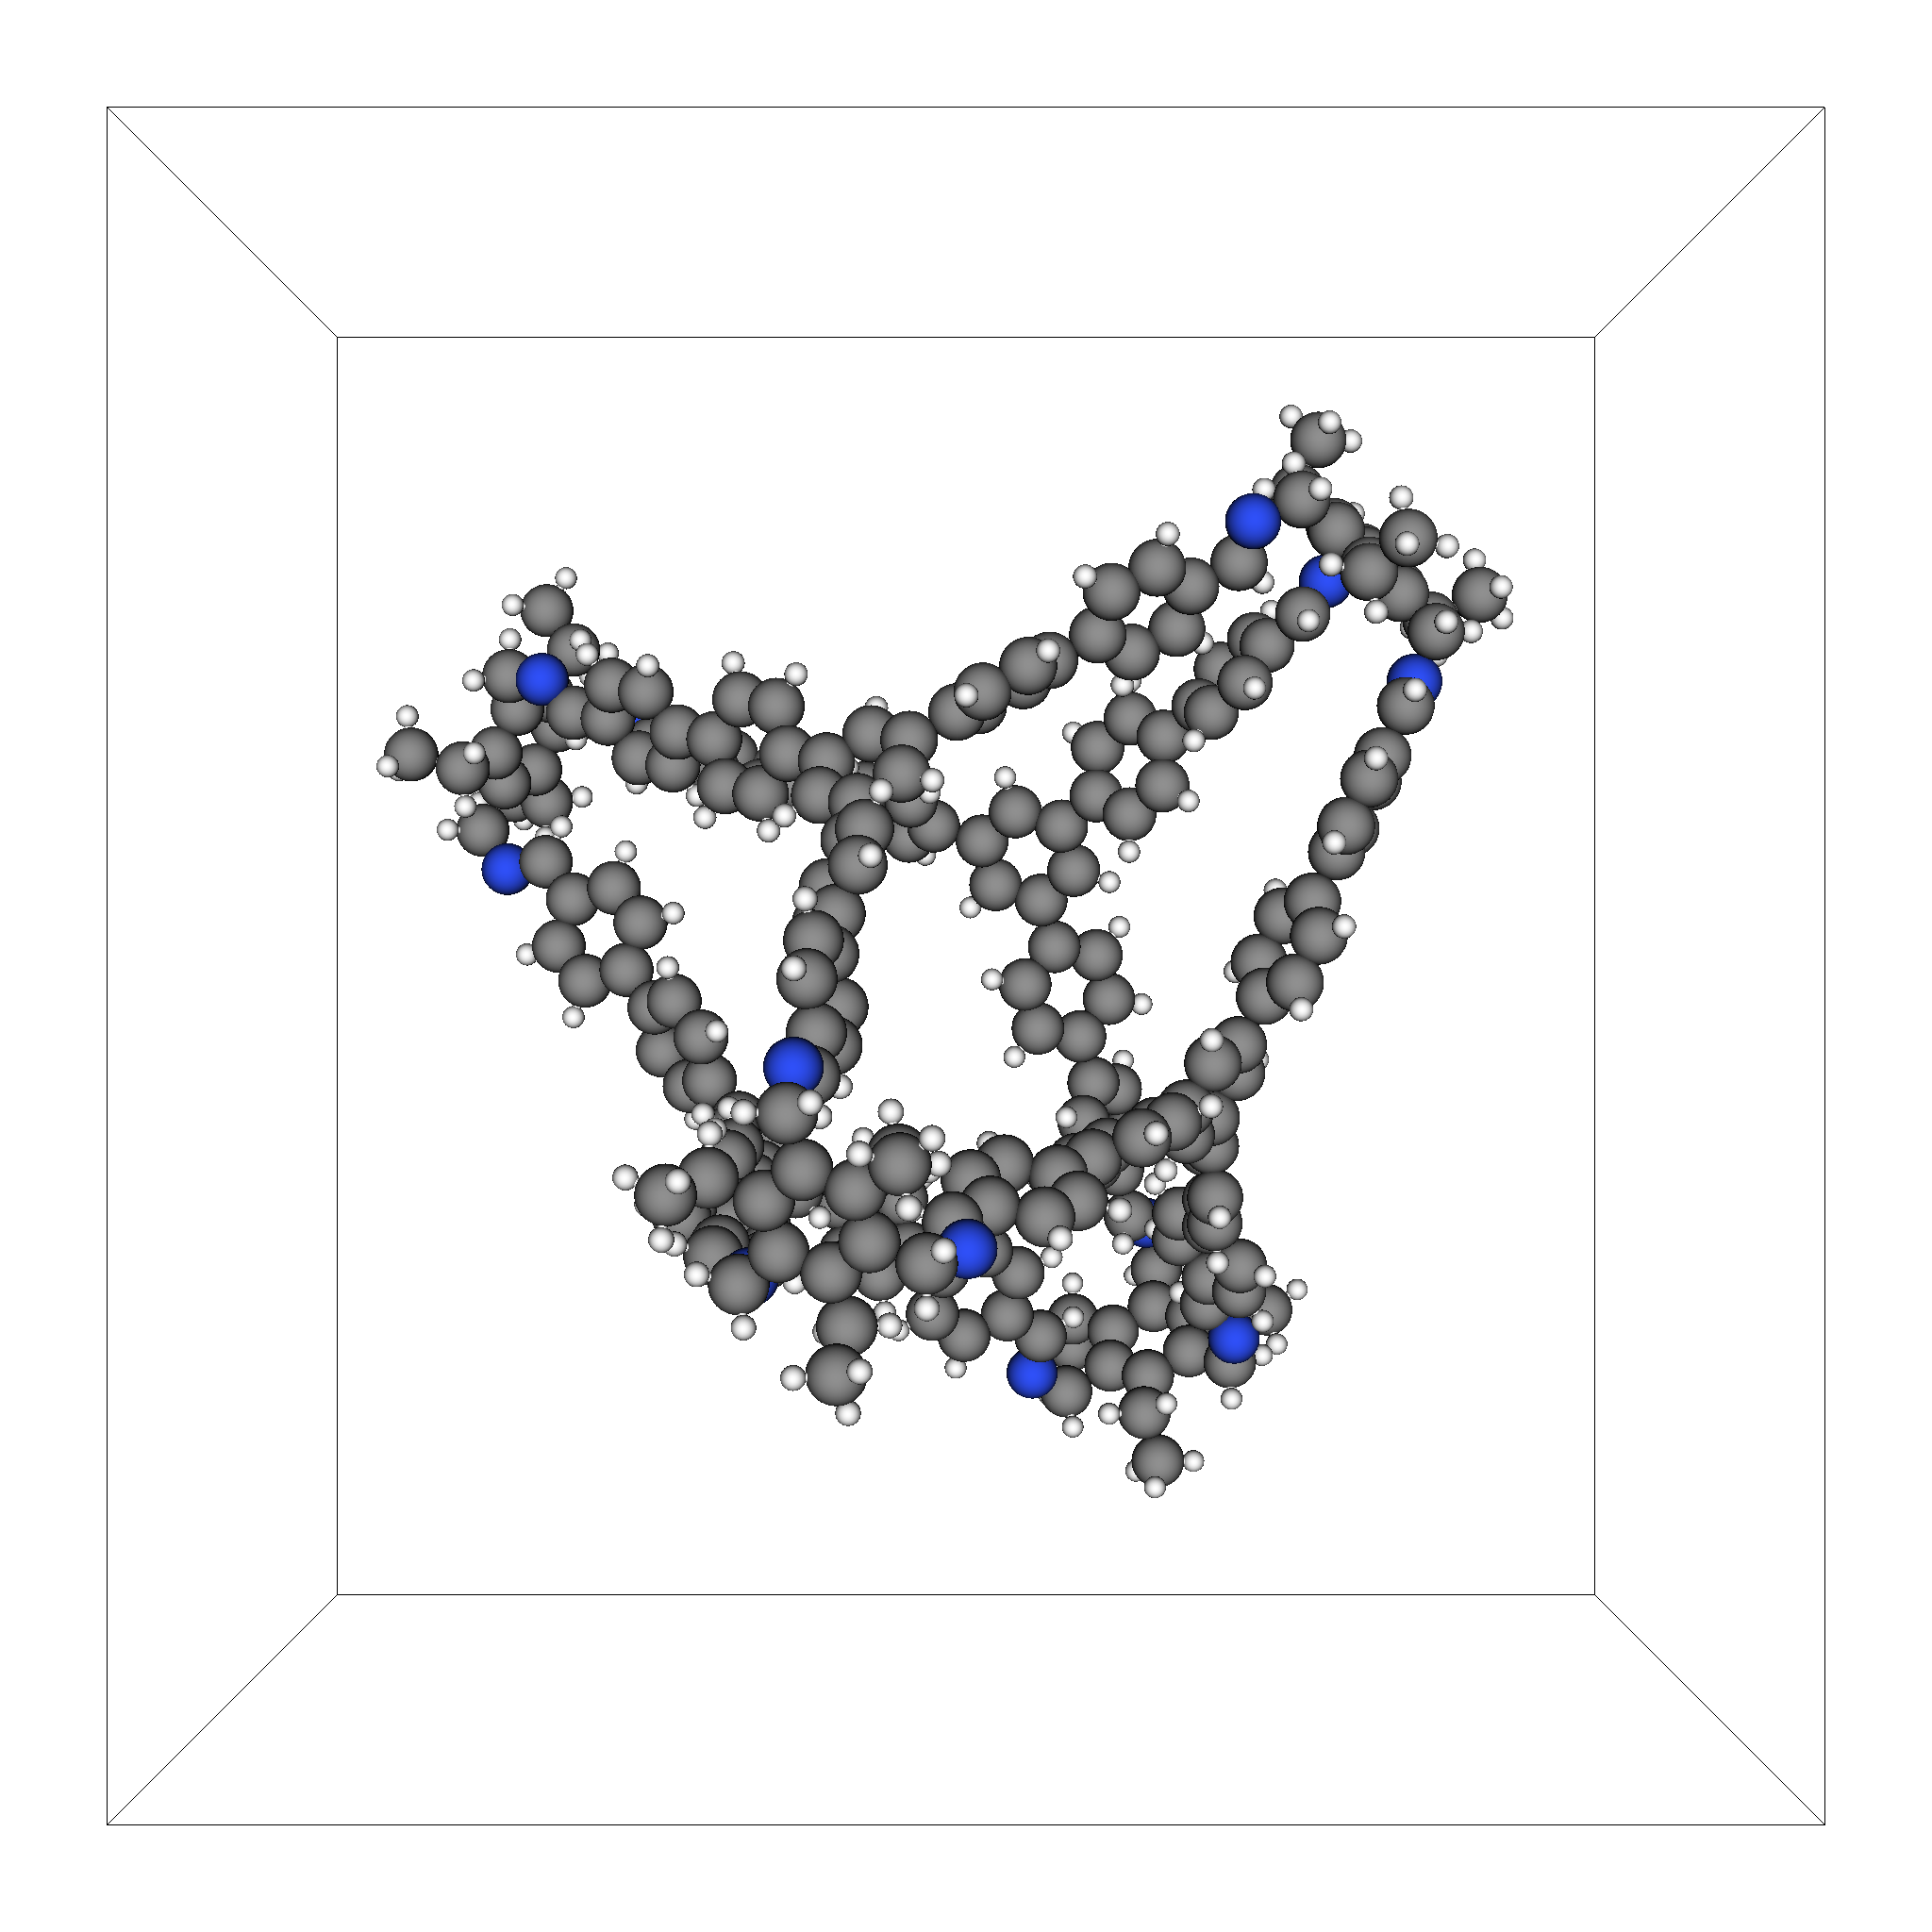
\includegraphics[width=0.25\columnwidth]{../final_aligned_cages/C26.png}}
\qquad
\subfloat[C2]{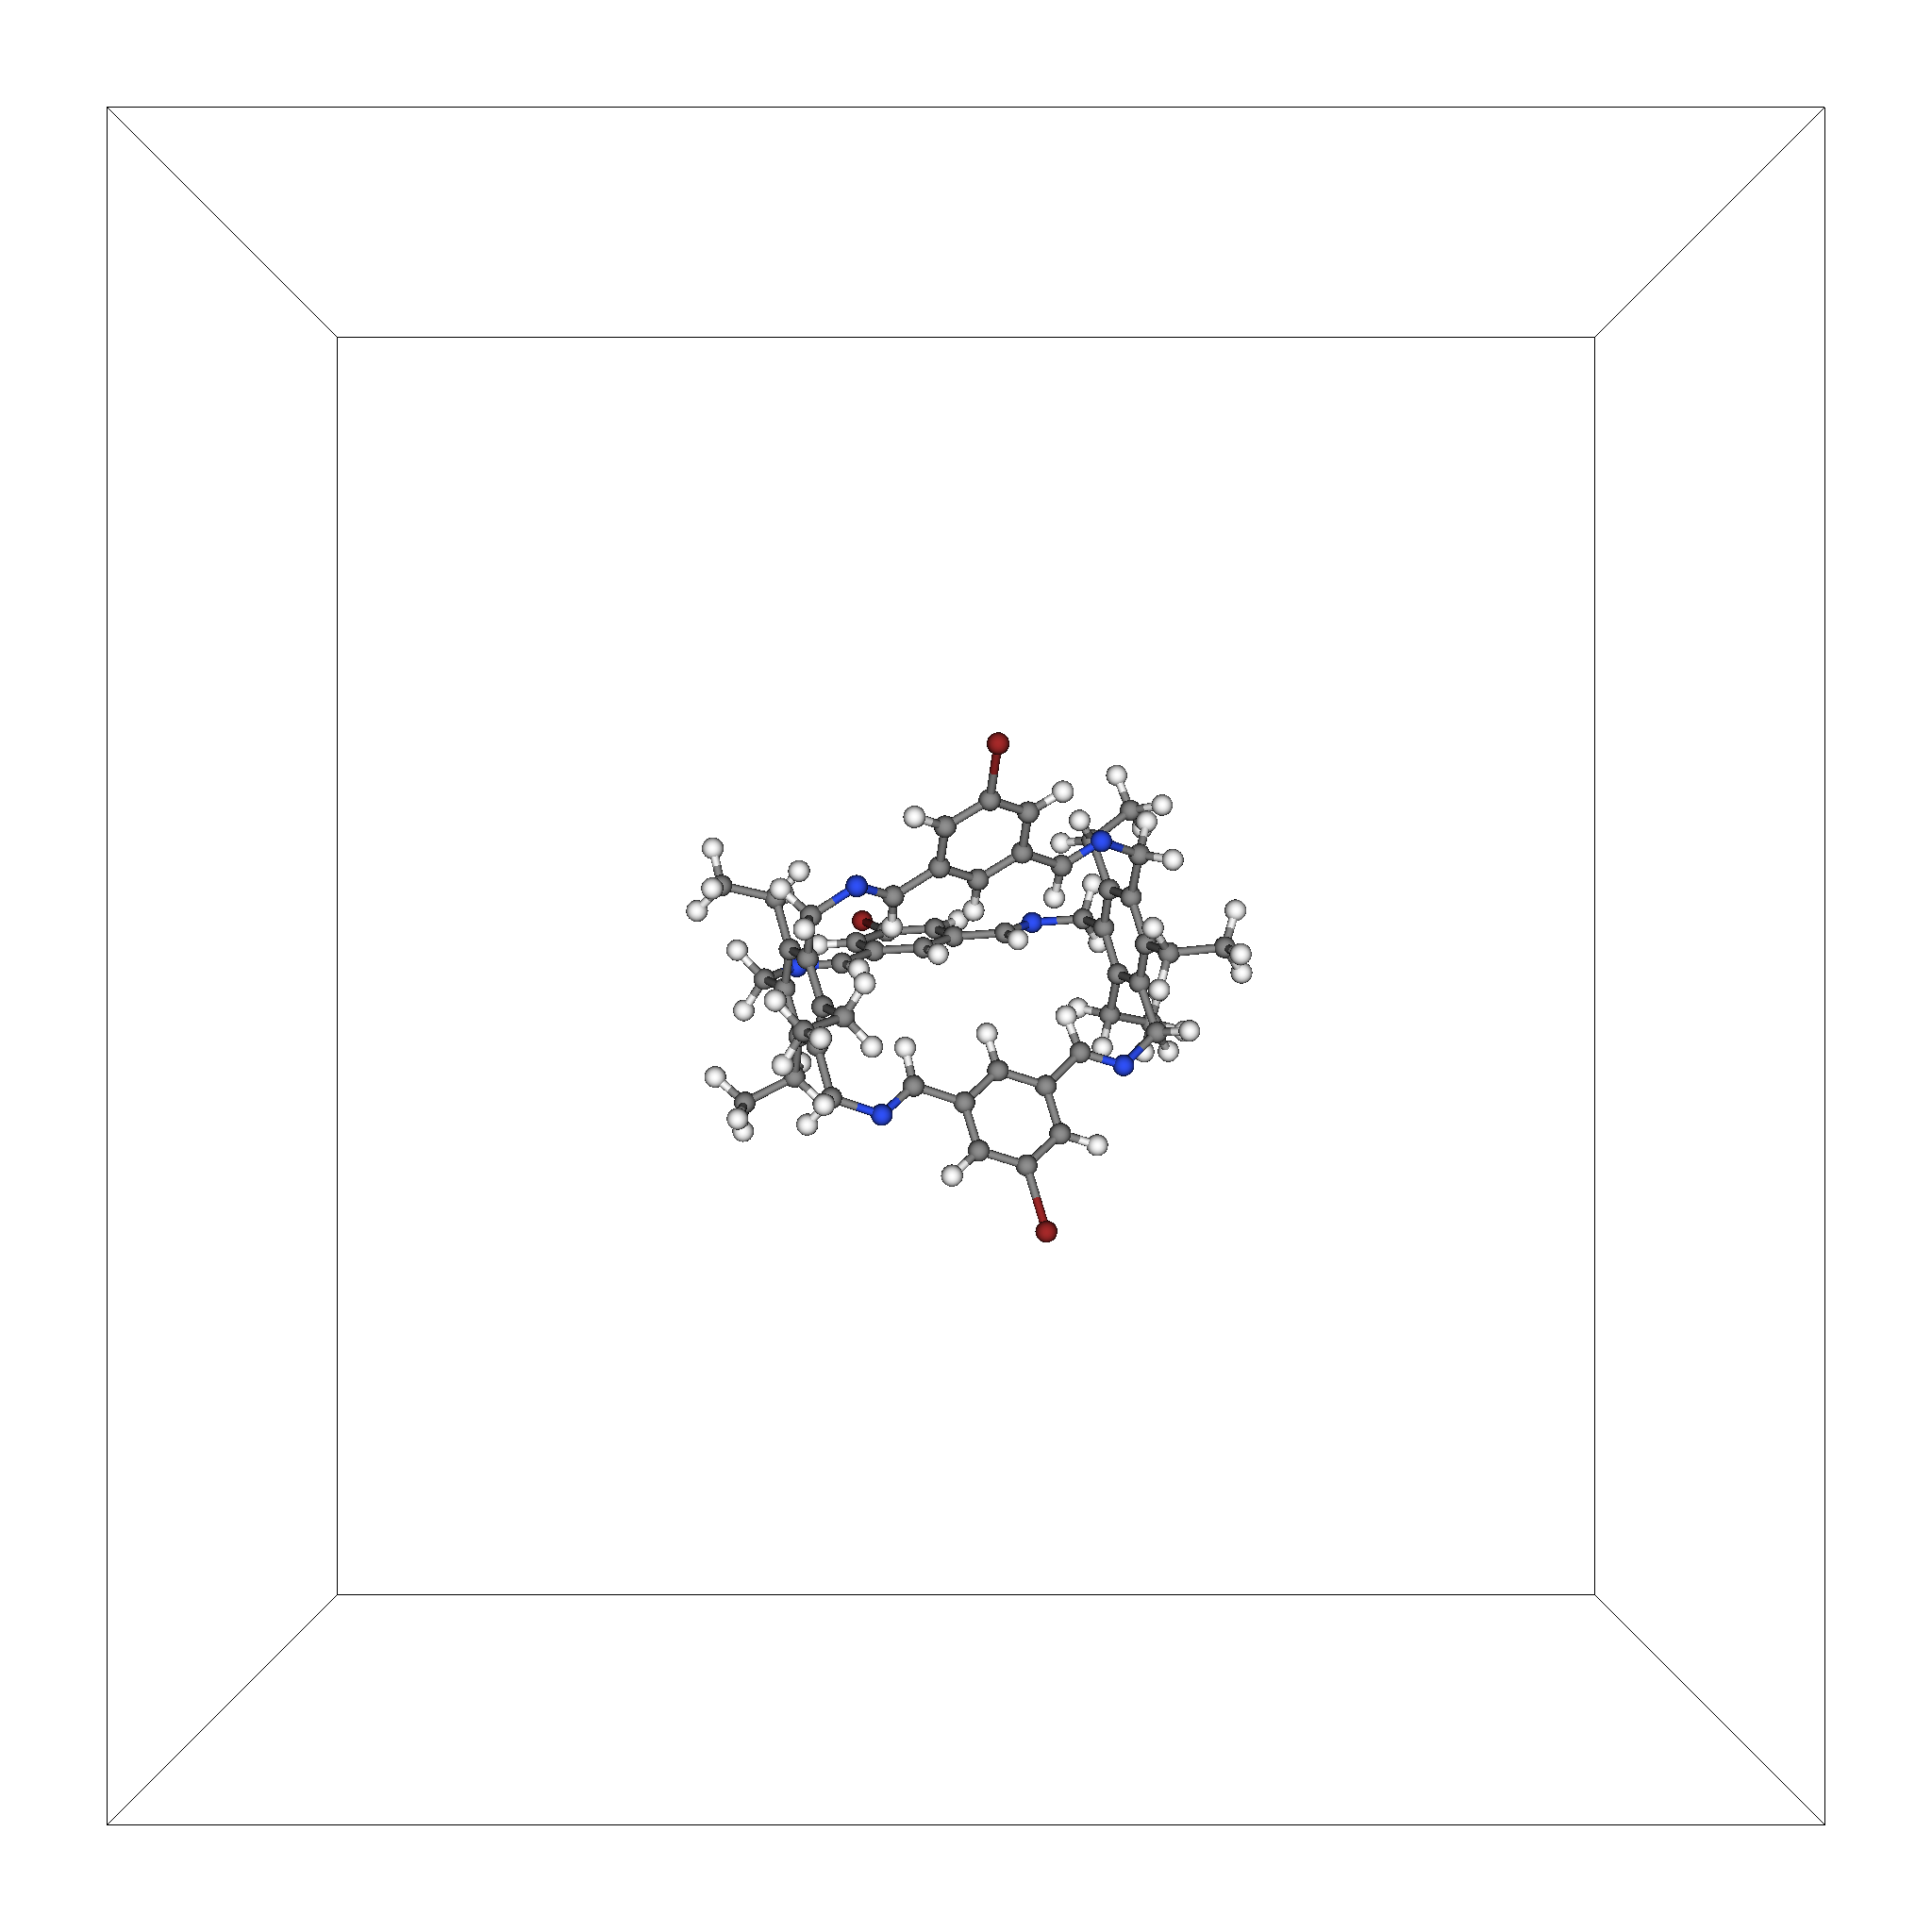
\includegraphics[width=0.25\columnwidth]{../final_aligned_cages/C2.png}}
\subfloat[C4]{\includegraphics[width=0.25\columnwidth]{../final_aligned_cages/C4.png}}
\subfloat[C5]{\includegraphics[width=0.25\columnwidth]{../final_aligned_cages/C5.png}}
\qquad
\subfloat[C6]{\includegraphics[width=0.25\columnwidth]{../final_aligned_cages/C6.png}}
\subfloat[C8]{\includegraphics[width=0.25\columnwidth]{../final_aligned_cages/C8.png}}
\subfloat[C9]{\includegraphics[width=0.25\columnwidth]{../final_aligned_cages/C9.png}}
\qquad
\subfloat[CB5]{\includegraphics[width=0.25\columnwidth]{../final_aligned_cages/CB5.png}}
\subfloat[CB6]{\includegraphics[width=0.25\columnwidth]{../final_aligned_cages/CB6.png}}
\subfloat[CB7]{\includegraphics[width=0.25\columnwidth]{../final_aligned_cages/CB7.png}}
\phantomcaption \end{figure}
\begin{figure}
\ContinuedFloat \centering
\subfloat[CC10]{\includegraphics[width=0.25\columnwidth]{../final_aligned_cages/CC10.png}}
\subfloat[CC1]{\includegraphics[width=0.25\columnwidth]{../final_aligned_cages/CC1.png}}
\subfloat[CC2]{\includegraphics[width=0.25\columnwidth]{../final_aligned_cages/CC2.png}}
\qquad
\subfloat[CC3]{\includegraphics[width=0.25\columnwidth]{../final_aligned_cages/CC3.png}}
\subfloat[CC4]{\includegraphics[width=0.25\columnwidth]{../final_aligned_cages/CC4.png}}
\subfloat[CC5]{\includegraphics[width=0.25\columnwidth]{../final_aligned_cages/CC5.png}}
\qquad
\subfloat[CC9]{\includegraphics[width=0.25\columnwidth]{../final_aligned_cages/CC9.png}}
\subfloat[CD1]{\includegraphics[width=0.25\columnwidth]{../final_aligned_cages/CD1.png}}
\subfloat[CD2]{\includegraphics[width=0.25\columnwidth]{../final_aligned_cages/CD2.png}}
\qquad
\subfloat[CD3]{\includegraphics[width=0.25\columnwidth]{../final_aligned_cages/CD3.png}}
\subfloat[CP1]{\includegraphics[width=0.25\columnwidth]{../final_aligned_cages/CP1.png}}
\subfloat[CP3]{\includegraphics[width=0.25\columnwidth]{../final_aligned_cages/CP3.png}}
\phantomcaption \end{figure}
\begin{figure}
\ContinuedFloat \centering
\subfloat[CP4]{\includegraphics[width=0.25\columnwidth]{../final_aligned_cages/CP4.png}}
\subfloat[CP5]{\includegraphics[width=0.25\columnwidth]{../final_aligned_cages/CP5.png}}
\subfloat[DC1]{\includegraphics[width=0.25\columnwidth]{../final_aligned_cages/DC1.png}}
\qquad
\subfloat[GC1]{\includegraphics[width=0.25\columnwidth]{../final_aligned_cages/GC1.png}}
\subfloat[HC1]{\includegraphics[width=0.25\columnwidth]{../final_aligned_cages/HC1.png}}
\subfloat[IC1]{\includegraphics[width=0.25\columnwidth]{../final_aligned_cages/IC1.png}}
\qquad
\subfloat[IC2]{\includegraphics[width=0.25\columnwidth]{../final_aligned_cages/IC2.png}}
\subfloat[MC1]{\includegraphics[width=0.25\columnwidth]{../final_aligned_cages/MC1.png}}
\subfloat[MC2]{\includegraphics[width=0.25\columnwidth]{../final_aligned_cages/MC2.png}}
\qquad
\subfloat[MC3]{\includegraphics[width=0.25\columnwidth]{../final_aligned_cages/MC3.png}}
\subfloat[MC4]{\includegraphics[width=0.25\columnwidth]{../final_aligned_cages/MC4.png}}
\subfloat[MC5]{\includegraphics[width=0.25\columnwidth]{../final_aligned_cages/MC5.png}}
\phantomcaption \end{figure}
\begin{figure}
\ContinuedFloat \centering
\subfloat[MC6]{\includegraphics[width=0.25\columnwidth]{../final_aligned_cages/MC6.png}}
\subfloat[MC7]{\includegraphics[width=0.25\columnwidth]{../final_aligned_cages/MC7.png}}
\subfloat[NC1]{\includegraphics[width=0.25\columnwidth]{../final_aligned_cages/NC1.png}}
\qquad
\subfloat[NC2]{\includegraphics[width=0.25\columnwidth]{../final_aligned_cages/NC2.png}}
\subfloat[RCC1a]{\includegraphics[width=0.25\columnwidth]{../final_aligned_cages/RCC1a.png}}
\subfloat[RCC1b]{\includegraphics[width=0.25\columnwidth]{../final_aligned_cages/RCC1b.png}}
\qquad
\subfloat[RCC1c]{\includegraphics[width=0.25\columnwidth]{../final_aligned_cages/RCC1c.png}}
\subfloat[RCC1d]{\includegraphics[width=0.25\columnwidth]{../final_aligned_cages/RCC1d.png}}
\subfloat[RCC3a]{\includegraphics[width=0.25\columnwidth]{../final_aligned_cages/RCC3a.png}}
\qquad
\subfloat[RCC3b]{\includegraphics[width=0.25\columnwidth]{../final_aligned_cages/RCC3b.png}}
\subfloat[WC1]{\includegraphics[width=0.25\columnwidth]{../final_aligned_cages/WC1.png}}
\subfloat[WC2]{\includegraphics[width=0.25\columnwidth]{../final_aligned_cages/WC2.png}}
\phantomcaption \end{figure}
\begin{figure}
\ContinuedFloat \centering
\subfloat[WC3]{\includegraphics[width=0.25\columnwidth]{../final_aligned_cages/WC3.png}}
\subfloat[WC4]{\includegraphics[width=0.25\columnwidth]{../final_aligned_cages/WC4.png}}
\caption{Visualizations of the structures of all 74 porous organic cage molecules analyzed in this study.
    The \texttt{.xyz} files of these cages are from Miklitz et al. and Greenaway et al. \cite{miklitz2017computational,greenaway2018high};
    see these references for the naming conventions. The cages are visualized in their centered and aligned states
    in the $[-20,20]^3$ $\angstrom$
    snapshot box in preparation for taking the 3D cage cavity image.}
\label{fig:allcagesdetailed}
\end{figure}


\newpage
\clearpage

\section{Safety statement}
As this research is all computational in nature, no unexpected or unusually high safety hazards were encountered.

\clearpage

\bibliography{bibfile}
\end{document}
